\documentclass{SIAMbook2023}

% ============================================================================
% Learning with AI: A Framework for Students, Instructors, and Universities
%   From Graduate Mathematics to STEM Education, Departmental Practice, and Institutional Policy
% Single bound volume (Parts I, II, III) - SIAM Publishing Submission
% Author: James M. Hyman, Tulane University
% v4_30_17 - August 2026 (current. McKinley acknowledgment: promoted from the grouped closing sentence to the detailed tier, two findings, wording ruled by Mac; the grouped closer now reads Joshua Agbomola alone. Prior: v4_30_16 wrapper-coupling fold.)
% ============================================================================

% Draft/production toggle: set \preliminaryversionfalse for the submission build.
\newif\ifpreliminaryversion
\preliminaryversiontrue

% Fonts and encoding
\usepackage[T1]{fontenc}
\usepackage[utf8]{inputenc}
\usepackage{times}
\renewcommand{\sfdefault}{phv}

% Core packages
\usepackage{amsmath,amssymb}
\usepackage{graphicx}
\usepackage{float}
\usepackage{array}
\usepackage{booktabs}
\usepackage{longtable}
\usepackage{tabularx}
\usepackage{enumitem}
\usepackage{xcolor}
\usepackage{microtype}

% Bibliography (single shared bibliography for the bound volume)
\usepackage[numbers,sort&compress]{natbib}

% TikZ for figures
\usepackage{tikz}
\usetikzlibrary{positioning,arrows.meta,shapes.geometric,calc,fit,backgrounds,decorations.pathreplacing,decorations.markings,patterns}

% Hyperlinks and cross-references
\usepackage[hidelinks]{hyperref}
\emergencystretch=10em
\def\UrlBreaks{\do\/\do\-\do\_\do\.\do\=\do\&\do\?\do\#\do\:}
\usepackage[nameinlink,noabbrev]{cleveref}

% Page layout
\setlist[itemize]{leftmargin=1.5em,itemsep=0.25em,topsep=0.25em}
\setlist[enumerate]{leftmargin=1.7em,itemsep=0.25em,topsep=0.25em}
\setlist[description]{leftmargin=1.8em,labelsep=0.6em,itemsep=0.35em,topsep=0.35em}
\renewcommand{\arraystretch}{1.25}

% Header and footer
% running heads handled by SIAMbook2023 class

% Visual conventions
\definecolor{guideblue}{RGB}{25,70,120}
\definecolor{lightgray}{RGB}{245,245,245}
\definecolor{darkgray}{RGB}{70,70,70}

% Assignment-category colors: traffic-light palette plus blue
% for the orthogonal AIS category. Print-safe contrast tested; adjust hue values
% here to update all NAI/AIT/AIC/AIS occurrences globally.
\definecolor{catNAI}{RGB}{180,30,30}    % NAI - red (no AI)
\definecolor{catAIT}{RGB}{140,105,0}    % AIT - dark amber; 5.08:1 on white, clears WCAG AA normal text (was 180,135,0 at 3.28:1)
\definecolor{catAIC}{RGB}{30,130,60}    % AIC - green (full collaboration)
\definecolor{catAIS}{RGB}{25,70,120}    % AIS - blue (off-spectrum: AI as study)

% Hyperref metadata
\hypersetup{
  pdftitle={Learning with AI: A Framework for Students, Instructors, and Universities},
  pdfauthor={James M. Hyman},
  pdfsubject={AI-assisted learning at colleges and universities},
  pdfkeywords={AI-assisted learning, AI literacy, higher education, STEM education, quantitative sciences, computational sciences, assessment, academic integrity, graduate mathematics, CAT framework, Student's Trilemma, Learning Spiral}
}

% Custom commands
% Index machinery. \keyterm now also emits a bolded index entry at its defining site.
% Optional argument supplies a custom index key: \keyterm[polished hollow!instructor]{instructor polished hollow}
\usepackage{imakeidx}
\makeindex[intoc=true, title=Index, columns=2]
\makeatletter
\newcommand{\keyterm}[2][\relax]{%
  \textbf{#2}%
  \ifx\relax#1\index{#2|textbf}\else\index{#1|textbf}\fi}
\makeatother
\newcommand{\studentprompt}[1]{\begin{quote}\small\itshape #1\end{quote}}
\newcommand{\instructorprompt}[1]{\begin{quote}\small\itshape #1\end{quote}} % intentionally mirrors \studentprompt; kept distinct for semantic tagging
\newcommand{\courselabel}[1]{\textbf{#1}}
\newcommand{\checkitem}{\item[$\square$]}

% Colored-acronym macros for assignment categories
% Each macro renders the acronym in its category color, bold for emphasis.
% Single source of truth: edit color above to propagate everywhere.
\newcommand{\NAI}{\textcolor{catNAI}{\textbf{NAI}}}
\newcommand{\AIT}{\textcolor{catAIT}{\textbf{AIT}}}
\newcommand{\AIC}{\textcolor{catAIC}{\textbf{AIC}}}
\newcommand{\AIS}{\textcolor{catAIS}{\textbf{AIS}}}

% Shared TikZ figure styles
% Two-color palette: guideblue for emphasis, darkgray for secondary; lightgray for fills.
\tikzset{
  framework-node/.style={draw=guideblue, thick, rounded corners=2pt,
    minimum width=2.6cm, minimum height=0.95cm, font=\small, align=center,
    inner sep=4pt},
  emphasis-node/.style={draw=guideblue, very thick, fill=lightgray,
    rounded corners=2pt, minimum width=2.6cm, minimum height=0.95cm,
    font=\small, align=center, inner sep=4pt},
  secondary-node/.style={draw=darkgray, thick, rounded corners=2pt,
    minimum width=2.4cm, minimum height=0.85cm, font=\footnotesize, align=center,
    inner sep=3pt},
  flow-arrow/.style={-{Stealth[length=2.4mm]}, thick, draw=darkgray},
  emphasis-arrow/.style={-{Stealth[length=2.6mm]}, very thick, draw=guideblue},
  seed-node/.style={draw=guideblue, line width=1.1pt, fill=guideblue!12, rounded corners=3pt,
    minimum width=2.3cm, minimum height=0.95cm, font=\small\bfseries, align=center, inner sep=3pt, text=guideblue},
  bidir-arrow/.style={{Stealth[length=2mm]}-{Stealth[length=2mm]}, thick, draw=darkgray},
  caption-text/.style={font=\small\itshape, color=darkgray},
  region-box/.style={draw=darkgray, dashed, rounded corners=3pt, inner sep=8pt},
  axis-label/.style={font=\small, align=center, color=darkgray},
  quadrant-label/.style={font=\footnotesize\itshape, align=center, color=darkgray, text width=3.4cm}
}

% Dialogue environment for annotated student-AI exchanges
\newenvironment{dialogue}[1]%
  {\par\medskip\noindent\textbf{\textcolor{guideblue}{#1}}\par\smallskip
   \begin{list}{}{\setlength{\leftmargin}{1.5em}\setlength{\rightmargin}{0.5em}\setlength{\itemsep}{0.4em}\setlength{\topsep}{0pt}}}
  {\end{list}\par\medskip}
\newcommand{\studentturn}[1]{\item[\textbf{Student.}] #1}
\newcommand{\aiturn}[1]{\item[\textbf{AI.}] \textit{#1}}
\newcommand{\dialogueannotate}[1]{\par\smallskip\hspace{2em}\textcolor{darkgray}{\footnotesize\textsf{$\rightarrow$ #1}}\par}

% Epigraph macro: centered italic block placed below major openings (the Foreword, the
% three Parts, and the four Appendices) and at selected section openings. The epigraphs are
% original maxims, except the line in the Dangerous-uses section, which is attributed in place.
\newcommand{\bookepigraph}[1]{%
  \begin{center}%
    \begin{minipage}{0.78\textwidth}%
      \centering\itshape #1%
    \end{minipage}%
  \end{center}%
  \vspace{0.6em}%
}

\title{\textbf{Learning with AI}\\[0.4em]
\large A Framework for Students, Instructors, and Universities\\[0.25em]
\normalsize\textit{From Graduate Mathematics to STEM Education, Departmental Practice, and Institutional Policy}}
\author{James M. Hyman \\
\small Tulane University \\
\small New Orleans, Louisiana}
\date{\ifpreliminaryversion\today\\\small\textit{Preliminary version; for review only}\fi}

\begin{document}
% Index cross-references (see-entries; page numbers are discarded by makeindex,
% so position is free, but they must ship out before \printindex closes the .idx).
\index{cheating|see{academic integrity}}\index{faculty buy-in|see{buy-in, faculty}}\index{part-time faculty|see{adjunct faculty}}\index{compensation|see{stipends}}\index{RCM|see{Responsibility Center Management}}\index{retrieval practice|see{practice testing}}\index{detectors|see{AI detectors}}\index{trilemma|see{Trilemma}}\index{AI as Object of Study|see{assignment categories}}\index{compact, student|see{Student Compact}}\index{scope, course|see{course scope}}

\begin{titlepage}
\thispagestyle{empty}
\setcounter{page}{0}
\vspace*{2.5cm}
\begin{center}
{\Huge\bfseries Learning with AI}\\[1.2em]
{\Large A Framework for Students, Instructors, and Universities}\\[0.6em]
{\large\itshape From Graduate Mathematics to STEM Education,\\Departmental Practice, and Institutional Policy}

\vfill

{\Large James M. Hyman}\\[0.4em]
{\normalsize Tulane University}\\
{\normalsize New Orleans, Louisiana}

\vspace{2.5cm}

% OVERFULL-BENIGN (S-alpha 2026-07-13): the ~519pt overfull logged for this block is a glue
% artifact of the centered construction; the page renders clean. Do not chase.
\ifpreliminaryversion
{\small \today}\\[0.4em]
{\small\itshape Preliminary version; for review only}
\fi
\end{center}
\end{titlepage}

\frontmatter

% ============================================================================
% UNIFIED ABSTRACT
% ============================================================================

\section*{About this book}
\addcontentsline{toc}{section}{About this book}
This book presents a framework for AI-assisted learning at colleges and universities. It is written for three audiences: students learning to use AI without surrendering their own thinking, instructors designing courses that remain intellectually honest under AI access, and academic departments and institutions developing coherent policy and practice. The framework was developed for graduate mathematics, and its primary audience is the quantitative and computational sciences. Its principles extend to undergraduate STEM education and to departmental and institutional governance, and the examples are especially detailed for STEM and research-intensive courses. Much of the guidance transfers to writing, the humanities, the social sciences, professional programs, and creative work as well, though the book does not set out to be a manual for those fields.

The framework rests on three commitments. First, courses must distinguish what students can do independently from what they can do with AI assistance, and assess each in proportion to the goals of the course. Second, AI use should be visible, verified, and disclosed rather than hidden or assumed. Third, students, instructors, and institutions need shared vocabulary if AI policy is to function in practice.

The book is organized in three Parts. Part I, the Student Guide, gives undergraduate and graduate students a practical compact for using AI as tutor, critic, and study partner without giving up the thinking each course is meant to build. Part II, the Instructor Guide, gives faculty assignment-design tools, assessment models for small and large classes, and rubrics for AI-aware grading. Part III, the Departmental and Institutional Guide, gives departments and universities shared policy language, privacy safeguards, equity considerations, and adoption workflows that work at the level where most decisions are actually made. Three Parts share a single vocabulary: Core Competence, AI-assisted Practice, and Trustworthiness; the Learning Spiral; and the assignment categories No AI (NAI), AI as Tutor (AIT), AI as Collaborator (AIC), and AI as Object of Study (AIS). This book was itself prepared with AI assistance, disclosed in full in Appendix~\ref{app:disclosure}.

% ============================================================================
% AI ASSISTANCE DISCLOSURE (single, master version for the bound volume)
% ============================================================================

\section*{How to read this book}
\addcontentsline{toc}{section}{How to read this book}

This book is one bound volume in three Parts. Each Part is written for a different reader, and each Part can be read on its own.

Three short descriptions follow, one for each reader. Find the one that sounds like your week.

\textbf{You got the right answer and could not explain it.} An AI produced something clean, and the next day you could not reconstruct it. Page~\pageref{subsec:config-before-after} shows a student asking for the limit of $(\sin x)/x$ and getting the whole proof back at once. The same page shows the same model, asked the same question, answering with a question instead. Nothing about the AI changed. What changed was what it had been told. Part~\ref{part:student} begins on page~\pageref{part:student}.

\textbf{You cannot tell what the student did.} The work is polished and the grade is a guess. Page~\pageref{i:subsec:seeded-error-check} describes planting a fixed number of errors in an AI-written passage and asking students to find them. The score is the detection rate. A student who finds four of five has shown you something a clean submission never shows. Part~\ref{part:instructor} collects instruments like that one, and it begins on page~\pageref{part:instructor}.

\textbf{You have to write a policy and the evidence is thin.} Claims about AI in education arrive faster than the studies behind them. Page~\pageref{u:tab:evidence-status} takes this book's own claims one at a time and marks each one established, inferred, or untested. Part~\ref{part:institutional} builds departmental practice on the first two Parts and says where it is guessing. It begins on page~\pageref{part:institutional}.

Most students meet Part~\ref{part:student} because an instructor assigned it. That is how the book is designed to travel, and each chapter can be assigned on its own when a course reaches its topic. A student who found this book alone can read it the same way.

Each description above points you to your own Part. The book also asks you to look at the other two, and that request is not incidental; it is the reason this is one book (\cref{fig:three-scales}). Policy, teaching, and learning are all being worked out at the same time, and no group yet holds settled expertise to hand to the others. The reading just described runs in the familiar direction, with those who teach and those who set policy reading to understand the work their decisions shape. It is meant to run the other way as well. A student who reads the instructor Part is better placed to tell a teacher what is working, at a time when many instructors are still finding their footing with these tools. An instructor who reads the institutional Part is better placed to tell a chair or dean what classroom policy should say. The transformation these Parts describe is a collective one, and it will go better if each group can see it through the others' eyes. One thread runs through all three. Each group acts on what it is scored on: a student on the grade, an instructor on what the department counts, a department on how the budget rewards enrollment. That is how the coupling works, and it is why a fix at one scale can be undone at another.

\begin{figure}[H]
\centering
\resizebox{\textwidth}{!}{%
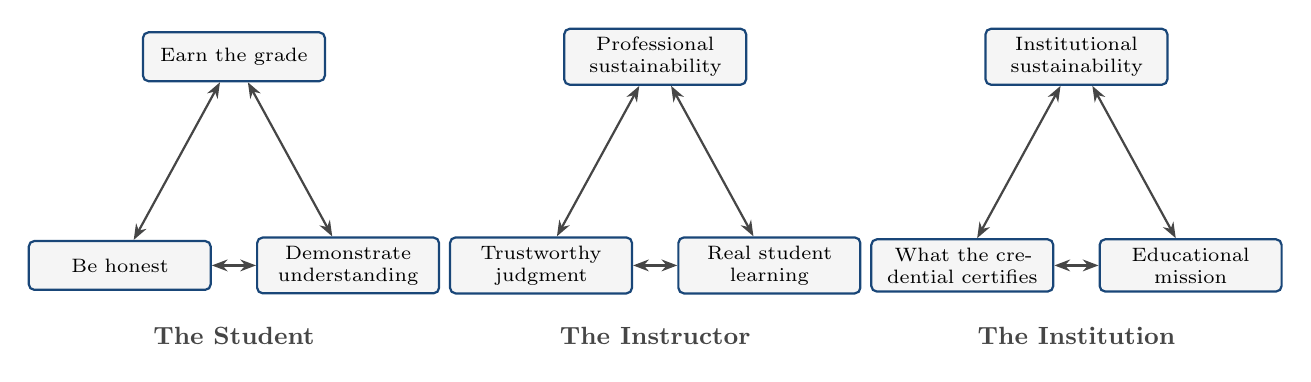
\begin{tikzpicture}[ov/.style={draw=guideblue, thick, fill=lightgray, rounded corners=2pt, font=\scriptsize, align=center, inner sep=3pt, text width=2.1cm, minimum height=0.62cm}]
\foreach \cx/\aud/\tg/\bl/\br/\i in {%
  -5.35/The Student/Earn the grade/Be honest/Demonstrate understanding/A,%
  0/The Instructor/Professional sustainability/Trustworthy judgment/Real student learning/B,%
  5.35/The Institution/Institutional sustainability/What the credential certifies/Educational mission/C%
}{
  \node[ov] (t\i) at (\cx,1.6) {\tg};
  \node[ov] (l\i) at (\cx-1.45,-1.05) {\bl};
  \node[ov] (r\i) at (\cx+1.45,-1.05) {\br};
  \draw[bidir-arrow] (t\i) -- (l\i);
  \draw[bidir-arrow] (t\i) -- (r\i);
  \draw[bidir-arrow] (l\i) -- (r\i);
  \node[font=\small\bfseries, color=darkgray] at (\cx,-1.95) {\aud};
}
\end{tikzpicture}
}
\caption{\textbf{One structure, three scales.} Each group's three goals are named at the corners, in the same orientation so the corners line up: a viability goal at the top, an honesty goal at the lower left, and a genuine-learning goal at the lower right. The three edges carry the same failure modes at every scale (polished hollow, strategic compliance, honest risk). Policy, teaching, and learning are coupled: what each group does shapes, and is shaped by, the others.}
\label{fig:three-scales}
\end{figure}

All three Parts use the same vocabulary. The Preface introduces this vocabulary briefly. The full development of each term appears in the Part where the reader most needs it: Core Competence, AI-assisted Practice, and Trustworthiness in Part I; assignment categories and assessment models in Part II; institutional policy and adoption practice in Part III.

A reader looking for a single chapter to scan should consider the CAT framework section in Part I, the four assignment categories in Part II, or the CAT section in Part III, depending on role.

Readers who want a brief account of the learning-science principles this book operationalizes, including the calibration problem that AI use sharpens, should also see \cref{sec:learning-science} (How learning happens, and how AI changes it) early in Part~\ref{part:student}.

% ============================================================================
% ABOUT THE COMPANION REPOSITORY
% ============================================================================

Four appendices follow the three Parts. They are written for different readers, and none is required for the framework itself. Appendix~\ref{app:gmip} gives the graduate profile the book's categories were generalized from, for departments that want the source. Appendix~\ref{app:mae} turns that profile into an assessment framework for graduate mathematics. Appendix~\ref{app:sciwriting} covers AI-assisted scientific writing and is the one most graduate students and postdocs will want. Appendix~\ref{app:math-qr} is a quick reference for mathematics courses.

\section*{About the companion repository}
\addcontentsline{toc}{section}{About the companion repository}

This book has a companion repository at \texttt{github.com/machyman/hyman2026learning}, with a rendered site at \texttt{machyman.github.io/hyman2026learning}. The materials are permanently archived at \texttt{doi.org/10.5281/zenodo.21315920}. That address will keep working even if the repository moves. The repository hosts free, open-source materials that work alongside the book. Two are primary tools that students paste into AI applications. The Study Partner Protocol (SPP) is a prompt that turns the assistant into a study partner, one that helps the student learn rather than handing over finished work. Define Personal Preferences (DPP) is a walkthrough that helps a student configure their AI tool's persistent settings the first time they use it. The repository also gives instructors sample syllabus paragraphs, AI disclosure policies, and an adoption quickstart. Students receive standalone artifacts: a guide to sharing AI conversations with a teacher, disclosure templates, and the pre-submission checklist that appears in Part~\ref{part:student}.

The repository is organized in four folders, and \cref{tab:repo-map} shows what each one holds.

\begin{table}[H]
\centering
\caption{\textbf{What the companion repository holds.} Every folder is reachable from the repository's front page. Start in the folder that matches who you are, not the Part you are reading.}
\label{tab:repo-map}
\begin{tabularx}{\textwidth}{>{\raggedright\arraybackslash}X >{\raggedright\arraybackslash}X >{\raggedright\arraybackslash}X}
\toprule
\textbf{Folder} & \textbf{What it holds} & \textbf{For} \\
\midrule
\texttt{students/} & Two onboarding guides, the pre-submission checklist, disclosure templates, a guide to sharing AI conversations with a teacher, and worked study sessions in statistics, programming, physics, and mathematics & Students, and instructors choosing what to assign \\
\addlinespace
\texttt{instructors/} & A first-time teaching guide, a one-page assignment schedule, assignment templates, rubrics, assessment models, a semester redesign, and a faculty FAQ & Faculty, teaching assistants, course coordinators \\
\addlinespace
\texttt{institutions/} & A departmental adoption kit, a policy self-audit, and the regulatory landscape & Chairs, committees, teaching centers, administrators \\
\addlinespace
\texttt{companion/} & The Study Partner Protocol, Define Personal Preferences, and the other artifacts students paste into an AI tool & Students, assigned by instructors \\
\bottomrule
\end{tabularx}
\end{table}

The book and the repository are intended to be used together. The book teaches the framework; the repository hosts the operational artifacts. References from the book to specific companion materials appear throughout, in the form \texttt{companion/spp/}, \texttt{students/checklist.md}, and similar paths. The book remains under SIAM copyright; the materials in the repository are released under the MIT license and can be freely used, modified, adapted, translated, and redistributed with attribution. The repository will continue to evolve after publication; corrections to the book itself, if any are needed, appear in the repository's \texttt{ERRATA.md} file. The same file records post-publication status notes for time-sensitive references, so the bibliography's dated snapshot entries can age visibly rather than silently.

% ============================================================================
% ACKNOWLEDGMENTS
% ============================================================================

\section*{Acknowledgments}
\addcontentsline{toc}{section}{Acknowledgments}

My friends and colleagues changed this book. What follows records what each of them changed and how their feedback improved the book. The on-ramp for students who arrive underprepared, the index, the case for doing the work at all, and the sentence in the preface pointing to the repository all exist because of a reader. I also thank the broader SIAM applied mathematics and STEM education community for the institutional context that informs Part~\ref{part:institutional}'s policy recommendations, and the graduate students who tested early versions of the framework in their own work and whose questions sharpened the assessment practices in Parts~\ref{part:student} and~\ref{part:instructor}. The framework also owes a debt to the existing literatures on academic integrity \citep{mccabe1993academic,bertramgallant2008academic} and AI-assisted scholarship \citep{miao2023guidance,oecd2026digital,usde2023artificial}.

Four readers widened the book's reach. Misha Chertkov made the case for widening it from a mathematics text into a framework for STEM as a whole. Arieh Iserles sharpened the page-one framing of who the book is for, and prompted the passages on peer argument as the social training ground for the same scrutiny students must learn to apply to AI. Thomas Hou, reading as a numerical-analysis instructor, pressed the book to say more about mathematical judgment, the intuition that a result is wrong before one can prove it, and supplied the ordered verification hierarchy in Chapter 4. Bruce Krell pressed the book to say why it is one volume, and to tell each reader which Part is theirs and why to look at the others.

Several colleagues shaped the student guide. Michelle Lacey led me to add a section on why the work is worth doing for students who do not yet see the point, and to rebuild a worked example so that it tests intuition before mechanics. Warren MacEvoy found a contradiction at the heart of Part~\ref{part:student}, and he pulled the book's plainest idea, that a learner's value lies in judgment, out of the section where I had buried it. Michael Forbes reshaped its opening and how it keeps a reader oriented, and Adriano Marzullo, a mathematics instructor, showed me the assessment models asked more verification than many courses need, prompting the simplest option of all: let the exam carry the weight. Wei Bao encouraged me to warn against AI as a student's only resource, since college surrounds them with people who can help. She also made the student the explainer and the AI the second reader. Kaleigh Rudge prompted three additions, including holding an AI tutor to what a course has covered, and strengthened the section on students who have little available time. Lea Jenkins wanted to try the ideas as she read them, so short exercises now sit where those ideas are introduced, and Part~\ref{part:student} opens with questions a student answers before beginning.

On verification, and on the case against AI altogether, three readers pushed hardest. Aleksei Sorokin read the student guide as a working researcher and sharpened its case for verifying AI, drawing the line between a calculator, which returns the same guaranteed answer every time, and AI, which does not. Gerardo Chowell turned the AI's instruction from flagging its own confidence into naming what to verify and how, and urged that platform-specific advice be marked as a dated snapshot. Kevin Vixie read the guide as a committed skeptic and made the case for the apprenticeship, the slow embodied path to mastery that asks nothing of AI at all. The guide is sharper for having to earn its claims against it.

The institutional guide grew deeper in the hands of four colleagues. Fred Hickernell shaped the Institution's Trilemma, framing its three forces as a tension to hold and its failure modes as the loss of mission, of certification, and of sustenance. He also pressed for assessments that can span more than one category, and for the link to program accreditation. Peter Moore strengthened its treatment of budgets and risk, adding the Responsibility Center Management lens and a risk-register row. Marie Dahleh caught Part~\ref{part:institutional} narrowing to graduate STEM, so it now opens with a note on scope. Two of the book's three trilemma figures exist because she asked for them. Kathleen Hoffman pressed that filling a teaching-center workshop is a harder problem than designing one. She also asked four questions the book already answered and could not find the answers. That sent me to the index rather than to the prose, and rebuilt it.

Others kept the book wide and honest about its limits. Mike Joyce and Yun Kang prompted the on-ramp for undergraduates who arrive underprepared, and Yun Kang also sharpened the guidance on detector equity. Svetlana Barkanova broadened that argument beyond language to neurodiversity. Juan Restrepo and David Knox pressed hard on length, depth, and audience, questions that guide each revision. Juan Restrepo singled out the academic-integrity material as worth preserving. David Knox pressed the book to ground its claims in what is known about teaching and learning, and to be honest where the evidence is thin. He also argued for treating the cost and benefit of AI use, including the time it saves and spends, as a question in its own right. Shelley B. Rohde Poole's SIAM tutorial prompted the book's emphasis on student buy-in: design protects the will to learn but cannot create it, and struggle needs a climate where being wrong is safe. Daozhou Gao asked for a more actionable book and found the preface disclaiming tool coverage, so it now points to where the practical material lives. Robert Steward found the instructor guide never pointing to the ethical-writing appendix, so it does now, and asked about problem sets years in circulation, which became a section on recasting them. Kevin Lin found his students choosing the textbook default over what the course wanted, so a scope note now names what a course is for, not only what it covers. Theo Kwofie asked who would honor a second transcript outside the department, so the appendix names what adoption costs, and Part~\ref{part:student} now invites assigning one chapter at a time. Scott McKinley pressed the book to teach the presentation of evidence of thinking, not only ask for it, so both guides now do, and his email prompted the exchange that paired the two endpoint prompts.

For these contributions, and for the careful reading of Joshua Agbomola, I am grateful. The book is better for all of it.
% Additional reviewers to be added as feedback is received.

% ============================================================================
% TABLE OF CONTENTS
% ============================================================================

\newpage
% Front matter trimmed at v4.18.0 to move the reader to Chapter 1 sooner.
% tocdepth 1 shows chapters and sections; the 264-entry index carries
% subsection-level retrieval, which it does better than an 8-page contents.
% \listoffigures and \listoftables removed: SIAM's book macros document lists
% both under "Optional Frontmatter Items", and this book's two-part captions
% reproduced in full made the lists unscannable.
\setcounter{tocdepth}{1}
\tableofcontents

\markboth{Learning with AI}{}
\newpage

% ============================================================================
% PREFACE (folded from the Foreword)
% ============================================================================

\begin{thepreface}
\label{sec:foreword}

\bookepigraph{AI changed how proofs are written.\\It did not change what it means to understand one.}

\subsection*{What this book is about}

This book is about learning, teaching, assessment, and institutional practice in a world where AI is already available to anyone with a browser. It is not about how mathematics is used to build AI systems, nor about how AI is now being used to do mathematics. Both are important subjects with their own large literatures. This book is about something different: how students learn, how instructors teach, and how universities respond, given that AI tools are now a permanent feature of the educational environment.

The framework's primary audience is in the quantitative and computational sciences: mathematics, applied mathematics, computer science, statistics, theoretical and computational physics, operations research, data science, mathematical biology, and related disciplines.

The framework originated in graduate mathematics teaching. Mathematical reasoning makes the gap between using a tool well and using a tool to skip thinking unusually visible, which is why graduate mathematics was a productive starting point. The patterns apply to other quantitative and computational disciplines, where readers will recognize their own field's verification habits in the book's vocabulary. The book does not engage substantively with the experimental and laboratory aspects of the physical and life sciences, which have their own verification practices and would warrant separate treatment. Readers from those fields, and from the humanities, social sciences, design, and the professions, are welcome here; the framework's underlying spiral (frame the question, try to solve, ask, work, verify, reflect) is broadly applicable with discipline-specific adaptation.

Underneath all of it is a single idea. Used well, AI does not replace the work of learning but relocates it, from execution to judgment, and the task for students, instructors, and institutions alike is to preserve and teach that judgment as the tools change.

\subsection*{Who this book is for}

This book is written for three audiences who need to communicate with one another.

\textit{Students}, both undergraduate and graduate, need a clear standard for what counts as their own work and how to demonstrate it. The graduate-mathematics roots of the framework appear most explicitly in the verification chapters and in the discipline overlay sections, but the practical compact applies in any course where AI is allowed.

\textit{Instructors} need ways to design courses that remain assessable when polished AI output is freely available, and ways to grade AI-assisted work that reward thinking rather than fluency. Part~\ref{part:instructor} translates the framework into assignment categories, assessment models for small and large classes, and rubrics. Graduate instructors will find Appendix~\ref{app:gmip} the most useful technical reference; undergraduate instructors will find Part~\ref{part:instructor} sufficient on its own.

\textit{Departments and institutions} need shared policy language, privacy safeguards, equity considerations, and a fair process for suspected misuse. The graduate-school origins of the framework matter here too: graduate programs are often where institutional AI policy is first stress-tested, and where the consequences of getting it wrong show up earliest.

Each audience faces its own version of the same three-way pull, and the pressure on any one corner usually comes from somewhere else in the system. That is the reason to look at the other Parts. A student who sees what an instructor is protecting understands why an assignment is built that way. An instructor who sees what a chair is up against can make a better case to one. Skimming is enough. The aim is to recognize the other reader's problem, not to master their Part.

\subsection*{How this book began}

This book began with a textbook. I was writing a textbook on sensitivity analysis with Leon Arriola when a gap became clear. The textbook assumed a reader with a book, a pencil, and their own patience. Most students now work with something more. They keep an AI assistant open beside the textbook and use it to explain, to check, and sometimes to skip the hard part. The book on my desk was a twentieth-century textbook. The students it was meant for already lived somewhere else.

The obvious response was to add a few words about AI. That proved harder than it looked. I went looking for guidance on how students learn well with AI, and on how instructors can use it to teach, to assess, and to grade, and I found very little. What existed was thin, scattered, and rarely built for the classroom. So I began to dig. I read published and unpublished work, followed the question across disciplines, and sat in on conferences where it was only beginning to be asked. The deeper the reading went, the clearer the need became. This was not a paragraph to insert in one textbook. It was a framework that students, instructors, and institutions all needed, and that no single source yet provided. That is the book this became.

\subsection*{Origin in graduate mathematics}

The framework it offers began earlier, as a specific problem in graduate mathematics teaching.

In late 2022 and through 2023, students arrived at office hours with proofs they had not written and could not defend. Some were honest about asking a chatbot for help. Others were not. The proofs were uneven: occasionally correct, often plausible but flawed in ways that mattered, and sometimes just wrong in subtle ways the student could not detect. The students themselves were often unsure how much of the work was theirs. They wanted to learn. They also wanted the work done.

The standard responses to this situation were both unsatisfying. A blanket prohibition on AI tools was unenforceable in any course where work happened outside the classroom, and it left students unprepared for the professional and research environments they would enter. A blanket permission was no better: it conceded the field. A polished proof submitted by a student who could not reconstruct it on a blackboard was not evidence of mathematical understanding. It was evidence that the student had used a tool.

The framework presented in this book grew out of an attempt to find a third path for graduate mathematics, one that recognized AI as a permanent feature of mathematical practice while preserving the habits of mind that doctoral training is meant to build. That framework is the \emph{Graduate Mathematical Intelligence Profile}, or GMIP. Its full technical statement appears as Appendix~\ref{app:gmip} of this book. The companion document, the \emph{AI-Integrated Graduate Mathematics Assessment Framework}, appears as Appendix~\ref{app:mae}.

\subsection*{Why this is not the first time}

The framework presented here grew out of a particular crisis in graduate mathematics, but the underlying question is older. AI is not the first technology to frighten people by redefining skill. The pattern repeats often enough that it is worth naming before the rest of the book builds on it.

When photography became widely available in the nineteenth century, painters had reason to worry. A camera could capture a likeness quickly and cheaply, and the demand for realistic visual copying did decline. But painting did not disappear. Painters moved more deeply into color, abstraction, emotion, and personal vision, into territory a camera could not follow. The camera did not destroy the artist. It changed what the artist was needed for.

When calculators became common in classrooms, educators worried that students would stop learning arithmetic. The concern was not wrong: a student who reaches for a calculator before developing number sense may never fully acquire it. But calculators did not end mathematics. They shifted the level at which mathematical work happens, from manual computation toward modeling, reasoning, and the judgment of when an answer is plausible. That last skill is what a calculator cannot do, and it is exactly where the mathematician earns the title.

Power tools tell a different version of the same story. A power saw does not make someone a carpenter. It lets a skilled carpenter work faster, and it also lets an unskilled person make mistakes faster. The tool has force but no judgment. As tools grow more powerful, the human responsibility to direct and evaluate them grows with that capability.

The history is not uniformly positive. Routine work disappears, and people whose livelihoods depend on that work are genuinely displaced. The point is not that everything always works out. The point is that across these transitions, the skill of the practitioner did not disappear. It relocated. The work moved up a level, from execution to judgment, from production to evaluation, from doing to deciding what should be done and recognizing when it has been.

The historical argument summarized here is developed at greater length, with citations to research on AI's effects on productivity and learning, in a companion paper \citep{hyman2026next}.

This book reads AI in that history. The framework is not built on the assumption that AI will replace teaching or learning. It is built on the assumption that AI shifts what teaching and learning are for. Universities, like painters and mathematicians and carpenters before them, need to identify what the new level of work requires before they can teach it. In some fields the shift is already visible inside professional practice: AI is changing how science itself is done, which makes the case for cultivating the judgment these tools cannot supply more urgent, not less \citep{erduran2023transforming}.

\subsection*{What this framework presumes}

This pattern, the practitioner's skill relocating rather than disappearing as tools change, holds only when the practitioner has foundations to relocate from. A student who has used AI to complete earlier coursework without building the underlying skills arrives in subsequent courses with credit but without the foundation the credit is supposed to indicate. The framework in this book can help such a student use AI well in their current course. It cannot retroactively give them the prior coursework they did not build.

The performance-versus-learning gap discussed throughout this book makes this outcome predictable in retrospect, and instructors in introductory courses have begun to report it anecdotally. The book takes the question seriously without claiming to solve it.

The upstream work is real and outside the scope of any single course: how admissions, placement, and transfer-credit processes interpret transcripts in an AI-shaped environment, how K-12 curricula adapt, how summer remediation should change. The book offers the within-course tools. The broader question deserves attention elsewhere.

\subsection*{The two-transcript idea}

The central move in GMIP is simple. A graduate student's record splits into a \emph{Mathematics Transcript}, recording what the student can do without AI (blackboard proofs, oral examinations, no-AI written exams), and an \emph{AI-Integrated Transcript}, recording what the student can do with tools used responsibly (open-tool work with process logs, AI-critique tasks, research-style projects). Neither alone is sufficient: strength on the second without the first is not mathematical competence, and strength on the first without the second leaves a researcher at a disadvantage in modern practice. This book carries the distinction forward and leaves the record alone: courses weight the two kinds of work inside the grade they already give (\cref{i:sec:grade-formula} in Part~\ref{part:instructor}), and the split record stays a future option; Appendix~\ref{app:gmip} develops the full design and names its costs (see \cref{fig:two-transcripts}).

\subsection*{Generalizing to undergraduates and institutions}

The two-transcript idea travels well, but the language does not. ``Mathematics Transcript'' is the right name only for mathematics. The underlying distinction generalizes: every course has some component of independent competence that students must demonstrate, and some component of AI-assisted practice that prepares them for work that uses tools. (In the CAT framework introduced in Part~\ref{part:student}, independent competence is named \emph{Core Competence} and AI-assisted practice is named \emph{AI-assisted Practice}; the phrases refer to the same ideas.)

The vocabulary used throughout this book reflects that generalization. The framework's three axes are renamed for the broader audience.

\begin{center}
\begin{tabular}{p{0.42\textwidth}p{0.5\textwidth}}
\toprule
\textbf{Original (graduate mathematics)} & \textbf{Generalization (this book)} \\
\midrule
Mathematical Understanding (M) & Core Competence (C) \\
AI-Augmented Mathematical Skill (A) & AI-assisted Practice (A) \\
Epistemic and Ethical Responsibility (E) & Trustworthiness (T) \\
\bottomrule
\end{tabular}
\end{center}

The renaming is more than cosmetic. ``Mathematical Understanding'' is too narrow for a writing course; ``Core Competence'' is the right concept across disciplines. ``Epistemic Responsibility'', which means being answerable for how you know what you claim, is correct for a research setting but heavy for an undergraduate first-year syllabus; ``Trustworthiness'' carries the same meaning in plainer language. The substance of the axes does not change. A reader most comfortable with the original M/A/E terminology will find it preserved in Appendices~\ref{app:gmip} and~\ref{app:mae}. A reader new to the framework will find CAT in the main text.

The mapping is not perfect at the boundaries. Some disciplines emphasize one axis more than others. A foundational calculus course may weight Core Competence heavily; a senior capstone in computer science may weight AI-assisted Practice heavily; a professional ethics course may weight Trustworthiness heavily. The framework gives instructors a vocabulary for those choices, not a recipe.

\subsection*{What to expect}

The framework is presented through three Parts, but the reader will encounter several elements that may be unfamiliar in this kind of book. Part~\ref{part:student} and Part~\ref{part:instructor} include eight annotated student--AI dialogues showing strong, weak, and borderline AI use across calculus, real analysis, percolation theory, programming, history, and writing. The dialogues are not transcripts of real students; they are pedagogical illustrations of behaviors the framework's distinctions are designed to surface. Part~\ref{part:institutional} includes a chapter on faculty change management that addresses the practical question of how a university actually moves from current practice to AI-aware teaching, and a section on what is likely to change as AI capabilities continue to evolve. Both chapters take the position that the framework's structural commitments are durable while specific implementations require regular refresh.

\subsection*{What this book is not}

A few clarifications about scope.

This is not an evaluated intervention. No study yet measures whether courses built on this framework produce better learning than courses that are not. The closest external evidence is a computer-science course redesigned around no-AI assessment, oral defense of submitted code, and assignments a chatbot could not complete: students with and without AI access reached similar learning outcomes \citep{kosar2024computer}. That is what such a redesign is meant to achieve, since it removes the advantage of skipping the work. The result supports the style of redesign recommended here. It does not test the framework itself. Read what follows as a set of reasoned design choices, not as a proven treatment. \Cref{u:tab:evidence-status} sets out claim by claim what is established, what is inferred, and what is untested.

This is not a discipline-balanced treatment. The book's worked examples and discipline overlays draw most heavily from mathematics, computer science, statistics, theoretical and computational physics, and adjacent quantitative STEM fields, reflecting the framework's origin in graduate mathematics and the author's primary teaching contexts. Universities and departments in the humanities, qualitative social sciences, and arts will find the framework's structure directly applicable. That structure includes CAT, the four assignment categories, the three assessment models, the three design axes, and the verification-and-disclosure standards. The specific examples will need adaptation to those disciplines' particular reading, writing, interpretive, and creative practices. The book's discipline overlays in Part~\ref{part:instructor} make a partial start on this adaptation; deeper humanities-specific treatments are a natural next step that this book deliberately leaves to disciplinary experts.

This is not a tool guide. The specific AI products available at the time of writing will not be the products available a year from now. The framework is intentionally tool-agnostic. When the book discusses prompts, examples, or model behaviors, the discussion is illustrative rather than prescriptive. A student or instructor who wants to know how to use a specific tool well should consult that tool's documentation; the book treats the tool category, not the brand. The practical, tool-specific material for this framework lives in the companion repository, which can be revised as the tools change and the book cannot.

This is not a policy mandate. Universities, departments, and individual instructors retain the right to set rules appropriate to their courses, programs, and institutional contexts. The framework is offered as a vocabulary and a set of design choices. Local adaptation is expected.

This is not an AI-skeptic manifesto. The framework treats AI as a powerful and consequential technology that students will use throughout their careers. Refusing to engage with it would not protect learning; it would simply leave students unprepared. Independent research on AI tutoring suggests that careful pedagogical design can make these tools genuinely useful for learning \citep{kestin2025ai,mollick2023assigning}, and the early position literature already mapped the opportunity-and-risk landscape that has guided most subsequent work \citep{kasneci2023chatgpt}; the framework draws on this body of evidence.

This is not an AI-utopian manifesto either. The same research base shows that unrestricted AI use can produce short-term performance gains while weakening durable understanding \citep{bastani2025generative}, that AI systems can produce confident errors and invented sources \citep{bender2021dangers,walters2023fabrication}, that detector-based enforcement is unreliable and inequitable \citep{liang2023gpt}, and that institutional AI adoption has so far outpaced policy maturity \citep{aaup2025artificial}. The framework takes all of these seriously. The sharpest of these results, \index{Bastani field experiment}the Bastani field experiment, is laid out in full in \cref{sec:evidence-limits}; its metacognitive finding, that students did not perceive the learning they lost, anchors the book's case for objective Core Competence assessment.

The book aspires to a position that has gained ground in recent treatments of AI in education: AI is best understood as a co-intelligence that augments human work without replacing the human who is responsible for that work \citep{mollick2024cointelligence}. Bowen and Watson's \emph{Teaching with AI} \citep{bowen2024teaching} develops the practical teaching side of the same view; this book differs in carrying a single framework across students, instructors, and institutions. Whether that augmentation strengthens or weakens learning depends on the design of the course around it. That is what this book tries to help with.

\newpage

% ============================================================================
% PART I - STUDENT GUIDE
% ============================================================================

\end{thepreface}

\mainmatter

\part{Learning with AI: A Student Guide}
\markboth{Part~I~\textperiodcentered~A Student Guide}{}
\label{part:student}

\bookepigraph{A polished answer is not understanding.\\AI can produce one and leave the other behind.}

\textit{Part I of this book is the Student Guide. It is written for undergraduate and graduate students in any discipline. The examples are especially developed for STEM and research-intensive courses, but the principles also apply to writing, humanities, social sciences, professional programs, and creative work.}

\textit{Part I is built around a simple standard: if you submit work, you should be able to explain it, verify it, and take responsibility for it. AI may help you reach that point. It cannot replace it.}

\textit{Part I is six chapters of eight to fourteen pages. They are close to independent, so a reader can take them in order or one at a time. Chapter 1 separates running the tool from learning with it. Chapter 2 names the pull between grades, honesty, and understanding, and sets out the compact. Chapter 3 gives the framework the rest of the book uses. Chapter 4 works through strong and weak use, and how to check what you get. Chapter 5 covers what changes with class size and across disciplines, and gives a study routine. Chapter 6 covers judgment, where the tool runs out, and closes with a checklist. An instructor can assign one chapter when a course reaches its topic, rather than the whole Part at once. When that fits is a teaching decision, and this book does not make it.}

\textit{Before Chapter 1, three questions worth answering in writing, for nobody but yourself. What do you hope AI will give you this term, and what do you refuse to let it take? What is your own standard for the work you submit, in one sentence you would sign? Where do you want to be in five years, and did the way you used AI last week move you toward that or away from it? Keep the answers. Chapter 2 sets out the compact this book asks of you; see how your second answer compares when you reach it.}

\chapter{Getting Started}
\label{ch:getting-started}%

\section{Why this guide exists}
\label{sec:purpose}

\bookepigraph{Thirty years of teaching: the conversation after the work\\turns out to be someone else's is always the same one.}

Before any of this, before chatbots, I used to catch a copied proof by its notation. A student would hand in a beautifully written argument that used symbols I had never put on the board. They had pulled it out of a textbook and did not understand it well enough to translate the symbols into the ones I had used. The proof was correct. The understanding was not theirs.

Study guides for the AI era exist; this one differs in sharing a single framework and vocabulary with the instructor guide in Part~\ref{part:instructor} and the institutional guide in Part~\ref{part:institutional}, so the habits you build here match the rules your courses set and the policies your university writes.

I used to catch a copied homework set by its wrong answers. Two students would arrive at the same incorrect numerical result with the same off-by-one error. The conversation that followed was usually not about academic dishonesty. It was about the smaller, more painful question of whether the work had ever been theirs to do.

The technology has changed. The ache has not.

AI tools are now part of ordinary academic life. You can use them to explain hard ideas, summarize readings, generate practice questions, revise drafts, write code, check grammar, and prepare for exams. Used well, these tools can make learning more active and more personal. Used poorly, they can mislead students and faculty, and reduce learning, sometimes to nothing: they hide confusion, weaken memory, invent sources, and produce work that a student cannot defend.

The question is not whether AI will appear in college work. It already has. Better to ask how to use it without surrendering your own thinking.

This guide gives you a practical way to do that. It treats AI neither as forbidden, nor as magical, nor as harmless, but as a powerful tool that requires judgment. Learn to ask better questions, check what you receive, protect private information, and disclose your use honestly. Learn, too, when not to use AI at all.

A useful rule runs through the whole guide:

\begin{quote}
\textbf{AI may help you learn, but it cannot learn for you.}
\end{quote}

That rule matters because learning is more than producing a correct-looking answer. Learning means you can explain ideas, make choices, test claims, notice errors, and transfer what you know to a new situation. A polished AI response is not the same as understanding.

The distinction is older than AI; the Preface's calculator story makes the historical point. What we value in mathematicians, and in quantitative scientists broadly, is knowing whether an answer makes sense before verifying it. No calculator can do that part of the work. That gap, between an answer and the judgment that the answer is correct, is exactly where your work with AI lives. AI tools will sometimes produce confident errors or miss context that you can detect only if you have done the underlying work yourself.

The calculator is worth a second look, because the comparison holds one way and breaks the other. A calculator is reliable. Ask for the square root of seven and it runs a fixed procedure and returns the same answer every time, and you can build on it without checking. AI does not work that way. Ask it the same question twice and you may get two different answers, with no built-in way to know whether either is right. It can be fluent, confident, and wrong at once. You can lean on a calculator. You cannot lean on AI until you have checked what it gave you. That is why AI is a partner you think with, not an oracle you obey.

The break generalizes. Earlier tools extended execution but could not exercise judgment, so the work relocated toward judgment and stayed human almost by default. AI is different. It can perform the reasoning itself, not only the execution, so that relocation is now a choice that takes deliberate effort rather than something that happens on its own.

Your own sense of how much you have learned can mislead you for the same reason. A pre-registered trial followed nearly a thousand high-school mathematics students \citep{bastani2025generative}. Those who practiced with unrestricted AI did not notice that they had learned less than students who worked without AI. Then the closed-book exam made the gap visible. The work felt successful because the AI produced correct-looking answers. This guide's emphasis on verification, explanation, and honest self-checks exists to bridge that gap between what a polished AI artifact looks like and what you actually understand.

Put positively, this is where your value as a learner now lies: not in producing a fluent answer, which a tool can do in seconds, but in knowing whether the answer in front of you is right, relevant, honest, and useful. That judgment is what this guide is built to develop. None of this depends on AI being unreliable. As the tools improve, producing a fluent answer gets cheaper and judging one costs what it always did, so the gap this guide asks you to close grows wider rather than narrower.

Current guidance on AI in education points the same way. UNESCO's student framework emphasizes responsible citizenship, critical judgment, and human-centered use of AI \citep{miao2024aia}. OECD's 2026 education outlook asks schools to make generative AI a support for learning rather than a shortcut around it, and names the central concern: the gap between how good student work looks and how much learning it contains \citep{oecd2026digital}. Research on study habits agrees. Practice testing and spaced practice help you retain knowledge because they require you to do cognitive work, not just sit through passive exposure \citep{dunlosky2013improving}.

One account from outside the classroom shows the standard at work. Meghan O'Rourke, a poet who teaches creative writing at Yale, tested these tools daily and wrote up what she found \citep{orourke2025teach}.\index{O'Rourke capacity account}\index{capacity allocation} She is not a friendly witness. She calls the technology an environmental problem, objects that the models were trained on writers' work without permission, and fears for students who will never feel what is missing from a fluent, empty paragraph.

She also reports that the tools gave her something back. They wrote her memos, drafted job postings, built editorial checklists, and untangled a summer schedule. Work she used to put off became manageable. Lasting effects of illness limit her hours at a screen, so those hours mattered to her. The work did not go away. The parts around the writing were carried by something else, and the energy went where she wanted it.

Then she watched the line move. When the tool drafted an email from her notes, she sent something that did not say what she meant. When she asked for reading on contemporary poetry and it returned a syllabus, its version stayed with her and crowded out her own. The same tool helped her and cost her, depending on which work she handed it.

Her case has a limit. Most of a student's week is the work itself, not the scaffolding around it, so this trade buys you less room than it bought her. One account is not evidence either, and nothing here rests on it. It is worth reading because a skeptic, testing carefully, ended up where this guide begins. AI can carry the work around the thinking. Give it the thinking and what comes back is fluent and no longer yours.

Some students arrive at this guide with strong reservations about engaging with AI at all. The concerns are real: data-center electricity and water demand, labor conditions in AI development, concentration of economic power, copyright and creative ownership. These are not deflectable worries, and a guide that ignored them would not deserve the trust it is asking for. A companion paper \citep{hyman2026teaching} makes the case for engaging with AI critically rather than refusing it absolutely. That paper approaches the question through a five-layer literacy framework (technical, environmental, ethical, practical, civic) and treats principled refusal as a defensible position rather than a problem to be talked around.

In brief, technical literacy is understanding what a model does well enough to judge its output: it predicts likely text, and fluency is not the same as reliability. Environmental literacy is reading the resource costs at the right scale, telling a question about one prompt from a question about industrial deployment. Ethical literacy is naming which concerns are at stake in a specific use, from labor and privacy to bias and ownership, and weighing them when they conflict. Practical literacy is the discrimination that use builds: knowing, before you prompt, whether the output will help. Civic literacy connects these to policy, what an institution discloses, what rules apply to data centers, and where advocacy is needed.

Most readers of this guide are deciding how to engage with AI, not whether to engage at all, and the guide proceeds on that assumption. The judgment it builds, though, is the same judgment principled refusal requires.

Much of this guide speaks to students who want to learn and want the work done at the same time. Some students do not feel that pull. A required course outside a student's major can look like a hurdle rather than a chance to build something, and when a tool can produce the answer, the reason to struggle through it is not obvious. That reaction deserves a direct response rather than an assumption that everyone already values the work.

The case for doing the work does not rest on the final answer. It rests on what the effort builds. Facing a blank page and finding a first move is a skill. Holding a half-formed idea long enough to test it is a skill. Sensing whether a result is reasonable before checking it is a skill. None of these transfer from watching a tool produce a finished product, and all of them matter in work that has nothing to do with mathematics. A student who never builds them is not freed by the tool. The student is left dependent on it, and dependence is easy to mistake for fluency until the tool is taken away.

The comparison to calculators is honest about this. Calculators did not end arithmetic, but a generation that reached for them before building number sense did lose something real, and the loss was hard to see from inside. The point of learning to do the work is not that a student will always do it by hand. It is that the judgment built by doing it is not something a tool can transfer to you, and it is the part graduate programs, employers, and later projects will actually need.

This guide turns those principles into habits you can use in any course.

\section{Setting up your AI for learning}
\label{sec:setup}%
\index{persistent settings}\index{AI account configuration}

Two things matter before you ask AI anything for coursework. The first is that you have configured your AI to behave the way this guide's scripts assume. The second is that you have made an honest attempt at the problem yourself. Both are easy to skip, both shape every AI interaction that follows, and both are subjects of this Part. This section addresses the first; the Learning Spiral developed in \cref{sec:learning-spiral} addresses the second. If you would rather start with something shorter, the repository has a ten-minute version at \texttt{students/start-here.md}.

Configuration matters because the AI defaults you encounter out of the box are not designed for learning. They are tuned to impress in a demo: verbose, over-helpful, and quick to deliver answers. By default, an AI will explain too much, offer solutions when hints would serve, and skip the step where it asks what you actually understand. A fresh conversation knows nothing about you. Kindergarten student or Nobel laureate, first calculus course or third graduate seminar, the AI cannot tell, so it answers at a generic level pitched at no one in particular. You spend extra effort translating the response to your level. Or worse, you take at face value an answer that was calibrated to someone else.

The attempt-first precondition is the more familiar of the two and the more easily skipped in practice. A student who reaches for AI before trying produces a particular failure pattern: they recognize the AI's solution but cannot generate the analogous one on their own, and they often cannot tell the difference. The pattern has a name in this guide. Call it the \keyterm[friction-wall failure]{friction-wall} failure, after the moment of productive difficulty that AI use can short-circuit. Trying first does not mean grinding through to a complete solution before allowing yourself to ask. It means attempting enough to know where you are stuck and what kind of help would be useful. The Learning Spiral develops this discipline.

When using AI, the prompt matters, but the preparation matters more.

The remedy for the configuration gap is straightforward. As of this writing, the major AI platforms let you set persistent preferences (sometimes called custom instructions, system prompts, or memory) that apply to all your conversations. A short, well-chosen configuration makes the difference between an AI that gives you generic explanations and an AI that acts as a tutor pitched roughly to your level and your goals. Experience with academic use suggests six categories worth specifying:

\begin{enumerate}
\item \textit{Who you are and what you are studying} (year, department, current courses, prior coursework).
\item \textit{How you want explanations pitched} (step-by-step reasoning, ask before assuming prerequisites).
\item \textit{How you want uncertainty handled} (flag claims to verify, do not invent citations).
\item \textit{Writing style preferences} (English variant, native vs.\ non-native, tone).
\item \textit{Scope of use and integrity boundary} (what you will and will not use AI for; assignment-level rules take precedence).
\item \textit{Optional: technical-work accuracy guard} (flag claims that need checking and name the method, source, or calculation to verify them; explain non-obvious code lines).
\end{enumerate}

Two of these categories ask the AI to flag what it is unsure of. That helps you find what to check. Flagging does not replace the checking, and a confident tone is never evidence a claim is right.

The full configuration template, with copy-and-adapt language for each category and a brief discussion of why each matters, appears in \cref{app:ai-config} (\emph{Template: AI account configuration}) at the end of Part~\ref{part:student}. Spend ten minutes setting these once. The payoff is every subsequent conversation pitched closer to your actual level and goals, with fewer wasted exchanges, and a written record of the use boundaries you have committed to. Students who would prefer to be walked through this setup interactively can use the Define Personal Preferences (DPP) walkthrough in the companion repository (\texttt{companion/dpp/}).

Try this now, before reading further. Write categories 1 and 2 for yourself, two or three sentences total, and save them in your AI's settings. Then ask the AI a question from this week's course material and watch how it answers. The next subsection shows what the difference looks like for one calculus question; your own before-and-after is the version that will convince you.

\subsection{Why this step matters: a before-and-after}
\label{subsec:config-before-after}

The difference between a default AI and a configured AI is worth seeing concretely. A calculus student studying for a quiz might ask:

\studentprompt{Help me find the limit of $(\sin x)/x$ as $x \to 0$.}

A default AI, untuned and over-helpful, will typically answer immediately with the full machinery: ``The limit is 1. The most elegant proof uses the squeeze theorem: for small positive $x$, we have $\cos x \leq \sin(x)/x \leq 1$\ldots,'' followed by L'H\^{o}pital's rule, the Taylor series argument, and one or two corollaries the student did not ask for. The student now holds the answer and three proofs they never requested. None of the thinking that produces understanding has happened.

The same student asking the same question of an AI configured according to the template at the end of this Part receives something closer to:

\begin{quote}\small\textsf{What have you tried so far? If you graph $y = \sin(x)/x$ near $x = 0$, what value does the curve appear to approach? Once you have made an observation, I can help you build the formal argument.}\end{quote}

The configured response asked back instead of answering. It pointed toward a representation (graphing) that builds intuition before formalism, and it promised help \emph{after} the student had done some thinking, not instead of it.

The difference is not the AI's intelligence. It is the same model in both cases. What changed is what the AI was told: who is asking, and what kind of help is wanted. Ten minutes of one-time configuration buys this shift across every subsequent conversation in your coursework, thousands of exchanges over a semester, each one aimed at where you actually are instead of at no one in particular.

A practical note: when an AI gives you a default-style verbose response despite your configuration, one of two things has happened. Either the configuration was forgotten across a session boundary, or the preferences were not yet active when the conversation started. Most platforms apply persistent preferences to all new conversations, but the application is not always perfect, and platform updates can reset settings. If the verbose default returns, check that your preferences are still active before assuming you have configured something wrong.

\subsection{The prompt is only the visible part}
\label{subsec:prompt-and-setup}%
\index{Study Partner Protocol}\index{Define Personal Preferences}

The persistent preferences in the previous subsection set the stage. They establish who you are and how you want the AI to engage with you in general. Each individual conversation still benefits from a brief setup that names what you are trying to do, what you already know, where you are stuck, and what kind of help would be useful. A good prompt is not magic. It works best when the AI has been given the setting, the purpose, the audience, the constraints, and the standard of success before it begins. The quality of the response usually depends less on the cleverness of a single question than on the world built around it.

A weak setup says, ``Explain this topic.''

A stronger setup says, ``I am writing for first-year students who are new to mathematical modeling. They are nervous about equations but curious about real-world problems. Explain this idea using plain language, one concrete example, and no unnecessary jargon. Emphasize intuition before notation.''

The second version does not merely ask for information. It gives the AI a role, a reader, a purpose, and a standard of success. That changes everything that follows.

Few lessons about AI use matter more. The best users are not just better prompters. They are better designers of context. They say what they already know, where they are confused, what kind of answer would help and what kind would not, and they give the AI enough structure to be useful without simply handing it a template to fill in.

The principle applies most directly to learning. A student who asks, ``Do my homework problem,'' may receive an answer and learn very little. A student who says, ``Here is my attempt. I think the error is in the second step, but I am not sure why. Please ask me one question at a time rather than giving away the solution,'' has built a much better learning environment. The prompt is only one piece of the request. Behind it sits the deeper act: setting up the conditions for good thinking.\footnote{Composing prompts in writing is not the only option. Most AI platforms accept voice input or transcribed dictation, which can help students whose spoken expression is more fluent than their written expression, for example, students whose first language is not English. Speak the question, let the platform transcribe it, then refine the wording in writing before sending. The underlying skill (setting up the situation, naming what kind of help would help) does not change with the input modality.}

\begin{quote}
\textbf{A good prompt asks a question. A good setup teaches the AI what kind of answer matters.}
\end{quote}

A short analogy makes the point stick. Asking AI for help without setup is like walking into a tutoring session, dropping a textbook on the table, and saying, ``Teach me.'' You might get something useful. You will do much better if you say, ``I understand the definition, I am lost in the example, and I want help finding the first step without being told the whole solution.'' The better you describe the learning situation, the better the AI can help you learn.\footnote{Students who want to develop this craft more deliberately can draw on several kinds of resources: platform-provider documentation for setting persistent preferences and constructing well-scoped prompts; university AI-use guidance maintained through teaching-and-learning centers, writing centers, or libraries (see \cref{u:subsec:support}); accessible books on AI literacy (\emph{Co-Intelligence} \citep{mollick2024cointelligence} matches the orientation this guide develops); and open educational resources. These four categories are intended to age well even as specific instances within them change; the guide deliberately does not endorse specific commercial products or prompt-engineering courses.}

\section{Two skills, not one}
\label{sec:two-skills}%
\index{tool-use skill}%
\index{learning-with-AI skill}

Using AI well in learning takes two distinct skills, and it helps to name them separately. The first is \textbf{tool-use skill}: operational fluency with AI as a piece of software. It covers prompt craft, giving context for a request, the differences between platforms like Claude and ChatGPT, recognizing patterns in AI output, knowing when to switch tools or start a new thread, and using features like voice input or file uploads when they help. Tool-use skill transfers across domains. A student competent here can use AI productively for almost any task they would otherwise do without AI.

The second is \textbf{learning-with-AI skill}: a distinct competence with little overlap with the first. It includes knowing when to let AI explain a concept and when to struggle through it yourself. It includes recognizing the difference between productive struggle and unproductive frustration, and choosing not to ask AI a question you should work out. It also includes verifying AI output against your own developing understanding rather than only against another AI, and noticing when you have been handed a confident-sounding answer that has not built any knowledge in you. A student can be sophisticated in one of these skills and a novice in the other, in any combination. Tool-use skill is closer to general digital literacy. Learning-with-AI skill is closer to metacognition. Both matter. They are different enough that treating them as one thing makes it harder to develop either. Much of what follows in this book is about building learning-with-AI skill. Tool-use skill is well covered by other resources. Learning-with-AI skill is the one most directly connected to whether your time in school produces durable understanding.

\subsection{The mentor prompt}
\label{subsec:mentor-prompt}%
\index{mentor prompt}

A mentor prompt is a system prompt designed to develop both skills at once. It tells the AI not just what kind of help you want on a specific task, but how to scaffold your learning across many tasks. It tells the AI not just what to do, but how to calibrate to where you are and how to know when calibration needs to change. A well-designed mentor prompt is cheap to write and pays off in every session that follows. The same student doing the same assignment can produce very different learning outcomes depending on what the AI was set up to do.

The mentor prompt is different in role from a tutor prompt. The tutor prompt is what you use when you want the AI to help with the actual content of your assignment: solve the calculus problem, draft the paragraph, debug the code. The mentor prompt is what you use to set up the kind of help you want, calibrate that help to where you are in your learning, and check periodically that the help is actually helping. In a single AI session, the mentor's setup carries through to whatever tutor work follows. On some AI platforms the mentor and tutor roles are the same interface used differently; on others they are separate invocations. The structure of the mentor role is the same in either case.

The AI account configuration template at the end of this Part (\cref{app:ai-config}) is a starter mentor prompt. A useful mentor prompt does four things that the starter does not yet do.

First, it asks you to name your starting point on two axes, separately. The first axis is your tool-use skill: how comfortable you are with AI as a piece of software, with prompting, with the differences between platforms, with managing threads. The second axis is your learning-with-AI skill: how practiced you are at deciding when to use AI versus when to work through something yourself, at verifying AI output against your own understanding, and at noticing when an AI explanation has not actually taught you anything. A student can be advanced on one axis and a novice on the other in any combination. The mentor adjusts based on both.

Second, it makes the calibration transparent. The mentor tells you what level it has placed you at and what it will and will not do as a result. You can correct it at any point. If the mentor's assessment feels wrong, say so; the mentor adjusts.

Third, it builds in periodic check-ins. Every few problems or every few sessions, the mentor pauses to ask whether the level it is treating you at still feels right. Check-ins mitigate a real concern in self-classification: you may not know exactly where you are when you start, and the mentor's first impression may be off. Calibration then develops from accumulated evidence rather than a one-shot upfront guess.

Fourth, it offers an alternative for students who would rather not self-classify. The mentor offers a progressive-disclosure mode: it starts at maximum scaffolding for everyone and reduces the scaffolding as you demonstrate that you no longer need it. The mentor tells you when it is reducing scaffolding and why, so you can object if it pulls back too far.

A sample mentor prompt that does the four things above:

\begin{quote}\itshape
I am about to ask you for help with [course or subject]. Before we start, I want to set up how you should help me.

On a scale of novice, intermediate, or advanced, my tool-use skill with AI is [your level here]. My learning-with-AI skill is [your level here]. If I am unsure of my level on either axis, run in progressive-disclosure mode for that axis: start at maximum scaffolding and pull back as I show you I do not need it.

Based on those levels, please:

Tell me what level you are treating me at and what you will and will not do as a result.

When I ask you a content question, default to asking me what I already understand before giving an explanation. If I have not made an attempt at the problem yet, ask me to try first.

When a claim rests on a specific fact, date, citation, or number, flag it as something I should verify, and where you can, name the source or calculation to check it against. Your own confidence is a hint about where to look, not evidence the claim is right.

Periodically (the frequency I set: by default, every few problems), pause to ask whether the level you are treating me at still feels right.

When you are in progressive-disclosure mode, tell me each time you reduce scaffolding so I can object if you pull back too far.
\end{quote}

You will adapt this prompt to your specific subject and your specific platform. On Claude, the prompt fits naturally into the system-prompt field or the first message of a conversation and persists across the session. On ChatGPT, you may want to re-invoke a shorter version of the mentor prompt at the start of each session since custom instructions are more limited. These platform specifics are a mid-2026 snapshot and will shift as the tools change; Part~\ref{part:instructor} discusses the variation in more depth, and the companion repository keeps current notes.

Some instructors will require a mentor prompt at the start of certain assignments, often paired with a request to share the full thread of your AI conversation. Part~\ref{part:instructor} describes that pattern from the instructor's side. The required mentor prompt provides the same scaffolding that is useful in private use; the shared thread additionally gives the instructor diagnostic material about where their students are struggling, which they can use to adjust their teaching.

A mentor prompt is not a complete solution to learning with AI well, and it does not replace good judgment about when to use AI at all. It is one scaffold among several. The Plan-Use-Verify pattern described in Part~\ref{part:instructor} is another. The Learning Spiral (\cref{sec:learning-spiral}) developed later in this Part is a third. Each of these scaffolds is most useful while you are still building learning-with-AI skill. Over time the scaffolds become habits, and the explicit mentor prompt becomes less necessary because you are already doing what it asks.

\subsection{Keep the tutor inside your course}
\label{subsec:tutor-scope}%
\index{course scope}\index{course scope!syllabus and table of contents}\index{tutor, AI!keeping inside the course}\index{OpenStax}

A good tutor stays inside what your class has covered so far. The AI does not know your class. It does not know your textbook, your syllabus, or how far you have gone, so when you ask for help it reaches for the most efficient method it knows, which is often one your course has not reached.

Take the limit of $\sin(x)/x$ as $x$ goes to $0$, which we met earlier in this Part. A student three weeks into calculus asks the AI for help with it, and the AI answers with L'H\^{o}pital's rule, a method from a later chapter. Two things go wrong. The method is one the class has not learned, so the explanation connects to nothing the student already knows. And it is circular. L'H\^{o}pital's rule uses the derivative of the sine function, and that derivative is proved using this very limit, so the AI has quietly assumed the answer in order to reach it. The student is not helped. The student is confused, and half-taught that the course is doing things the hard way.

The fix is to tell the tutor where your class is. Give it two things. The first is a map: what your course covers, and in what order. The second is a pin: where you are on that map right now. The map alone is not enough, because a full syllabus lists the later methods too, and the AI can still reach for them. The pin sets the boundary. A sentence is often all it takes:

\studentprompt{We have covered limits, the limit laws, and the squeeze theorem. We have not covered derivatives or L'H\^{o}pital's rule. Help me using only what we have covered, and if a problem seems to need something later, tell me instead of using it.}

You rarely need to upload anything at all, and that is the safest habit for a second reason: whatever you upload leaves your hands. \Cref{sec:privacy} covers what not to send and why, and it is worth reading before you send anything. When you want more precision, upload the table of contents or the course syllabus up to the current section as the map, and still say where you are as the pin. That is usually enough, and copyright may keep you from uploading the whole book in any case; if you want the AI aligned to a full text, an openly licensed one such as OpenStax allows it. Keep the scope in your AI's persistent settings or a project so you are not retyping it every night, and update it as the term moves. The strongest version is not yours to write: an instructor who states what is in scope for each assignment sets the boundary once, the same way for every student. Part~\ref{part:instructor} describes that practice from the instructor's side.

A scope statement reduces the problem. It does not fence it. The AI can still cross the line, and you may not always see where the line is, so this is one more reason to keep verifying: when a method looks unfamiliar, stop and ask why before you use it. The concern reaches past calculus. A programming course may bar a library it has not taught. A statistics course may not have reached regression yet. A proofs course builds in a fixed order. The shape is the same in each, and so is the remedy. Tell the tutor how far the class has come.

\section{Learning outcomes}
\label{sec:learning-outcomes}%
\index{learning outcomes!student}

After using this guide, you should be able to do five things.

\begin{enumerate}
  \item Distinguish help that supports learning from help that replaces learning.
  \item Match your AI use to the assignment category chosen by your instructor.
  \item Verify AI-assisted work using methods appropriate to your discipline.
  \item Disclose AI use briefly, honestly, and usefully.
  \item Explain and defend submitted work as your own intellectual responsibility.
\end{enumerate}

These outcomes are modest by design. The guide does not ask you to become an AI expert. It asks you to become a better learner in a setting where AI is available: to build judgment that keeps producing good answers, rather than collecting one answer at a time.

\chapter{The Problem and the Compact}
\label{ch:the-problem-and-the-compact}%

\section{The Student's Trilemma}
\label{sec:trilemma}

\bookepigraph{You can delegate the work of thinking,\\but not the work of understanding.}

Before the principles, meet a student named Wendy. In May 2025, Wendy was interviewed for \emph{New York Magazine} as part of a long piece of reportage on AI use in college.\footnote{\citet{walsh2025everyone}.} She had just used a chatbot to produce a five-page paper she would turn in within the hour. She told the reporter she still liked writing, and remembered her high-school English class with something like nostalgia. But she would rather get good grades. With ChatGPT, she said, you don't really have to think that much.

Wendy is not the villain of this book. She is its central reader. She has correctly read the incentive structure she lives in, and she is paying a cost she can already feel. Her predicament has a name. Call it the \keyterm[Trilemma!Student's]{Student's Trilemma}: a three-way pull, like a dilemma but with one more horn, among earning the grade, being honest about how the work happened, and demonstrating genuine understanding. All three matter, and holding all three at once is the hard part; under real pressure, most students end up trading one away. Almost every student now feels some version of it. Wendy is one student's story, an illustration of the trilemma and not the evidence for it; the evidence comes from the studies and surveys cited through the rest of the book.
\begin{figure}[ht]
\centering
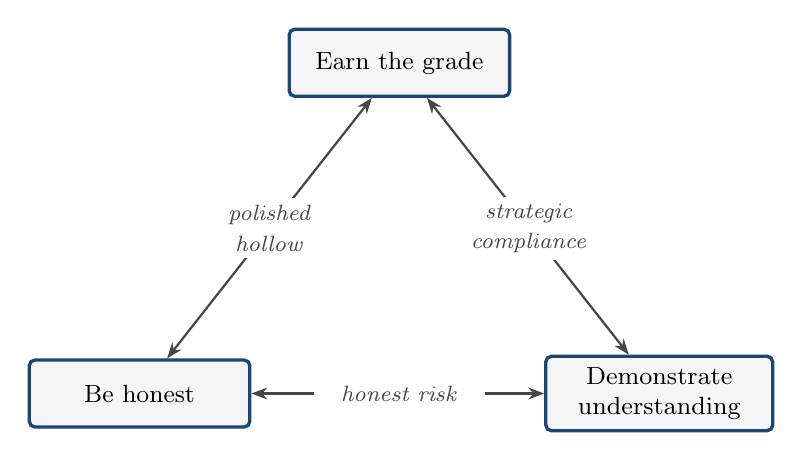
\begin{tikzpicture}
\node[emphasis-node, minimum width=2.8cm, minimum height=0.85cm, align=center]
  (grade) at (0, 2.8) {Earn the grade};
\node[emphasis-node, minimum width=2.8cm, minimum height=0.85cm, align=center]
  (honest) at (-3.3, -1.4) {Be honest};
\node[emphasis-node, minimum width=2.8cm, minimum height=0.85cm, align=center, text width=2.6cm]
  (understand) at (3.3, -1.4) {Demonstrate\\understanding};
\draw[bidir-arrow] (grade) -- (honest);
\draw[bidir-arrow] (grade) -- (understand);
\draw[bidir-arrow] (honest) -- (understand);
\node[caption-text, fill=white, align=center, text width=2cm, inner sep=2.5pt] at ($(grade)!0.5!(honest)$)
  {\footnotesize\textit{polished\\hollow}};
\node[caption-text, fill=white, align=center, text width=2cm, inner sep=2.5pt] at ($(grade)!0.5!(understand)$)
  {\footnotesize\textit{strategic\\compliance}};
\node[caption-text, fill=white, align=center, text width=2cm, inner sep=2.5pt] at ($(honest)!0.5!(understand)$)
  {\footnotesize\textit{honest risk}};
\end{tikzpicture}
% OVERFULL-BENIGN (S-alpha 2026-07-13): this figure is deliberately wider than the text block and
% page-centered; the two ~318pt overfull warnings are by design. Revisit only at SIAM production.
\caption{\textbf{The Student's Trilemma.} Three goals in genuine tension. Each edge labels the failure mode that arises when the two adjacent goals are satisfied at the cost of the third. The text develops the modes. AI sharpens each edge; it did not create the trilemma.}
\label{fig:honest-a-bind}
\end{figure}

The trilemma is not just one student's predicament. Recent surveys document how widely it is felt. The 2026 edition of the United Kingdom's Higher Education Policy Institute survey reports that 95\% of students now use AI in some form, up from 92\% in 2025 and 66\% in 2024, and that 94\% use it for assessed work \citep{stephenson2026student, hepi2025students}. A 2025 Inside Higher Ed Student Voice survey of more than a thousand students from 166 institutions found that students overwhelmingly want their institutions to address academic integrity through prevention rather than punishment \citep{insidehighered2025studentvoice}. A study of disclosure practices at King's Business School found that roughly three-quarters of students failed to declare AI usage even when instructed to do so, with the cited reasons including fear of negative perceptions and lower marks \citep{gonsalves2024addressing}. The trilemma names the structural predicament these numbers describe. AI use is widespread; honest disclosure is widely avoided; the gap between performance and underlying competence is widely felt but rarely acknowledged.

\subsection{Three student failure modes}
\label{subsec:trilemma-failures}%
\index{polished hollow!student}\index{strategic compliance!student}\index{honest risk!student}

\textit{Polished hollow.} The student earns the grade and discloses AI use honestly but cannot reproduce the work. The submitted artifact is fluent, organized, and correctly cited; the disclosure statement is candid; the underlying competence has not formed. The student does not necessarily realize this in the moment. They have read the AI's solution, found it convincing, and submitted it; what they have not done is reconstruct the steps themselves under conditions that would reveal the gap. The polished hollow is the failure mode that is invisible from outside and felt from inside. The student knows the work is hollow even when no one else does.

\textit{Strategic compliance.} The student earns the grade and genuinely understands the material but hedges on how AI helped. They used AI for first drafts, for clarifying confusing examples, for stress-testing their own arguments, for catching errors. The learning happened. But the account they give in disclosure statements is shaped to minimize what AI contributed, partly from expected suspicion and partly from inconsistent institutional signals about acceptable AI use. The disclosure is technically true and substantively misleading. Strategic compliance is the most common failure mode because it is the locally rational response to inconsistent expectations.

\textit{Honest risk.} The student is fully honest about both their AI use and the limits of their understanding. They disclose what they used AI for, what they verified independently, where they remain uncertain. Their work is documented and defensible. And they pay a competitive price for the transparency: the gradebook treats their disclosed AI-assisted draft the same as a peer's undisclosed identical draft, or worse if the disclosure prompts detector-driven suspicion. The student who refuses to play the strategic-compliance game pays the cost of refusing.

The three failure modes are not symmetric in their consequences. Polished hollow accumulates over time, hollowing out skill the student will eventually need. Strategic compliance protects the grade but corrodes the student's relationship with honest self-account. Honest risk costs the grade but preserves both competence and integrity. Different students under different pressures will find different modes locally least bad. The framework's value is not in telling students which mode to inhabit; it is in naming the structure so the choice is visible.

The three failure modes are also a tool for catching trouble early, while you work. If you could not rebuild the work without AI, you are sliding toward polished hollow. If you are shading how much AI actually helped, you are sliding toward strategic compliance. If staying honest is about to cost you the grade, you are sliding toward honest risk. When you notice one of these, the answer is not to give up that corner. It is to find the smallest change that restores it without letting the other two slip.

That works cleanly for two of the three. Rebuilding the work from a blank page restores understanding; disclosing fully restores honesty. Honest risk is the exception. When staying honest is what costs you the grade, the problem usually sits in the assignment or the grading, not in your own work. The smallest change that would fix it may not be yours to make. The responsible move there is to surface it rather than carry the cost alone: ask for clarification, an accommodation, an extension, or institutional help.

No fixed ranking works everywhere. The right balance depends on your situation, and it changes as the situation does.

\subsection{How the trilemma manifests differently for different students}
\label{subsec:trilemma-dimensions}

The trilemma is universal but its pull patterns are not. The three corners weigh differently depending on the student's situation. Four dimensions of variation matter most, and they are pressures that compound for individual students rather than discrete categories.

\textit{Economic stakes around the grade.} For a first-generation college student whose family is funding the degree as a generational investment, the grade carries weight that students from continuously-college-going families do not feel in the same way. Educational researchers have documented an AI digital divide along this dimension: first-generation students report lower awareness and use of generative AI tools than continuing-generation students, partly because of access constraints and partly because of weaker informal networks that pass on AI-use norms \citep{wgulabs2024divide}. The same student who would benefit most from AI literacy faces the trilemma's strategic-compliance edge most sharply, because the cost of the honest-risk failure mode is higher when the grade is more load-bearing.

\textit{Consequence severity around honest disclosure.} For an international student on an F-1 visa, an academic-integrity finding can trigger consequences far beyond the grade. Suspension or expulsion can terminate the student's SEVIS record and revoke their visa status, with departure or removal proceedings to follow. The honest-disclosure corner of the trilemma carries weight that domestic peers do not feel. The documented false-positive rate of AI-detection tools on non-native English writing (\cref{sec:disclosure}) compounds the pressure toward strategic compliance for students who can least afford an unfounded accusation.

\textit{Career stakes around demonstrated understanding.} For a pre-professional student preparing for medical school, law school, or competitive engineering programs, the credential's signaling value depends heavily on demonstrated independent capability. Polished-hollow work that produces high grades but weak underlying competence carries a delayed cost when the graduate enters a professional environment that tests them directly. The pre-professional student feels the polished-hollow edge of the trilemma most sharply, because the credential is being underwritten by future capabilities they have not actually built.

\textit{Time available for honest risk.} For working students, students with caregiving responsibilities, and other non-traditional students, the time required to make AI use sustainable (try first, verify independently, document the process, write transparent disclosures) competes directly with employment hours and family obligations. Strategic compliance is more often a structural condition than a chosen response for students whose lives leave no slack for the framework's full practice.

A single student often faces several of these pressures at once. A first-generation international pre-medical student who works thirty hours a week experiences all four. The framework's claim is not that this student should adopt some single right response, but that they should be able to see the structure they are responding to. You may see yourself in one of these pressures, or in several at once. The point is not to place yourself in a category. It is to recognize the pull you are actually under, so that what you do next is a choice rather than a reflex.

\subsection{What makes the trilemma hard to see}
\label{subsec:trilemma-invisibility}

The trilemma has a structural feature that makes it harder to address than most predicaments students face: \textbf{it is invisible to the people best positioned to remove it.} The polished hollow is designed to be invisible from outside; that is what makes it polished. The strategic-compliance hedge sounds plausible to instructors who are not asking detailed questions about it. The honest-risk price is paid silently, as a missing grade differential the student rarely raises because raising it would sound like a complaint.

Instructors designing courses and administrators setting policy often do not see the trilemma their students are navigating. The failure modes are structured to be unobservable from the instructor's vantage, and instructors and administrators face their own version of the same predicament (developed in Parts~\ref{part:instructor} and~\ref{part:institutional}). The framework's value to instructors and administrators is partly that it makes the student-side trilemma visible from the outside. The framework's value to students is that it names what they have been feeling without a vocabulary for it.

One direct counter-argument is worth taking seriously. A student interviewed in the same article that introduced Wendy asked the obvious question: \emph{If I am being asked to go from point A to point B, why wouldn't I use a car to get there?}\footnote{Quoted in \citet{walsh2025everyone}.} The honest answer is that the comparison fails because the road is the destination. The point of the homework is the walking, and the value of the walking is what the rest of this guide develops. The same is true in a different register for an essay, a problem set, or a research paper. The task that looks like a destination is usually a journey whose value lies in being travelled.

That qualifier matters, though. Not every task is a road worth walking. Some are errands, where the destination is the point and the walking is only transport, like reformatting a bibliography or converting a table from one format to another. So the judgment you need is which kind of task you face: is this path the competence the course exists to build, or incidental labor on the way to it? When the walking is the competence, do it yourself and let AI check it; when it is only transport, let AI carry it and spend your effort on what is actually the destination. Telling the two apart is itself one of the skills this guide teaches.

\subsection{Why the Student's Trilemma matters for the rest of Part I}
\label{subsec:trilemma-stakes}

The principles, practices, and tools developed in the rest of Part~\ref{part:student} are the operational response to the trilemma. The Learning Spiral in \cref{sec:learning-spiral} is designed to convert the honest-risk failure mode from a competitive disadvantage into a sustainable practice. The student who tries first, verifies, and works independently is producing the kind of evidence that makes honest disclosure defensible without paying the full price of polished-hollow protection. The CAT framework in \cref{sec:cat} aligns the three corners by separating what genuine competence requires (Core Competence), what responsible AI use looks like (AI-assisted Practice), and what trustworthy self-account involves (Trustworthiness). The translation test in \cref{sec:compact} is the diagnostic designed to catch polished-hollow work before it becomes a credentialing problem. The disclosure templates in \cref{sec:disclosure} are designed to make honest disclosure both possible and proportionate, reducing the structural pressure toward strategic compliance.

The same three-cornered framework applies in inverted forms to instructors and to institutions; Parts~\ref{part:instructor} and~\ref{part:institutional} develop the Instructor's Trilemma and the Institution's Trilemma respectively, with parallel failure modes and structural features. Students who recognize the trilemma in their own work will recognize the same structural pattern when their instructors and administrators describe their own predicaments. The pattern is the book's central structural claim, and Wendy's predicament is not unique to students.

\section{How learning happens, and how AI changes it}
\label{sec:learning-science}%
\index{learning science}\index{cognitive offloading}\index{productive struggle}\index{transfer}

Wendy's predicament has the shape it does because of how durable learning actually happens. The practices in this guide are not pulled from intuition. They are operational forms of principles from the science of learning that have been studied for decades. This short section names the principles, so the rest of Part~\ref{part:student} reads as application rather than assertion. The principles have a longer evidence base than the AI debates that frame them.

Five findings recur in studies of how durable learning happens.

\keyterm[practice testing]{Practice testing} (also called retrieval practice). Trying to recall information, or produce a solution, or reconstruct an argument, builds memory more strongly than re-reading or re-watching it \citep{roediger2006test}. The act of retrieval is itself a learning event, not just a check on what was already learned. The timing matters, and the result is instructive. In the study that established this, rereading won when the test came five minutes later. Testing won by a wide margin when the test came two days or a week later, and students were more confident after the method that lost. Most assessments measure production. Most studying measures recognition. The gap between them is one place where AI use is risky.

\keyterm[distributed practice]{Distributed practice} (also called spacing). Material reviewed at intervals, with forgetting and re-retrieval between sessions, is retained more durably than the same material reviewed in one block~\citep{dunlosky2013improving}. The interval is the work, not the wasted time. A short return to a problem one to three days later usually does more for memory than a long block on the day of first encounter.

\keyterm[interleaving]{Interleaving}. Mixed practice across problem types builds the discrimination skills that single-method practice does not \citep{rohrer2007shuffling}. Students who practice ten problems on the same method become fluent in that method. Students who practice ten problems mixing several methods become fluent at choosing which method applies. In mathematics and other quantitative disciplines, the second skill is often the one that matters on exams.

\keyterm[generation effect]{Generation effect}. Information that you produce is remembered better than information you read. Closing the AI window and rewriting the key step from memory is not a redundant exercise. It is the move that converts recognition into production.

\keyterm[desirable difficulties]{Desirable difficulties}. Conditions that slow initial performance, including productive struggle, retrieval failure, and effort to reconstruct, often produce more durable long-term learning \citep{bjork2011making}. Easy is not the same as effective. Fluent reading of a polished AI explanation is the easiest study experience available; it is rarely the most effective.

These five findings show up at specific places in the Learning Spiral introduced later in Part~\ref{part:student} (\cref{sec:learning-spiral}). \emph{Try to solve} uses retrieval practice and desirable difficulties. \emph{Verify} adds another retrieval pass and a chance for spaced and interleaved follow-up. \emph{Work independently} and the recommendation to redo key steps from a blank page rely on the generation effect. \emph{Reflect and disclose} closes the pass with elaboration and metacognition. Each step has a learning purpose, not just a procedural one.

\subsection{The illusion of competence}
\label{subsec:illusion}%
\index{illusion of competence}\index{metacognitive laziness}

A persistent finding in the science of learning is that students often think they understand material that they cannot actually reproduce, apply, or defend under questioning. I know the feeling from the other side of the lectern. As a student I listened to Richard Feynman lecture on physics and left each talk certain I had finally understood the subject. Hours later, trying to explain an idea to someone else, I found I could not reconstruct it. Many of my colleagues report the same experience with those lectures. The clarity was real, but it was recognition, not yet the ability to produce the argument myself. Feynman knew the trap, and named it in the line that opens this part: the easiest person to fool is yourself. The technical name for this gap is \keyterm{calibration error}: the distance between what you think you know and what you can demonstrate. Calibration error has been studied for decades. AI does not create the problem, but it can widen the gap in ways earlier study tools did not.

\begin{figure}[ht]
\centering
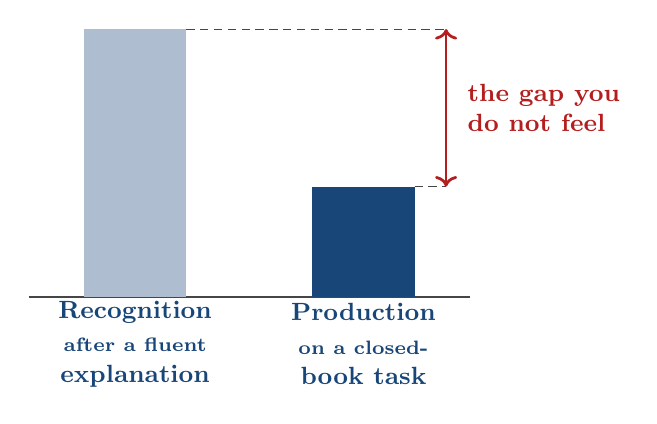
\begin{tikzpicture}
\draw[draw=darkgray, thick] (0,0) -- (5.6,0);
\fill[guideblue!35] (0.7,0) rectangle (2.0,3.4);
\node[font=\small\bfseries, color=guideblue, align=center] at (1.35,-0.6) {Recognition\\[1pt]\scriptsize after a fluent\\explanation};
\fill[guideblue] (3.6,0) rectangle (4.9,1.4);
\node[font=\small\bfseries, color=guideblue, align=center] at (4.25,-0.6) {Production\\[1pt]\scriptsize on a closed-\\book task};
\draw[densely dashed, darkgray] (2.0,3.4) -- (5.3,3.4);
\draw[densely dashed, darkgray] (4.9,1.4) -- (5.3,1.4);
\draw[<->, catNAI, line width=1pt] (5.3,1.4) -- (5.3,3.4);
\node[font=\small\bfseries, color=catNAI, anchor=west, align=left] at (5.45,2.4) {the gap you\\do not feel};
\end{tikzpicture}
\caption{\textbf{The recognition--production gap.} A fluent AI explanation produces a strong feeling of understanding (recognition), which can far outstrip what the same student can produce unaided on a closed-book task. The distance between the two is the calibration error a learner does not feel.}
\label{fig:recognition-production}
\end{figure}

The widening shows up in four places.

\emph{The recognition--production gap} (\cref{fig:recognition-production}). Reading a fluent AI explanation produces a strong feeling of understanding. That feeling is reliable for one thing: it tells you that you can recognize the explanation as correct when you see it again. It does not tell you that you can produce the explanation, or the underlying argument, on your own. Recognition memory and production memory are separate systems. AI delivers recognition. Assessments measure production. As one student put it, ``I read an AI proof, nodded along, then couldn't reproduce step two.'' The smoother the prose, the more carefully you should check the facts.

\emph{The mastery illusion on transfer}. After AI-assisted homework, students often predict they can solve similar problems independently on a quiz. The prediction is systematically wrong. Fluency on assisted work is a poor predictor of unassisted performance, especially when the new problem requires a small variation of method or a transfer to a new context~\citep{dunlosky2009metacognition}.

\emph{The effort illusion}. Time spent with AI feels productive. The hours register as study hours. But productive learning hours are hours in which you did the cognitive work: retrieval, reasoning, reconstruction, error repair. If AI did that work and you watched, the time is study time only in name.

\emph{The authorship illusion}. In extended AI-assisted writing or proof work, the line between ``I had this idea'' and ``AI suggested it'' can become difficult to track. The sensation that the work is yours grows even when most of the structure came from somewhere else.

These illusions are not failures of effort or honesty. They are predictable consequences of how memory, metacognition, and fluency interact \citep{bjork2011making,dunlosky2009metacognition}. The defense against them is not to avoid AI. It is to build in checks that reveal what you actually can do without it.

Most of the practices in this book are calibration checks. \emph{Try to solve} gets a baseline before AI flattens the picture. \emph{Verify} asks you to find errors in AI output, which requires that you understand the work. \emph{Blank-page redo} tests whether you can produce, not just recognize. \emph{Reflection and disclosure} track what you did versus what AI did. \emph{No-AI quizzes} and \emph{transfer questions} surface the gap between assisted and unassisted performance.

The instructor-side problem is parallel and is taken up at the start of Part~\ref{part:instructor}. Together, these checks, student-side and instructor-side, are what allow learning to remain visible in an environment where final products no longer reliably show how they were made.

\subsection{Calibration checks in the moment}
\label{subsec:calibration-checks-in-moment}

The four illusions develop slowly and become visible only when you try to do something new. Most students do not catch them in time, because the moment of catching is also the moment of submitting. The remedy is to build the catch into the work itself. Five short habits, run in the moment, do most of the work.

\emph{Predict before reading.} Before you read AI's next sentence, write down what step you expect next, or what conclusion you think it is heading toward. Then read. The gap between your prediction and AI's continuation is your calibration error, made visible at the granularity of one sentence. If the gap is large and surprising, you have learned something. If the gap is large and you find AI's reasoning hard to follow, you have learned that you are a step behind and need to slow down. The whole exercise takes ten seconds and converts passive reading into active hypothesis testing.

\emph{Forced unassisted gap.} After AI helps you with one problem, close AI and try the next problem of the same type without it. The drop in fluency between the assisted problem and the unassisted one is a rough probe of how much actually transferred. A small drop suggests the assisted work transferred. A large drop suggests you produced an answer without learning much. Most students do not run this check because the assisted problem feels finished and the unassisted one feels like extra work; that feeling is the effort illusion at work, and is what makes the check valuable.

\emph{Blank-page rehearsal.} At the end of each AI-assisted session, close AI, close your notes, and rewrite the key derivation, paragraph, or argument from a blank page. This is the strongest single calibration check available, because reconstruction from nothing tests production memory rather than recognition memory. The gap between your draft and what you can rebuild is the gap between recognizing the work and owning it. The student checklist in \cref{sec:student-checklist} ends with this item for the same reason.

\emph{Self-quiz on the next day.} Within twenty-four hours of an AI-assisted session, set yourself one question about what you worked on the day before, and answer it without the materials in front of you. This is retrieval practice on a one-day delay; it is also a calibration check, because the question reveals whether yesterday's understanding survived overnight. If it did not, you know to return to the topic before the next class or assignment.

\emph{Explanation aloud.} After any AI-assisted exchange, say out loud, in your own words, what you just learned. The act of vocalizing forces production. If you find yourself stalling, hedging, or reaching for AI's exact phrasing, you have caught a recognition--production gap in the act. The fix is to return to the underlying material, not to re-read AI's response.

These five moves are not a separate study program. They are micro-checks distributed across the Learning Spiral introduced later in Part~\ref{part:student} (\cref{sec:learning-spiral}), run as the work happens rather than at the end. \emph{Predict before reading} sits at the boundary between \emph{Ask} and the next AI turn. \emph{Forced unassisted gap} sits at the transition between \emph{Verify} and the next assignment. \emph{Blank-page rehearsal} runs at the close of \emph{Reflect}. \emph{Self-quiz} runs the day after, on the next pass. \emph{Explanation aloud} runs continuously, in any silence the work allows. Built into the work, calibration becomes a habit rather than a final exam.

These in-the-moment checks are real, but they are coarse, and they are weakest exactly where you most need them: when an illusion is strongest, the same judgment that produced it tends to rate the check as passed. Treat them as early warnings, not verdicts. The measures that do not run on your own judgment carry more weight. They include the structural checks later in this Part (units, limiting cases, an independent derivation, code that actually runs) and, above all, the work you produce under an instructor's no-AI assessment, the one signal these illusions cannot reach.

\section{The basic compact}
\label{sec:compact}%
\index{Student Compact}

AI-assisted learning works best when students and teachers share a clear compact.

You may use AI when your instructor allows it. You may ask it to explain ideas, question you, critique a draft, help you study, compare approaches, or point out possible weaknesses. You may use it as a tool for practice and improvement.

But when you submit work, the work is yours. That means you can explain it without saying, ``The AI told me.'' You know which sources support your claims. You understand the code you submit. You can describe how a paragraph changed during revision. You know what you accepted, what you rejected, and why.

This is not only an academic integrity rule. It is a learning rule. If you cannot explain the work, the work has not yet become part of your understanding.

One concrete diagnostic helps. Call it the \keyterm{translation test}: take a piece of work and re-present it in a different form. The broadest form of the test asks whether you can say the same thing three ways: visually (a picture, diagram, or graph), mathematically (with notation, equations, or formal structure), and in plain language (the kind of sentence you would use to explain the idea to a curious friend at dinner). A student who can move fluently between all three modes is showing ownership of the idea; a student who can perform only one likely has surface recognition, not structural understanding. The test has limits. Fluency can be rehearsed, and anxiety or an unfamiliar language can mask understanding a student really has, so treat a weak translation as a signal to look further rather than a verdict. The test measures whether you can move between forms, not how much you change the original. A draft you accept with few edits can still pass, provided you could re-present it in another form on demand. The point is portable understanding, not visible rework.

A specific case of the test is the notation change: rewrite the proof or argument using different variable names and symbols. \Cref{fig:translation-test} shows this form. The notation change is a useful diagnostic in mathematics and in any field that uses formal notation, but it is the narrowest version of the test. A student who can rewrite $f(x)$ as $g(t)$ has shown they recognize the structure under one specific kind of relabeling. On its own this is weak evidence: symbols can be swapped by pattern-matching without grasping what they mean. The relabeling has not shown the student could draw the same idea, or explain what is happening to someone who has never seen the notation. Treat it as the entry point to the test, not the test itself; the three-modality form catches both kinds of gap.

For non-mathematical work, the test usually runs on the plain-language axis. Paraphrase the passage in your own words, give the same example in a different form, or re-derive the result by a different route. The diagnostic is the same: fluent translation across modes indicates ownership; difficulty indicates recognition. The guide returns to this diagnostic throughout.

One limit is worth naming. The translation test fits understanding you can put into words and forms. Some competence you show by doing rather than describing; it lives in the performance itself, not in an account of it, and the instructor guide takes this up in \cref{i:subsec:skill}.
% DELIBERATE EXCEPTION (Mac, 2026-07-13): mathematical notation is allowed in this figure and its
% caption, overriding the Part I no-notation rule. The figure is about renaming symbols; the
% notation is load-bearing. Do not "fix" this under the accessibility rule.
\begin{figure}[ht]
\centering
\small
\begin{tabular}{p{0.42\textwidth} p{0.42\textwidth}}
\textbf{\textcolor{guideblue}{Original notation}} &
\textbf{\textcolor{guideblue}{Translated notation}} \\[0.2em]
\multicolumn{2}{c}{\footnotesize\textit{Renaming:}\; $M \to B$,\quad $x \to t$,\quad $f \to g$,\quad $x^* \to t^*$} \\[0.4em]
\hline \\[-0.5em]
$M = \sup_{x \in [0,1]} f(x)$ & $B = \sup_{t \in [0,1]} g(t)$ \\[0.5em]
$\exists\;x_{n_k} \to x^* \in [0,1]$ (Bolzano--Weierstrass) & $\exists\;t_{n_k} \to t^* \in [0,1]$ (Bolzano--Weierstrass) \\[0.5em]
$f(x^*) = M$ by continuity & $g(t^*) = B$ by continuity \\[0.3em]
\hline \\[-0.3em]
\multicolumn{2}{c}{\normalfont\textit{If you can write the right column fluently, the proof is yours.}}
\end{tabular}
\caption{\textbf{The translation test in practice.} Fluency in the right column is the test: if you can write the translated argument as easily as the original, your understanding lives in the argument's structure rather than in its symbols. The renaming line under the headers carries the whole change; nothing else differs between the columns. To run the test on yourself, cover the left column and rebuild the right one from the renaming alone.}
\label{fig:translation-test}
\end{figure}

The translation test catches more than single-chat overreliance. It also catches AI work produced outside any single, identifiable session, including work whose surface was polished in one chat while the actual content was drafted in another. The test asks what the student can do regardless of which chat produced what. The operational version of this concern is treated in \cref{subsec:thread-sharing}; the translation test is the structural safeguard that does not depend on which chat is shared.

The compact has five parts.

\begin{description}
\item[Attempt.] Try the task before asking AI to do anything important.
\item[Use.] Ask AI for support that keeps you active.
\item[Verify.] Check important claims, sources, computations, and interpretations.
\item[Disclose.] State how AI was used when the assignment requires it.
\item[Own.] Submit only work you can explain and defend.
\end{description}

Different courses will apply this compact in different ways. A professor may ban AI on an exam, allow it for practice, require it for a critique assignment, or ask you to compare your answer with an AI answer. The exact rule belongs to the course. The responsibility belongs to you. With AI tools the habit is easy to state and hard to keep: verify, verify, verify, then trust.

Some courses adopt the compact as a signed agreement between student and instructor. A signature line is included here for that use; a printable one-page copy is in the repository (\texttt{companion/compact/}).

\bigskip
\noindent Signed: \rule{5.5cm}{0.4pt} \hfill Date: \rule{3.2cm}{0.4pt}

\chapter{The Framework}
\label{ch:the-framework}%

\bookepigraph{AI does not prevent mistakes.\\It lowers the cost of making, examining, and learning from them.}

\section{The CAT framework}
\label{sec:cat}%
\index{CAT framework}

This guide uses the CAT framework: \keyterm[CAT framework!Core Competence]{Core Competence}, \keyterm[CAT framework!AI-assisted Practice]{AI-assisted Practice}, and \keyterm[CAT framework!Trustworthiness]{Trustworthiness}. These three dimensions help you understand what your instructor may be trying to assess. Trustworthiness is the one most often misread. It is not a judgment about your character. It scores what you did: whether you verified the work, said how it was made, and can answer for it. A student who does not disclose may simply never have been shown how, and the axis should read that as missing instruction rather than missing honesty. Graduate students whose programs use the original three-axis framework will find the technical version, and its original names, in Appendix~\ref{app:gmip}. The substance is the same.

\subsection{Core Competence}
\label{subsec:core-competence}

Core Competence is what you must be able to do without AI, or with only tightly limited help. Every course has a core. In chemistry, it may include explaining mechanisms and interpreting lab results. In writing, it may include building an argument and revising a draft with intention. In history, it may include reading sources carefully. In mathematics, it may include solving problems and explaining definitions. In programming, it may include tracing code and debugging simple errors.

AI does not remove the need for these abilities. It makes them more important. If a tool can generate a fluent answer, your value as a learner comes from knowing whether the answer is right, relevant, honest, and useful.

There is a useful way to see why. Tools that help us think divide into two kinds \citep{norman1991cognitive,krakauer2016hybrid}. Some we can internalize. A student who practices with an abacus or with written place value eventually carries the method in their head and can set the tool aside. The tool leaves a durable skill behind. Others work only while they are switched on. A calculator or a car's navigation gives a correct result and teaches nothing that survives its removal, and long reliance can leave the underlying skill weaker than before. The first kind builds capability. The second kind rents it. Whether AI becomes one or the other is not decided by the tool. It is decided by how a course asks students to use it \citep{bowen2024teaching,watson2024learning}. An assignment that asks for the answer trains dependence. An assignment that asks the student to attempt the reasoning first, then use AI to check it, uses the same tool to build a skill the student keeps.

Expect some assignments to test Core Competence directly. These may include no-AI quizzes, in-class writing, lab practicals, oral explanations, short exams, source analyses, board work, or live coding checks. These assessments are not a rejection of AI. They protect the part of learning that must remain yours.

\subsection{AI-assisted Practice}
\label{subsec:ai-augmented-practice}

AI-assisted Practice is your ability to use AI well. This is also a real skill. It includes asking useful questions, judging responses, comparing explanations, finding weak points, generating practice problems, revising carefully, testing code, checking assumptions, and using feedback without becoming dependent on it.

Good AI use is not measured by how much AI contributed. It is measured by whether AI helped you think better.

A weak use of AI is asking for a complete solution and copying it. A stronger use is asking for a hint, trying the next step yourself, and then checking whether your reasoning holds. A weak use of AI is asking it to write a paper. A stronger use is asking it to find the least convincing paragraph in your own draft and explain why a reader might not believe it.

You can practice the conversion directly. Take the last question you actually asked an AI and rewrite it two ways: once so the AI must give you a hint rather than a solution, and once so it must critique work you supply rather than produce work for you. For example:

\studentprompt{I am stuck on [problem]. Do not give me the solution. Ask me one question that would help me find my own next step.}

\studentprompt{Here is my draft paragraph: [paste]. Find the weakest claim and explain why a careful reader would doubt it.}

Chapter 4 practices this conversion across the common use cases.

\subsection{Trustworthiness}
\label{subsec:responsible-judgment}

Trustworthiness is your ability to verify, disclose, critique, and take ownership of \keyterm{AI-assisted work}: work shaped in some way by an AI tool, including brainstorming, drafting, revision, coding, explanation, summarization, critique, or feedback. This is the ethical center of the guide.

Trustworthiness asks practical questions.

\begin{itemize}
\item Did I check whether the AI response is true?
\item Did I verify sources rather than trusting generated references?
\item Did I protect private or restricted information?
\item Did I disclose AI use when required?
\item Can I explain what I submitted?
\end{itemize}

One more question turns inward. Trustworthiness includes self-calibration: knowing whether you actually understand the work, or whether it only looks right to you. The illusion of competence in \cref{sec:learning-science} makes this the easiest judgment to get wrong, and a fluent AI answer makes it easier still. The same tool can help you check: ask it to quiz you on the parts you are least sure of, or to find the step you could not reproduce on your own. Being trustworthy to others starts with an honest account of what you know.

The best-practice norms for ethical AI-assisted scientific writing (Appendix~\ref{app:sciwriting}) state the same principle in a research setting: AI assistance becomes acceptable only when the human author verifies the content and accepts responsibility for it. The guide applies that principle to student learning. AI may assist, but the final responsibility is yours.

\subsection{Relation to international AI competency frameworks}
\label{subsec:cat-unesco}%
\index{UNESCO AI competency framework}

The CAT framework is narrower in scope than the UNESCO AI competency framework for students \citep{miao2024aia}, which articulates twelve competency blocks across four aspects (Human-centred mindset, Ethics of AI, AI techniques and applications, AI system design) and three progression levels (Understand, Apply, Create). UNESCO addresses what every citizen should know about AI in society. CAT addresses something narrower: how a student demonstrates that submitted academic work reflects their own understanding when AI tools are available. The two frameworks complement each other. CAT is best understood as a focused subset of UNESCO's broader competency map applied specifically to the assessment of academic work.

\Cref{tab:cat-unesco} sketches the correspondence. Core Competence overlaps most strongly with the discipline-specific knowledge a student demonstrates within UNESCO's \emph{AI techniques and applications} aspect at the \emph{Apply} level, but extends beyond AI competence into the discipline's own foundational skills. AI-assisted Practice corresponds most closely to UNESCO's \emph{Apply} level across all four aspects. Trustworthiness maps onto UNESCO's \emph{Human-centred mindset} (specifically Human accountability) and \emph{Ethics of AI} (specifically Safe and responsible use). The mapping is not one-to-one because the frameworks were designed for different purposes. But a student or program that has met UNESCO's competency expectations will already have done much of what CAT asks for.

\begin{table}[ht]
\centering
\caption{\textbf{CAT and the UNESCO student framework.} The book's categories are not invented in isolation. They line up with UNESCO's competency framework \citep{miao2024aia}. The correspondence is partial by design. UNESCO covers AI literacy and AI design across a student's whole education. CAT answers one narrower question, what a piece of submitted work is allowed to contain, and answers it sharply enough to write on a syllabus.}
\label{tab:cat-unesco}
\begin{tabularx}{\textwidth}{>{\raggedright\arraybackslash}X >{\raggedright\arraybackslash}X}
\toprule
\textbf{CAT component} & \textbf{Closest UNESCO competency blocks} \\
\midrule
Core Competence & Discipline-specific foundations; partial overlap with AI foundations and Application skills (\emph{Understand} and \emph{Apply} levels of \emph{AI techniques and applications}). \\
\addlinespace
AI-assisted Practice & The \emph{Apply} level across all four UNESCO aspects, especially Application skills under \emph{AI techniques and applications}. \\
\addlinespace
Trustworthiness & Human accountability (\emph{Apply} of \emph{Human-centred mindset}); Safe and responsible use (\emph{Apply} of \emph{Ethics of AI}); Embodied ethics (\emph{Understand} of \emph{Ethics of AI}). \\
\bottomrule
\end{tabularx}
\end{table}

The framework's positioning relative to UNESCO matters for adoption. A program that already aligns its curriculum with UNESCO's framework can adopt CAT as the assessment-level operationalization of UNESCO's expectations for AI-assisted academic work, without abandoning the broader UNESCO structure.

\section{The Learning Spiral}
\label{sec:learning-spiral}%
\index{Learning Spiral}

The Learning Spiral is the main habit this guide asks you to practice, and it begins with a question. Framing a clear question is the move the whole practice turns on, which is why it sits at the center of the spiral (\cref{fig:learning-spiral}). Around that question run five steps: try to solve, ask for help, work independently, verify, and reflect. The Spiral assumes you have already set up your AI account, so the tool knows who you are and how you want it to respond. If you have not, do that now with the starter template in \cref{sec:setup}. The Spiral depends on it. The five steps recur on every AI-assisted task, and each pass should deepen what you understand rather than return you to where you began. A question is not finished when you answer it. Pursued well, it opens a deeper question, and the spiral widens. This is why the framework is a spiral rather than a loop.

\begin{figure}[ht]
\centering
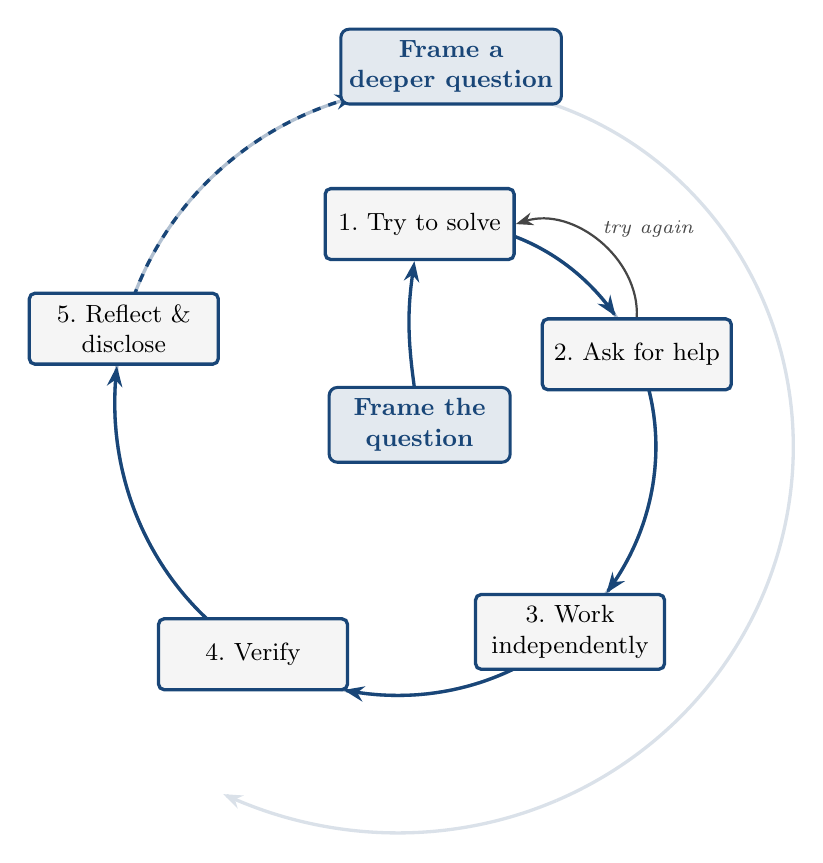
\begin{tikzpicture}
% faint spiral underlay through the box centers, plus the never-closing continuation
\draw[guideblue!34, very thick, domain=90:-285, samples=320, smooth, variable=\t]
  plot ({(2.55 + 0.35*((90-\t)/72))*cos(\t)}, {(2.55 + 0.35*((90-\t)/72))*sin(\t)});
\draw[guideblue!16, very thick, domain=-285:-430, samples=160, smooth, variable=\t]
  plot ({(2.55 + 0.35*((90-\t)/72))*cos(\t)}, {(2.55 + 0.35*((90-\t)/72))*sin(\t)});
\draw[guideblue!16, very thick, -{Stealth[length=2.4mm]}, domain=-430:-478, samples=70, smooth, variable=\t]
  plot ({(2.55 + 0.35*((90-\t)/72))*cos(\t)}, {(2.55 + 0.35*((90-\t)/72))*sin(\t)});
% bold arrows are segments of the same spiral, drawn before the boxes so each box covers the
% inner end of its own arrow; each head is trimmed to land on the next box's side
\draw[emphasis-arrow, domain=90:29,    samples=80, smooth, variable=\t]
  plot ({(2.55 + 0.35*((90-\t)/72))*cos(\t)}, {(2.55 + 0.35*((90-\t)/72))*sin(\t)});
\draw[emphasis-arrow, domain=18:-42,   samples=80, smooth, variable=\t]
  plot ({(2.55 + 0.35*((90-\t)/72))*cos(\t)}, {(2.55 + 0.35*((90-\t)/72))*sin(\t)});
\draw[emphasis-arrow, domain=-54:-106,  samples=80, smooth, variable=\t]
  plot ({(2.55 + 0.35*((90-\t)/72))*cos(\t)}, {(2.55 + 0.35*((90-\t)/72))*sin(\t)});
\draw[emphasis-arrow, domain=-126:-191, samples=80, smooth, variable=\t]
  plot ({(2.55 + 0.35*((90-\t)/72))*cos(\t)}, {(2.55 + 0.35*((90-\t)/72))*sin(\t)});
% reflection opens a deeper question; the dashed segment continues the spiral outward
\draw[emphasis-arrow, dashed, domain=-198:-259, samples=80, smooth, variable=\t]
  plot ({(2.55 + 0.35*((90-\t)/72))*cos(\t)}, {(2.55 + 0.35*((90-\t)/72))*sin(\t)});
% central question
\node[seed-node] (frame) at (0,0) {Frame the\\question};
% five steps spiraling outward from the question
\node[emphasis-node, minimum width=2.4cm, minimum height=0.9cm] (try)    at (0,2.55)        {1.~Try to solve};
\node[emphasis-node, minimum width=2.4cm, minimum height=0.9cm] (ask)    at (2.758,0.896)   {2.~Ask for help};
\node[emphasis-node, minimum width=2.4cm, minimum height=0.9cm] (work)   at (1.910,-2.629)  {3.~Work\\independently};
\node[emphasis-node, minimum width=2.4cm, minimum height=0.9cm] (verify) at (-2.116,-2.913) {4.~Verify};
\node[emphasis-node, minimum width=2.4cm, minimum height=0.9cm] (reflect)at (-3.757,1.221)  {5.~Reflect \&\\disclose};
% the regenerated, deeper question one turn out
\node[seed-node] (framenext) at (0.40,4.55) {Frame a\\deeper question};
% launch from the question
\draw[emphasis-arrow] (frame) to[bend left=8] (try);
% the try-ask loop: a hint goes back into a new attempt (arc one rank below the main path)
\draw[-{Stealth[length=2.2mm]}, thick, draw=darkgray] (ask.north) to[bend right=55] node[midway, above right, inner sep=1pt, font=\scriptsize\itshape, text=darkgray]{try again} (try.east);
\end{tikzpicture}
\caption{\textbf{The Learning Spiral.} Five steps around a question at the center: try to solve, ask for help rather than for a solution, work independently, verify, and reflect. The spiral widens rather than closing into a loop, because a question pursued well opens a deeper one. That is what makes this a spiral and not a cycle, and the dashed arrow marks the opening. Each step earns its place: trying before asking protects independent thinking, working independently after the help is what confirms you understood it, verification catches errors, and reflection closes the pass. The small return arrow between steps 2 and 1 marks the loop to expect in practice: try, ask, and try again until the idea holds, and only then work independently.}
\label{fig:learning-spiral}
\end{figure}

Read as a rubric, those same five steps become what AI-assisted work should show (\cref{i:sec:cat-framework}).

% Deliberate inline-table idiom (unnumbered, uncaptioned); also used at B.4 and C.6. Keep unnumbered in production.
\begin{center}
\begin{tabular}{>{\bfseries}p{0.18\textwidth}p{0.75\textwidth}}
\toprule
Step & What it means \\
\midrule
Try to solve & Make an honest attempt before asking AI for help. \\
Ask for help & Ask for hints, explanations, questions, feedback, or critique. \\
Work independently & Return to the task and produce your own answer, draft, code, or analysis. \\
Verify & Check important claims, sources, computations, and assumptions. \\
Reflect and disclose & Record what AI contributed, what you changed, and what you can now explain. \\
\bottomrule
\end{tabular}
\end{center}

The spiral runs at multiple time scales. Within a single task the steps keep their order, but the first two form a loop: try, ask, and try again until the idea holds. Only then does the work go independent. The later steps can send you back as well: a failed verification returns you to asking, and an explanation you cannot finish returns you to the material. The figure draws only the loop that runs most often. Across an assignment, a unit, or a semester, the spiral repeats and widens. What you learned from verifying one pass becomes part of your first attempt in the next. What you reflected on becomes the question that opens the next round. The work on each task feeds a longer arc of deeper questions across the course.

The five steps name skills, not behaviors that come automatically. A first-generation student new to a discipline may not know what a first attempt looks like for a proof, what verifying means for a citation in a specific field, or what counts as working independently in a programming class versus a literature class. Each step is a skill to be built, often in partnership with an instructor, advisor, or the study practices the rest of this Part describes. If you recognize yourself in this paragraph, the framework was built with your starting point in mind. The companion materials in \texttt{companion/spp/} support students who are new to any of this.

\subsection{Frame the question}
\label{subsec:frame-question}%
\index{Learning Spiral!frame the question}

Every pass through the spiral starts with a question. Sometimes the assignment hands you one. More often the real question is yours to find: what are you actually trying to understand, and what is the part you cannot yet do? Framing that question well is the move the rest of the spiral depends on, because a vague question pulls a vague answer out of any tool, while a sharp one tells you what kind of help you need.

A good question names what you want to know and where your understanding stops. Putting a confusion into words is itself a way of learning, because it forces you to organize what you already know and to locate the edge of it. This kind of self-questioning is close to what learning research calls self-explanation, which has good support as a study habit \citep{dunlosky2013improving}. Before you reach for AI, write the question down in your own words.

Sometimes you open the assignment with no idea where to begin, often because the topic is new and you have not had a chance to prepare. This is common in your first courses, and it does not mean you cannot do the work. It means framing needs a step in front of it, because you cannot ask a useful question about material you have not met yet. Spend a few minutes meeting it. Skim the section, the problem, or the reading for its shape: what is this about, what are its main pieces, and what is it asking you to produce? You are not trying to understand all of it. You are trying to find the one place where you first get lost, the first sentence or step you cannot follow. That turns ``I do not understand any of this'' into ``I do not understand this part,'' which is a question you can work with. As a practical threshold, give yourself five to ten minutes to find the shape of the material and the point where you get lost.

A question rarely ends where it starts. As you work through it you will understand more, and that understanding will raise a sharper question than the one you began with. The spiral widens because answering a question well is what shows you the next one.

A few moves help you find that next question. Ask whether your answer holds beyond this case, what made it work, where it breaks, whether it runs the other way, and whether you can sharpen it. Each of these turns an answer into a better question, and one is enough to begin the next pass.

\subsection{Try to solve}
\label{subsec:try-first}%
\index{Learning Spiral!try to solve}

Before using AI, make a first attempt. Write down what you think the problem asks. Draft a paragraph. Sketch the argument. Try the calculation. Read the primary source. Mark the confusing sentence. Run the code. List the assumptions.

This first attempt does not need to be good. Its purpose is to give your mind something to work with. Once you have tried, AI can help you compare, clarify, and repair. Without that first attempt, AI is more likely to become a substitute for thinking.

A counterintuitive finding in the learning literature is that effortful generation, including unsuccessful generation, often produces more durable memory than studying correct examples alone~\citep{bjork2011making,kornell2009unsuccessful}. Even when your first attempt is wrong, the act of attempting before consulting AI strengthens what you will learn from AI's response. That benefit depends on the feedback arriving: a failed attempt that is never resolved teaches little.

A recent MIT study makes the same point. Researchers watched students' brains during essay writing under three conditions: no tools, a search engine, and an AI assistant. Minutes after finishing, the AI-assisted writers struggled to quote their own essays. Students who wrote without AI remembered far more. The recordings suggest why. Students who started with the AI shifted from generating their own content to supervising the machine's, and their overall neural connectivity dropped. A smaller follow-up session pointed the same way. Students who wrote alone first and then turned to AI kept higher recall and engagement than those who started with AI \citep{kosmyna2025brain}. Read all of this as provisional. It is a preprint, and other researchers have raised questions about its sample size and analysis \citep{stankovic2026comment}. The pattern matches the rule above, and the rule does not depend on it: the first attempt gives your mind something to work with, and later AI assistance amplifies that effort rather than replacing it.

As a practical threshold: for routine homework, give yourself at least ten to fifteen minutes of serious attempt before asking AI for a hint. For a proof or open-ended problem, spend enough time to write down the definitions, the goal, one possible strategy, and the point where you are stuck. Do not ask AI before you have something for it to respond to.

\subsection{Ask for help, not replacement}
\label{subsec:ask-for-help}%
\index{Learning Spiral!ask for help}\index{help, asking for!going backward}

A useful AI question keeps you active. It asks for support that leaves the central thinking with you.

\index{escalation of AI requests}\index{help, asking for!escalation}The requests that replace your work are rarely the first ones a student makes. They are where a session ends up, usually late, usually on a night when one problem is still open and the clock is not. The route there is worth seeing, because every step on it is reasonable and none of them feels like a decision.

It starts with a real question. Twenty minutes in and stuck at the setup, a student asks where the problem begins. The answer helps, and they move. A few lines later the next obstacle arrives, and they ask whether the method they chose is the right one. Still fine. Then they have a setup on the page and ask the AI to check it, which is the first request that hands over a judgment instead of asking for help making one. Then they ask for the first two steps and promise themselves the rest. Then they ask for the answer.

The tell is not the wording of the prompt. It is what the student made between one prompt and the next. Early on they were making attempts. Later they were only making decisions about the AI's work. At the end they were making nothing, and the page was finished and not theirs.

One question catches this, and you have to ask it before you type: what have I produced since the last time I asked? If the honest answer is nothing, you have already moved, and the next request will move you further than it looks. The last stop on that road is the first prompt below.

Instead of asking:

\studentprompt{Write my answer to this problem.}

try asking:

\studentprompt{Give me one hint about how to start, but do not solve the problem.}

Instead of asking:

\studentprompt{Write my essay on this topic.}

try asking:

\studentprompt{Here is my thesis and outline. What is the weakest part of the argument?}

Instead of asking:

\studentprompt{Fix my code.}

try asking:

\studentprompt{Ask me diagnostic questions that would help me locate the bug.}

A different kind of help is useful when the trouble is not a problem you are solving but an idea you cannot get into focus. When a concept sits above your current level, ask for it three ways at once: as a plain analogy, at your working level, and one step deeper than you are now. Instead of asking:

\studentprompt{Explain this concept.}

try asking:

\studentprompt{Explain this concept three ways: first with an everyday analogy, then at the level of someone taking this course, then one step more advanced so I can see where it leads.}

The three levels give you an entry point, a working understanding, and a direction, and the gaps between them are often where the idea finally clicks. This is a strong way to get unstuck on difficult reading, and it comes with the same catch as every other step in the spiral: a clear three-level explanation can feel like understanding without being it. The explanation has done its work only when you can close the window and rebuild the idea in your own words. Students who want a tested prompt for this can use the layered-explanation template in the companion repository (\texttt{companion/layered-explanation/}).

The best prompts are not commands to replace your work. They are requests for coaching. Good help sometimes goes backward before it goes forward. If a hint keeps missing, the problem may rest on an idea you have not firmly grasped, and the quickest way through is to step back to that idea, make it solid, and climb back to the question. Students who want a tested prompt for converting the AI into a study partner rather than an answer machine can use the Study Partner Protocol (SPP) in the companion repository (\texttt{companion/spp/}). A hint is not the end of the exchange. Take it back to the problem and try again, and ask again if the new attempt stalls. Most of the learning happens inside this loop. Working independently begins when the loop ends, when you can rebuild the work with the AI closed.

\subsection{Work independently}
\label{subsec:work-independently}%
\index{Learning Spiral!work independently}

After receiving help, step away from the AI response and do the work yourself. Write the paragraph in your own words. Complete the proof or calculation. Revise the code. Rebuild the argument. Explain the source. Decide what belongs in the final submission.

This step is easy to skip because AI output often looks finished. Do not confuse finished-looking with learned.

A good test is simple: close the AI window and try to explain the idea aloud. If you cannot explain it, return to the material.

\subsection{Verify}
\label{subsec:verify}%
\index{Learning Spiral!verify}

\keyterm{Verification} is the act of checking AI-assisted content against reliable evidence, sources, data, tests, methods, or reasoning. It is the habit that turns AI assistance into responsible academic work. It is also the most important calibration check in the Learning Spiral: finding errors in AI output requires that you understand the work well enough to recognize when something is wrong. AI systems can produce confident errors. They can invent sources, misread prompts, use the wrong method, make hidden assumptions, or change the meaning of your sentence.

It is worth knowing why the errors arrive dressed as confidence, because the reason is not a flaw someone forgot to fix. \index{Kalai hallucination analysis}Kalai and colleagues trace it to two causes.

Some facts cannot be learned from the training data at all. A fact that appears once, or never, leaves no pattern to generalize from, so errors on questions of that kind are expected rather than surprising. That explains the wrongness. It does not explain the certainty.

The certainty comes from how these systems are graded. Most of the tests used to rank them score an answer right or wrong and award nothing for saying ``I do not know.'' Under that rule a guess is always worth more than an admission of uncertainty, so a system trained against those tests learns to answer as though sure \citep{kalai2025hallucinate}. The posture is the one a student learns under the same incentive. On an exam that gives no credit for a blank, bluffing beats leaving it empty.

The practical consequence is short. Confidence carries no information about correctness. It was never trained to.

Verification looks different in different fields; \cref{sec:verification} works the checks discipline by discipline, and \cref{fig:verification-disciplines} summarizes them at a glance. The details vary. The standard does not: do not submit AI-assisted work until you have checked the parts that matter, until you can explain why the answer is right and not merely confirm that it looks right. The AI answer is a draft, not a witness. An outside check is worth most exactly where your own sense of the answer is weakest, which is where a confident illusion is hardest to catch from the inside.

Where possible, return to the same problem type, or a mixed set of related problem types, one to three days later without AI. This spaced and interleaved retrieval is what converts a single working session into durable understanding \citep{rohrer2007shuffling}. Verification confirms that you understood the work today. Spaced and interleaved practice confirms that you will still understand it next week.

\subsection{Reflect and disclose}
\label{subsec:reflect-disclose}%
\index{Learning Spiral!reflect and disclose}

Reflection helps you notice what you learned. Disclosure helps your instructor understand how the work was produced.

To make reflection concrete, after each AI-assisted session answer in your own words: Why does each step in this proof, solution, or argument work? What would change if one assumption were weakened or removed? These two questions take thirty seconds and turn the session into elaborative practice. A useful weekly habit is to schedule two or three short interleaved retrieval sessions using your hard-problems list or verification checklist. The pattern is short, mixed, and unassisted.

When disclosure is required, use clear and ordinary language. You do not need to apologize for allowed AI use. You do need to be honest.

A good disclosure block looks like this:

\begin{quote}
\textbf{Tools used:} I used an approved AI tool.\\
\textbf{Tool role:} I used it to generate practice questions and critique my draft introduction.\\
\textbf{What I accepted or changed:} I used two suggested questions, but rewrote the introduction myself.\\
\textbf{Verification:} I checked the factual claims against the assigned reading and removed one unsupported claim.\\
\textbf{What I can explain:} I can explain the final thesis, evidence, and revision choices without AI.
\end{quote}

Some courses will require more detail. Some will require none for minor uses. Follow the assignment instructions. When an instructor asks to see the AI conversation itself, thread sharing (\cref{subsec:thread-sharing}) is the most direct disclosure available. For most AI-assisted work it makes the written block unnecessary.

\section{Four assignment categories}
\label{sec:assignment-categories}%
\index{assignment categories}\index{traffic-light metaphor}\index{assignment categories!No AI (NAI)}\index{assignment categories!AI as Tutor (AIT)}\index{assignment categories!AI as Collaborator (AIC)}\index{assignment categories!AI as Object of Study (AIS)}

Each assignment should tell you what kind of AI use is allowed. When the instructions are unclear, ask before using AI in a way that affects submitted work.

Instructors increasingly mark their assignments with one of four short labels that signal how AI fits the learning goal. The labels are color-coded. The colors carry meaning. Three of them sit on a traffic light:

\begin{itemize}
\item \NAI{} (No AI): red. Stop. The assignment measures what you can do without assistance.
\item \AIT{} (AI as Tutor): yellow. Proceed with care. AI may coach you toward understanding, but the submitted work must be yours.
\item \AIC{} (AI as Collaborator): green. Go. AI may co-produce work with you, and the assignment treats the collaboration as part of the learning.
\end{itemize}

The fourth label is a different kind of sign:

\begin{itemize}
\item \AIS{} (AI as Object of Study): blue. Off the traffic light entirely. The question is not how much AI you may use but what AI is doing: you study AI itself rather than using it as a tool.
\end{itemize}

\NAI{}, \AIT{}, and \AIC{} vary along one axis: how much AI freedom the assignment allows. \AIS{} is not a point on that axis. It is a different question altogether, which is why it gets a different color.

\subsection{\texorpdfstring{\NAI{}: No AI}{NAI: No AI}}
\label{subsec:red}

In an \NAI{} assignment, AI use is not allowed. The purpose is to measure what you can do independently.

Examples include closed-book exams, short quizzes, in-class writing, oral explanations, lab practicals, live coding checks, language drills, or foundational calculations.

An \NAI{} assignment is not a claim that AI is bad. It is a way to protect Core Competence. You need some abilities that do not depend on a tool being open in another window.

\subsection{\texorpdfstring{\AIT{}: AI as Tutor}{AIT: AI as Tutor}}
\label{subsec:yellow}

In an \AIT{} assignment, AI may be used for study support, but not to produce submitted work. What sets the category is where the AI's work ends up, not how well you understand it. If you write or work out the submission yourself, with no AI-generated text, code, or solutions carried into it, the assignment stays \AIT{}. Once AI's wording, code, or worked solution becomes part of what you hand in, the work has crossed into \AIC{} territory, which is a different category with different rules. If the analysis or the argument is AI's, putting it in your own words leaves the work \AIC{}. Whether you could reproduce that work from your own understanding is a separate question. That is the ownership question, and the translation test is how you check it. Understanding is what makes \AIC{} work honest. It does not turn it back into \AIT{}.

You may ask AI to explain a concept, quiz you, give hints, make flashcards, create practice problems, or help you prepare for class. You should not ask it to write the final answer.

\AIT{} use is common when the instructor wants you to learn from AI without letting AI shape the submitted product. The Study Partner Protocol (SPP) in the companion repository (\texttt{companion/spp/}) is designed for exactly this kind of AIT work. When \AIT{} work produces a tutoring conversation worth showing your instructor, thread sharing (\cref{subsec:thread-sharing}) documents the interaction more cleanly than any written summary.

The protocol's opening lines set the pattern:

\begin{quote}\small\textsf{For this conversation, act as my study partner, not an answer service. Your goal is to help me learn, so I should end up able to do the work myself. Before helping with a problem, ask me what I have already tried and where I am stuck. If I have not tried yet, ask me to make a first attempt before you help. Give hints, ask guiding questions, and point to the relevant idea. Do not give full solutions, finished proofs, or final written answers unless I explicitly ask for a worked example after trying. When I think I understand, ask me to explain it back in my own words, and check my explanation. If I ask you to just give me the answer, remind me once of this arrangement, then respect my choice.}\end{quote}

The full protocol, including the course-scope and step-back rules, is in the repository (\texttt{companion/spp/}).

\subsection{\texorpdfstring{\AIC{}: AI as Collaborator}{AIC: AI as Collaborator}}
\label{subsec:green}

In an \AIC{} assignment, AI may help with brainstorming, drafting, debugging, revision, critique, outlining, coding, or comparison. You must still verify the result and disclose AI use when required.

\AIC{} assignments are useful when the learning goal includes process, revision, research, modeling, design, computation, or professional practice. The instructor is not only asking what you know. They are also asking whether you can use tools responsibly. Because the AI's contribution is part of what is being assessed, thread sharing (\cref{subsec:thread-sharing}) is often the most natural way to disclose how the work was produced.

\subsection{\texorpdfstring{\AIS{}: AI as Object of Study}{AIS: AI as Object of Study}}
\label{subsec:blue}

In an \AIS{} assignment, you study AI output directly. You may compare AI responses, find errors, test generated code, identify bias, repair a flawed explanation, evaluate sources, or analyze how AI changes work in a field.

\AIS{} assignments are especially valuable because they train you to examine AI instead of merely using it.

\chapter{Using AI Well and Badly}
\label{ch:using-ai-well-and-badly}%

\section{Good uses of AI}
\label{sec:good-uses}%
\index{AI!good uses of}

Good AI use keeps you mentally active. It helps you see, test, practice, revise, or explain. It does not remove the main work of the course.

\subsection{Clarify confusing ideas}
\label{subsec:clarify}

AI can often provide a second explanation when a lecture, reading, or textbook passage does not make sense on the first pass.

Useful prompts include:

\studentprompt{Explain this concept in plain language, then give a college-level version.}

\studentprompt{Give me a concrete example and a non-example.}

\studentprompt{Ask me three questions to check whether I understand this idea.}

After reading the response, return to the course material. The AI explanation is a bridge, not the authority.

\subsection{Practice retrieval}
\label{subsec:retrieval}%
\index{practice testing}

One of the strongest learning habits is trying to recall information without looking at the answer. Practice testing and spaced practice have broad support in learning research \citep{dunlosky2013improving}. AI can help you create these practice opportunities.

A good routine is to ask AI for questions, close the AI response, answer on your own, and then check your work.

\studentprompt{Create ten practice questions on this topic. Do not give the answers until I ask.}

\studentprompt{Quiz me one question at a time. Wait for my answer before giving feedback.}

This matters because recognition is not the same as recall. Reading an answer and thinking ``that makes sense'' is weaker than producing the answer yourself.

\subsection{Test your explanations}
\label{subsec:teach-ai}

One of the most reliable ways to discover what you do not yet understand is to try teaching it. Explaining a concept or a solution in your own words, with the steps in your own order, forces you to produce the structure of an idea rather than recognize it. AI can play the role of the listener, the curious student, or the skeptical colleague, whatever audience you need to practice for.

\studentprompt{I'll explain this concept to you. Tell me which parts are unclear and which parts are incomplete.}

\studentprompt{Act as someone outside this field. Listen to my explanation and ask the questions a non-expert would ask.}

\studentprompt{Here is my answer to this problem. Critique it as if I were teaching you the topic. Where would a student be confused?}

The shift in roles matters. When you ask AI to solve a problem, AI does the producing and you evaluate. When you ask AI to evaluate your explanation, you do the producing and AI evaluates. The second form keeps the cognitive work where it needs to be. The same shift lets you rehearse for different audiences, which is one of the more useful side benefits of teaching yourself by teaching AI.

\subsection{Find weak points}
\label{subsec:weak-points}

AI can help you find places where your work may be unclear or incomplete. This is often more valuable than asking it to improve the work directly.

\studentprompt{Here is my argument. What would a skeptical reader challenge?}

\studentprompt{Find the first step in this reasoning that needs more justification.}

\studentprompt{What assumptions am I making that I have not stated?}

There is an obvious-looking alternative to these prompts, and it does not work. Instead of asking the AI to argue against you, you could ask it to be neutral. Cheng and colleagues\index{Cheng sycophancy study}\index{neutrality, asking AI for} tried exactly that. They needed a middle setting for an experiment, an AI that neither approved of what a person had done nor disapproved, and they could not build one. Told to answer neutrally, the model took the user's side in 77\% of 800 replies. Only 4\% pushed back \citep{cheng2026sycophantic}. Their test ran on one model, in conversations about personal disputes rather than coursework, so treat it as a warning rather than a measurement of your own situation.

A request for neutrality reads as permission to agree. A request for opposition does not. That is why the prompts above ask for the challenge by name.

When you use AI this way, you remain the author. AI becomes a critic.

\subsection{Compare approaches}
\label{subsec:compare}

A good way to deepen understanding is to compare two methods, two interpretations, or two explanations.

\studentprompt{Compare these two solution strategies. What does each one reveal?}

\studentprompt{Give me two possible interpretations of this passage, then explain what evidence would support each one.}

\studentprompt{Show me why this programming approach might be less stable or less efficient than another approach.}

Comparison helps you notice structure. It can also reveal when an AI response is too confident.

\subsection{Prepare for direct questioning}
\label{subsec:direct-questioning}

In small courses, your instructor may ask you to defend your work orally. In large courses, you may face a short audit, an explanation video, or an in-class follow-up question.

You can use AI to practice.

\studentprompt{Act as my instructor. Ask me questions about this solution until you find what I do not understand.}

\studentprompt{Ask me to explain each step of this argument. Do not move on until my explanation is clear.}

\studentprompt{Give me a flawed version of this answer and ask me to find the error.}

This is a strong use of AI because it prepares you to think without AI. When AI seems like magic, that is the signal to ask for more information, not less.

\section{Annotated dialogues: strong AI use}
\label{sec:dialogues-strong}

The next pages show what good AI use looks like in practice. Each dialogue is a short exchange between a student and an AI tool. Marginal annotations show what the student did right or wrong at each turn. Read the dialogues alongside the principles in \cref{sec:learning-spiral} and \cref{sec:good-uses}; the principles describe the habits, the dialogues show the habits at work.

These dialogues draw from mathematics, programming, research methodology, and the history of mathematics. Students in other quantitative and computational STEM disciplines (applied mathematics, statistics, theoretical and computational physics, computer science, operations research, mathematical biology, and similar fields) will find the dialogue patterns directly applicable to their own work. Students in humanities, social sciences, professional programs, and creative or design fields should translate the patterns to their own disciplines. The underlying spiral (frame the question, try to solve, ask, work, verify, reflect) is field-independent, and the moves illustrated below transfer with minor adaptation.

\begin{dialogue}{Dialogue~1: Undergraduate optimization problem (calculus)}
\studentturn{I have a calculus problem: a farmer wants to fence a rectangular field of area $400 \text{m}^2$ along a river, fencing only three sides. What dimensions minimize fencing cost? I am stuck setting up the problem.}
\dialogueannotate{Good move: stated the problem and named where they are stuck.}

\studentturn{Before I set up any equations, let me guess what the answer should look like. The river side needs no fence, so it makes sense to make that side long and the depth shorter, which points to a field wider along the river than it is deep. A rough guess is about twice as wide as deep, with the deep side somewhere in the low tens of meters.}
\dialogueannotate{Good move: built geometric intuition before any algebra, so the final numbers can be checked against an expectation instead of accepted blindly.}

\studentturn{Don't solve it. Give me one hint about the main obstacle so I can try first.}
\dialogueannotate{Good move: requested a hint, not a solution.}

\aiturn{One hint: you have two unknowns (length and width) but the area constraint relates them. Use the constraint to write the fencing cost as a function of one variable.}

\studentturn{OK. Let length parallel to river be $L$, width be $W$. Area constraint: $L \cdot W = 400$, so $L = 400/W$. Fencing is $L + 2W = 400/W + 2W$. I want to minimize $f(W) = 400/W + 2W$. I'll take the derivative.}
\dialogueannotate{Good move: did the substitution and set up the function before consulting AI again.}

\studentturn{$f'(W) = -400/W^2 + 2$. Setting to zero: $W^2 = 200$, so $W = \sqrt{200} \approx 14.14\text{m}$, and $L = 400/14.14 \approx 28.28\text{m}$.}

\studentturn{Can you check whether this is a minimum, not a maximum?}
\dialogueannotate{Good move: asked AI to confirm, not to redo the work.}

\aiturn{Take the second derivative: $f''(W) = 800/W^3$. At $W = \sqrt{200}$, $f''$ is positive, so the critical point is a local minimum. Sanity check: as $W \to 0$ or $W \to \infty$, $f(W) \to \infty$, so the critical point is the global minimum on the relevant domain.}

\studentturn{Got it. Final answer: $W = \sqrt{200}\text{m}$, $L = 2\sqrt{200}\text{m}$. The result matches my early guess: about twice as wide as deep, with the deep side near fourteen meters, the low-tens range I expected. I can explain why the second derivative test confirms it's a minimum, and I can state what would change if the constraint were different.}
\dialogueannotate{Good move: stated what they can explain. Disclosure block would note: AI used for one hint and one verification check; setup, derivative, and conclusion are the student's.}
\end{dialogue}

The next two dialogues work at the graduate level, one auditing a proof in real analysis and one verifying sources for a research literature review. These two are more advanced; a first-year reader can move on to Dialogue~4 and return to them after working through the Learning Spiral. They show the same habits as the other dialogues, applied to harder material.

\begin{dialogue}{Dialogue~2: Graduate analysis (proof audit-and-repair)}
\studentturn{I have an attempted proof that every continuous function on $[0,1]$ attains its supremum. I'm going to write it first, then ask you to audit it.}
\dialogueannotate{Good move: produced the artifact before AI involvement.}

\studentturn{My proof: ``Let $M = \sup_{x \in [0,1]} f(x)$. By definition of supremum, there exists a sequence $\{x_n\} \subset [0,1]$ with $f(x_n) \to M$. Since $[0,1]$ is bounded, the Bolzano--Weierstrass theorem gives a convergent subsequence $x_{n_k} \to x^*$. By continuity, $f(x_{n_k}) \to f(x^*)$. Therefore $f(x^*) = M$.''}

\studentturn{Audit this. Find any step that is incomplete or relies on an unstated hypothesis.}
\dialogueannotate{Good move: asked for an audit, not a rewrite (GMIP D2: proof audit; see Appendix~\ref{app:gmip}).}

\aiturn{Three issues. First, you used Bolzano--Weierstrass, which requires the sequence to be bounded; you have $\{x_n\} \subset [0,1]$, so this is fine, but you should state it. Second, you concluded $x^* \in [0,1]$ implicitly, but $[0,1]$ is closed, so the limit lies in $[0,1]$. State this. Third (subtle): you wrote that $\sup$ attains a sequence approaching it. This requires the sup to be finite. You have $f$ continuous on a compact set, but you haven't established $M < \infty$. The argument circles: you're using the result you want to prove.}
\dialogueannotate{Note: AI flagged a real subtle gap. The student must verify whether this critique is correct.}

\studentturn{The circularity charge in your third point is wrong, but the finiteness gap is real. The supremum of any set of real numbers is well-defined as either a real number or $+\infty$. If $M = +\infty$, then we can still find $x_n$ with $f(x_n) \to \infty$, take a convergent subsequence $x_{n_k} \to x^* \in [0,1]$, and continuity would force $f(x^*) = \infty$, contradiction. So $M$ is finite, and establishing that separately is not circular. I should make it explicit.}
\dialogueannotate{Excellent move: student pushed back on AI critique, reasoned through it, and identified what to repair (make finiteness explicit) without accepting the framing as written.}

\studentturn{Revised proof: ``Let $M = \sup_{x \in [0,1]} f(x) \in \mathbb{R} \cup \{+\infty\}$. We first show $M < \infty$: ...''. The repair clarifies the structure rather than contradicting my original argument.}
\dialogueannotate{Disclosure: AI used for proof audit; student verified each critique against textbook definitions and rejected one. Original argument and repair are the student's.}
\end{dialogue}

\begin{dialogue}{Dialogue~3: Graduate research (literature review with verification)}
\studentturn{For my qualifying-exam topic on percolation theory, give me a list of foundational papers I should read.}

\aiturn{Here are six often-cited foundational papers: Broadbent and Hammersley (1957) introducing percolation; Kesten (1980) on the critical probability for 2D bond percolation on $\mathbb{Z}^2$; Grimmett's textbook \emph{Percolation} (2nd ed., 1999); Smirnov (2001) on conformal invariance for site percolation on the triangular lattice; Lawler--Schramm--Werner (2001) on intersection exponents; and Aizenman--Newman (1986) on tree graph inequalities.}

\studentturn{Before I cite any of these, I'm going to verify each one independently by checking MathSciNet (the AMS bibliographic database) or the journal record.}
\dialogueannotate{Good move: applied the verification standard from \cref{app:sciwriting}.}

\studentturn{[Several minutes later.] I verified five of the six. The Aizenman--Newman 1986 paper does exist, but the actual title and journal are different from what you described. The reference appears to be ``Tree graph inequalities and critical behavior in percolation models,'' \emph{Journal of Statistical Physics} 36 (1984), pp.~107--143, not 1986. I'm using the verified version.}
\dialogueannotate{Good move: caught a subtle hallucination (real authors and topic, but wrong year). This is exactly the kind of error AI literature suggestions produce \citep{walters2023fabrication}.}

\studentturn{Update: I should also flag for my advisor that I will note in the disclosure that the initial reference list came from AI but every entry was checked against MathSciNet before inclusion.}
\dialogueannotate{Good move: prepared an honest disclosure block consistent with \cref{app:sciwriting}.}
\end{dialogue}

\begin{dialogue}{Dialogue~4: Programming (debugging by diagnostic questions)}
\studentturn{My Python function is supposed to compute the moving average of a list with window size $k$, but it gives wrong values at the edges. Don't fix it for me. Ask me diagnostic questions until I find the bug.}
\dialogueannotate{Good move: asked for diagnostic questions, not corrected code.}

\studentturn{Code: \texttt{def moving\_avg(arr, k): return [sum(arr[i:i+k])/k for i in range(len(arr))]}.}

\aiturn{Three diagnostic questions. First: what does \texttt{arr[i:i+k]} return when \texttt{i+k > len(arr)}? Second: how many elements does \texttt{arr[i:i+k]} contain in that case? Third: are you dividing by the right number when the slice is shorter than \texttt{k}?}

\studentturn{Oh. Python slices return a partial slice if the end goes past the array, but I'm still dividing by $k$. So at the edges, I'm dividing a shorter sum by the wrong denominator. The fix is either to skip those edge cases or to divide by \texttt{len(arr[i:i+k])}.}
\dialogueannotate{Good move: identified the bug from the diagnostic questions, articulated two valid fixes.}
\end{dialogue}

\begin{dialogue}{Dialogue~5: History of mathematics (background research with primary sources)}
\studentturn{I'm writing a paper on the Newton-Leibniz calculus priority dispute. Give me background context; I'll then read the assigned primary sources.}

\aiturn{Newton and Leibniz developed calculus independently in the late 17th century. Newton worked first but did not publish for decades; Leibniz published first, in 1684. The Royal Society convened a committee in 1712 that ruled in Newton's favor. Most historians today regard the two as independent inventors.}

\studentturn{Useful as orientation. Now I'm reading the assigned primary sources: the 1712 Royal Society report \emph{Commercium Epistolicum} and Leibniz's published response.}
\dialogueannotate{Good move: treated AI as orientation, not as the source.}

\studentturn{[After reading.] My initial claim was going to be that both mathematicians received fair treatment. But the report is not a neutral inquiry: it is selective in its evidence and was almost certainly written by Newton himself, who was then president of the Royal Society. Leibniz's response shows he had no formal opportunity to defend himself before the conclusion was announced.}
\dialogueannotate{Good move: revised the claim based on what the primary sources actually said, not on AI summary.}

\studentturn{Revised thesis: ``The 1712 Royal Society ruling against Leibniz was not a neutral judgment but an institutional defense of Newton's reputation, organized by Newton himself.''}
\dialogueannotate{Disclosure: AI used for general background; thesis and argument grounded in assigned primary sources.}
\end{dialogue}

These five dialogues illustrate one consistent pattern. The student does the substantive work first, uses AI for narrowly defined help, verifies what AI provides, and can defend the final result. AI is present in each dialogue, but it does not displace the student's thinking.

\subsection*{A borderline case}

Not all AI use is clearly strong or clearly weak. Some uses sit in a gray zone where the student must exercise judgment about what to keep. Dialogue~6 shows one such case.

\begin{dialogue}{Dialogue~6: Borderline use (writing, certainty drift)}
\studentturn{Here's a paragraph from my history paper. Tighten the prose; keep my meaning.}

\studentturn{[Student's original]: ``The evidence in the parish records suggests that enclosure produced uneven outcomes for small tenants. Some lost grazing access; others received small compensation. The records do not show a single uniform pattern.''}

\aiturn{[AI revision]: ``The parish records demonstrate that enclosure produced sharply unequal outcomes for small tenants. Many lost grazing access while a few received compensation. The records reveal no uniform pattern.''}
\dialogueannotate{Watch the meaning drift. ``Suggests'' became ``demonstrates.'' ``Some\,/\,others'' became ``many\,/\,a few.'' ``Do not show'' became ``reveal no.'' Each change tightens the prose, and each one inflates a hedged claim into a confident one.}

\studentturn{Hmm. The AI version reads better, but it's making a stronger claim than my evidence supports. I have records from one parish, not a body of evidence about ``the parish records'' in general.}
\dialogueannotate{Good move: caught the certainty drift. This is the verification step from \cref{app:sciwriting}: AI revision can subtly change the certainty level of central claims.}

\studentturn{I'll keep the AI's sentence rhythm but restore my hedging: ``The parish records I examined suggest that enclosure produced uneven outcomes for small tenants in this parish. Some lost grazing access; a few received compensation. The records show no uniform pattern across the cases I reviewed.''}
\dialogueannotate{Borderline use that landed in the right place. The student kept the prose improvement but rejected the certainty inflation.}
\end{dialogue}

This case sits in a gray zone because the AI did exactly what was asked: it tightened the prose. The certainty drift was a side effect, not a failure of the prompt. The student is responsible for catching it. A student who accepts the AI revision unread would have published a stronger claim than their evidence supports, with no malice and no policy violation, but with reduced scholarly accuracy. The verification habit is what catches these cases.

\section{Dangerous uses of AI}
\label{sec:dangerous-uses}%
\index{AI!dangerous uses of}

\bookepigraph{The easiest person for you to fool\\is yourself.\\[0.6em]\normalfont\footnotesize (after Feynman)}\index{Feynman, Richard}

Dangerous AI use often feels helpful at first. It saves time, removes friction, and produces a polished answer. The problem appears later, when you cannot remember, explain, defend, or transfer what you submitted. Cognitive science offers one explanation for why this happens: fast, intuitive thinking is comfortable with surface fluency and tends to skip the slower, effortful checking that catches errors \citep{kahneman2011thinking}. AI output that reads smoothly engages the fast system; verification requires the slow one.

\subsection{Do not outsource first contact with the problem}
\label{subsec:outsource-first-contact}%
\index{friction-wall failure}

If AI sees the problem before you do, it can shape your thinking too early. You may stop noticing what confused you. You may accept the first framing it gives you. You may never develop your own plan. Reaching for AI first is exactly the friction-wall failure named earlier in this Part: you recognize the solution you are given and lose the ability to generate your own. UNESCO's guidance on generative AI in education characterizes the risk this way: when a student starts an assignment with an AI-generated outline rather than developing their own, the practice can amount to writing without thinking \citep{miao2023guidance}. Verification cannot substitute for that lost thinking, because the only thing being verified is the AI's plan, not the student's understanding.

For serious assignments, begin with your own attempt. Even a rough attempt helps.

\subsection{Do not submit work you cannot explain}
\label{subsec:cannot-explain}

This is the clearest boundary.

If you cannot explain a paragraph, proof, calculation, source choice, design decision, or line of code, it should not be in your submitted work. You may use AI to help you understand it. You may not use AI to hide the fact that you do not understand it.

\subsection{Do not trust generated citations}
\label{subsec:citations}%
\index{verification!of citations}%
\index{generated citation}\index{hallucination}

AI systems can invent sources or misstate what real sources say. A citation that looks real may still be wrong, and guidance on generative AI in education treats source verification as a central part of responsible use \citep{miao2023guidance}.

Never cite a source you have not checked. For research assignments, you should find the source yourself, read the relevant part, and confirm that it supports the claim.

\subsection{Do not let AI change your meaning}
\label{subsec:meaning-drift}

AI revision can improve clarity, but it can also change what you meant. It may make a claim stronger than your evidence allows. It may remove a useful qualification. It may replace your voice with a generic academic tone.

After using AI to revise, compare the new version with your original intent. Ask yourself: Is this still my claim? Is the level of certainty right? Would I defend this sentence if asked?

\subsection{Do not trust code just because it runs}
\label{subsec:code-runs}%
\index{code, verifying}

Code can run and still be wrong. It may solve the wrong problem, use the wrong formula, mishandle edge cases, hide numerical instability, or produce plausible-looking output from flawed logic.

If AI helps write code, test it on simple cases where you know the answer. Read it line by line. Know what each major step does.

\subsection{Do not use AI to evade the purpose of an assignment}
\label{subsec:evade-purpose}

Every assignment has a learning purpose. Sometimes the purpose is to practice a skill slowly. Sometimes it is to struggle with a hard text. Sometimes it is to learn a method well enough to use it later.

AI can defeat that purpose if you use it too early or too broadly. Before using AI, ask: What is this assignment trying to teach me? Will this use help me learn that, or help me avoid it?

\subsection{Do not let AI replace people}
\label{subsec:replace-people}%
\index{office hours}%
\index{replacing people with AI}

An AI tutor answers at any hour and never seems to judge you. That comfort is real, and it is also the risk. Some students now prefer a chatbot to office hours for exactly that reason \citep{silva2025university}. But a chatbot cannot see that you have been stuck for three weeks, cannot tell when a problem is larger than the assignment, and has no stake in what becomes of you.

When AI becomes your only resource, the people who can actually help you fade from view: the instructor who can spot what you are missing, the classmate who got stuck on the same idea, the advisor or counselor who is there for the parts of student life that are not about grades. Keep talking to people. If something heavier than the coursework is weighing on you, reach out to someone you trust or to your campus support services. Asking for help is not a failure of independence. It is part of how learning works.

\section{How to verify AI-assisted work}
\label{sec:verification}%
\index{verification}

Verification is not one more task added to the assignment. It is part of responsible learning. The cognitive habit underneath verification is what learning science calls self-explanation: stating in your own words how a new idea relates to what you already know, and why a claim is true. Self-explanation has measurable benefits for retention and transfer \citep{dunlosky2013improving}, and it does not depend on AI being involved at all, which is why it is the right habit for verifying AI-assisted work. \Cref{fig:verification-disciplines} summarizes how verification looks across disciplines. Graduate students preparing manuscripts for publication will find a fuller verification protocol in Appendix~\ref{app:sciwriting}, which addresses research-grade work specifically.

Sage advice from Dick Hamming, whom I knew during his visits to Los Alamos: do the back-of-the-envelope calculation before you build the cathedral. The principle scales. In an AI-assisted setting, a rough check on the answer's shape and order of magnitude is worth more than a precise validation of the wrong thing. Verification starts with what you would expect to see, not with what the AI gave you.

How much verification is enough depends on the stakes. A low-stakes practice problem needs only a quick sanity check. A result you will submit, build on, or rely on later deserves more, with the most careful checking reserved for the claims that would matter most if they were wrong.

One check does not work, and it is the one most people try first. Asking the AI to review its own answer, with nothing new to look at, tends to make the answer worse rather than better. Across several models and several kinds of problem, accuracy fell every time a model was asked to find the fault in its own reasoning and try again \citep{huang2024large}. The reason is plain. A model that could tell a wrong answer from a right one would have given the right one first. It often keeps the answer it had, and when it does change one, it is more likely to turn a right answer wrong than a wrong answer right.

What changes the result is giving it something outside itself to look at. The definition in your textbook, a worked example, your data, the output of a program you ran, your instructor's comment on the last draft. A second AI counts as outside, with one caution. If two systems disagree, you have learned where to look. If they agree, you have learned nothing, because they can be wrong together. And asking the same one again in a new window is not a second opinion at all. It is the same voice, voting.

This matters most at the two ends of a long piece of work. At the start, the thing outside the model is you.

Instead of asking:

\studentprompt{Write the lab report from these results.}

try asking:

\studentprompt{Before you start, ask me whatever you need to know about this assignment. Keep asking until you can tell me back what I want.}

Answering those questions is not a delay. It is the part where you find out whether you know what you are trying to do. At the end, the thing outside the model is what actually got made.

Instead of asking:

\studentprompt{Now write the discussion section.}

try asking:

\studentprompt{Before the discussion, check the results section against my actual data and tell me what does not match.}

The two prompts pair. The questions the first draws out become the checklist for the second, so together they wrap whatever you ask in between: specify before, audit after. The wrapping is reusable; the prompt inside stays yours.

None of this replaces your own reading of the work. It catches what was not done. Whether the work was worth doing is still yours to judge.

When you read it yourself, verify in order.\index{verification!order of} First confirm the problem is still the one you asked: same assumptions, same domain, same conclusion, and no quiet swap of every for some. Then find the genuinely hard step and check that it is actually there, since a fluent answer can glide past the one thing that needed proving. Then check the sources and the shape of the argument. Only then audit the local details. Most fabrications fail the first two checks, before any algebra.

One kind of check deserves its own name, because AI makes it more important, not less. Before you can say what is wrong with a result, you can often sense that something is off: a convergence rate that seems too fast, an answer with the wrong order of magnitude, a solution that does not fit what the problem should physically do. This sense that a result does not look right, felt before the error is located, is one of the most valuable things a quantitative education builds. AI raises the stakes on it, because a system can produce work that is polished, confident, and wrong in a way that only this intuition catches. It grows the ordinary way: work enough problems by hand that you learn what right looks like, so the wrong answer starts to feel wrong.

That sense has a second direction, and it is the harder one. Sensing that an answer is wrong protects you from a bad result. Asking why a right answer is stated the way it is protects you from a shallow one. Which assumption is doing the work here, and which is only convenience? A statistical test may assume that observations are independent and roughly normal. Normality you can often bend. Independence you cannot ignore: when it fails and you have not accounted for it, the answer is wrong no matter how careful the arithmetic was. An AI will run the test either way and hand back a number that looks the same whether the assumption held or not, which is why the question belongs in your verification. Knowing which is which is the difference between using a method and understanding it.

Those two checks judge answers you already have. Judgment has a third job, upstream of both: choosing.\index{judgment!generative} Which problem is worth solving, which framing makes it manageable, which example exposes the idea, which of several correct approaches teaches the most. This generative side is easy to neglect with AI in the room, because a system that hands you two hundred plausible answers has not told you which three matter. Correct is a floor. Worth pursuing is a judgment, and it stays yours.

Use the following questions before submitting AI-assisted work.

\begin{description}
\item[Meaning.] Does the final work say what I mean?
\item[Accuracy.] Are the facts, claims, computations, and sources correct?
\item[Method.] Is the method appropriate for the question?
\item[Evidence.] Does each major claim have support?
\item[Assumptions.] Have I identified the assumptions, and do I know which ones the answer depends on?
\item[Ownership.] Can I explain this without reading from the AI response?
\end{description}

A strong probe of ownership is the translation test introduced in \cref{sec:compact}. Close the AI window, take a key claim or step, and re-present it in a different form: different notation, a different example, a visual representation if the original was symbolic, or a plain-language explanation if the original was formal. If you can move fluently to another mode, you have good evidence the work is yours; if you cannot, return to the underlying material before submitting.

For verification worked through real problems from start to finish, see the study-sessions library in the companion repository, which covers statistics, coding, physics, and mathematics.

\begin{figure}[ht]
\centering
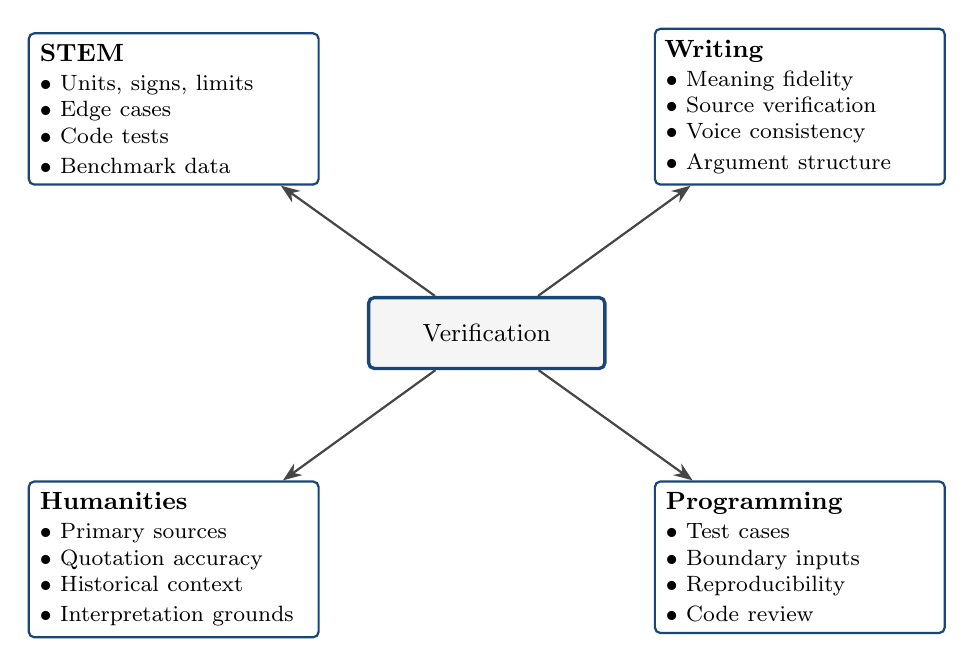
\begin{tikzpicture}[node distance=0.4cm and 0.5cm]
% Central concept node
\node[emphasis-node, minimum width=3.0cm, minimum height=0.9cm] (verify) {Verification};

% Four discipline branches
\node[framework-node, above left=1.4cm and 0.6cm of verify, minimum width=3.6cm, minimum height=1.7cm, align=left, text width=3.4cm] (stem)
  {\textbf{STEM}\\[1pt]
   \footnotesize $\bullet$ Units, signs, limits\\
   \footnotesize $\bullet$ Edge cases\\
   \footnotesize $\bullet$ Code tests\\
   \footnotesize $\bullet$ Benchmark data};

\node[framework-node, above right=1.4cm and 0.6cm of verify, minimum width=3.6cm, minimum height=1.7cm, align=left, text width=3.4cm] (writing)
  {\textbf{Writing}\\[1pt]
   \footnotesize $\bullet$ Meaning fidelity\\
   \footnotesize $\bullet$ Source verification\\
   \footnotesize $\bullet$ Voice consistency\\
   \footnotesize $\bullet$ Argument structure};

\node[framework-node, below left=1.4cm and 0.6cm of verify, minimum width=3.6cm, minimum height=1.7cm, align=left, text width=3.4cm] (humanities)
  {\textbf{Humanities}\\[1pt]
   \footnotesize $\bullet$ Primary sources\\
   \footnotesize $\bullet$ Quotation accuracy\\
   \footnotesize $\bullet$ Historical context\\
   \footnotesize $\bullet$ Interpretation grounds};

\node[framework-node, below right=1.4cm and 0.6cm of verify, minimum width=3.6cm, minimum height=1.7cm, align=left, text width=3.4cm] (programming)
  {\textbf{Programming}\\[1pt]
   \footnotesize $\bullet$ Test cases\\
   \footnotesize $\bullet$ Boundary inputs\\
   \footnotesize $\bullet$ Reproducibility\\
   \footnotesize $\bullet$ Code review};

% Connecting lines
\draw[flow-arrow] (verify) -- (stem);
\draw[flow-arrow] (verify) -- (writing);
\draw[flow-arrow] (verify) -- (humanities);
\draw[flow-arrow] (verify) -- (programming);
\end{tikzpicture}
\caption{\textbf{Verification across disciplines.} The verification habit is constant; the specific checks vary by domain. Every discipline has a small set of routine checks that catch common errors in routine tasks; these checks do not on their own certify correctness or sound judgment. Students should learn the verification toolkit appropriate to each course they take.}
\label{fig:verification-disciplines}
\end{figure}

\subsection{Verification in STEM courses}
\label{subsec:stem-verification}%
\index{verification!in STEM}

In STEM courses, verification often means testing the work against structure.

You might check units, signs, limiting cases, special cases, order of magnitude, known formulas, benchmark examples, code output, or experimental data. You might solve a simpler version of the problem. You might compare two independent derivations. You might ask whether the result behaves sensibly when an input becomes very large, very small, or zero.

For code, useful checks include small test cases, boundary cases, reproducibility, comments explaining the logic, and comparison with a known implementation.

For laboratory work, useful checks include instrument limits, measurement error, procedural consistency, data provenance, and whether the conclusion follows from the actual results.

For mathematics, statistics, and other quantitative work, a quick verification kit is:

\begin{itemize}
\item Check a trivial or special case (for example, $x=0$, $x=1$, or a known solution).
\item Check a limiting case (large or small parameter, asymptotics).
\item Check units, dimensions, and signs for each term.
\item Compare to a known formula or theorem statement.
\item Run one independent derivation or route (for example, reach the same result by a second method).
\end{itemize}

These five checks are quick first-pass screens, not proof of correctness; an independent derivation can take much longer. If a result fails one of them, the underlying work needs another look before submission.

\subsection{Verification in writing courses}
\label{subsec:writing-verification}%
\index{verification!in writing}

In writing courses, verification often means checking meaning, evidence, and voice.

After AI-assisted revision, compare the draft to your original purpose. Did the thesis change? Did the AI add a claim you did not intend? Did it make your tone too formal, too vague, or too certain? Did it remove an important nuance?

A useful practice is to write a short author's note after revision:

\studentprompt{In this revision, I changed the structure by moving the evidence earlier. I rejected the AI suggestion to make the claim stronger because the source did not support that level of certainty.}

That note helps you remain the author.

\subsection{Verification in humanities courses}
\label{subsec:humanities-verification}%
\index{verification!in the humanities}

In humanities courses, verification often means returning to the text or source.

AI can summarize, but it can also flatten ambiguity. It may miss irony, context, genre, translation issues, or the difference between a primary source and a later interpretation. If you use AI to explore a text, return to the passage itself. Ask whether the evidence supports the interpretation.

Do not let AI replace close reading.

\subsection{Verification in social science courses}
\label{subsec:social-science-verification}%
\index{verification!in the social sciences}

In social science courses, verification often means examining evidence, method, and causal claims.

Ask whether the data support the conclusion. Ask whether there are confounders. Ask whether a claim is descriptive, causal, predictive, or normative. Ask whether the sample is appropriate. Ask whether the method can answer the question being asked.

AI may help you generate alternative explanations. It cannot decide which explanation the evidence supports unless you check the evidence yourself.

\subsection{Verification in professional and applied courses}
\label{subsec:professional-verification}%
\index{verification!in professional fields}

In professional courses, verification often includes ethics, privacy, standards, and consequences.

If you are working with cases, clients, patients, designs, policies, or institutional data, ask whether AI use is permitted. Check whether the work includes sensitive information. Confirm that recommendations follow professional standards and course expectations.

A fluent answer can still be unsafe, unfair, or irresponsible.

\subsection{Verification in graduate research}
\label{subsec:graduate-research-verification}%
\index{verification!in graduate research}

Graduate research raises the verification bar. The standards of independent competence and tool-augmented practice that apply in coursework apply with extra force in research, where errors propagate through manuscripts, citations, and into the literature itself. Graduate students who use AI in their research should treat verification as part of the research workflow rather than a final check before submission. The full protocol appears in Appendix~\ref{app:sciwriting}; this subsection summarizes the core practices.

A graduate researcher should be able to defend every result, citation, computation, and interpretation in their work without reference to AI. The defense need not be unaided in real time, but the underlying understanding must be the researcher's own. If a reviewer asks ``why did you choose this approach,'' the answer should reflect scientific judgment, not tool-mediated procedure. Three workflow practices support this standard.

\textit{Independent attempt before tool use.} Begin every nontrivial research task with the researcher's own attempt: a proof outline, a model setup, a literature shortlist, a code sketch. The independent attempt is what AI assistance refines. If AI sees the problem first, the researcher's framing risks becoming AI's framing; a published paper that originated this way often shows it in subtle inconsistencies that reviewers find before authors do.

\textit{Citation discipline.} Every cited source must exist, must be read, and must support the claim being made. AI tools can produce citations that look correct but reference the wrong year, the wrong journal, or the wrong author combination, a failure mode documented empirically for AI-generated bibliographies \citep{walters2023fabrication}. Verification against MathSciNet, Web of Science, the publisher's own record, or the journal page itself is non-negotiable. Dialogue~3 in \cref{sec:dialogues-strong} illustrates exactly this kind of catch.

\textit{Audit-and-repair.} For mathematical and computational work, AI-produced derivations and code should be treated as drafts to audit, not as results to accept. The audit identifies where each step uses each hypothesis, what edge cases are excluded, and where the derivation could fail. The graduate-mathematics version of this practice is GMIP D2 (proof construction and proof repair), described in detail in Appendix~\ref{app:gmip}; analogous practices exist in computational science (input validation, boundary tests, comparison against analytical solutions) and in empirical work (sensitivity to parameter choices, robustness across specifications).

These practices are not separate from research. They are research, in an environment where AI-fluent text can pass shallow inspection. Researchers who internalize them publish more carefully, defend their work more easily under questioning, and contribute to a literature that remains trustworthy as the volume of AI-assisted scholarship grows.

\section{Disclosure}
\label{sec:disclosure}%
\index{disclosure}

Disclosure is not a confession. It is a record of process.

When an instructor permits AI use and asks for disclosure, your goal is to be factual and clear. State what tool you used, how you used it, what it contributed, what you changed, and how you verified the result. Templates you can adapt are at \texttt{students/disclosure-templates.md}.

\subsection{A short disclosure template}
\label{subsec:short-disclosure}%
\index{disclosure!templates}

Use this when AI played a small role.

\begin{quote}
\textbf{AI disclosure:} I used an approved AI tool to generate practice questions, check grammar, or suggest revision questions. I reviewed the output and made the final choices myself.
\end{quote}

\subsection{A fuller disclosure template}
\label{subsec:full-disclosure}

Use this when AI shaped the process more substantially.

\begin{quote}
\textbf{Tools used:} Name the tools used, if any.\\
\textbf{Tool role:} Describe what the tools helped with.\\
\textbf{Student role:} Describe what you wrote, revised, checked, or decided.\\
\textbf{Accepted, changed, or rejected:} Describe the AI contributions you used, revised, or set aside.\\
\textbf{Independent verification:} Describe how you checked important claims, sources, data, code, or reasoning.\\
\textbf{What I can explain without AI:} Name the main parts of the work you can now explain on your own.
\end{quote}

\subsection{What good disclosure does}
\label{subsec:good-disclosure}

Good disclosure helps your instructor see your thinking. It also protects you from two mistakes: pretending AI was not used when it was, and giving AI more credit than it deserves.

The level of disclosure should match the assignment. Minor grammar help may need only a brief note. A project that used AI for brainstorming, code, revision, and source checking needs more detail.

\subsection{Thread sharing}
\label{subsec:thread-sharing}%
\index{thread sharing}

When an instructor asks to see the AI conversation that produced your work, sharing the chat link or transcript is, as of this writing, a routine option. Most major platforms (ChatGPT, Claude, Gemini, Copilot, and others) support a share function that produces a read-only link to the conversation. The companion repository's \texttt{students/sharing-ai-conversations.md} guide describes the operational steps for each major platform.

Thread sharing is among the most informative forms of disclosure available to a student. It is a record of the interaction, not proof of authorship. A written disclosure template, however careful, depends on your account of what the AI contributed. Thread sharing lets your instructor see what was actually asked and what was actually returned. The gap between your account and the underlying interaction narrows. For an instructor's purposes, this is sometimes the difference between trusting the work and having to ask further questions.

Two honest limits deserve naming. First, thread sharing presumes the shared thread is the one that actually produced the work. A student who runs a polished AI study session for show while drafting the actual work in a separate, unshared chat has not solved the disclosure problem; they have only relocated it. The translation test in \cref{sec:compact} is the structural safeguard that narrows this gap, because the test asks what the student can do regardless of which thread produced what. Second, thread sharing must respect privacy: the considerations described in \cref{sec:privacy} apply to anything visible in a shared thread, including identifying information about classmates, instructors, or third parties. Edit or redact before sharing if any such material appears, and ask your instructor for an alternative if redaction would distort the record. The same applies to your own disclosures: if a thread contains course frustrations, learning struggles, or off-topic personal material you would rather not hand over, review and redact it, or keep gradeable work in a separate, clean thread.

\section{Privacy and data protection}
\label{sec:privacy}%
\index{privacy and data protection}

Before uploading material to an AI system, ask whether you have the right to share it. Many AI tools are run by outside companies. Some retain data. Some may use inputs to improve services. Some institutional tools may have stronger privacy protections, but you should not assume that every tool is safe for every kind of information.

Unless your instructor or institution has clearly approved the tool for that use, do not upload:

\begin{itemize}
\item private information about classmates;
\item unpublished research data without permission;
\item patient, client, or human-subject information;
\item restricted exam questions or solutions;
\item confidential institutional documents;
\item private correspondence;
\item recommendation letters or evaluations;
\item copyrighted course material if your instructor has not permitted it;
\item personal data that could identify someone else.
\end{itemize}

If you are unsure, do not upload the material. Ask your instructor how to proceed.

Privacy is not only a legal concern. It is part of academic trust. Ethical guidance for AI and data use in teaching stresses that learners and educators should handle data systems with care, transparency, and attention to risk \citep{europeancommission2022ethical}.

\chapter{In Class and Across Disciplines}
\label{ch:in-class-and-across-disciplines}%

\section{Small classes and the Oral-Defense Model}
\label{sec:small-classes}%
\index{Oral-Defense Model}\index{class size!small classes}

An \keyterm{oral defense} is a live conversation or examination in which a student explains submitted work and answers questions about it. Small classes often allow more flexible AI use because the instructor can ask students directly about their work. Examples include seminars, capstones, advanced labs, writing workshops, and many graduate courses. The defining feature is class size, not course level: a small introductory seminar uses the same Oral-Defense pattern as a small graduate seminar, even though the assignment-category mix and AI autonomy granted are likely to differ.

In these courses, you may be asked to defend AI-assisted work in conversation. That defense may look different across fields.

\begin{description}
\item[STEM.] Explain a derivation, model, computation, experiment, or code segment.
\item[Writing.] Explain your thesis, structure, evidence, and revision choices.
\item[Humanities.] Defend an interpretation by returning to the text or source.
\item[Social sciences.] Explain your method, evidence, assumptions, and limits.
\item[Professional programs.] Justify a recommendation, privacy choice, or ethical judgment.
\item[Creative work.] Explain process, iteration, constraint, and authorship.
\end{description}

The main standard is the same:

\begin{quote}
\textbf{If you submitted it, you should be able to explain it.}
\end{quote}

You can use AI to prepare for this kind of questioning. Ask it to play the role of a skeptical instructor. Ask it to question your assumptions. Ask it to find the weakest part of your explanation. Then practice answering without looking at the AI response.

\section{Large classes and the Evidence-of-Thinking Model}
\label{sec:evidence-of-thinking}
\label{sec:large-classes}%
\index{Evidence-of-Thinking Model}\index{class size!large classes}

Large classes cannot rely on one-on-one oral exams for every student. Instead, they often use scalable \keyterm{evidence of thinking}: process artifacts that show how a student reasoned, revised, verified, explained, or made choices. Most large classes are introductory or service courses simply because that is where enrollment concentrates, but the model is class-size-driven, not level-driven: a large advanced course uses the same evidence-of-thinking patterns.

You may be asked to complete short no-AI quizzes, write in class, submit a draft history, explain one step from your homework, critique a flawed AI answer, provide a process log, verify sources, record a short explanation, or participate in a random oral audit.

These practices are not meant to assume misconduct. They are meant to protect learning. In a world where AI can produce polished answers, instructors need ways to see the work behind the answer.

A common pattern is the homework-to-quiz check. You complete AI-allowed homework, then answer a short no-AI question about the same idea in class. This checks whether the homework became part of your understanding.

Another pattern is the audit-and-repair task. You receive an answer that may contain a subtle error. Your job is to find the error, explain why it matters, and repair it. This is one of the most useful AI-era skills because it rewards judgment over fluency.

The simplest pattern of all is to change what the grade rests on. Many experienced instructors already do this without calling it a strategy: they make homework a small share of the grade, often only a few percent, and place the real weight on in-person, closed-book assessment. When the grade depends on what a student can do in a proctored setting, it matters far less how they studied, because AI cannot sit the exam for them. Homework becomes practice, and AI-assisted practice is often good practice. This model verifies nothing about the homework itself, which is the point: it removes the incentive to hide AI use rather than trying to detect it. Courses with a strong in-person exam tradition may find this the least disruptive path of all, and it solves the AI-on-homework problem with almost no added labor. The trade-off is that it concentrates the assessment into a few high-stakes moments, which suits some subjects better than others and some students less well than others. Where a course can carry that trade-off, this is often the least effort for the most protection.

Many courses fall between the small-class and large-class extremes. They are too large for individual oral defenses on every assignment, but small enough for some direct contact, or arranged so that lab time supports oral defense even at medium enrollment. Part~\ref{part:instructor} (\cref{i:sec:hybrid-model}) describes the resulting Hybrid Model that combines elements of both. As a student in a hybrid course, your experience may include occasional oral conferences, often at the start of the term for calibration and again at major project milestones. Alongside them, you may keep continuous process documentation through Plan-Use-Verify artifacts on regular assignments. The expectations are the same: explain what you submitted, verify what you used, own the work.

\section{Asking better questions in mathematics and related STEM disciplines}
\label{sec:better-questions}%
\index{mathematics!asking better questions}

\Cref{subsec:ask-for-help} introduced the general principle: a useful AI question keeps the central thinking with you. The math-specific patterns from this Part and the next are consolidated in Appendix~\ref{app:math-qr} for readers who want them in one place. This section extends that principle to mathematics specifically, where AI use follows two patterns within one spiral. For computational work (calculus, numerical methods, modeling), strong prompts ask AI to check, debug, and probe rather than to solve. For proof-based work (real analysis, abstract algebra, topology), strong prompts ask AI to critique, generate examples, and identify gaps rather than to write the proof.

For computational mathematics:

Weak prompt:

\studentprompt{Solve this problem.}

Stronger prompt:

\studentprompt{Ask me one question that would help me decide which method applies.}

Weak prompt:

\studentprompt{Explain compactness.}

Stronger prompt:

\studentprompt{Give me one example, one non-example, and one common false belief about compactness.}

For proof-based mathematics, the same pattern looks like this. The strong prompts preserve the student's role as the proof-builder.

Weak prompt:

\studentprompt{Prove this theorem for me.}

Stronger prompt:

\studentprompt{Here is my proof attempt. Identify the first point where the logic may fail, but do not rewrite the proof.}

Weak prompt:

\studentprompt{Check my proof.}

Stronger prompt:

\studentprompt{Identify whether each hypothesis in the theorem is actually used in the proof. If any hypothesis is unused, ask whether the theorem can be strengthened by removing or weakening that assumption.}

These prompts train the use of AI as a mathematical coach rather than a solution engine.

The same two-mode split appears in related quantitative and computational STEM disciplines. In physics, the modes are calculation versus principle-identification: weak prompts ask AI to solve the problem; stronger prompts ask AI which principle or conservation law should apply before the algebra begins, or whether a result reduces correctly to a known limiting case. In computer science, the modes are coding versus algorithm design: weak prompts ask AI to write the code; stronger prompts ask AI to identify edge cases or to critique the proposed algorithm before any code is generated. In statistics, the modes are computation versus methodological justification: weak prompts ask AI to run the analysis; stronger prompts ask AI whether the test's assumptions are met or what would change if a key assumption were violated. The pattern holds: the stronger prompt always keeps the field-specific judgment with the student.

A deeper pattern is worth naming. Cognitive psychologists have spent decades evaluating which study techniques actually improve learning. Practice testing (quizzing yourself), distributed practice (spreading study over time), elaborative interrogation (asking why a fact is true), and self-explanation (stating in your own words how a new idea relates to what you already know) all show measurable benefit. Highlighting, rereading, and summarizing show much weaker benefit \citep{dunlosky2013improving}.

AI tools are study-technique amplifiers. Whatever technique you ask AI to support, AI will support it efficiently. Asked to summarize a reading you have not yet engaged with, AI amplifies a technique that has limited learning value. Asked to highlight what is important, AI amplifies a technique that has limited learning value. Asked to test you on material you have studied, AI amplifies a technique that has strong learning value. Asked to ask you why something is true, AI amplifies a technique that has strong learning value. The prompt determines which amplification you receive. This is why weak prompts tend to ask AI to do the low-utility work for you, while stronger prompts tend to keep the high-utility work yours.

\section{A practical study routine}
\label{sec:study-routine}%
\index{study routine}

Here is a weekly routine for using AI without weakening your learning. Worked versions of this routine, in statistics, programming, physics, and mathematics, are at \texttt{students/study-sessions/}.

Before class, skim the assigned material and write down two questions. If you use AI, ask it to explain background concepts, not to replace the reading.

After class, close your notes and write a short summary from memory. Then use AI to quiz you. Ask for one question at a time. Answer before seeing feedback.

When starting homework, attempt each problem first. If you are stuck, ask for a hint or a simpler related example. After finishing, ask AI to check for possible gaps, but verify the final answer yourself.

When writing, draft first. Then ask AI to identify unclear points, missing evidence, or possible objections. Revise in your own words.

Before an exam or oral defense, ask AI to question you. Practice explaining without looking at notes. Focus on the places where you hesitate.

A simple way to make these habits stick is to convert them into when-then plans. Some examples:

\begin{itemize}
\item When I receive AI feedback on a proof or paragraph, then I close the AI window before writing my final version.
\item When I finish AI-assisted homework, then I work one nearby problem without AI before submitting.
\item When I cannot explain a step in my own words, then I do not submit the work yet.
\end{itemize}

The when-then form turns a vague intention into a trigger-action plan and tends to improve follow-through compared to general resolutions, a pattern documented in the implementation-intentions literature \citep{gollwitzer1999implementation}.

This routine uses AI as a scaffold. It does not let AI carry the weight.

\section{Asking better questions in the humanities, social sciences, and professional fields}
\label{sec:better-questions-nonstem}%
\index{humanities}\index{social sciences}\index{professional programs}

The previous section described how AI use differs across the quantitative disciplines. The same care pays off outside them, in fields where the work is interpretation, empirical inference, or applied judgment rather than calculation or proof. The spiral does not change, but what counts as a good question and as a real verification differs by field.

\subsection{Interpretive disciplines}
\label{subsec:interpretive-disciplines}%
\index{interpretive disciplines}%
\index{humanities!interpretive work}

In literature, history, philosophy, and other interpretive fields, the work is an argument about meaning supported by evidence from texts. AI is most useful as a source of context and as a sparring partner for an interpretation you have already drafted. It is least safe when it supplies the interpretation itself. The reason is that the interpretation is the thing being assessed: a reading produced by AI tells your instructor nothing about whether you can read.

A productive pattern is to draft your own reading first, then ask AI to argue against it. Ask for the strongest objection to your thesis, for a passage that complicates it, or for the historical context a first-time reader would miss. Treat each answer as a lead to check rather than a conclusion to adopt. The characteristic verification move is return to the source: every contextual claim is checked against the assigned text or a cited document, and any detail the sources do not support is dropped. A claim about what an author intended, what a period believed, or what a term meant is only as good as the passage you can point to.

The failure mode to avoid is fluent paraphrase. AI can produce a confident, well-organized reading of almost any canonical text, and a confident reading is easy to mistake for a correct one. The discipline is to keep the argument yours and let the text, not the model's fluency, decide what the evidence will bear.

\subsection{Empirical social science}
\label{subsec:empirical-social-science}

In economics, sociology, political science, psychology, and the other empirical social sciences, the work is an inference about people or institutions drawn from data. The central difficulty is that correlation is easy to find and causation is hard to defend. AI is most useful for widening the set of explanations you consider and for stress-testing a design you have already sketched. It is least safe when it is allowed to draw the conclusion. A plausible-sounding causal story is exactly what the method is meant to discipline.

A productive pattern is to specify your question, your data, and your candidate explanation first, then ask AI what you might be missing: which confounders you have not measured, which alternative specification would change the result, which population the finding may not generalize to. Sort each suggestion into those you can test in your data and those that remain speculative. The characteristic verification move is to run the check: where a suggested confounder is measured, see whether including it moves the estimate; where it is not, record it as a limitation rather than a result. A model's confidence about an effect is not evidence; your data, your design, and the size of your sample are.

The failure mode to avoid is borrowed certainty. AI will narrate a clean causal mechanism for almost any correlation, and a clean mechanism is persuasive in a way raw association is not. The discipline is to keep the claim no stronger than the design supports, and to let the evidence, not the fluency of the story, set the limit.

\subsection{Professional and applied fields}
\label{subsec:professional-fields}

In nursing, law, business, education, and other professional programs, the work is applied judgment under real constraints, measured against authoritative standards: clinical guidelines, statutes and case law, accounting rules, professional codes. AI is most useful for framing a case, surfacing considerations, and rehearsing the reasoning you will later have to perform unaided. It is least safe when it is treated as the authority. In these fields the authority is the standard, and an answer that cannot be traced to it is not yet professional work.

A productive pattern is to reason through the case yourself first, then ask AI to challenge it: what a more cautious practitioner would do differently, which fact would change the recommendation, which guideline or rule bears on the decision. The characteristic verification move is to check against the source of authority: the current clinical guideline, the controlling statute, the applicable standard, not the model's summary of it. The summary can be outdated or wrong on exactly the detail that matters. A confident answer that conflicts with the governing standard is a hazard, not a help.

The failure mode to avoid is the confident wrong answer. AI can produce advice that reads like competent professional work while being wrong in a way only a trained eye catches, and in applied fields a wrong answer delivered confidently is the most dangerous kind. The discipline is to let the standard, and eventually your own examined judgment, decide, and to remember that the point of the training is to become the person who can tell when the confident answer is wrong.

\section{Discipline examples}
\label{sec:discipline-examples}

The verification subsections in \cref{sec:verification} listed verification techniques per discipline. This section walks through five short vignettes showing the whole Learning Spiral in action across fields: frame a question, try to solve, ask for help, work independently, verify, reflect and disclose. Each vignette is a compressed version of an honest week in a course. Your instructor's policy always comes first.

\subsection{STEM example}
\label{subsec:stem-example}

A physics student starts a problem on energy conservation. \emph{Try to solve}: she sketches a free-body diagram, writes down the conservation equations she remembers, and gets stuck on which surface friction does work. \emph{Ask}: she asks AI for one hint about how to identify the correct system boundary, not for the solution. \emph{Work}: with the hint, she completes the algebra and arrives at a numerical answer. \emph{Verify}: she checks units, tests the limiting case where friction is zero against the textbook formula, and confirms the answer's order of magnitude. \emph{Reflect and disclose}: she records that AI helped with the system-boundary identification; the rest is hers, and she can explain the steps without notes.

This is responsible use because AI helped her enter the problem without replacing the reasoning.

Within mathematics, the practical use of AI differs between proof-based courses (for example, real analysis, abstract algebra, topology) and computational courses (for example, calculus, numerical methods, modeling). Proof-based work centers on choosing the right argument and verifying that each hypothesis is used; AI is most helpful as a critic of proof attempts and a generator of examples and non-examples. Computational work centers on choosing the right method and verifying the result; AI is most helpful as a debugger of code and a checker of intermediate calculations. The two patterns share the same spiral, but the verification moves and the prompt patterns are tuned differently.

\subsection{Programming example}
\label{subsec:programming-example}%
\index{computing and programming}

A student writes a data-cleaning function. \emph{Try to solve}: he runs the code and observes that the output looks wrong on rows with missing values. \emph{Ask}: he asks AI to suggest diagnostic tests rather than rewriting the function. \emph{Work}: he builds three small test cases the AI suggested, plus one he thought of himself. \emph{Verify}: the tests reveal that missing values are passed through as zeros rather than handled separately; he revises the function and reruns the tests until they pass. \emph{Reflect and disclose}: his submission includes the tests as part of the work, with a note that AI suggested the diagnostic-test approach; the analysis of test outcomes and the fix are his.

This is responsible use because the student used AI to improve debugging, not to hide ignorance.

\subsection{Writing example}
\label{subsec:writing-example}

A student is drafting an essay on labor history. \emph{Try to solve}: she writes a full draft from her notes and the assigned readings, identifying the paragraph she's least confident about. \emph{Ask}: she asks AI to identify where the argument loses focus, without rewriting it. \emph{Work}: AI flags her third paragraph; she returns to the source she cited there and finds her evidence is thinner than her claim. \emph{Verify}: she rewrites the paragraph in her own words, narrowing the claim to what the evidence supports; she rejects an AI suggestion that would have inflated her wording back to the original level of certainty. \emph{Reflect and disclose}: her disclosure block notes that AI helped with diagnostic critique on one paragraph; the thesis, evidence, and final wording are hers.

This is responsible use because the student remains the writer and lets the evidence control the claim.

\subsection{Social science example}
\label{subsec:social-science-example}

A student is analyzing a study about education and income. \emph{Try to solve}: she works through the dataset codebook and lists the variables she thinks matter. \emph{Ask}: she asks AI to suggest possible confounders she may have missed. \emph{Work}: AI suggests six; she classifies them into those measured in the dataset and those that are speculative. \emph{Verify}: for each measured confounder, she runs a quick check on whether including it changes the coefficient of interest; for the speculative ones, she notes them as limitations. \emph{Reflect and disclose}: her writeup separates evidence-based statements from acknowledged speculation, with a disclosure block noting AI's role in confounder generation.

This is responsible use because AI helped expand the student's thinking, but the evidence controlled the conclusion.

\subsection{Professional fields example}
\label{subsec:professional-example}

A nursing student is working through a patient-care scenario. \emph{Try to solve}: she reads the case and drafts a care plan from the course material, noting the one intervention she is unsure about. \emph{Ask}: she asks AI to explain the general reasoning behind that class of intervention, not to choose the intervention for her. \emph{Work}: with the explanation, she returns to the case and tests whether her plan fits the patient's specific contraindications. \emph{Verify}: she checks AI's account against the current clinical guideline assigned in the course and corrects one detail the guideline stated differently. \emph{Reflect and disclose}: her disclosure notes that AI explained the general mechanism; the patient-specific judgment and the guideline check are hers.

This is responsible use because the clinical standard, not the model, remains the authority.

\chapter{Judgment and Limits}
\label{ch:judgment-and-limits}%

\section{When not to use AI}
\label{sec:when-not-to-use}%
\index{AI!when not to use}

Sometimes the best use of AI is not to use it.

Do not use AI when the assignment forbids it. Do not use AI when the task is designed to build fluency through practice. Do not use AI when it would expose private information. Do not use AI when you are too tired to check the result. Do not use AI when using it would make you skip the part of the work you most need to learn.

This last case is common. If you are weak at algebra, do not use AI to bypass algebra practice. If you struggle to write introductions, do not ask AI to write every introduction. If you are learning to read difficult texts, do not let AI summarize every text before you have faced it yourself.

Use AI where it strengthens your learning. Avoid it where it removes the struggle that the course is trying to teach you how to handle.

It helps to notice your own pattern. Every so often, look back over a day of coursework and sort your AI use into two kinds. In the first, you went to the tool with a purpose: a specific question, a draft to test, a step you were stuck on. In the second, you reached for it out of habit, took what it gave you, and moved on. The first is you using the tool. The second is the tool using you. You do not have to be all of one kind. But if the second is most of your day, you are learning less than you think. The fix is in your hands: before reaching for AI, ask what you are trying to do, and whether you could do it yourself.

One case deserves its own mention. Some learning comes from other people. A classmate explains it a different way. Office hours catch the thing you could not name. A study group works through the hard part together. AI is there every hour and never makes you feel slow, so it can quietly crowd these out. A good AI tutor beats no help, and sometimes beats a rushed one. But if reaching for it means you stop talking to the people around you about the work, you have given up something you will miss. Use AI to prepare for those conversations. Do not use it to avoid them.

One kind of conversation is worth seeking out on purpose. Find someone who will argue with you. A classmate who pokes holes in your reasoning, who asks why your method works and not just whether the answer matches, makes you defend your thinking out loud. An agreeable tutor rarely does that, and an AI built to be helpful does it even less. The student who learns to find the weak step in a friend's argument is the one who catches the confident mistake in a chatbot's. Practice that with people. It is how you build the judgment you need for the times the machine is the only one in the room.

If a question arises about whether work is yours, process evidence matters. AI detection tools are not perfect, and research has found that GPT detectors can misclassify non-native English writing as AI-generated \citep{liang2023gpt}. Your best protection is honest disclosure, draft history, verification notes, and the ability to explain your work.

\subsection{The choice not to use AI at all}
\label{subsec:conscientious-objector}%
\index{conscientious objector}%
\index{refusing AI}

Some students choose not to use AI for any coursework, on grounds beyond what specific assignments require. The reasons vary: environmental concerns about the energy cost of large-model inference, labor concerns about how training data was sourced and how AI is reshaping professional work, ethical concerns about complicity in harms the technology produces. From some fields, especially in the humanities, the social sciences, and the arts, the position is sometimes stated more strongly: there is no ethical use of AI in their discipline at the present moment.

This guide is not written to talk those students out of their position. The framework still applies, but the application is different. Every assignment is implicitly \NAI{} for a student who has chosen not to use AI; the Learning Spiral becomes the practice they were going to use anyway; the Student's Trilemma names the predicament they are still asked to navigate when peers are using AI freely. What the framework offers is vocabulary for the situations they will find themselves in: grading curves shaped by tools they do not use, group projects where teammates do, courses where the instructor assumes AI use without saying so. Naming the patterns helps a student who has chosen to abstain navigate a coursework environment being reshaped around them.

The institutional implications are developed in Part~\ref{part:institutional}.

\section{What to do when you are unsure}
\label{sec:unsure}

AI policies vary by course. They may even vary by assignment within the same course. If you are unsure, ask your instructor before using AI in a way that affects submitted work.

A good question is specific:

\studentprompt{For this assignment, may I use AI to generate practice questions or critique my draft if I disclose that use?}

Another useful question is:

\studentprompt{May I use AI to debug code if I include a short note explaining what I tested and what I changed?}

Avoid vague questions such as ``Can I use AI?'' That question is often too broad. Ask about the role you want AI to play.

If you already used AI and are unsure whether the use was allowed, tell your instructor early. It is usually easier to correct a misunderstanding before submission than to explain it afterward. Part~\ref{part:instructor} describes how instructors design assignments and what they look for in disclosure; reading the relevant section there can help you frame the conversation.

A related situation deserves a note.\index{disability accommodation}\index{disability accommodation!campus office} If you rely on AI as part of a documented disability accommodation, an assignment's AI-use rule and your accommodation can appear to conflict. This happens, for instance, when an assignment restricts AI but an approved assistive tool depends on it. You do not have to resolve this on your own. Raise it early with your instructor and your campus disability or accessibility office, who can confirm how the accommodation and the assignment's rules fit together. Disclosing AI use does not require revealing the accommodation behind it; that is arranged privately with the instructor and the office.

\section{Working with AI on group assignments}
\label{sec:group-assignments}%
\index{group assignments}

Group and team assignments raise a question the rest of this guide answers only for individual work: how AI use is handled when the product is shared. The word collaboration is worth pinning down first. Collaboration here means working with your classmates, not the AI-as-collaborator role of the \AIC{} category. A group project can use AI under any of the four categories, and the team needs to know which one applies before it starts.

The standards you already know apply at the level of the group. Agree early on how AI may be used, and on which parts of the work, so that no member is surprised later. Keep your own verification notes for the portions you contribute, and be ready to explain them, because the translation test in \cref{sec:compact} does not stop applying when the work is shared. When the assignment asks for disclosure, the group discloses together: what the team used AI for, what each member verified, and what the group changed or set aside. A single joint disclosure is usually clearer than separate notes that do not line up.

When group work ends in a presentation, the room reads the result; it cannot read what your group did to get there. Lead with the moment the tool handed you something plausible you did not accept, and show what made you stop. Put the output beside what you changed. A group that checked nothing has nothing to show. This is the compact performed aloud: work you can explain, verification you can show, and responsibility you take in front of people who can ask.

The quieter risk in group work is the one this guide has warned about throughout, sharpened by the division of labor. It is easy to let a teammate, or the AI, take the part you most need to learn, and to finish the project having practiced only what you were already good at. Treat your share of a group assignment the way you would treat your own work: try the hard part first, and use AI for help rather than replacement. Make sure that when the project is done you can explain more than your own slice of it. How instructors design and grade group work under these conditions is described in \cref{i:sec:group-assignments}.

\section{Evidence base and limits of the guide}
\label{sec:evidence-limits}%
\index{evidence base and limits}

This guide draws on three kinds of evidence: learning science, emerging research on AI-supported tutoring, and institutional guidance on responsible AI use. The learning-science foundation is mature enough to support several strong claims. Active retrieval, spaced practice, self-explanation, and elaborative interrogation help students learn because they require the learner to do cognitive work \citep{dunlosky2013improving}.

Research on computer-assisted learning did not begin with generative tools. Intelligent tutoring systems and educational software have been studied for decades, and what changed is not that the questions are new but that a general-purpose tool reached every student at once, outside any course design.

The AI-specific evidence is newer and still heterogeneous, but a clear pattern is emerging: AI helps most when it is embedded in active learning, verification, feedback, and independent reconstruction. Across methodologies and disciplines, the results so far point the same way: the design of AI use determines whether learning improves, stays flat, or declines. \index{Bastani field experiment|textbf}A pre-registered randomized trial by Bastani and colleagues gave nearly a thousand high-school mathematics students one of two tools. An unrestricted ChatGPT-style interface raised practice performance by 48\% but cut exam performance by 17\% against no-AI controls. A guardrailed AI tutor raised practice performance by 127\% with no exam-performance loss \citep{bastani2025generative}. \index{Kestin AI-tutor study|textbf}A randomized controlled trial by Kestin and colleagues in an introductory physics course at Harvard found that a carefully designed AI tutor produced learning gains over double those of in-class active learning. The tutor was engineered around seven pedagogical practices: active engagement, cognitive-load management, growth mindset, scaffolding, feedback accuracy, timely targeted feedback, and self-pacing. The system prompt handled the first three; the platform's structured walkthrough handled scaffolding; accuracy came from the worked solutions the designers loaded in advance. Only the last two, timely targeted feedback and self-pacing, come from the medium itself \citep{kestin2025ai}. Recent meta-analyses find a positive overall effect on academic achievement \citep{sun2024does} and on higher-order thinking, strongest for problem solving and weakest for creativity \citep{zhao2025does}. Those averages and the Bastani result are not in conflict. An average pools designs that guard the student's own thinking with designs that replace it. The pooled number hides the difference that matters. That is the finding: not that AI helps or hurts, but that the design decides which. UNESCO frames AI literacy as a shared responsibility for students and teachers, not only a student skill \citep{miao2024aia,miao2024aib}; the OECD's 2026 Digital Education Outlook synthesizes the same conclusion at the international policy level \citep{oecd2026digital}.

\index{Shen and Tamkin skill-formation study}A 2026 randomized study by Shen and Tamkin points the same way from outside the classroom. Developers learning an unfamiliar programming library with AI assistance scored lower on conceptual understanding, code reading, and debugging than those who worked without it, and they did not finish meaningfully faster. The same study sorted how participants actually used the assistant and found patterns that preserved learning, each of them keeping the person engaged with the code rather than delegating it \citep{shen2026skill}. These were working developers rather than students, so the result converges with the classroom evidence rather than repeating it.

How unrestricted AI weakens learning is not settled, but several candidate mechanisms recur. Researchers describe them with overlapping names: cognitive offloading (skipping the diagnostic and evaluative steps of help-seeking), metacognitive laziness (reduced self-monitoring during AI-assisted tasks), and the crutch pattern (asking AI for solutions rather than for help). Neuroimaging evidence suggests reduced neural connectivity when students start with AI rather than with their own attempt \citep{kosmyna2025brain}. The Bastani study adds a metacognitive finding that matters here: students often do not perceive that their learning has been reduced, even when objective assessment shows it has. \index{Liu persistence trial}A 2026 series of randomized trials by Liu and colleagues points to a further mechanism. After only brief AI use, people not only performed worse once the tool was removed but also gave up sooner, which suggests that ready answers can erode persistence itself, the willingness to work through difficulty that learning depends on \citep{liu2026ai}. That study is currently circulating as a preprint, and its estimates should be read with that status in mind. The guide's emphasis on trying first, verifying, reflecting, and explaining is designed to address each of these mechanisms in turn.

For that reason, this guide avoids a simple pro-AI or anti-AI position. It treats AI as useful when it keeps you active and risky when it lets you skip the work the course is meant to teach. The best test is practical: after using AI, can you explain more, verify more, and do more on your own than you could before?

\section{A final word}
\label{sec:final-word}%
\index{Wendy}

AI can make schoolwork faster. That is not always good. Some parts of learning are slow because they require attention, memory, judgment, and practice. The goal is not to avoid all difficulty. The goal is to use help wisely.

A student who uses AI well does not hide behind it. They use it to ask better questions, test their thinking, find weak places, and improve their work. They know what the tool contributed. They know what they checked. They know what they still do not understand.

That is the standard this guide asks you to meet.

It is also the standard the author tried to meet in writing this book; the Preface describes how AI was used here, and where it was resisted.

Wendy, from the opening pages, read her incentives correctly; this guide's answer is that all three corners can be held, and these practices are how.

Use AI when it helps you think. Stop when it starts thinking for you.

\clearpage
\section{Student checklist}
\label{sec:student-checklist}%
\index{checklist, student}

Use this checklist before submitting AI-assisted work. A copy you can print or keep on a phone is at \texttt{students/checklist.md}.

\begin{itemize}[label=$\square$]
\item I know the AI policy for this assignment.
\item I made my own first attempt before using AI for substantial help.
\item I used AI for support, not replacement.
\item I checked important claims, sources, calculations, or interpretations.
\item I removed any AI-generated material I could not explain.
\item I protected private, restricted, and confidential information.
\item I disclosed AI use if the assignment required it.
\item I can explain the final work in my own words.
\item I can close AI and my notes and redo the key argument, calculation, proof, or paragraph from a blank page.
\item I know what I learned from the process.
\end{itemize}

The blank-page item is the strongest single calibration check on the list. Explanation while looking at finished work is easy to confuse with understanding; reconstruction from a blank page is harder to fake.

\section{Reference materials}
\label{sec:part1-refs}%
\index{companion repository}

The following templates are intended for student use during AI-assisted assignments. Instructors may adopt or adapt them. For institution-wide reference materials, see Part~\ref{part:institutional}.

\subsection{Template: AI account configuration}
\label{app:ai-config}

Use this six-category template to set persistent preferences in your AI platform (sometimes called custom instructions, system prompts, or memory). Copy them, adapt the bracketed parts to your situation, and paste the whole thing into your platform's preferences panel. The motivation for configuring your account at all is given in \cref{sec:setup}; the categories below are the operational template.

\begin{enumerate}
\item \textbf{Who you are and what you are studying.}

\begin{quote}
\textit{I am a [year] [undergraduate/graduate] student in [department] at [university]. I am currently taking [course names this semester]. My academic background includes [prior coursework relevant to current work]. I am using AI to support my learning, not to substitute for it.}
\end{quote}

This single paragraph gives the AI enough context to calibrate explanations to your level and your courses. Update it each semester as your courses change.

\item \textbf{How you want explanations pitched.}

\begin{quote}
\textit{Explain reasoning step by step. When I ask you to solve a problem, walk me through the approach before giving the answer; do not just give me the final answer when I am working through something I should be learning. If a concept builds on prerequisites I have not told you about, ask me what I already know rather than assuming.}
\end{quote}

The last sentence is the most important. It teaches the AI to ask, which prevents the two most common failure modes: explanations pitched too high (where you cannot follow the reasoning) and explanations pitched too low (where the AI assumes ignorance you do not have). Both waste your time.

\item \textbf{How you want uncertainty handled.}

\begin{quote}
\textit{When you are uncertain about a fact, say so explicitly. Do not invent citations, sources, or specific numbers if you do not know them. If a question is at the edge of your knowledge, tell me, so I can verify in textbooks or other sources rather than trusting an answer that might be wrong.}
\end{quote}

AI systems can produce confident-sounding wrong answers, especially for specific facts (dates, citations, equations from particular papers, statistics). Asking the AI to flag its own uncertainty may help, but it does not remove the need to verify important claims yourself.

\item \textbf{Writing style preferences.}

\begin{quote}
\textit{I write in [American English / British English / English as a second language]. [If English is not your first language: please flag passages where my phrasing might read as unclear or non-idiomatic, and suggest alternatives.] I prefer prose that is [clear and direct / formal / conversational].}
\end{quote}

The English-as-a-second-language clause matters more than it may seem. Detector tools used by some journals and some courses systematically misread non-native-English writing as AI-generated, an issue covered in Part~\ref{part:institutional} and Appendix~\ref{app:sciwriting}. If English is not your first language, telling the AI so, and asking it to help with idiomatic clarity, both improves the writing and gives you a record of what you wrote and what the AI suggested, which protects you if your work is questioned.

\item \textbf{Scope of use and integrity boundary.}

\begin{quote}
\textit{I will use AI for [studying, brainstorming, debugging, getting unstuck, checking my own work]. I will not use AI to [write assignments I am supposed to do myself, generate code I do not understand, produce text I will submit as my own work without disclosure]. When my course or assignment policy says no AI, I will not use AI for that work, regardless of what is in this configuration.}
\end{quote}

This is partly a reminder to yourself. The configuration does not override your course's rules; the assignment categories described in \cref{sec:assignment-categories} explain when AI is permitted, encouraged, restricted, or forbidden, and the assignment-level rules always take precedence over your account-level configuration. Putting the boundary in writing where you see it every time you open an AI conversation helps keep the lines clear.

\item \textbf{Optional: technical-work accuracy guard.}

\begin{quote}
\textit{For mathematical, scientific, or technical answers: show your work. For any claim that rests on a specific fact, citation, or number, flag it as one I should verify and name the source or calculation I can check it against. If I ask for code, explain what each non-obvious line does.}
\end{quote}

This is optional because it adds complexity to every answer. For students in mathematics, the sciences, and engineering, it is the single most useful addition you can make. The labels train you to read AI output critically by making the AI's confidence level visible, and the show-your-work instruction makes the verification practices in \cref{sec:learning-spiral} easier because the work is already laid out.
\end{enumerate}

\textbf{A living document.} The starter template above captures the categories that experienced academic users have found matter most. As you use AI more, you will discover specific failure modes in your own work and want to add specific instructions to prevent them. This is normal and expected. Treat your AI preferences as a living document. Periodically review what is there, prune what no longer applies, and add what you have learned the hard way to specify. After two or three semesters of use, you will have a personalized configuration that reflects your work style and your discipline's particular demands. The point of starting with the elements above is to give you the structure those experienced users converge on, so you can grow your own configuration on a sound foundation rather than discovering each lesson by repeated failure.

\textbf{Where to learn the platform-specific details.} The instructions for setting persistent preferences vary by AI platform, and the user interfaces change often enough that any specific click-by-click guide written today will be partly outdated within a year. For current instructions, consult the documentation page for whichever platform you use; major platforms (ChatGPT, Claude, Gemini, Copilot, and others) all maintain documentation on system prompts, custom instructions, or memory configuration. If your university's library, IT services, or teaching center has a guide for academic AI use at your institution, start there (see \cref{u:subsec:support}). Institutional guides usually take account of any university-licensed AI tools and the specific privacy considerations for student use.

\subsection{Template: AI use log}
\label{app:ai-use-log}

Use this template for assignments that require process documentation.

\begin{longtable}{p{0.25\textwidth}p{0.68\textwidth}}
\toprule
\textbf{Question} & \textbf{Your response} \\
\midrule
Assignment & \\
AI tool used & \\
Date used & \\
Purpose of use & \\
Prompt or question asked & \\
Useful output received & \\
Output rejected or changed & \\
Verification method & \\
What I learned & \\
What I can explain without AI & \\
\bottomrule
\end{longtable}

\clearpage
\subsection{Template: verification checklist}
\label{app:verification-checklist}

\begin{itemize}[label=$\square$]
\item I can restate the task in my own words.
\item I know which parts of the work were helped by AI.
\item I checked each major claim against an appropriate source or method.
\item I verified all quotations and citations.
\item I checked calculations, code, or data where relevant.
\item I looked for hidden assumptions.
\item I removed or rewrote anything I could not explain.
\item I can answer questions about the final work.
\end{itemize}

\subsection{Template: prompt library for learning}
\label{app:prompt-library}

\subsection*{For understanding}

\studentprompt{Explain this idea in three levels: simple intuition, course-level explanation, and one technical detail I should not miss.}

\studentprompt{Give me an example, a non-example, and a borderline case.}

\studentprompt{Ask me questions that reveal whether I understand this concept.}

\subsection*{For problem solving}

\studentprompt{Give me one hint about the main obstacle. Do not solve the problem.}

\studentprompt{What assumptions should I check before choosing a method?}

\studentprompt{What is a simpler related problem I could solve first?}

\subsection*{For writing}

\studentprompt{Here is my draft. Identify the paragraph where the argument is least clear. Do not rewrite it. Ask me revision questions.}

\studentprompt{What claim in this paragraph needs stronger evidence?}

\studentprompt{Does this revision change the level of certainty in my original claim?}

\subsection*{For coding and computation}

\studentprompt{Suggest simple test cases for this code. Do not rewrite the function yet.}

\studentprompt{What edge cases might break this algorithm?}

\studentprompt{Explain what this error message means and ask me what I have already checked.}

\subsection*{For exam preparation}

\studentprompt{Quiz me one question at a time. Wait for my answer before giving feedback.}

\studentprompt{Ask me to explain the main concept without using jargon.}

\studentprompt{Give me a flawed answer and ask me to find the mistake.}

\subsection{Template: one-page student compact}
\label{app:compact}

\begin{quote}
I understand that AI may be allowed in some parts of this course and not allowed in others. I will follow the policy for each assignment. When AI use is allowed, I will use it to support learning rather than replace my own work. I will verify important AI-assisted content, protect private information, disclose AI use when required, and submit only work that I can explain as my own.
\end{quote}

\subsection{Short glossary}
\label{app:glossary}%
\index{glossary!Part I}

\begin{description}
\item[AI-assisted Practice.] What students can do when they use AI responsibly as a permitted tool for learning, revision, analysis, coding, feedback, or exploration, without losing control of the work. The middle component of the CAT framework: asking useful questions, judging responses, comparing explanations, finding weak points, generating practice problems, revising carefully, testing code, checking assumptions, and using feedback without becoming dependent on it.
\item[AI-assisted work.] Work shaped in some way by an AI tool, including brainstorming, drafting, revision, coding, explanation, summarization, critique, or feedback.
\item[Assignment categories.] Four labels for AI use in coursework: \NAI{} (No AI), \AIT{} (AI as Tutor, study only), \AIC{} (AI as Collaborator on submitted work, with verification and disclosure), \AIS{} (AI as Object of Study). Three sit on a traffic light (\NAI{} red, \AIT{} yellow, \AIC{} green); \AIS{} is blue, off the traffic light, because the question is different.
\item[Calibration error.] The gap between what a student thinks they know and what they can actually demonstrate. AI use widens this gap if it allows recognition to substitute for production.
\item[CAT framework.] Three dimensions of student capability under AI: Core Competence (what you can do without AI), AI-assisted Practice (skill at using AI well), Trustworthiness (verification, disclosure, ownership).
\item[Core Competence.] What students must understand and be able to do without AI or with tightly bounded assistance. The first component of the CAT framework.
\item[Desirable difficulties.] Conditions that slow initial performance (productive struggle, retrieval failure, effortful reconstruction) but produce more durable learning.
\item[Disclosure.] A clear statement of how AI was used in producing an assignment.
\item[Distributed practice.] Studying material at intervals, with forgetting and re-retrieval between sessions, rather than in a single block. Also called spacing.
\item[Evidence of thinking.] Process artifacts that show how a student reasoned, revised, verified, explained, or made choices.
\item[Friction-wall failure.] The failure pattern produced when a student reaches for AI before making a real attempt at the problem. They recognize the AI's solution but cannot generate the analogous one on their own, and often cannot tell the difference. Named for the moment of productive difficulty that AI use can short-circuit.
\item[Generated citation.] A source suggested by AI. Generated citations must be checked before use.
\item[Generation effect.] The finding that information you produce is remembered better than information you only read.
\item[Honest risk.] One of the three failure modes of the Student's Trilemma: the student is honest and genuinely understands, but the grade suffers; both commitments are kept at a personal cost the incentives should not require.
\item[Illusion of competence.] The mistaken sense that you understand material you have only seen explained, including the recognition--production gap, the mastery illusion on transfer, the effort illusion, and the authorship illusion (see \cref{subsec:illusion}).
\item[Interleaving.] Mixed practice across problem types or topics, rather than blocked practice on one type at a time. Builds the discrimination skills that single-method practice does not.
\item[Learning Spiral.] The core habit this guide recommends. A question sits at the center, and five steps pursue it: try to solve, ask for help, work independently, verify, reflect and disclose. Trying and asking alternate until the idea holds. Run on every AI-assisted task. A question is not finished when you answer it. Pursued well, each finished answer opens the next question.
\item[Mentor prompt.] A standing prompt, set up before any tutoring begins, that has the AI calibrate to the student's level and goals, keep the student doing the thinking, and check in periodically rather than continuously (\cref{subsec:mentor-prompt}).
\item[Oral defense.] A live conversation or examination in which a student explains submitted work and answers questions about it.
\item[Polished hollow.] One of the three failure modes of the Student's Trilemma: the student earns the grade and discloses AI use honestly but cannot reproduce the work; the surface is right and the disclosure is clean, but the underlying competence has not formed.
\item[Practice testing.] Trying to recall information, produce a solution, or reconstruct an argument, rather than re-reading or re-watching. Also called retrieval practice.
\item[Strategic compliance.] One of the three failure modes of the Student's Trilemma: the student earns the grade and genuinely understands but hedges on how AI helped; the learning happened but the account of it is shaped to protect the grade.
\item[Student's Trilemma.] A three-way pull (like a dilemma but with one more horn) among earning the grade, being honest about how the work happened, and demonstrating genuine understanding. Each pair pulls against the third. AI sharpens each edge but did not create the trilemma. Three named failure modes are the polished hollow, strategic compliance, and honest risk.
\item[Translation test.] A diagnostic for whether a student owns their work: can they re-present it in a different form, different notation, different variables, different example, or a different representational mode (visual, mathematical, plain language)? If they can translate fluently, the work is theirs. If not, they have recognition, not production.
\item[Trustworthiness.] How well students verify, disclose, critique, and take ownership of AI-assisted work. The third component of the CAT framework. A student demonstrates trustworthiness by checking what AI produced, telling readers honestly what AI did, and standing behind the result.
\item[Try to solve.] The first step of the Learning Spiral: make an honest attempt before asking AI for help.
\item[Verification.] The act of checking AI-assisted content against reliable evidence, sources, data, tests, methods, or reasoning. The act that drives Trustworthiness in the CAT framework.
\end{description}

% ============================================================================
% PART II - INSTRUCTOR GUIDE
% ============================================================================

\part{Teaching and Assessing with AI: An Instructor Guide}
\markboth{Part~II~\textperiodcentered~An Instructor Guide}{}
\label{part:instructor}

\bookepigraph{The question is not whether a student used AI.\\It is what the work still shows.}

\textit{Part II of this book is the Instructor Guide. It helps faculty, lecturers, teaching assistants, and course coordinators design courses that remain intellectually honest, fair, and useful when students have access to powerful AI tools. It is general in scope, with especially detailed examples for STEM and research-intensive courses.}

\textit{The central premise is simple. AI-assisted education must assess two things separately: what students can do independently, and what students can do responsibly with AI. A course that ignores AI may lose assessment validity. A course that accepts AI output without safeguards may lose learning. The goal is a better middle path: teach students to use AI as a tool while preserving the habits of attention, judgment, verification, and explanation that higher education is meant to build.}

\textit{Part II is five chapters. Chapter 7 sets out the competing pressures an instructor is under. Chapter 8 covers the framework and how to design an assignment around it. Chapter 9 sets out three assessment models and when each one fits. Chapter 10 covers integrity without detectors, equity, and keeping grading consistent across a teaching team. Chapter 11 covers what it takes to run this in a real course and where the approach reaches its limits. It also carries the reference materials the earlier chapters point to. A reader who needs one thing can go to that chapter directly.}

\chapter{Orientation and the Trilemma}
\label{i:ch:orientation-and-the-trilemma}%

\section{Purpose and scope}
\label{i:sec:purpose}

Generative AI has changed the practical conditions of teaching. Students can now obtain fluent explanations, polished essays, working code, plausible citations, study questions, summaries, translations, and step-by-step solutions in seconds. These tools can help students learn. They can also make it difficult to know what a submitted artifact reveals about the student's understanding.

This guide offers a practical framework for that problem, consistent with broader guidance that treats generative AI as a tool requiring human oversight, transparency, and institutional judgment \citep{miao2023guidance}. It does not ask instructors to choose between banning AI everywhere and allowing it everywhere. Both responses are too blunt for the range of courses taught at a university. A writing seminar, a chemistry lab, a design studio, a calculus course, a history survey, and a graduate methods course need different rules. Still, they share the same underlying responsibility: preserve meaningful learning while teaching students to use modern tools responsibly.

Guides to teaching with AI exist; this one differs in sharing its framework and vocabulary with the student guide in Part~\ref{part:student} and the institutional guide in Part~\ref{part:institutional}, so the categories on your syllabus are the ones your students study and your institution can write into policy.

One point about Part~\ref{part:student} deserves saying plainly. Most students will not go looking for it. AI tools are free and take no effort to start using, and ease crowds out intention. A student who has never been asked to think about how to use AI well has no reason to seek out a guide on the subject.

The student guide reaches students when an instructor puts it in front of them. That makes you its only reliable route. Assign it, or assign the parts that match your course, and tie the reading to the first assignment where AI is permitted. A student who has read it will know what your syllabus category means, what verification looks like, and what to disclose. A student who has not will guess.

The companion repository makes the assignment concrete. Assign \texttt{students/start-here.md} in week one; it takes a student ten minutes. Have students set up the Study Partner Protocol at \texttt{companion/spp/} before the first assignment where AI is permitted. Require the checklist at \texttt{students/checklist.md} before they submit that assignment. The one-page schedule at \texttt{instructors/what-to-assign.md} lays out the full sequence and what each piece costs a student in minutes. If this is your first term teaching with AI, \texttt{instructors/first-time-guide.md} walks through the decisions in order.

The guide has four aims.

\begin{enumerate}
\item Help instructors state clear AI policies for each assignment.
\item Help instructors design assessments that reveal student thinking.
\item Help instructors teach verification, disclosure, and responsible judgment.
\item Help departments develop consistent practices across small, medium, and large courses.
\end{enumerate}

One variable runs through the rest of this Part more than any other: class size. A thirty-student seminar, a seventy-student lecture, and a three-hundred-student introductory course are completely different worlds for AI-era assessment design. Approaches that work in the seminar do not scale to the introductory course; approaches that scale may not preserve what makes the seminar valuable. The framework developed here is built around three assessment models (Oral-Defense, Evidence-of-Thinking, and Hybrid) each calibrated to a different range of class sizes, and around three design axes that include class size as the first (\cref{i:sec:three-axes}). The class-size axis recurs throughout the Part wherever the framework's recommendations bend with it. Readers whose class size is their dominant constraint may want to scan \cref{i:sec:three-axes} and the three assessment models early.

The recommendations are intentionally modest. The evidence on generative AI in education is developing quickly, and specific tools will change. Recent studies suggest that AI tutoring can support learning when designed around sound pedagogy, while unguarded access can weaken later independent performance \citep{bastani2025generative,kestin2025ai}. The durable principles are less likely to change: students need core competence, active practice, verification habits, transparent process, and fair assessment \citep{oecd2026digital,dunlosky2013improving}.

\section{Instructor outcomes}
\label{i:sec:instructor-outcomes}%
\index{learning outcomes!instructor}

After using this guide, an instructor should be able to design a course that states AI expectations clearly and assesses student learning fairly. In practice, this means being able to do the following.

\begin{enumerate}
  \item Identify the Core Competence that students must demonstrate without AI or with tightly bounded assistance.
  \item Design AI-assisted assignments that develop AI-assisted Practice rather than reward outsourcing.
  \item Assess Trustworthiness through verification, disclosure, process evidence, and explanation.
  \item Choose an Oral-Defense, Evidence-of-Thinking, or Hybrid model that matches class size and staffing.
  \item Use AI to support teaching without delegating grades, integrity decisions, or student evaluation to an automated system.
\end{enumerate}

These outcomes keep the guide focused on course design. They also make clear that AI policy is not separate from pedagogy. It is now part of pedagogy. You are not there to fill a bucket; you are there to build judgment that outlasts any tool.

\subsection{Relation to international AI competency frameworks for teachers}
\label{i:subsec:instructor-unesco}

The instructor outcomes above are scoped to course design and assessment. They sit inside the broader AI competency framework for teachers articulated by UNESCO \citep{miao2024aib}, which specifies fifteen competency blocks across five aspects (Human-centred mindset, Ethics of AI, AI foundations and applications, AI pedagogy, AI for professional development) and three progression levels (Acquire, Deepen, Create). Two aspects of UNESCO's teacher framework are particularly relevant to the instructor outcomes in this Part: \emph{AI pedagogy} (using AI to facilitate learning) and \emph{AI for professional development} (using AI to support the instructor's own professional growth). The first is the central focus of this Part; the second is addressed briefly in the discussion of faculty use later in the chapter.

\Cref{tab:instructor-unesco} sketches the correspondence. The mapping is partial because the instructor outcomes in this guide focus on how to design assignments and assess learning when AI tools are available. UNESCO's framework also covers a teacher's broader AI literacy and ethical engagement with AI in society. A faculty development program that prepares instructors for the outcomes of this Part will move them through UNESCO's \emph{Acquire} and \emph{Deepen} levels in the AI pedagogy aspect. Programs aiming for the \emph{Create} level will need to extend beyond this guide.

\begin{table}[ht]
\centering
\caption{\textbf{Instructor outcomes and the UNESCO teacher framework.} What this Part asks of an instructor is close to what the international standard asks \citep{miao2024aib}. The correspondence is partial by design. UNESCO covers AI literacy, ethical engagement, and professional development across a teaching career. This Part stays with the decisions an instructor makes about a single course.}
\label{tab:instructor-unesco}
\begin{tabularx}{\textwidth}{>{\raggedright\arraybackslash}X >{\raggedright\arraybackslash}X}
\toprule
\textbf{Instructor outcome (this Part)} & \textbf{Closest UNESCO competency block} \\
\midrule
Identify Core Competence to be demonstrated without AI & AI pedagogy: AI-pedagogy integration (\emph{Deepen}); design assignments that target core skill domains. \\
\addlinespace
Design AI-assisted assignments that develop AI-assisted Practice & AI pedagogy: AI-pedagogy integration and AI-enhanced pedagogical transformation (\emph{Deepen} and \emph{Create}). \\
\addlinespace
Assess Trustworthiness through verification, disclosure, process evidence & Ethics of AI: Safe and responsible use (\emph{Deepen}); Human-centred mindset: Human accountability (\emph{Deepen}). \\
\addlinespace
Choose an assessment model matched to class size and staffing & AI pedagogy: AI-assisted teaching (\emph{Acquire}) and AI-pedagogy integration (\emph{Deepen}). \\
\addlinespace
Use AI to support teaching without delegating grades or integrity decisions & AI pedagogy: AI-assisted teaching (\emph{Acquire}); AI for professional development: AI enabling lifelong professional learning (\emph{Acquire}). \\
\bottomrule
\end{tabularx}
\end{table}

A program that already aligns its faculty development with UNESCO's framework can adopt the instructor outcomes here as the assessment-focused operationalization of UNESCO's \emph{Acquire} and \emph{Deepen} levels in the AI pedagogy aspect, without abandoning the broader UNESCO structure.

\section{The instructor-side calibration problem}
\label{i:sec:central-problem}%
\index{calibration problem, instructor-side}\index{office hours!as an early-warning signal}\index{office hours!decline in attendance}

The same diagnostic I once used to catch a copied proof, by its notation, is what helps a teacher distinguish owned understanding from polished output today. The technology is different. The work of telling them apart is not.

A teacher with seventeen years of teaching experience told the \emph{Chronicle of Higher Education} that the work of distinguishing student writing from AI-assisted writing now consumes time that previously went elsewhere. ``I'm grading fake papers instead of playing with my own kids,'' he said.\footnote{Quoted in \citet{mcmurtrie2024professors}.} The line is one teacher's, but the predicament is widely shared. The labor cost of the calibration problem is real, and acknowledging it is the place to start.

Students sense the calibration problem from an unexpected angle. Focus groups with ninety-five undergraduates at the University of Pittsburgh in 2025 surfaced a quiet finding: some students prefer AI chatbots to faculty office hours because, as one student put it, ``with ChatGPT you can ask as many questions as you want and it's not going to judge you.''\footnote{Reported in \citet{silva2025university}.} The line is not a verdict on any particular instructor. It is a description of how the instructor's classroom now looks from the other side of the desk. A patient, infinite, non-judgmental tutor has appeared, and it is competing for the role that the instructor used to hold uncontested. It also takes something harder to replace. Office hours were an early warning. A student in trouble would show up with a question weeks before the exam, in time for the instructor to act. When that question goes to a chatbot instead, the warning does not move; it vanishes, and the first clear sign of trouble becomes the exam, too late to help. The signal was always partial, since the students who needed it most were often the least likely to come. The remedy is to build it into the course rather than wait for the office to fill: the process artifacts and in-class checks in this Part are early signals that do not depend on who shows up.

The translation test introduced for students in Part~\ref{part:student} (\cref{sec:compact}) is the same diagnostic the instructor can use. A student who cannot translate their work into different notation, with different variable names, by a different example, has produced an artifact whose origin is uncertain regardless of its surface polish. \Cref{i:sec:integrity} develops the test as a teaching tool.

When students submit AI-assisted work, instructors face a parallel problem to the one Part~\ref{part:student} named for students. The cues that previously signaled mastery, including clean prose, organized argument, articulate explanation, and polished proofs, no longer reliably distinguish students who understand the material from students who used AI to produce work that resembles understanding. A student can submit a coherent essay, a well-organized lab report, or a correctly proved theorem without having done the cognitive work that produces those things in a pre-AI environment. AI did not make the problem harder to solve; it made the problem harder to see.

This is a calibration problem for the instructor: the difficulty of distinguishing what a finished artifact reveals about \emph{this student}, separate from what AI may have contributed. The three assessment models presented later in this Part (Oral-Defense, Evidence-of-Thinking, and Hybrid) are designed to address it. They restore the signal that AI has weakened.

Reading the rest of Part~\ref{part:instructor} as a calibration-restoring project may be useful. The NAI, AIT, AIC, and AIS assignment categories are not just AI-permission categories. They are calibration choices about which dimensions of student competence each assignment measures. The verification rubrics ask students to demonstrate the gap-closing practices from Part~\ref{part:student}. The process-evidence guidance is designed to recover what the polished final product no longer reveals on its own.

Before generative AI, a submitted paper, proof, program, lab report, or problem set was never perfect evidence of learning. Students could receive help from friends, tutors, solution manuals, prior students, websites, and commercial services. AI did not create the problem of attribution. It changed the scale, speed, and polish of outside assistance.

The core assessment question is now sharper:

\begin{quote}
\textbf{What does this submitted work show that the student can understand, explain, verify, and do?}
\end{quote}

If an assignment can be completed well by a generic AI tool, the assignment may still have value as practice, but it is weak evidence of independent competence. This does not mean the assignment should be abandoned. It means the instructor should decide what the assignment is for. Is it meant to measure unaided knowledge? Is it meant to teach responsible use of tools? Is it meant to produce a polished final artifact? Is it meant to reveal process?

Recent learning-analytics research helps name the mechanisms by which a polished AI-assisted artifact can hide reduced learning. \citet{fan2025beware} describe \keyterm{metacognitive laziness}: students using generative AI on revision tasks performed measurably fewer self-monitoring activities, especially evaluation and orientation, even when their final artifact scored well. \citet{chen2025unpacking} describe a related pattern they call cognitive offloading: in their comparative analysis of student help-seeking with human experts versus AI chatbots, students working with the chatbot tended to skip the diagnostic, evaluative, and iterative stages that ordinary help-seeking includes, jumping directly from request to implementation. Both mechanisms point the same way. The artifact improves; the learning does not follow. In Fan's trial the AI group's essay scores rose while their knowledge gain and transfer showed no significant advantage. Designing assignments that make those skipped stages visible is the practical response to both mechanisms, and is the orientation behind the Plan-Use-Verify and Oral-Defense patterns in this Part.

Confusion arises when a course treats one kind of task as if it measured all of these things. In the AI era, instructors should separate them.

\section{The Instructor's Trilemma}
\label{i:sec:trilemma}%

The calibration problem in the previous section names what instructors \emph{observe}. This section names what instructors \emph{face} when they sit down to design a course, grade a stack of papers, or decide whether to raise a quiet conversation with a student about suspected AI use. Like students and institutions, instructors under AI pressure navigate a structural predicament that has not been clearly named in the discourse. Call it the \keyterm[Trilemma!Instructor's]{Instructor's Trilemma}, and it has the same three-cornered shape as the Student's Trilemma developed in Part~\ref{part:student} and the Institution's Trilemma developed in Part~\ref{part:institutional}.

Before naming the three corners, a quieter question runs underneath all of them and deserves acknowledgment. Faculty are encountering AI not only as a pedagogical challenge but as a vocational one: \emph{what am I uniquely for, in a classroom where AI can also explain, also tutor, also assess, also produce convincing prose?} The question is rarely asked aloud, partly because it is hard to ask, and partly because no answer is fully reassuring. It runs through the faculty discourse in a hundred quiet ways: the early retirement that was not planned, the senior colleague whose enthusiasm has gone flat, the conference panels titled ``the future of higher education.'' The Instructor's Trilemma does not answer this question, but it names the three forces an instructor must navigate while the question hangs in the air.

The corners are:

\begin{description}
\item[Professional sustainability.] Keeping the job and the conditions that allow you to keep doing it. This includes manageable workload, contract renewal, tenure case, course evaluations, time to engage deeply with students, and protection against the burnout that has become widespread in the profession. AI sharpens every one of these pressures: the cheating-detection arms race adds policing time without commensurate institutional support; the volume of AI-polished submissions complicates grading; the institutional inconsistency of AI policies leaves individual instructors to invent and defend their own.

\item[Trustworthy professional judgment.] What your assessments, grades, feedback, recommendations, and other professional acts of \emph{vouching} actually signify about the students you teach. When you assign a B to a paper, write a letter of recommendation, or pass a thesis defense, you are making a claim that other people will rely on. The credential carries weight in part because individual faculty stand behind individual judgments. When AI assistance enters student work without being verified, those judgments lose their connection to what the student can actually do.

\item[Student learning.] Students gain understanding, skills, and judgment as a result of taking your course. This corner has two faces, and the literature shows faculty are torn between them. The first face is \emph{cognitive development}: students should leave with strengthened reasoning, deeper understanding, and the kind of thinking that holds up when the tools they used in your course are unavailable. The second face is \emph{workforce preparation}: students should leave equipped for professional environments where AI is a permanent feature of the work. These are not opposed in principle, but in individual course-design decisions they often pull in opposite directions. An instructor who limits AI use to protect cognitive development may be failing the workforce-preparation mandate; one who teaches AI fluency to prepare students for professional work may be enabling the overuse that 95\% of faculty in a recent national survey report worrying about \citep{elon2026faculty}.
\end{description}

Each pair of corners can be satisfied at the cost of the third. The failure modes echo the Student's and Institution's Trilemmas deliberately.

\begin{figure}[ht]
\centering
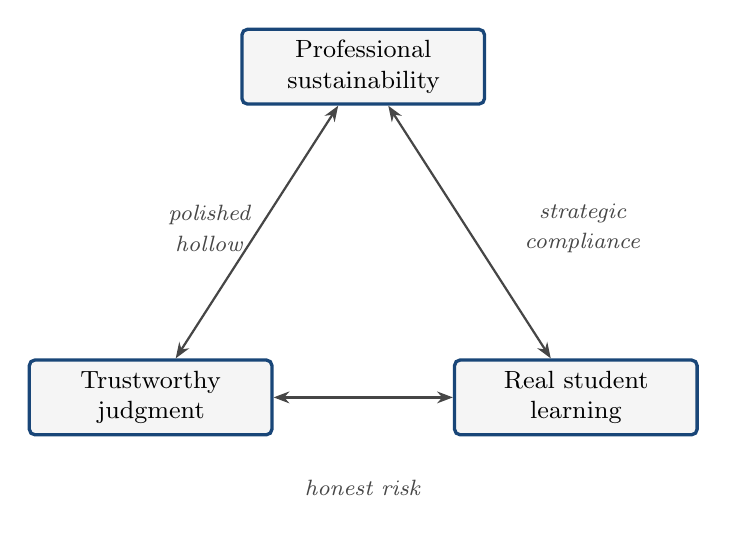
\begin{tikzpicture}
\node[emphasis-node, minimum width=3cm, minimum height=0.85cm, align=center, text width=2.8cm]
  (sustain) at (0, 2.8) {Professional\\sustainability};
\node[emphasis-node, minimum width=3cm, minimum height=0.85cm, align=center, text width=2.8cm]
  (judgment) at (-2.7, -1.4) {Trustworthy\\judgment};
\node[emphasis-node, minimum width=3cm, minimum height=0.85cm, align=center, text width=2.8cm]
  (learning) at (2.7, -1.4) {Real student\\learning};
\draw[bidir-arrow] (sustain) -- (judgment);
\draw[bidir-arrow] (sustain) -- (learning);
\draw[bidir-arrow] (judgment) -- (learning);
\node[caption-text, align=center, text width=2.8cm] at (-1.95, 0.75)
  {\footnotesize\textit{polished\\hollow}};
\node[caption-text, align=center, text width=2.8cm] at (2.795, 0.75)
  {\footnotesize\textit{strategic\\compliance}};
\node[caption-text, align=center, text width=2.8cm] at (0, -2.55)
  {\footnotesize\textit{honest risk}};
\end{tikzpicture}
\caption{\textbf{The Instructor's Trilemma.} Three commitments faculty hold in tension. Each edge labels the failure mode that arises when the two adjacent commitments are kept at the cost of the third. AI sharpens each edge; it did not create the trilemma. This mirrors the Student's Trilemma in \cref{fig:honest-a-bind}.}
\label{fig:instructor-trilemma}
\end{figure}

\subsection{Three instructor failure modes}
\label{i:subsec:trilemma-failures}

\textit{Sustainability and trustworthy judgment without student learning.} The instructor maintains a manageable workload and grades that can be defended in conversation, but the pedagogy itself has hollowed out. Assignments become defensive: in-class blue-book exams that limit AI use but also limit what can be assessed; multiple-choice tests that are easy to grade but reveal little; assignments rewritten until blind AI use ``collapses under its own weight'' \citep{samuel2025retrospective} but in the process becoming so constrained that students do not develop the kinds of thinking the course title promises. Call this the \keyterm[polished hollow!instructor]{instructor polished hollow}: the professional surface is intact, the integrity record is defensible, but the educational mission has hollowed out from inside.

\textit{Sustainability and student learning without trustworthy judgment.} The instructor protects their workload and produces actual student learning, but lets AI-assisted work into the grade book without demanding genuine ownership. AI grades the homework; students use AI to write the papers; the pedagogy may even be sophisticated and engaging; but the instructor can no longer defend in conversation what individual grades, recommendations, or evaluations actually signify. This is the \keyterm[strategic compliance!instructor]{instructor strategic compliance}: the instructor complies with the institutional appearance of credentialing function while quietly accepting that the verification was not done. This is the failure mode most common when the cost of demanding genuine ownership exceeds what the instructor can sustainably do.

\textit{Trustworthy judgment and student learning without sustainability.} The instructor holds high standards, refuses to lower expectations under AI pressure, redesigns assessments to surface genuine thinking, conducts the oral conversations and process audits the framework calls for, and produces real learning that students will carry with them. And burns out. The literature names this pattern directly in its observable forms: faculty reverting to blue books or opting for early retirement to avoid the perceived flood of machine-generated text \citep{manturuk2026best}. Call this the \keyterm[honest risk!instructor]{instructor honest risk}: every commitment kept, no commitment surrendered, but the personal cost cannot be sustained.

The American Association of University Professors frames this pattern at the professional-labor level. They argue that the uncritical adoption of AI poses a threat to academic professions through work intensification and through implications for the faculty working conditions that affect student learning conditions \citep{aaup2025artificial}. The intensification is real: more policing time, more course redesign cycles, more individual policy invention. The honest-risk failure mode is the price an instructor pays for refusing the other two.

AI did not create the Instructor's Trilemma. The trilemma names a structural tension between commitments faculty have always held in some balance. What AI did was sharpen each edge. Each pair of corners is harder to hold together when AI assistance lowers the apparent cost of giving up the third.

\subsection{How the trilemma manifests differently by faculty type}
\label{i:subsec:trilemma-by-type}%
\index{adjunct faculty}%
\index{contingent faculty}%
\index{employment status}

The three corners are universal among teaching faculty, but the pull strength on each corner differs sharply by employment status. The dimension is unusually consequential in U.S. higher education: roughly two-thirds of the academic workforce is contingent, and roughly half is part-time adjunct \citep{aaup2025contingent}. The trilemma looks different depending on which contractual category the instructor occupies. Four types are worth distinguishing.

\textit{Tenured faculty with reasonable course loads.} These instructors have the most freedom across all three corners. Sustainability is relatively secure (the contract cannot be cancelled at the end of the semester), trustworthy judgment is supported by long-developed disciplinary reputation, and student learning can be pursued through whichever pedagogical experiments the instructor finds compelling. The honest-risk failure mode is the failure they can most afford and that they sometimes consciously choose: holding high standards even at significant personal workload cost. They may also be the most likely to romanticize the honest-risk posture in advice they give to junior colleagues for whom it is genuinely unsustainable.

\textit{Tenure-track faculty.}\index{tenure-track faculty} Professional sustainability dominates because the tenure case is at stake, and almost every classroom decision feeds eventually into the tenure dossier. Course evaluations matter; student complaints carry weight; pedagogical experiments that backfire can be remembered. The polished-hollow failure mode is the most relevant risk: defensive pedagogy that protects the tenure case by avoiding controversy, at the cost of actual learning. The framework provides an alternative path through better-designed assignments and clearer rubrics, but the structural pressure toward defensiveness is real and should be acknowledged. The fear is not imagined, and it has been measured. In a randomized comparison in introductory physics, with identical content and handouts, passive sections taught by experienced and highly rated lecturers, and an instructor who made no attempt to sell either method, students in the active sections learned more and rated their own learning lower \citep{deslauriers2019measuring}. The rating was still positive. It was just lower than for the polished lecture. The authors draw the conclusion that matters here: evaluating teaching by how much students feel they learned can quietly reward the weaker method. A course evaluation is evidence about the experience. It is not evidence about the learning, and an instructor defending a pedagogical choice can now say so with a citation.

\textit{Full-time non-tenure-track faculty}\index{lecturers}\index{workload} (lecturers, clinical faculty, teaching-stream professors, professors of practice). These positions have grown substantially in U.S. higher education and now constitute a meaningful share of teaching capacity. The trilemma is mixed: contract renewal pressure exists but is less acute than for adjuncts; teaching effectiveness is usually the explicit evaluation criterion (which protects the real-learning corner); but workload is often heavy and infrastructure for trustworthy judgment can be thin. Strategic compliance is a real risk when teaching loads exceed what allows for genuine verification of every student's work.

\textit{Adjunct and per-course contingent faculty.}\index{adjunct faculty!verification labor}\index{contingent faculty!structural failure mode} For this category, professional sustainability is dominant in a way that should not be moralized. An adjunct teaching four or five sections across two or three institutions cannot complete the time-intensive verification work the trustworthy-judgment corner requires. This is not a failure of values. The structural conditions of the role make it impossible. The strategic-compliance failure mode is the failure they most often inhabit, often without having meaningfully chosen it. For instructors in this position, the lowest-effort design in \cref{sec:evidence-of-thinking} is the relevant one: shift the grade onto in-person assessment and let homework carry little weight. It adds almost none of the verification labor the other models require, which is what the structural conditions of the role demand. \textbf{Honest risk is a luxury good\index{honest risk!who can afford it} in the academy:} only faculty whose positions permit it can consistently afford to take it. Recommendations in this Part that assume an instructor can spend extra time on oral defenses, individualized feedback, and process audits should be read with this constraint in mind. Institutional change that does not address the underlying labor conditions will leave contingent faculty trapped in a failure mode that is structural, not personal.

These four types are not comprehensive. Graduate-student instructors, postdoctoral teaching fellows, and emeriti returning to teach face the trilemma with their own type-specific pull patterns. Discipline also matters. Faculty in the humanities and writing-intensive fields face the trilemma in its most acute form, because their disciplines are where AI-generated text is hardest to distinguish from student work. Faculty in disciplines with strong oral and laboratory traditions have more natural defenses against the strategic-compliance pattern. The framework's value is that the corners stay the same; what changes is the relative pull and the failure mode most likely to materialize given an individual instructor's structural conditions.

\subsection{Why the Instructor's Trilemma matters for the rest of this Part}
\label{i:subsec:trilemma-stakes}

The instructor's version of the student's navigation rule is the same in spirit: when one corner starts to slip, adjust what you assign and how you grade rather than abandon the corner.

The assessment models, design patterns, integrity procedures, and faculty-development approaches developed in the rest of this Part are tools for holding the three corners of the trilemma together under AI pressure. The three assessment models (Oral-Defense, Evidence-of-Thinking, Hybrid) are designed to make trustworthy judgment achievable at different course sizes without requiring the honest-risk personal cost. The CAT framework's four assignment categories are designed to align with both faces of student learning (cognitive development and workforce preparation) rather than forcing instructors to choose. The fair response sequence for suspected misuse is designed to protect against the policing exhaustion that drives the honest-risk failure mode.

Without the trilemma frame, the operational tools in this Part can read as a list of best practices. With it, they read as coordinated commitments that protect the instructor from each of the three failure modes simultaneously. The faculty discourse on AI is currently dominated by individual instructors describing whichever failure mode they are personally most worried about. The framework's value is that it surfaces the structure beneath the individual stories and gives instructors a vocabulary for understanding why their colleagues are choosing different responses to the same forces.

\section{Three design axes: class size, level, and discipline}
\label{i:sec:three-axes}%
\index{class size}\index{course level}\index{discipline overlays}

The design choices an instructor makes about AI in a course are governed mostly by three dimensions: class size, course level, and discipline. The three are roughly independent, though level and size correlate in practice, since graduate courses tend to be smaller. Each still drives a different family of decisions, and treating them as a single axis (often labelled informally as ``undergraduate versus graduate'') tends to bury the design logic that this Part is meant to make visible. The three axes are summarized in \cref{tab:three-axes} and discussed in turn.

\begin{table}[ht]
\centering
\caption{\textbf{The three design axes.} Each axis drives a different family of decisions for AI-aware course design. Treating them together produces clearer choices than treating ``undergraduate versus graduate'' as a single axis.}
\label{tab:three-axes}
\begin{tabularx}{\textwidth}{>{\raggedright\arraybackslash}X >{\raggedright\arraybackslash}X >{\raggedright\arraybackslash}X}
\toprule
\textbf{Axis} & \textbf{Drives} & \textbf{Sections in this Part} \\
\midrule
Class size & \emph{How} you assess: which assessment model is feasible. & Oral-Defense Model (\cref{i:sec:oral-defense-model}); Evidence-of-Thinking Model (\cref{i:sec:evidence-model}); Hybrid Model (\cref{i:sec:hybrid-model}). \\
\addlinespace
Course level & \emph{What} you assess and how much AI autonomy to grant: Core Competence definition, the typical assignment-category mix, expected verification capacity. & Four assignment categories (\cref{i:sec:assignment-categories}); rubrics (\cref{i:sec:rubrics}). \\
\addlinespace
Discipline & The specifics of \emph{how} AI fits in: what verification looks like, what AI tools are appropriate, what counts as acceptable use. & Discipline overlays (\cref{i:sec:discipline-overlays}). \\
\bottomrule
\end{tabularx}
\end{table}

\textit{Class size} determines what direct contact the instructor (or trained TAs) can have with each student. A 12-person seminar can support oral defenses on every major assignment; a 200-person lecture cannot. This axis is the primary driver of which of the three assessment models discussed below fits the course. Class size does not, by itself, determine \emph{what} students should be able to do without AI.

\textit{Course level} determines the substance of Core Competence, the typical assignment-category mix, and how much AI autonomy a student can responsibly handle; \cref{i:subsec:category-by-level} develops the shift in detail.

\textit{Discipline} determines the specifics of verification and AI use. A mathematics assignment is verified by checking limits, units, and edge cases; a humanities essay is verified by checking primary sources, quotation accuracy, and argument structure; a programming assignment is verified by writing test cases. The framework is uniform across disciplines, but the verification practices, AI tool choices, and category boundaries are not. Discipline overlays in \cref{i:sec:discipline-overlays} address these specifics.

The three axes are largely independent. A small graduate seminar and a small first-year writing class share the assessment-model options that small classes support, but differ in category mix and AI autonomy. A large introductory mathematics class and a large introductory humanities class share the model constraints that large classes impose, but differ in what verification looks like. A large advanced seminar (rare but real) and a small introductory course share neither directly, and instructors in those settings can mix elements from different parts of this Part rather than picking one prepackaged path.

This Part is organized around all three axes. The CAT framework and the four assignment categories that follow are level-agnostic and discipline-agnostic at the framework level; their operational application varies along all three axes. The three assessment models that follow vary primarily by class size. The discipline overlays vary by discipline. Where the prose in this Part says ``a graduate course'' or ``an advanced undergraduate course,'' the relevant claim is usually about course level, and sometimes about class size, since graduate courses are typically smaller. The prose attempts to be precise about which.

\chapter{The Framework and Assignment Design}
\label{i:ch:the-framework-and-assignment-design}%

The design choices in this Part assume something they cannot supply: a student who wants to learn. A well-built assignment makes thinking visible and gives AI less to offload, but it cannot make a student care, and a student who does not care will route around the best task you can write. The deepest lever an instructor holds is not the assignment but the student's reason to engage with it. Design protects and rewards the will to learn; it does not create it. That comes earlier, from the case the instructor makes for the work: when students believe the reasoning they are building will outlast the answers and matter in the work they go on to do, they will spend effort a chatbot would spare them.

Buy-in has a condition that is easy to miss. Productive struggle happens only where it feels safe. A student who fears that a wrong first attempt will count against them will reach for the answer that removes the risk, and AI supplies it instantly. Lowering the stakes on early attempts, grading effort before correctness, and treating a wrong step as part of learning rather than a verdict make the struggle survivable, and a struggle that feels survivable is one students will actually attempt. Whether buy-in can be built deliberately has been studied. \Cref{i:sec:assignment-design} carries what the evidence supports.

\section{The CAT framework}
\label{i:sec:cat-framework}%
\index{CAT framework}

This guide uses the CAT framework: \keyterm[CAT framework!Core Competence]{Core Competence}, \keyterm[CAT framework!AI-assisted Practice]{AI-assisted Practice}, and \keyterm[CAT framework!Trustworthiness]{Trustworthiness}. The framework generalizes a three-axis assessment model originally developed for graduate mathematics, where independent mathematical understanding, AI-augmented skill, and epistemic responsibility are assessed separately. The Preface (page~\pageref{sec:foreword}) explains the lineage; Appendices~\ref{app:gmip} and~\ref{app:mae} present the original graduate-mathematics formulation in technical detail for instructors who want it.

\begin{description}
\item[Core Competence.] What students must understand and be able to do without AI or with tightly bounded assistance.
\item[AI-assisted Practice.] What students can do when they use AI responsibly as a permitted tool for learning, revision, analysis, coding, feedback, or exploration, without losing control of the work.
\item[Trustworthiness.] How well students verify, disclose, critique, and take ownership of AI-assisted work.
\end{description}

A course should assess all three dimensions, but not always with equal weight. A foundational course may emphasize Core Competence. A capstone course may place more weight on AI-assisted Practice and Trustworthiness. A professional course may emphasize judgment, privacy, and defensible decisions.

The framework is consistent with UNESCO guidance that treats AI competence as part of a human-centered educational system rather than a substitute for teacher and learner agency \citep{miao2024aib,miao2024aia}. It has one non-negotiable feature: AI skill should not compensate for failure to meet the core learning goals of the course. A student who can produce strong AI-assisted work but cannot explain the central ideas has not met the same standard as a student who understands the material.

\subsection{Core Competence}
\label{i:subsec:core-competence}

Core Competence is the part of the course that remains the student's own. It may include definitions, methods, concepts, interpretations, calculations, source analysis, writing decisions, experimental reasoning, coding fundamentals, design principles, or ethical judgment.

Each instructor should identify the core explicitly. The useful question is not, ``Can AI do this task?'' The useful question is, ``What must students still be able to do when AI is unavailable, inappropriate, or untrustworthy?''

Core Competence can be assessed through no-AI quizzes, in-class writing, oral explanations, lab practicals, live coding checks, source-analysis exercises, design critiques, short exams, or closed-resource problem solving. These assessments need not dominate the course, but they should be meaningful.

\subsection{AI-assisted Practice}
\label{i:subsec:ai-augmented-practice}

AI-assisted Practice is the student's ability to use AI productively without losing control of the work. This includes asking useful questions, constraining a model, comparing explanations, testing code, finding flaws, improving drafts, generating examples, and using AI feedback to improve human reasoning.

This is not a lesser skill. In many fields, responsible use of AI will become part of professional competence. Students should learn it in courses where faculty can set boundaries and provide feedback.

The instructor's task is to design assignments where AI use is visible and assessable. A strong AI-integrated assignment asks students not only for a final product, but also for evidence of choices, verification, revision, and judgment.

\subsection{Trustworthiness}
\label{i:subsec:responsible-judgment}

Trustworthiness includes verification, disclosure, privacy, source discipline, and intellectual ownership. It is the dimension that prevents AI use from becoming laundering: taking generated output and presenting it as independent understanding.

A student's responsible judgment is visible when they can answer questions such as these:

\begin{itemize}
\item What did AI contribute?
\item What did you accept, reject, or revise?
\item How did you check the output?
\item What sources did you verify yourself?
\item What part of the submitted work can you explain without AI?
\end{itemize}

These questions are useful across disciplines. They apply to a proof, a policy memo, a lab report, a design prototype, a literature review, a computer program, and a close reading of a text.

\section{Four assignment categories}
\label{i:sec:assignment-categories}%
\index{assignment categories}

Every assignment should tell students what role AI may play. The guide uses four categories: NAI, AIT, AIC, and AIS. The categories are simple enough for a syllabus, but flexible enough for different disciplines (\cref{fig:assignment-color-tree}). These are the same four categories students meet in Part~\ref{part:student}, framed here for the instructor designing and labeling assignments; readers coming from Part~\ref{part:student} can move quickly through the definitions and focus on the design guidance. External guidance points the same way: the 2026 HEPI survey recommends that institutions offer AI-free assessments alongside assessments that expect students to use AI \citep{stephenson2026student}, which is the NAI-versus-AIC distinction stated as institutional advice.

Before applying these categories, instructors may want to recommend that students complete the AI account configuration template in Part~\ref{part:student} (\cref{app:ai-config}) at the start of the course. The configuration step takes ten minutes, calibrates the AI to the student's level and discipline, and creates a written record of the use boundaries the student has committed to. For a course with significant AIC-category work, requiring the configuration as a no-credit first assignment is a low-cost way to start the term with shared expectations.

\begin{figure}[ht]
\centering
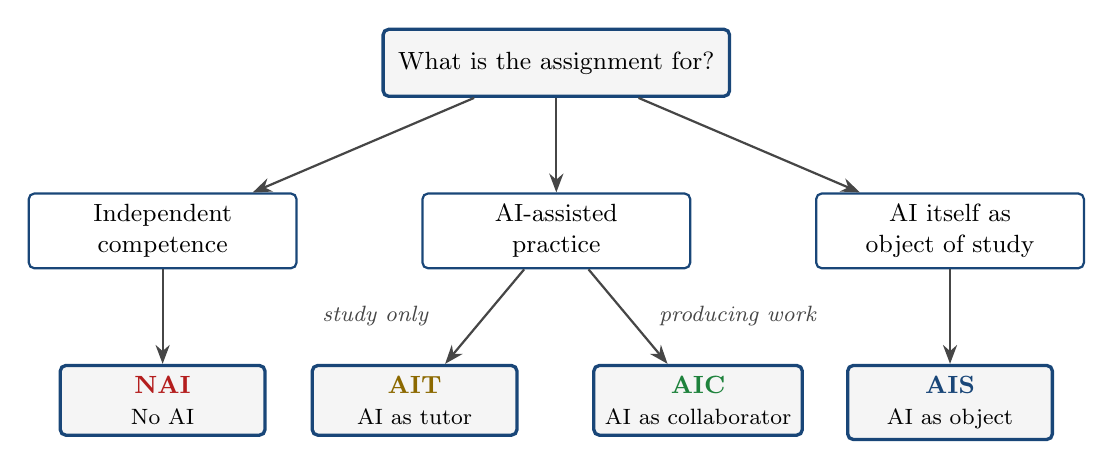
\begin{tikzpicture}[node distance=0.4cm and 0.7cm, every node/.style={font=\small}]
% Root question
\node[emphasis-node, minimum width=4.4cm, minimum height=0.85cm] (root) {What is the assignment for?};

% Level 1: Core Competence vs. AI-assisted Practice vs. AI itself
\node[framework-node, below=1.2cm of root, xshift=-5cm, minimum width=3.4cm, minimum height=0.85cm] (core) {Independent\\competence};
\node[framework-node, below=1.2cm of root, minimum width=3.4cm, minimum height=0.85cm] (ai-aug) {AI-assisted\\practice};
\node[framework-node, below=1.2cm of root, xshift=5cm, minimum width=3.4cm, minimum height=0.85cm] (ai-obj) {AI itself as\\object of study};

% Level 2: leaf categories
\node[emphasis-node, below=1.2cm of core, minimum width=2.6cm, minimum height=0.85cm, fill=lightgray] (red) {\textcolor{catNAI}{\textbf{NAI}}\\\footnotesize No AI};
\node[emphasis-node, below=1.2cm of ai-aug, xshift=-1.8cm, minimum width=2.6cm, minimum height=0.85cm, fill=lightgray] (yellow) {\textcolor{catAIT}{\textbf{AIT}}\\\footnotesize AI as tutor};
\node[emphasis-node, below=1.2cm of ai-aug, xshift=1.8cm, minimum width=2.6cm, minimum height=0.85cm, fill=lightgray] (green) {\textcolor{catAIC}{\textbf{AIC}}\\\footnotesize AI as collaborator};
\node[emphasis-node, below=1.2cm of ai-obj, minimum width=2.6cm, minimum height=0.85cm, fill=lightgray] (blue) {\textcolor{catAIS}{\textbf{AIS}}\\\footnotesize AI as object};

% Connections root → level 1
\draw[flow-arrow] (root) -- (core);
\draw[flow-arrow] (root) -- (ai-aug);
\draw[flow-arrow] (root) -- (ai-obj);

% Connections level 1 → leaves
\draw[flow-arrow] (core) -- (red);
\draw[flow-arrow] (ai-aug) -- (yellow);
\draw[flow-arrow] (ai-aug) -- (green);
\draw[flow-arrow] (ai-obj) -- (blue);

% Branch labels
\node[caption-text, font=\footnotesize\itshape] at ($(ai-aug)!0.5!(yellow) + (-1.4,0)$) {study only};
\node[caption-text, font=\footnotesize\itshape] at ($(ai-aug)!0.5!(green) + (1.4,0)$) {producing work};
\end{tikzpicture}
\caption{\textbf{Choosing the assignment color.} The instructor decides what the assignment is for, then selects a color that matches that purpose. \NAI{} (No AI) protects independent competence; \AIT{} (AI as Tutor) allows AI for study support but not for submitted work; \AIC{} (AI as Collaborator) permits responsible AI use in producing the submission; \AIS{} (AI as Object of Study) makes AI itself the subject of analysis. The choice should appear on the assignment.}
\label{fig:assignment-color-tree}
\end{figure}

\subsection{\texorpdfstring{\NAI{}: No AI}{NAI: No AI}}
\label{i:subsec:red}

NAI assignments prohibit AI use. They are used to assess Core Competence.

NAI assignments take familiar forms: in-class exams, short quizzes, oral explanations, live coding, lab practicals, handwritten derivations, in-class writing. What makes an assignment NAI is not the format but the declared purpose: each is a stated, protected measurement of what the student can do alone.

A NAI assignment should have a clear reason. It should not be a default expression of distrust. The reason is usually that the instructor needs evidence of what the student can do without outside help.

\subsection{\texorpdfstring{\AIT{}: AI as Tutor}{AIT: AI as Tutor}}
\label{i:subsec:yellow}

AIT assignments allow AI for study support, but not for producing submitted work. Students may use AI to ask for hints, examples, explanations, practice questions, or feedback before doing the work themselves.

AIT rules are useful when the instructor wants students to benefit from tutoring while still submitting independent work. A homework set might be AIT if students may ask AI to explain a concept but may not ask it to solve the assigned problems.

For AIT assignments, instructors may define a help ladder that structures the order in which AI assistance is permitted: concept explanation, then an analogous example, then one hint on the assigned problem, then a critique of the student's attempt, and only then a full solution for ungraded practice. The ladder allows substantial AI support while protecting retrieval practice and productive struggle. Students who begin with a full solution to the assigned problem skip every learning move the assignment was designed to produce.

\subsection{\texorpdfstring{\AIC{}: AI as Collaborator}{AIC: AI as Collaborator}}
\label{i:subsec:green}

AIC assignments allow AI as part of the working process. Students may use AI to brainstorm, revise, debug, critique, summarize, generate alternatives, or test ideas. AIC assignments require disclosure and verification.

AIC assignments work best when the process matters. For example, a student might submit an original plan, selected AI interactions, a revised product, and a verification note. The final product may be stronger because AI was used, but the student's judgment remains visible.

\subsection{\texorpdfstring{\AIS{}: AI as Object of Study}{AIS: AI as Object of Study}}
\label{i:subsec:blue}

AIS assignments make AI itself part of the subject. Students might critique an AI-generated essay, identify hallucinated citations, repair flawed code, compare model responses, evaluate bias, or analyze how a tool handles a disciplinary problem.

AIS assignments are especially valuable because they teach students not to treat AI as an oracle. They make error detection and tool critique explicit learning goals. That critique goes deeper when students know why the errors sound certain, since a system graded only on answers has no reason to say it does not know \citep{kalai2025hallucinate}.

\subsection{The categories and the AI Assessment Scale}
\label{i:subsec:aias-crosswalk}%
\index{AI Assessment Scale}\index{assignment categories!AI Assessment Scale crosswalk}

These four categories are not the only way to label AI use. The best known alternative is the AI Assessment Scale, five ordered levels running from no AI to open exploration \citep{perkins2024aias}. It has been translated into thirty languages and used in over three hundred institutions, and Australia's tertiary education regulator has named it as one tool for marking where AI belongs in an assessment. A pilot at one university reported a drop in AI-related misconduct cases after adoption \citep{furze2024aias}. The authors revised the scale in 2025 \citep{perkins2025reimagining}.

The categories here add two things. The scale's middle levels are set by what the AI does, whether it plans, drafts, or completes. AIT is set by whether AI output enters the submission at all. That is a line an instructor can state and a student can check. AIS sits outside the scale. All five levels answer one question, how much AI a student may use, and AIS asks what the AI is doing.

The scale exists because a two-valued rule, allowed or banned, is too coarse for what students actually do. The same criticism is often aimed at any permission framework, including this one. It does not land. Three of these categories differ only in how much assistance an assignment permits. The fourth asks something else, which is what the AI itself can be trusted to do.

A department already using the scale does not have to choose. NAI matches Level 1. AIT matches Level 2, with AI text kept out of what is handed in. AIC covers Levels 3 and 4, where AI work enters the submitted product. Level 5 asks students to build new AI applications, which is near AIS but not the same. That mapping is to the 2025 scale, which renumbered its levels.

The scale does some things better. Five levels are finer than the three that sit on the light. It is peer reviewed, revised, translated, and adopted at scale, and these categories are none of those yet. Fewer categories buy compliance and cost precision. That is the trade.

The revised scale dropped its traffic-light colors so its levels would not read as a ranking. The light here ranks nothing beyond how much AI an assignment allows, which is why AIS sits off it in blue. The authors of the revision note that a red-to-green light still earns its place where clarity matters most.

\subsection{A syllabus table for assignment categories}
\label{i:subsec:category-table}

\begin{center}
\begin{tabular}{p{0.13\textwidth}p{0.24\textwidth}p{0.53\textwidth}}
\toprule
\textbf{Category} & \textbf{AI role} & \textbf{Typical purpose} \\
\midrule
\NAI{} & No AI & Measure independent competence. \\
\AIT{} & Tutor only & Support study while preserving independent submitted work. \\
\AIC{} & Collaborator & Teach responsible AI-assisted work with disclosure and verification. \\
\AIS{} & Object of study & Teach critique of AI output, bias, errors, and limits. \\
\bottomrule
\end{tabular}
\end{center}

\subsection{Category mix shifts with course level}
\label{i:subsec:category-by-level}

The four categories are level-agnostic at the framework level; any assignment in any course can fall into any of the four. The \emph{typical mix}, however, shifts substantially with course level, and ignoring this shift is one of the more common ways instructors design AI policy poorly.

Introductory courses typically lean toward NAI and AIT. The reason is not distrust. The reason is that students at this level have not yet built the disciplinary competence required to verify AI output reliably. Granting AIC-category latitude before that competence exists can amount to inviting students to accept work they cannot evaluate. A Calculus 1 student cannot distinguish a correct optimization solution from a confidently wrong one; a first-year writing student cannot reliably detect when an AI revision has shifted the meaning of a thesis. \NAI{} protects the foundational skill; \AIT{} lets the AI act as a study companion without entering the submitted work. When introductory courses do assign verification, the instructor supplies the target: a benchmark, a special case, a source to check against, or the method to use. The task then teaches checking rather than presuming it. The seeded-error check in \cref{i:subsec:seeded-error-check} is built on this principle.

Intermediate undergraduate courses typically use a balanced mix. As students develop disciplinary competence, the verification side of AIC-category work becomes feasible, and AIS-category critique becomes possible. A junior-level course in any discipline can typically support meaningful AIC and AIS assignments alongside NAI and AIT ones.

Advanced undergraduate and graduate courses typically lean toward AIC and AIS. Students at this level can verify AI output, can defend submitted work in detail, and can engage AI tools as objects of disciplinary critique. NAI assignments still serve a purpose at this level (foundational-skills demonstrations, qualifying-exam preparation), but they are typically a smaller fraction of the course.

The shift is not strictly linear with level: a research-methods graduate seminar might sensibly require several NAI oral examinations, while an upper-division undergraduate elective might be almost entirely AIC. The shift is also not driven by class size: a 200-student introductory lecture and a 12-student introductory seminar share the typical NAI/AIT weighting; a small graduate seminar and a large graduate-equivalent course share the typical AIC/AIS weighting. Enrollment motive is a third variable. Students choose an elective and are placed in a requirement, and that difference in why they are there shapes what a course can ask of them, independent of level, size, and field.

A useful rule for an instructor designing a course: the Core Competence (NAI and AIT assessments) defines what the course is for; the AI-assisted Practice (AIC) and AI-as-object (AIS) work defines how that competence is exercised in a tools-rich environment. The proportion between these two halves is what shifts with course level. \Cref{i:app:syllabus} gives syllabus language ready to adapt, and \cref{i:app:assignment-label} gives a label template for individual assignments.

\section{Designing assignments that preserve thinking}
\label{i:sec:assignment-design}%
\index{assignment design}\index{buy-in, student}\index{buy-in, student!and safety to be wrong}\index{productive struggle}

The best AI-aware assignments make student thinking visible. They do not merely ask for a final answer. They ask for evidence of how the student framed the problem, what they tried first, what they asked AI, what they checked, and how the final work changed.

A randomized controlled trial of an AI-tutoring system in an introductory physics course at Harvard built its design around seven practices: active engagement, cognitive-load management, growth mindset, scaffolding, feedback accuracy, timely targeted feedback, and self-pacing \citep{kestin2025ai}. The evidence behind them is not uniform. Active engagement rests on a meta-analysis of 225 studies \citep{freeman2014active}, feedback on a literature going back decades \citep{black1998assessment,hattie2007power}, and cognitive load on a developed theory \citep{sweller2011cognitive}. The seven are useful as a design checklist. They are not seven equally settled findings.

The seven practices map onto principles long established in the learning-science literature \citep{ambrose2010how,nationalacademies2018how}. Active engagement in particular rests on a large empirical base in undergraduate STEM: a meta-analysis of 225 studies found that active-learning approaches raised examination performance by 0.47 standard deviations, with students under traditional lecturing 1.5 times more likely to fail than those under active learning \citep{freeman2014active}. The cognitive-load principle is developed in detail in the synthesis by \citet{sweller2011cognitive}. The first five practices can be built into any assignment whether or not it uses AI; the last two are easier when AI is part of the design.

\index{Kestin AI-tutor study}In Kestin's specific implementation (described in more detail in Part~\ref{part:student} \cref{sec:evidence-limits}), the AI tutor's system prompt handled the first three practices, the platform's structured walkthrough handled scaffolding, accuracy came from worked solutions loaded in advance, and only the last two are properties of AI as a medium. The assignment patterns recommended in this section are consistent with all seven, and instructors who want a deeper grounding for these patterns can read the Kestin study directly. A separate field experiment in high-school mathematics provides the converse evidence. An unrestricted AI interface that simply answered questions produced 48\% practice gains but 17\% exam losses. A guardrailed variant designed to give hints rather than answers produced 127\% practice gains and no exam loss \citep{bastani2025generative}. The design choice behind the difference is what the AIT assignment category in this guide formalizes: AI is permitted as a hint-giver, not as a solver. The guardrailed tutor also had the worked solutions in its prompt, which is what kept it from inventing answers. Both halves matter. A tutor told to give hints, with no answer key behind it, gives confident hints toward the wrong place.

\index{buy-in, student!evidence for}\index{relevance, writing about}%
One approach to buy-in has been tested directly. Hulleman and Harackiewicz randomly assigned high-school science students to write briefly about how a topic connected to their own lives, against a control group that wrote summaries of the same material \citep{hulleman2009promoting}. Students who did not expect to do well earned higher grades and reported more interest in science. Students who already expected to do well showed no difference. Canning and colleagues ran the same design across three units of a college introductory biology course and found higher grades, higher continuation into the second course, and higher persistence in the major \citep{canning2018improving}. Both studies come from one research program rather than from independent groups, and reported effects in this literature range from none to large, so this is a promising design and not a settled result.

The AI question here is sharper than it looks. The assignment asks a student to write about why the material matters to them. A chatbot will produce that in seconds and it will read well. The whole mechanism depends on the student making the connection. An AI-written version is not a weaker dose of the intervention. It is the absence of it, wearing its clothes.

A separate concern is the social dimension of learning. A study of generative AI's effect on peer interactions in computing courses found that students increasingly route their questions to AI rather than to each other, and that students seeking peer help are sometimes redirected to AI rather than receiving it \citep{hou2025roads}. The pattern erodes the study groups, peer tutoring, and informal collaborative practices through which much undergraduate learning has historically happened, including the peer-instruction methods documented to improve conceptual understanding in undergraduate STEM \citep{mazur1997peer}. Assignments designed to preserve thinking should preserve named peer interaction as one of the things they preserve.

A useful design pattern is the \keyterm[Plan-Use-Verify]{plan--use--verify} structure (\cref{fig:plan-use-verify}). The structure operationalizes the principle, well established in the learning sciences, that learners benefit from explicit self-monitoring before and after task engagement \citep{nationalacademies2018how}.

\begin{description}
\item[Plan.] Before using AI, the student writes a short plan, prediction, outline, proof sketch, lab strategy, or source note.
\item[Use.] The student uses AI within the assignment rules and records the relevant interaction.
\item[Verify.] The student checks the output and explains what was accepted, changed, rejected, or corrected.
\end{description}

\begin{figure}[ht]
\centering
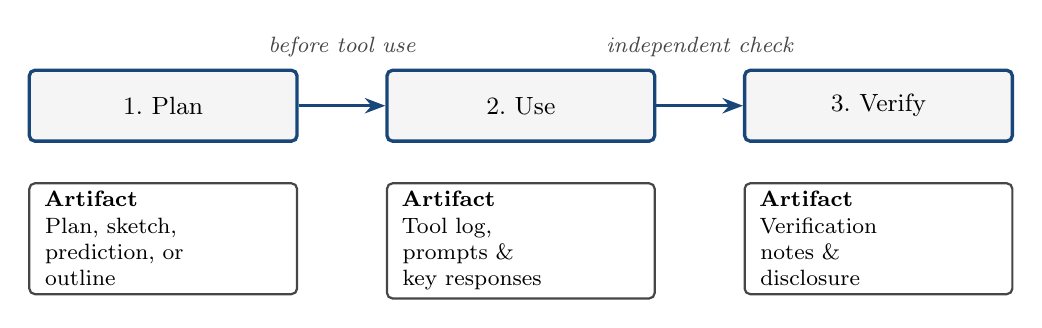
\begin{tikzpicture}[node distance=0.4cm and 1.1cm, every node/.style={font=\small}]
% Three stages
\node[emphasis-node, minimum width=3.4cm, minimum height=0.9cm] (plan) {1.~Plan};
\node[emphasis-node, right=of plan, minimum width=3.4cm, minimum height=0.9cm] (use) {2.~Use};
\node[emphasis-node, right=of use, minimum width=3.4cm, minimum height=0.9cm] (verify) {3.~Verify};

% Artifact under each stage
\node[secondary-node, below=0.5cm of plan, minimum width=3.4cm, minimum height=1.3cm, align=left, text width=3.0cm]
  {\footnotesize\textbf{Artifact}\\
   \footnotesize Plan, sketch,\\
   \footnotesize prediction, or\\
   \footnotesize outline};
\node[secondary-node, below=0.5cm of use, minimum width=3.4cm, minimum height=1.3cm, align=left, text width=3.0cm]
  {\footnotesize\textbf{Artifact}\\
   \footnotesize Tool log,\\
   \footnotesize prompts \&\\
   \footnotesize key responses};
\node[secondary-node, below=0.5cm of verify, minimum width=3.4cm, minimum height=1.3cm, align=left, text width=3.0cm]
  {\footnotesize\textbf{Artifact}\\
   \footnotesize Verification\\
   \footnotesize notes \&\\
   \footnotesize disclosure};

% Forward arrows
\draw[emphasis-arrow] (plan) -- (use);
\draw[emphasis-arrow] (use) -- (verify);

% Labels above arrows
\node[caption-text, above=0.5cm] at ($(plan)!0.5!(use)$) {\footnotesize before tool use};
\node[caption-text, above=0.5cm] at ($(use)!0.5!(verify)$) {\footnotesize independent check};
\end{tikzpicture}
\caption{\textbf{The Plan--Use--Verify assignment structure.} Each stage produces a small artifact the instructor can see. The three artifacts together show how the student thought, where AI helped, and what the student verified. Grading does not require reading every prompt; it requires seeing that all three stages happened.}
\label{fig:plan-use-verify}
\end{figure}

This structure does not require grading every prompt. It asks students to show enough of the process that the instructor can see whether learning occurred.

\subsection{Plan-Use-Verify in practice}
\label{i:subsec:plan-use-verify-practice}

The three artifacts work because each is short and gradable at a glance. The pattern is the same shape across disciplines, with only the lengths and content varying.

For a humanities essay, the Plan might be a one-paragraph thesis with the primary sources the student will use. The Use is a 3--5 line tool log naming what the student asked AI and what was returned in summary. The Verify is a 4--6 line note describing one place the student returned to a source to check an AI-suggested claim, plus what was accepted or rejected.

For a programming problem set, the Plan is a sketch of the algorithm or data structure the student intends to use, written before any code. The Use is the prompts and key responses from any AI debugging help, with the student's own diagnostic questions surfaced. The Verify is a list of test cases run, with one or two showing edge cases that catch a typical bug.

For a mathematics problem, the Plan is the student's setup of the problem (variables, constraints, choice of method) before AI use. The Use is a record of any AI hint or critique. The Verify is a unit check, a limiting-case check, or a comparison with a known result.

Three patterns make this work and three patterns break it.

\emph{Works when:}
\begin{itemize}
\item The three artifacts together are short, one page or less for most assignments. Brevity forces selection of the meaningful moves.
\item The artifacts are gradable at a glance, not parsed line-by-line. The instructor reads them as evidence of process, not as objects of grading.
\item The student treats the structure as a thinking aid. The Plan forces commitment before AI exposure; the Verify forces a check after.
\end{itemize}

\emph{Breaks when:}
\begin{itemize}
\item The artifacts are graded on length or completeness. Process documentation drifts into theater (\cref{i:subsec:scalable-evidence}).
\item The Plan is written after the work is finished. The pattern collapses into retroactive rationalization.
\item The instructor demands verbatim AI transcripts. The signal-to-noise ratio drops to near zero, and students learn to game the documentation rather than the work.
\end{itemize}

The pattern scales: same shape for a 1-page homework problem and for a semester project; only the lengths change. An instructor adopting Plan-Use-Verify across a course can keep the structural template constant and adjust expected lengths to the assignment.

\subsection{Writing the problem to start the spiral}
\label{i:subsec:spiral-problems}%

\index{problems, writing and recasting}\index{assignment design!recasting single-answer problems}\index{Learning Spiral!writing a problem to start it}Plan--Use--Verify wraps around a problem. The problem itself can do more of the work.

A problem written for a single answer is finished when the answer arrives. A student who reaches it has no reason to continue, and a student who cannot reach it has nowhere to go but the answer key or the AI. \AIT{} assignments make a third option available, because the student is allowed a tutor and the problem can be written on that assumption. The instructor sets the trajectory once, in the wording, and every student runs it.

The Learning Spiral (\cref{fig:learning-spiral}) supplies the shape: a question at the center, then try, ask, work, verify, and reflect. A problem can supply the first turn and hand the student the second.

\begin{quote}
\textbf{Single-answer form.} A car loan of \$18{,}000 is repaid monthly over four years at 6\% annual interest. Compute the monthly payment.
\end{quote}

\begin{quote}
\textbf{Spiral form.} A car loan of \$18{,}000 is repaid monthly over four years at 6\% annual interest.
\begin{enumerate}
\item Before computing anything, estimate the monthly payment and write one sentence saying what your estimate assumes.
\item Compute it.
\item If your estimate was off by more than twenty percent, ask an AI tutor what your reasoning missed. Ask for the flaw, not the payment.
\item Check the computed figure a second way.
\item Predict, before computing, what changes if the term is six years instead of four. Say whether the total interest paid roughly doubles, and why.
\end{enumerate}
\end{quote}

The arithmetic is identical. What changed is that the student now has somewhere to go when stuck, a reason to keep going after the answer arrives, and a question at the end that the first version never raised. The AI is present in step three and is asked for a diagnosis rather than a result, which is what the \AIT{} category is for.

This is also the cheapest way to refresh a problem set. Recasting an old problem this way produces a genuinely new assignment even when the underlying computation is unchanged, and it does not depend on inventing a new scenario every term. An instructor with a bank of single-answer problems has the raw material already.

\index{Polya@P\'olya, George}The closing step has a long history. Asking what a solved problem opens goes back at least to P\'olya's \emph{How to Solve It} \citep{polya1945solve}. The companion repository extends this recast into a method any course can run, with worked before-and-after pairs from a writing course, a data course, and a first-year lab, and a repertoire of closing questions in that tradition (\texttt{companion/spiral-problems/}).

\subsection{Required mentor prompts}
\label{i:subsec:required-mentor}%
\index{mentor prompt!required}

Some assignments benefit from a course-level requirement that students begin AI use with a mentor prompt. The pattern is most useful in AIT-category assignments and in introductory courses where verification competence is still developing. The mentor prompt itself is described in Part~\ref{part:student} (\cref{subsec:mentor-prompt}) from the student's perspective; this subsection treats it as an instructor design choice.

Why require what students should ideally do on their own? The same reason any scaffold is required in a course: not every student arrives with the habits a self-directed learner would have, and building those habits explicitly is often more effective than expecting students to develop them on their own under assignment pressure. A required mentor prompt at the start of an assignment makes scaffolded AI use the default rather than an option students may or may not exercise.

The required mentor prompt is most useful when paired with the thread-review practice developed in \cref{i:sec:integrity}. The sampling guidance in that section (three to four threads per assignment, chosen at random or based on signal) applies directly. Used together, the required mentor prompt and the thread-review practice operationalize the AIT category: AI is permitted, the form of AI use is scaffolded, and the instructor can see what students are actually doing.

Different disciplines call for slightly different mentor prompts. In Calculus I, the mentor prompt should emphasize verification of intermediate algebraic steps: students with weak prerequisite skills are particularly at risk of accepting AI solutions they cannot themselves derive, and the mentor's job is to surface the gap rather than paper over it. In first-year writing, the mentor prompt should emphasize asking the student what they are trying to argue before suggesting language: AI that drafts before the student has clarified their own thinking can produce prose that displaces the student's voice without their noticing. In introductory programming, the mentor prompt should emphasize having the student narrate the algorithm before requesting code: students who skip the design step often produce working code they cannot explain or extend. In introductory statistics, the mentor prompt should emphasize verifying that an AI-supplied test or formula matches the problem's assumptions: students often accept a confident answer without checking whether the test's preconditions are met. In physics problem sets, the mentor prompt should emphasize identifying which principle or law applies before computation begins: AI-supplied solutions often produce algebraically valid work from a wrongly-identified starting point.

An important case for instructors to watch for is the student who has strong tool-use skill but weak learning-with-AI skill (the two skills introduced in Part~\ref{part:student}, \cref{sec:two-skills}). These students will produce clean prompts and clean outputs and will look competent in routine assessment. They will fail under transfer questions and under in-class no-AI work. The required mentor prompt does not solve this case, but it makes it easier to detect, because the mentor's calibration step surfaces the gap that the student's tool-use fluency would otherwise hide.

Honest acknowledgment: students will engage performatively with a required mentor prompt. Some will run through the calibration questions in a perfunctory way and then defect to a different AI session for the real work. Performative engagement is still better than no engagement, but it is not full engagement, and instructors should not expect the required mentor prompt to fully solve the problem it is designed to address. Thread review, occasional in-class no-AI assessment, and the Plan-Use-Verify pattern from \cref{i:subsec:plan-use-verify-practice} together do more than any one of them alone.

The pattern is offered as a recommendation, not a default. Courses where students already have well-developed learning-with-AI skill (typically advanced undergraduate and graduate courses) may find a required mentor prompt more friction than benefit. Introductory courses, and courses where the student population shows the high-tool-use and low-learning-with-AI pattern, are the strongest candidates.

\subsection{Platform-specific implementation}
\label{i:subsec:platform-implementation}%
\index{ChatGPT}\index{Claude}

% Date-sweep reminder (S2-16): re-anchor the mid-2026 platform snapshots at each revision.
The mentor prompt described in Part~\ref{part:student} (\cref{subsec:mentor-prompt}) implements differently on different AI platforms. Two platforms cover most student use as of this writing: Claude and ChatGPT. The specific product features named below are a mid-2026 snapshot and will change; the companion repository keeps the current platform notes. What will not change is the difference the two patterns respond to: how much persistent context and customization a platform gives you. The differences are not minor, and a required mentor prompt that works well on one may produce friction on the other if not adapted.

On Claude, the two roles integrate in one conversation: persistent system-prompt support (Projects, Preferences, Styles) carries the mentor's setup across the session, and tutoring happens inside it with fluid transitions between the roles.

On ChatGPT, structured separation works better: the custom-instructions field is more limited, so students keep a saved mentor prompt to re-invoke at the start of each session and run tutoring as separate, task-focused conversations.

Students using Claude get the integrated-with-fluid-transitions version; students using ChatGPT get the structured-separation version. Both are honest implementations of the same underlying mentor-tutor distinction, calibrated to platform affordances rather than fighting them.

Both platforms will change. The book's durable contribution here is the distinction between mentor and tutor functions articulated clearly enough that students and instructors can implement it on whatever platform they are using, including platforms that do not exist yet. The platform-specific implementation guidance above is genuinely useful now and should be read as a snapshot. This is the same posture the book takes elsewhere with respect to specific tool generations (see for example the Bastani study treatment in \cref{sec:learning-science}): cited as a finding about a particular tool generation rather than as a parameter that will reproduce across all AI systems.

\subsection{Keeping AI inside the course}
\label{i:subsec:scope-note}%
\index{course scope!instructor scope note}

Students hit a predictable snag with AI tutors: the tool does not know how far a course has gone, so it answers with whatever method is most efficient, often one the course has not taught. A student early in calculus asks about a limit and gets L'H\^{o}pital's rule from a later chapter, which connects to nothing yet and, for that particular limit, quietly assumes the result the student is trying to learn. \Cref{subsec:tutor-scope} shows students how to hold the tutor to what they have covered. You hold the stronger lever.

A one-line scope note attached to each AI-permitted assignment does most of the work. State what is in scope and what to hold back:

\studentprompt{For this problem set, use only methods through the squeeze theorem (Chapters 1--3). If a problem seems to need a later method such as L'H\^{o}pital's rule, name it and stop, rather than use it.}

\index{course scope!disciplinary framing}A second kind of drift is easier to miss, because nothing in the course has been skipped. An AI answers from the middle of a discipline rather than from the position your course occupies inside it. A linear algebra course taught for data science is a clear case: asked whether a small symmetric matrix is positive definite, the tool reaches for the determinant test every textbook leads with, which is correct and is not what the course wants. The course wants the factorization that scales, stays numerically stable, and tells you where the property fails. The student has covered determinants, so no boundary was crossed and no guard fires. Naming the course's orientation in the scope note, and not only its topics, is what catches this.

The note is authoritative in a way a student's own description is not. It is identical for every student, it does not depend on each student knowing where the boundary falls, and it spares students from reconstructing the syllabus for the AI. It also does a second job worth having: writing the scope note makes you name the method you intend the assignment to exercise, which is good design discipline on its own. The Study Partner Protocol in the companion repository (\texttt{companion/spp/}) carries a matching field, so a student can drop your scope line straight into the tutor prompt.

A scope note reduces reaching ahead; it does not prevent it. The tool can still drift, so the note works best alongside the process evidence and verification this Part already builds, not in place of them.

\subsection{Design features that improve assessment validity}
\label{i:subsec:validity-features}%
\index{assessment validity}

Assignments are stronger when they include one or more of the following features. The pattern these features share is the one articulated by the backward-design approach to assessment \citep{wiggins2005understanding}: working from the learning outcome to the evidence that would demonstrate it, then to the assignment that produces such evidence, rather than from familiar assignment forms outward.

\begin{itemize}
\item A first attempt before AI use.
\item A short explanation of choices made during revision.
\item A verification checklist.
\item A source or evidence audit.
\item A transfer question completed without AI.
\item A short oral, written, or video explanation.
\item A flawed AI response that students must critique.
\item A comparison between the student's approach and an AI-generated approach.
\end{itemize}

These features move assessment away from polished output alone and toward reasoning, judgment, and process. The distinction between polished output and demonstrated learning (\cref{fig:polished-vs-learning}) is the conceptual heart of AI-aware assessment: grade the thinking, not the polish. This is the practical face of the long-established \emph{learning versus performance} distinction in cognitive psychology \citep{soderstrom2015learning,bjork2011making}: conditions that improve immediate performance can fail to produce durable learning, and the converse.

\begin{figure}[ht]
\centering
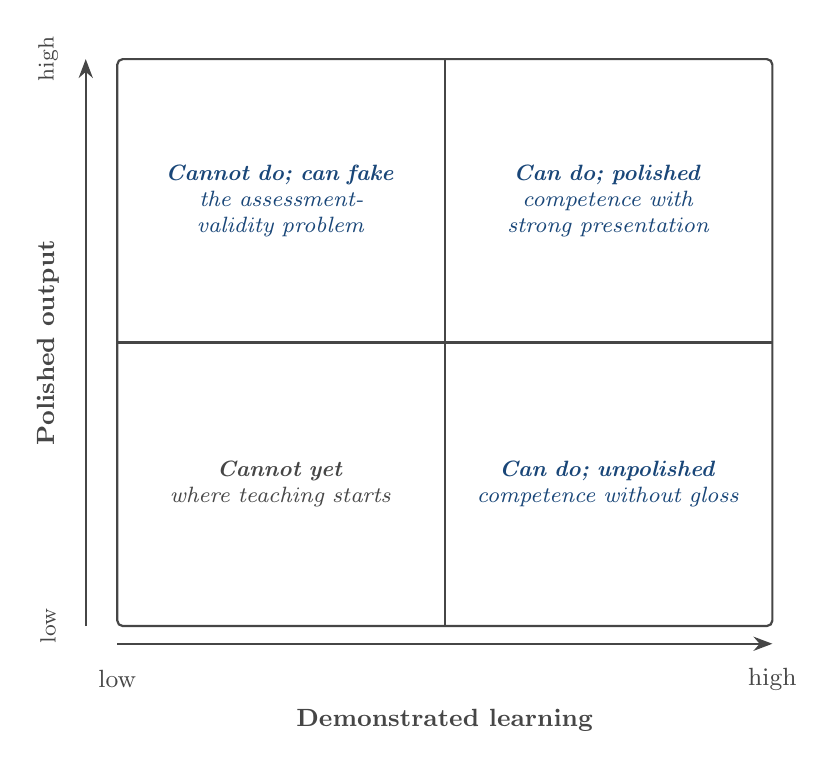
\begin{tikzpicture}[x=1.6cm, y=1.5cm]
% Quadrant boundaries
\draw[thick, draw=darkgray] (-2.6, 0) -- (2.6, 0);
\draw[thick, draw=darkgray] (0, -2.4) -- (0, 2.4);

% Outer frame
\draw[thick, draw=darkgray, rounded corners=2pt] (-2.6, -2.4) rectangle (2.6, 2.4);

% Quadrant labels
\node[quadrant-label, color=guideblue] at (-1.3, 1.2) {\textbf{Cannot do; can fake}\\\footnotesize the assessment-validity problem};
\node[quadrant-label, color=guideblue] at (1.3, 1.2) {\textbf{Can do; polished}\\\footnotesize competence with strong presentation};
\node[quadrant-label, color=darkgray] at (-1.3, -1.2) {\textbf{Cannot yet}\\\footnotesize where teaching starts};
\node[quadrant-label, color=guideblue] at (1.3, -1.2) {\textbf{Can do; unpolished}\\\footnotesize competence without gloss};

% Axis labels
\node[axis-label] at (0, -3.2) {\textbf{Demonstrated learning}};
\node[axis-label] at (-2.6, -2.85) {low};
\node[axis-label] at (2.6, -2.85) {high};
\node[axis-label, rotate=90] at (-3.15, 0) {\textbf{Polished output}};
\node[axis-label] at (-3.15, 2.4) {\rotatebox{90}{\footnotesize high}};
\node[axis-label] at (-3.15, -2.4) {\rotatebox{90}{\footnotesize low}};

% Axis arrows
\draw[flow-arrow] (-2.6, -2.55) -- (2.6, -2.55);
\draw[flow-arrow] (-2.85, -2.4) -- (-2.85, 2.4);
\end{tikzpicture}
\caption{\textbf{Polished output vs.\ demonstrated learning.} Final polish and underlying competence are independent. The upper-left quadrant is the assessment-validity problem: high polish without learning. Strong AI-aware course design moves student work toward the right two quadrants and gives instructors evidence to distinguish all four cases. Tool use can land anywhere on this grid, with or without AI; that is why the axes are polish and learning rather than tool and no-tool.}
\label{fig:polished-vs-learning}
\end{figure}

Survey evidence from 2026 supports the same reading. Assessments become weaker indicators of capability when they judge polished final work without evidence of process, judgment, and independent performance. The authors conclude that the remedy is assessment reform rather than bans and detection \citep{chirikov2026generative}.

One caution belongs here. Controlled conditions are the most direct way to see independent work, and a reader of this Part could conclude that more of them is always better. It is not. An exam written without help gives a clean read on Core Competence. It says almost nothing about whether that student can scope a project, weigh a source, or work with a tool honestly. Assessment research makes this point against assignments built mainly to defeat AI, which rarely capture the broader knowledge and judgment a program is trying to develop \citep{chirikov2026generative}. The framework here treats controlled work as one of three outcomes rather than the goal. Use it where independent competence is what you need to see, and carry the other two outcomes on assignments designed for them.

\subsection{Design features that weaken assessment validity}
\label{i:subsec:weak-features}

Some common assignment designs are now fragile.

\begin{itemize}
\item A take-home task graded only on final polish.
\item A generic prompt that can be answered well by a public chatbot.
\item A writing assignment with no draft history or author reflection.
\item A coding assignment graded only on whether it runs.
\item A problem set where students submit only final answers.
\item A citation-heavy assignment with no source verification requirement.
\end{itemize}

These assignments may still be useful for practice, but they should not carry too much weight as evidence of independent understanding.

\subsection{Skill: when doing is the evidence}
\label{i:subsec:skill}

The diagnostics in this Part, and the three models that follow, mostly test what a student can explain. The translation test asks a student to say a thing in another form; an oral defense asks a student to account for the work. These are the right checks for understanding that lives in words and symbols.

Some competence does not. A student who can run the assay, suture the wound, throw the pot, or execute the design owns that work whether or not they narrate it well. For skill of this kind the evidence is the performance, not the account of it. A practiced welder may struggle to put the motion into sentences and still lay a flawless bead. Grading the explanation would measure the wrong thing, and demanding one can understate what the student has.

The design response is to assess skill by having the student do it under observation, with the same care for ownership the rest of this Part asks for. Watch the technique, vary the conditions, ask for a repair or a next step, and judge the doing. AI's role shifts to match. For skill it is a coach rather than a source to verify: where the domain allows, it can give feedback on form, generate graded practice, or run simulations to rehearse against. There is no claim to check, only a performance to build. Any of the three models can carry this; what changes is not the model but what counts as the evidence. For a skill, it is the work performed, not the work described.

\begin{table}[ht]
\centering
\caption{\textbf{Three assessment models compared.} The Oral-Defense Model relies on live questioning to confirm understanding; the Evidence-of-Thinking Model relies on process artifacts that are difficult to outsource; the Hybrid Model combines both. The right model is the one that fits the course size, staffing, and goals.}
\label{tab:three-models}
\small
\begin{tabularx}{\textwidth}{>{\raggedright\arraybackslash}p{2.0cm} >{\raggedright\arraybackslash}X >{\raggedright\arraybackslash}X >{\raggedright\arraybackslash}X}
\toprule
 & \textbf{Oral-Defense} & \textbf{Evidence-of-Thinking} & \textbf{Hybrid} \\
\midrule
\textbf{Best for} & Small classes; seminars and honors courses; graduate courses & Large lectures; service courses; online courses & Medium courses; lab and project work; multi-TA staffing \\
\addlinespace
\textbf{Evidence sources} & Oral conferences; live questioning; submitted work; in-class observation & Process artifacts; in-class quizzes; random audits; submitted work & Mix of oral and process; spot oral checks; process artifacts; in-class checks \\
\bottomrule
\end{tabularx}
\end{table}

These models are operationally plausible, and direct evidence shows the Hybrid pattern can work in at least one setting. A programming course for novice programmers was redesigned along these lines: home assignments an AI chatbot could not complete directly, lab time spent on oral defenses of submitted code, and a paper-and-pencil midterm focused on concepts. Students with and without AI access reached similar learning outcomes \citep{kosar2024computer}. That redesign is closest to the Hybrid Model, and \cref{i:subsec:hybrid-anchors} gives the detail. The same design logic underlies all three models: what students learn depends on the assessment design, not on whether they used AI. The Oral-Defense and Evidence-of-Thinking models await their own direct evidence.

\section{AI tools for teaching preparation}
\label{i:sec:prep-capabilities}

AI can now help with much of the work of preparing to teach, and an instructor cannot adopt a capability
they have not seen. The durable point is short, and the practical detail belongs elsewhere. What follows
names the kinds of help that exist; the companion repository maintains the working guide to them.

These uses share a low risk profile because they act on your own materials, not on student assessment.
The same tools can rewrite a passage at several reading levels for a mixed class, turn an outline into
draft slides or a worked-example set, propose quiz questions or a first-pass rubric from your content,
convert a reading into audio or a figure into a described alternative for accessibility, draft routine
communication, or turn a recorded lecture into notes for a student who missed it. The higher-risk uses,
AI feedback on student work and AI-assisted grading, are different in kind and are treated with their
boundaries in \cref{i:sec:instructor-ai-use}.

Every one of these produces a draft, and the instructor who uses it is responsible for checking the
result. That is the whole of what this book needs to say. AI removes the friction of a first draft. It
does not remove the responsibility to verify, and it does not replace the judgment that made you the
teacher of the course.

The rest is practical, tool-specific, and changes too fast for print. The companion repository keeps a
working guide to teaching-preparation tools: what each kind of tool is good for, how to use it well, what
a good result looks like, and how to obtain current tools, most of which have free versions
(\texttt{companion/instructor-capabilities/}). It is meant to be updated as the tools change, which they
will.

\chapter{Assessment Models}
\label{i:ch:assessment-models}%

\bookepigraph{A mistake is not yet a lesson.\\The lesson begins when you ask why.}

\index{automation bias}Automation bias is documented outside education. In one study, people ran a monitoring task with and without a reliable automated aid. The ones without the aid did better. The ones with it missed problems the aid did not report, and followed its recommendation even when their training and every other reliable indicator said otherwise \citep{skitka1999does}. The aid was accurate almost all the time. Almost was enough.

The mechanism is substitution. A person watching a system attends to many things at once and names none of them. Hand that watching to a tool and the many collapse into the few the tool reports. The tool does less than the person was doing, and the person credits it with the whole job. Grading works this way too. Reading a student's work, you register whether the reasoning holds, whether the writing is understood or copied, whether the explanation would survive one follow-up question. Replace that reading with a proxy, a rubric line, a detector score, an automated grade, and your attention narrows to what the proxy reports. Work passes while the learning is absent, and the gap does not announce itself, because the proxy gave an answer and answers feel like knowledge.

What makes this usable is that the bias responds to arrangement. People told they would answer for their accuracy checked more \citep{skitka2000accountability}. Engineering students who met the automation failing during training went on to check its recommendations more carefully than those who were only told it could fail, though the training did not stop the errors it made less likely \citep{bahner2008misuse}. The bias is not fixed. It responds to how the work is set up. The three models that follow are ways of setting it up.

\section{Where this fits in a grade you already give}
\label{i:sec:grade-formula}%
\index{grade weighting}\index{grade weighting!splitting a component}\index{syllabus!grade formula}

Every course already divides its grade. Homework, exams, attendance, a final, sometimes writing. The models in this chapter do not replace that formula. They divide some of its lines.

A calculus course grades homework at 20 percent, two midterms at 30, a final at 40, and attendance at 10. To run the Evidence-of-Thinking Model, split the homework. Ten percent stays no-AI work done and checked in class. Ten percent becomes AI-assisted work submitted with a short verification note. The midterms, the final, and attendance do not move. The formula still sums to 100 and the registrar never hears about it.

This matters more than it looks. Nothing here needs a new record, a new transcript line, a committee, or anyone's approval above the instructor. Weighting is already the instructor's to set. A department can adopt every idea in this book without asking its institution for anything.

The cost is that one number carries both things. A student who is strong alone and careless with AI, and a student who is the reverse, can finish the term with the same grade, and nobody reading it later can tell them apart. Inside a course that is usually fine, because the instructor saw both halves. It matters more the further the grade travels. Appendix~\ref{app:gmip} develops the alternative and names what it costs.

That balance may not hold. If employers or graduate programs begin asking what a student can do without assistance, a single blended grade will stop answering the question, and separating the record will become worth its price. The approach in this chapter is the right one now. It is not obviously the right one permanently.

\section{The Oral-Defense Model}
\label{i:sec:oral-defense-model}%
\index{Oral-Defense Model}

The Oral-Defense Model is best suited to small classes of any level: seminars, honors courses, writing workshops, independent studies, capstones, advanced labs, and many graduate courses. The model is class-size-driven; it works wherever the instructor (or trained TAs) can speak directly with each student about their submitted work. The assignment-category mix and the AI autonomy granted to students will shift with course level (\cref{i:subsec:category-by-level}), but the assessment model itself is the same. \Cref{tab:three-models} compares the three assessment models in this Part. \Cref{i:app:oral-rubric} gives a rubric for the defense itself.

The model rests on a simple principle:

\begin{quote}
\textbf{Students may use AI more extensively when they can personally defend the work.}
\end{quote}

An oral defense does not need to be adversarial. It can be a teaching conversation. Its purpose is to test whether the student's submitted work has become part of the student's understanding.

\subsection{Recommended structure}
\label{i:subsec:oral-structure}%
\index{oral examination}

A short oral defense can take 15 to 20 minutes. A fuller version can take 30 to 60 minutes. The following structure works across disciplines.

\begin{center}
\begin{tabular}{p{0.18\textwidth}p{0.75\textwidth}}
\toprule
\textbf{Segment} & \textbf{Purpose} \\
\midrule
Student summary & The student explains the submitted work in their own words. \\
Core question & The instructor probes a central concept, method, source, or decision. \\
Audit-and-repair & The student critiques a flawed AI response or a flawed piece of their own process. \\
Transfer question & The student applies the idea to a new but nearby situation. \\
Process defense & The student explains how AI was used, checked, and limited. \\
\bottomrule
\end{tabular}
\end{center}

Where more than one person runs these defenses, the teaching team should agree on what a strong answer looks like for each segment before the first one. See \cref{i:sec:ta-calibration}.\index{TA calibration!for oral defense}\index{second reader}

\subsection{Examples across fields}
\label{i:subsec:oral-examples}

In mathematics, the student may prove a result at the board, identify which hypotheses matter, and repair a flawed proof. In biology, the student may explain the design of an experiment and interpret a surprising result. In history, the student may defend the use of a primary source and distinguish evidence from background summary. In writing, the student may explain why a paragraph was revised and how the claim changed. In computer science, the student may walk through code and predict what happens on an edge case.

The format changes by discipline. The purpose remains the same: the student must show ownership.

\subsection{Equity in oral assessment}
\label{i:subsec:oral-equity}%
\index{equity and access!in oral assessment}

Some students hear ``oral audit'' as threatening, even when the instructor intends a teaching conversation. A few small adjustments protect fairness without weakening the assessment. Share sample audit questions in advance so students can prepare. Grade for understanding, not verbal polish. Allow students to point to their work, write a formula, sketch a diagram, or explain in steps; oral does not have to mean spoken-only. The goal is ownership, not performance under pressure. These adjustments help multilingual students, shy students, neurodivergent students, and students who understand the material but need a moment to organize their explanation. The Oral-Defense Model is a calibration-restoring design; the calibration is of student understanding, not of presentation skill.

Two further considerations matter. First, students with documented accommodations through the institution's disability services (including students with anxiety disorders, students who use augmentative communication, students who are deaf or hard of hearing) may need formats beyond the spoken-aloud audit. A short written explanation, a signed conversation, a typed exchange, or a recorded video with subtitles can satisfy the diagnostic purpose while accommodating the student. The framework is about ownership of work, not about fluency in any particular mode of demonstration. Second, instructors who can do so should make alternative formats available to any student on request, not only those with formal accommodations on file. Some students whose understanding is sound will struggle in live questioning for reasons that do not appear on any accommodation letter; quiet flexibility about format protects the model's validity.

\subsection{Worked example: a small seminar}
\label{i:subsec:oral-worked-example}

A 14-student upper-division seminar meets once a week. Each student gives one oral defense during the term, fifteen minutes, scheduled in office hours, on a paper they choose. The defense follows the five segments above. The student summarizes the work, answers one core question, repairs a flawed passage the instructor supplies, takes one transfer question, and explains how AI was used and checked. The grade rests on ownership, not on verbal polish, and the instructor shares sample questions in advance so the conversation is preparation rather than ambush. A student who used AI heavily and a student who used none can both earn full marks, because the defense, not the AI policy, sets the grade.

\subsection{Suggested weighting for small classes}
\label{i:subsec:small-weighting}

\begin{center}
\begin{tabular}{p{0.75\textwidth}>{\raggedleft\arraybackslash}p{0.18\textwidth}}
\toprule
\textbf{Component} & \textbf{Typical weight} \\
\midrule
Core competence assessments & 30--40\% \\
AI-integrated assignments or projects & 25--35\% \\
Oral defense or conference & 20--30\% \\
Disclosure, verification, and reflection & 10--15\% \\
\bottomrule
\end{tabular}
\end{center}

These weights are only a starting point. A writing workshop may place more weight on conferences and revision. A lab course may emphasize practical demonstration. A proof-based course may require a higher independent competence threshold.

\section{The Evidence-of-Thinking Model}
\label{i:sec:evidence-model}%
\index{Evidence-of-Thinking Model}\index{process evidence}

The Evidence-of-Thinking Model is designed for large classes where one-on-one oral defense is not feasible for every student: large lectures, service courses, multi-section courses, general education courses, and online courses. Most large classes happen to be undergraduate simply because that is where enrollment concentrates, but the model is class-size-driven, not level-driven. A large advanced course or a large graduate-equivalent course uses the same evidence-of-thinking patterns, with the assignment-category mix shifting with course level (\cref{i:subsec:category-by-level}).

The model rests on a different principle:

\begin{quote}
\textbf{When individual oral examination is not feasible, the course should collect repeated, low-cost evidence of student thinking.}
\end{quote}

This model does not assume dishonesty. It assumes that polished products are no longer enough. In a large course, instructors need scalable ways to see whether students understand what they submit.

\subsection{Recommended structure}
\label{i:subsec:evidence-structure}

A course using this model does not need every component that follows. A workable default combines three: a stream of low-cost process artifacts on regular assignments, a small set of in-class checks that cannot be outsourced, and sampled audits that make the process artifacts worth taking seriously. The weighting and staffing then scale with enrollment.

\begin{center}
\begin{tabular}{p{0.24\textwidth}p{0.69\textwidth}}
\toprule
\textbf{Component} & \textbf{Purpose} \\
\midrule
Process artifacts & Plan-Use-Verify notes or draft histories on regular assignments make thinking visible at scale. \\
In-class checks & Short no-AI writing or problem solving anchors the grade to work done under observation. \\
Sampled audits & Random oral or written audits on a fraction of submissions create probabilistic accountability. \\
Weighting and staffing & The component mix and the grading load scale with enrollment. \\
\bottomrule
\end{tabular}
\end{center}

\subsection{Scalable evidence sources}
\label{i:subsec:scalable-evidence}%
\index{process log}

Useful evidence sources include short no-AI quizzes, homework-to-quiz transfer questions, in-class writing, process logs, source-verification sheets, draft histories, lab notebooks, code test reports, AI-output critiques, video explanations, peer review, and random oral audits.

The goal is to distribute accountability across the term. A course with ten small checks is often more robust than a course with two high-stakes take-home assignments.

Process evidence should be short and targeted. Long AI transcripts and lengthy prompt logs should not be rewarded for length, since process documentation can drift into theater. The useful evidence is a decision, a verification step, a correction, or a change in understanding. Evidence-of-Thinking is not a paperwork model; it is a calibration model that reads small artifacts for signal.

\subsection{Worked example: a large lecture}
\label{i:subsec:evidence-worked-example}

A 280-student introductory lecture cannot defend every student orally, so it leans on repeated low-cost evidence. Every weekly problem set carries a three-line Plan-Use-Verify note. Each Friday section opens with a five-minute no-AI transfer quiz on the prior week. Teaching assistants read a random tenth of the Plan-Use-Verify notes closely each week, and any submission that crosses a stated complexity threshold draws a short written audit. No single check carries much weight. Together they let a polished-hollow submission stand out against the student's own quiz scores and process record, without the instructor reading every prompt from every student.

The cost of this is bounded, but it is not zero, and it is worth being concrete about both. Reading a random tenth of the notes and running one short quiz per section adds a few hours per assignment cycle, not the dozens that reading every prompt would take. The labor it does require is recurring and intellectual: writing transfer questions that probe the week's idea rather than its surface, calibrating what an audit should look for, and keeping rubrics current. Teaching assistants can carry much of the sampling, but only if they are trained to grade for the presence of a genuine process rather than its depth: did the student plan, use AI, and verify the result? A course that asks a teaching assistant to judge the depth of thirty such notes each week breaks. A course that asks whether each was genuinely attempted scales.

\subsection{Suggested weighting for large classes}
\label{i:subsec:large-weighting}

\begin{center}
\begin{tabular}{p{0.75\textwidth}>{\raggedleft\arraybackslash}p{0.18\textwidth}}
\toprule
\textbf{Component} & \textbf{Typical weight} \\
\midrule
Short no-AI checks & 25--35\% \\
AI-assisted homework or projects & 20--30\% \\
Process evidence and verification notes & 15--20\% \\
AI critique or error-detection tasks & 10--20\% \\
Random oral, video, or TA-led checks & 5--10\% \\
Reflection and disclosure & 5--10\% \\
\bottomrule
\end{tabular}
\end{center}

A large course does not need to use every component. The important point is balance. Students should have chances to practice with AI, but the course should also include direct evidence of independent understanding.

\subsection{Random oral audits}
\label{i:subsec:random-audits}%
\index{random audit}

A random oral audit is a short conversation about submitted work. It may last five to eight minutes. Students know in advance that any AI-assisted assignment may be selected. \Cref{i:app:audit-script} gives a script for the conversation.

A good audit asks ordinary questions.

\begin{itemize}
\item Explain the main idea of your submission.
\item What did AI help with?
\item What did you change after checking the output?
\item Show me one place where you verified a claim.
\item What would change if this assumption were different?
\end{itemize}

The audit should be framed as part of the course design, not as an accusation. It protects fairness by holding everyone to the same expectation: if students submit work, they should understand it.

\subsection{TA-supported mini-conferences}
\label{i:subsec:ta-mini-conferences}%
\index{TA calibration}

In multi-section courses, trained teaching assistants can conduct short structured conferences. The instructor should provide a common script and rubric. TAs should grade a small sample together before conducting conferences independently.

This structure is most useful when assignments are AIC or AIS. It helps ensure that AI-assisted work remains connected to student understanding.

\subsection{The seeded-error check}
\label{i:subsec:seeded-error-check}%
\index{seeded-error check}\index{verification!measuring}

Verification is easy to assert and hard to measure. This check measures it.

Take a piece of AI-produced work in your subject and plant a fixed number of errors in it. Vary them: one that any careful reader catches, one that requires knowing the material, one that requires checking a source. Give students the passage, tell them how many errors it contains, and ask them to find and explain each one.

Scoring is the detection rate. A student who finds four of five has demonstrated something a polished submission cannot demonstrate. A class that averages one of five has told you where the term needs to go.

Three things make it work. Tell students the count, so the task is detection rather than suspicion. Ask for the explanation, not the flag, because naming why something is wrong is the competence being measured. And change the errors between terms.

It scales. The passage is written once, the errors are known in advance, and scoring is mechanical enough to delegate. Difficulty is set by how subtle the planted errors are, which makes the same check usable in a first-year course and a graduate seminar. The chapter opened with the finding that people who met the automation failing checked its later advice more carefully. This is that experience, arranged as coursework.

\section{The Hybrid Model}
\label{i:sec:hybrid-model}%
\index{Hybrid Model}

Many courses fall between the small-class and large-class models. A class may be too large for full oral exams but small enough for some direct contact. A lab course may have many students but strong TA support. A writing course may have conferences for major projects but not for every assignment. The Hybrid Model is the realistic choice for most courses; it is the third of the three calibration-restoring designs presented in this Part. Process artifacts carry most of the load, while sampled live conversation provides direct verification at the rate the staffing allows.

Useful hybrid tools include group oral exams, sampled oral audits, short student conferences, video explanations, peer review with instructor spot-checking, TA-led recitations, and in-class transfer questions. The pattern is to use live explanation where it matters most and process evidence everywhere else. The remainder of this section develops the model with the same four-element treatment used for the Oral-Defense and Evidence-of-Thinking models: recommended structure, sampling strategy for live elements, a worked example, and suggested weighting.

Peer critique deserves more than its place in that list. Asking a student to review another student's work tests something the artifact cannot. To judge an argument, a reviewer has to understand the subject, decide whether the evidence supports the claim, locate the weak points, and say how the work could be improved. A student who cannot do the work usually cannot review it well either, and the review leaves a record of the attempt.

This resists AI for a different reason than the other designs here. It does not remove the tool or try to detect it. It makes the evidence relational, since two students are each accountable for reading the other. The obvious objection holds, because a review can be AI-generated like anything else. The answer is the same as everywhere else in this Part. Grade the review as work, ask the reviewer to defend a judgment in person, and spot-check.

Grading any live or process element carries one more obligation. A rubric line for reasoning visibility assumes students know how to show reasoning, and most have never been asked to do it in front of anyone. The rule this guide applies to disclosure applies here as well: treat a weak first presentation as missing instruction rather than missing ability. Model one before grading any. Show the tool's output beside what a group did to it, and name what made the checking good.

\subsection{Recommended structure}
\label{i:subsec:hybrid-structure}

A hybrid course pairs one or more live elements with continuous process evidence. The pairing depends on the staffing and the course type. \Cref{tab:hybrid-mapping} sketches the mapping for four common course types.

\begin{table}[ht]
\centering
\caption{\textbf{Hybrid pairings by course type.} The live element provides direct verification of understanding; the process element distributes accountability across the term.}
\label{tab:hybrid-mapping}
\begin{tabularx}{\textwidth}{>{\raggedright\arraybackslash}X >{\raggedright\arraybackslash}X >{\raggedright\arraybackslash}X}
\toprule
\textbf{Course type} & \textbf{Live element} & \textbf{Process element} \\
\midrule
Lab course (intermediate enrollment, strong TA support) & Lab-time oral defense of submitted code or analysis & Lab notebook, code tests, in-class transfer questions \\
\addlinespace
Medium lecture (40--80) with TAs & Sampled TA-led conferences once per term per student & Process logs, weekly transfer quizzes \\
\addlinespace
Writing course with conferences (20--40) & Mid-term and final 20-minute conferences on major projects & Draft histories, author's notes, in-class writing \\
\addlinespace
Flipped-classroom STEM (any size) & In-class problem-solving with instructor circulation & AI-tutor logs from pre-class material, post-class transfer quizzes \\
\bottomrule
\end{tabularx}
\end{table}

The mapping is illustrative; many other pairings work. The instructor's task is to identify the live element the staffing supports, then design process evidence to cover the rest of the term. A common error is to over-design both elements, producing a course that asks students to document everything and defend everything, which collapses into paperwork. The hybrid model works when each element does its part: the live element verifies depth on a sampled basis; the process element provides continuous low-cost evidence.

\subsection{Sampling strategy for live audits}
\label{i:subsec:hybrid-sampling}%
\index{sampling!live audits}

When a course cannot conference every student on every assignment, the instructor must choose how to sample. Three sampling strategies are common, with different trade-offs.

\emph{Random sampling.} Every student has the same probability of being audited on every assignment. Fairest in expectation, simplest to administer, hardest to argue with. Works well when the course has enough audits per term that most students will be sampled at least once. The drawback is statistical: a student with weak understanding may not be sampled on the assignment where the gap is largest.

\emph{Stratified sampling.} The instructor stratifies the population (by submission quality, by stated AI use, by prior audit history, or by self-selection through optional sign-up) and samples within strata. Concentrates effort where it adds most assessment information. The risk is the appearance of targeting; the strata should be public and the rationale should be educational rather than punitive.

\emph{Threshold sampling.} The instructor audits any submission that meets a threshold condition (a confident-sounding answer to a problem the student has not worked on in class; a major project crossing a stated complexity boundary; a flagged inconsistency between submitted work and prior work). Most efficient when the thresholds are known in advance. Vulnerable to adverse-selection effects: students who learn the thresholds may submit work that just stays under them.

A hybrid course can mix strategies across the term. For example, a course might use random audits early, when the threshold for problematic submissions is still being calibrated. It might use stratified or threshold audits later, when the instructor has seen enough of each student's work to recognize patterns.

\subsection{Worked example: a hybrid course across the semester}
\label{i:subsec:hybrid-example}

Consider a 60-student intermediate course with two TAs. Class meets twice weekly for 75 minutes; one TA-led recitation per week. The instructor designs the course as follows.

\emph{Week 1.} Students complete the AI account configuration template (\cref{app:ai-config}) as a no-credit first assignment. The instructor explains the course's category mix (mostly AIT and AIC; one NAI mid-term; one AIS critique exercise late in the term).

\emph{Weeks 2--4.} AIT and AIC homework assignments, each requiring a short Plan-Use-Verify artifact (one short paragraph each for plan, use, and verify). Weekly 5-minute in-class no-AI transfer quizzes on the prior week's material.

\emph{Week 5.} Each student completes a 5-minute calibration conference with their assigned TA. The conversation is structured: the student summarizes one recent assignment, answers one transfer question, and describes their AI use pattern. The TA records a brief note. This early conference is for calibration, not grading.

\emph{Weeks 6--9.} Continued homework + transfer quizzes. One AIS-category critique assignment around Week 8 (students critique an AI-generated answer to a course-relevant problem and identify two errors). Process logs are required for every assignment; the instructor reads only the verification notes, sampling the rest.

\emph{Week 10.} Mid-term exam: paper-and-pencil, no-AI, weighted as the NAI component of the course.

\emph{Weeks 11--14.} Larger AIC-category project. Students submit a project proposal at Week 11; receive AI-assisted draft feedback at Week 13; submit a final draft at Week 15. Each student's project culminates in a 10-minute oral defense during the final week.

\emph{Week 15.} Project oral defenses (in-class, with the instructor present and TAs as second readers).

\emph{Final.} Cumulative process review. The instructor scores process artifacts across the term, weighted as a single component.

The course distributes assessment across the term: weekly small no-AI checks, two oral conferences (early calibration + final defense), one paper-and-pencil mid-term, one AIS critique, one Plan-Use-Verify pattern on every AIC assignment. No single assessment carries excessive weight; no single modality is the only path to demonstrating learning.

\subsection{Suggested weighting for hybrid classes}
\label{i:subsec:hybrid-weighting}

\begin{center}
\begin{tabular}{p{0.75\textwidth}>{\raggedleft\arraybackslash}p{0.18\textwidth}}
\toprule
\textbf{Component} & \textbf{Typical weight} \\
\midrule
Core competence assessments (no-AI quizzes, mid-term, NAI components) & 25--35\% \\
AI-integrated assignments or projects (AIC) & 25--35\% \\
Process evidence and verification notes (Plan-Use-Verify artifacts) & 15--20\% \\
Sampled oral, video, or conference checks & 10--15\% \\
AI critique tasks (AIS) & 5--10\% \\
Reflection and disclosure & 5--10\% \\
\bottomrule
\end{tabular}
\end{center}

These weights are starting points. A lab course will weight the live lab-time defense higher; a writing workshop will weight conferences and revision higher; a foundational course will weight no-AI assessments higher. The principle is that no single modality should carry the whole assessment load. The models are also a destination rather than an entry point, and \cref{i:sec:workflow} gives the three moves an instructor can make first, without choosing a model at all. A student who is weak on one modality but strong on others should be visible to the instructor as the intermediate case they are, not as a failing student.

\subsection{Two empirical anchors}
\label{i:subsec:hybrid-anchors}

Two recent studies provide empirical grounding for the patterns above. \citet{kestin2025ai} showed in their RCT that an AI tutor designed around the seven pedagogical practices listed in \cref{i:sec:assignment-design} could outperform in-class active learning on the introductory material it covered, when measured by post-test learning gains. The implication for course design is not that AI should replace classroom instruction. The implication is that, when AI tutoring is well-designed, it can effectively bring all students up to a level where in-person class time can be spent on advanced problem solving, project work, group discussion, and the kinds of higher-order tasks that benefit most from a faculty member's presence. Used this way, AI tutoring functions as a flipped-classroom mechanism, with the AI handling first exposure and the instructor handling deepening, transfer, and oral assessment.

\citet{kosar2024computer} report a more direct precedent for the Oral-Defense and Evidence-of-Thinking elements that hybrid courses combine. They redesigned a programming course for novice programmers by changing home assignments so they could not be directly completed by an AI chatbot, using lab time for oral defenses of submitted code with ``understanding'' questions, and converting the mid-term exam to paper and pencil with a focus on conceptual understanding. The redesign produced similar learning outcomes for student groups with and without GenAI access. The redesign described in that study is operationally close to the hybrid pattern recommended here. Their finding, that the with-AI and without-AI cohorts converged when the assessment design carried the load, is the closest direct precedent available for the Hybrid pattern. It supports the plausibility of the broader design logic, but the Oral-Defense and Evidence-of-Thinking models await direct evaluation of their own.

\section{Group and collaborative assignments}
\label{i:sec:group-assignments}%
\index{group assignments}

Group and project work adds an assessment problem that AI sharpens. A shared product is even weaker evidence of any one student's competence than an individual submission, because the contributions of several students and of AI are combined in a single artifact. The three assessment models extend to this case rather than being replaced by it. Under the Oral-Defense Model, ask each member to defend the part they contributed, not only the group to present the whole. Under the Evidence-of-Thinking Model, require individual-contribution artifacts, so that each student's process is visible alongside the joint result. The Hybrid Model combines the two and is often the right choice for project courses.

Two design choices do most of the work. First, ask the group to agree on and state its AI-use norms, in the same way an individual assignment states its category (\cref{i:sec:assignment-categories}). A team that has not discussed whether AI may draft its shared text will discover the disagreement at the worst time. Second, collect evidence of each member's individual contribution, so that the grade reflects what each student learned rather than the polish of the combined output. A short individual reflection or a brief oral check per member is usually enough.

The two senses of collaboration are worth keeping distinct. AI as a collaborator is the \AIC{} category; collaboration among students is the peer interaction that good group work is meant to build. The two can pull against each other. A team that quietly divides the work and routes each piece through AI has neither collaborated with one another nor learned much, which is the erosion of peer learning noted in \cref{i:sec:assignment-design}. Group assignments are stronger when they reward genuine joint reasoning and weaker when they reduce to parallel individual work stapled together. The strongest group work also rewards disagreement. A team whose members challenge one another's reasoning, rather than dividing the task and trusting each piece, practices the same scrutiny they must apply to AI. An assignment that asks a group to surface and resolve its disagreements, not only to produce a joint answer, builds that habit. The student-facing counterpart to this section is \cref{sec:group-assignments}.

\section{Feedback and grading with AI}
\label{i:sec:instructor-ai-use}%
\index{feedback and grading with AI}

Instructors may also use AI. This can be legitimate and useful, but it requires boundaries.

Feedback design is one of the most-studied levers in the learning-science literature, building on the foundational case for formative assessment made by \citet{black1998assessment}. Effective feedback addresses three questions for the learner: where am I going, how am I going, and where to next; and it works best when directed at task and process rather than at the person \citep{hattie2007power}.

AI may help instructors draft practice questions, generate examples, identify possible misconceptions, rewrite assignment instructions, produce alternate explanations, create low-stakes quizzes, and draft preliminary feedback. These uses can save time and improve student support. The standards that govern this work are the ones in Appendix~\ref{app:sciwriting}: an instructor who drafts a problem with AI verifies it, and discloses the assistance where a reader would want to know. Writing a fresh problem set beats reissuing one from six years ago, and the verification is what makes it safe to do.

But final evaluative judgment remains the instructor's responsibility. AI should not assign final grades. It should not decide whether misconduct occurred. It should not be used in ways that violate student privacy or institutional data rules.

A good instructor-facing standard mirrors the student standard:

\begin{quote}
\textbf{AI may assist judgment, but it must not replace or inhibit it.}
\end{quote}

\subsection{Safe uses of AI for feedback}
\label{i:subsec:safe-feedback}

Relatively safe uses include asking AI to suggest clearer wording for feedback already written by the instructor, generate additional practice questions for common errors, produce alternative explanations of a concept, or check whether a rubric covers the intended learning outcomes.

Even here, the instructor should review the output. AI-generated feedback can sound confident while missing the actual student difficulty. It can also become too generic to help.

When using AI to draft feedback on student errors, prompt the AI for scaffolded hints rather than complete corrections. An instructor who uses AI to fully rewrite a student's flawed paragraph and hands it back has simply outsourced the cognitive offloading; the desirable difficulty \citep{bjork2011making} that produces learning is lost. Hints, leading questions, or partial models preserve the work the student still needs to do, which is the work that produces the learning. Tell students when AI helped make what they receive. The standard is the one you are asking of them: what tool, how it was used, what it contributed, what you changed, and how you checked it. A line in the syllabus covers standing practice. A sentence on the work itself covers the times it matters, as when AI drafted the comments on their paper. The point is not confession. It is the same record of process the students are keeping.

A constructive recent example is the \emph{Tutor CoPilot} system developed at Stanford, an AI tool finetuned on ethnographic observations of effective tutoring and integrated into an online tutoring platform. In a randomized study with 900 tutors working with 1,800 underserved students in the United States, the tool raised student pass rates by an average of 4 percentage points, with the largest gains (7 to 9 percentage points) for less-effective tutors and smaller gains for stronger ones \citep{wang2024tutor}. The study is currently circulating as an Annenberg working paper pending journal publication, and the specific effect sizes should be read with that status in mind. The pattern is informative even at preliminary status: AI assistance supporting human teachers produced measurable benefits without replacing the human teaching role. For instructors thinking about how AI might support their own feedback workflow, this study illustrates that the most useful design point is often AI that scaffolds the less-experienced rather than AI that replaces the experienced.

\subsection{High-risk uses of AI for grading}
\label{i:subsec:risky-grading}

High-risk uses include uploading identifiable student work to unapproved tools, using AI to assign scores without human review, using AI-generated accusations of misconduct, or using a model's explanation as the sole basis for a grade.

These practices can harm students and weaken trust. They should not be adopted without explicit institutional approval, privacy review, and human oversight.

\chapter{Integrity, Equity, and Discipline}
\label{i:ch:integrity-equity-and-discipline}%

\section{Annotated dialogues: weak AI use as teaching cases}
\label{i:sec:dialogues-weak}

The following two dialogues show what weak AI use looks like and how an instructor might respond. They are paired with the strong-use dialogues in \cref{sec:dialogues-strong} so that an instructor can show students both versions side by side. Longer worked sessions, following one student through a messy problem turn by turn with the moves annotated, are in the companion repository (\texttt{students/study-sessions/}). They are useful to hand to a colleague who has never used one of these tools and wants to see what a student session actually looks like. The contrasts are pedagogically the most useful part: the boundary between strong and weak use is rarely about whether AI was used, and almost always about how the student engaged with the work.

\begin{dialogue}{Dialogue~7: Weak undergraduate use (calculus, contrast with Dialogue~1)}
\studentturn{Solve this calculus optimization problem: a farmer wants to fence a rectangular field of $400~\text{m}^2$ along a river, fencing only three sides. What dimensions minimize fencing cost?}
\dialogueannotate{Mistake: asked AI to solve, not for a hint.}

\aiturn{Let length parallel to river be $L$ and width be $W$. Constraint: $LW = 400$, so $L = 400/W$. Fencing cost is proportional to $f(W) = 400/W + 2W$. Setting $f'(W) = -400/W^2 + 2 = 0$ gives $W = \sqrt{200}$, so $L = 2\sqrt{200}$. Second derivative $f''(W) = 800/W^3 > 0$ confirms a minimum.}

\studentturn{Thanks. I'll submit this.}
\dialogueannotate{Mistake: did no independent work, no verification, no reconstruction.}

\studentturn{[At the random oral audit a week later.] Instructor: ``Why did you set up the function as $400/W + 2W$ rather than $L + 2W$?'' Student: ``I think because\dots\ I'm not sure. The AI did it that way.''}
\dialogueannotate{The audit reveals what the submission concealed: no understanding of the constraint substitution that is the key insight. Course rule violated: ``If you cannot explain it, it should not be in your work.''}

\studentturn{Instructor follow-up: ``What would change if the area constraint were $200~\text{m}^2$ instead of $400$?'' Student: ``I'd have to redo the problem with a new tool query.''}
\dialogueannotate{The student cannot transfer. This is the canonical failure mode the Learning Spiral (\cref{fig:learning-spiral}) is designed to prevent.}
\end{dialogue}

\noindent\textit{Instructor scoring}. This case illustrates the upper-left quadrant of \cref{fig:polished-vs-learning}: high polish, low demonstrated learning. A reasonable response under most course policies is partial credit on the submission (the answer is correct), zero credit on the oral audit, and a teaching conversation about how to use AI in this course. The same submission paired with the engagement shown in Dialogue~1 would receive full credit on both.

\begin{dialogue}{Dialogue~8: Weak graduate use (proof, contrast with Dialogue~2)}
\studentturn{Prove that every continuous function on $[0,1]$ attains its supremum.}
\dialogueannotate{Mistake: asked AI to produce the proof rather than to audit one.}

\aiturn{Let $M = \sup_{x \in [0,1]} f(x)$. Since $[0,1]$ is compact and $f$ is continuous, $f([0,1])$ is compact in $\mathbb{R}$, hence closed and bounded. Therefore $M$ is attained.}

\studentturn{Looks fine. I'll submit this.}
\dialogueannotate{Mistake: accepted a proof that uses a result (compactness implies attainment) that is essentially the conclusion. The AI proof is technically correct, but it bypasses the constructive Bolzano--Weierstrass argument the qualifying-exam syllabus expects.}

\studentturn{[Oral examination.] Examiner: ``Walk me through the step where you concluded $M$ is attained from compactness of $f([0,1])$.'' Student: ``A compact subset of $\mathbb{R}$ is closed and bounded, so the supremum is attained.''}

\studentturn{Examiner: ``Right. Now: prove that statement directly. Why is the supremum of a closed bounded subset of $\mathbb{R}$ attained?'' Student: ``\dots''}
\dialogueannotate{The student passed the surface but not the depth. GMIP D2 (proof construction \emph{and repair}; see Appendix~\ref{app:gmip}) requires producing the underlying argument when probed, not just citing the named theorem.}
\end{dialogue}

\noindent\textit{Instructor scoring}. The submission is correct mathematics. Under conventional grading it could pass. Under GMIP, the oral component reveals that the student has not built the underlying argument. Compare with Dialogue~2: the same student, given the same prompt, can engage with subtle critique, push back when AI is wrong, and produce a constructive proof. The framework distinguishes these two cases; the framework's job is to make that distinction visible.

\section{Academic integrity without detector dependence}
\label{i:sec:integrity}%
\index{academic integrity}\index{AI detectors}\index{AI detectors!false positives}\index{AI detectors!bias against non-native speakers}\index{AI detectors!perplexity-based detection}

AI detectors should not be the foundation of an academic integrity system. They produce both false positives and false negatives, and the magnitudes are not small. One study of seven widely used detectors quantified both failure directions; the figures, the perplexity mechanism that produces them, and the policy standard they support are laid out in Part~\ref{part:institutional} (\cref{u:sec:integrity}) \citep{liang2023gpt}. What matters in the classroom is the direction of the errors: the false positives concentrate on non-native writers, and the false negatives reward exactly the students most fluent at prompt refinement, so a detector score cannot carry an integrity decision alone.

The same mechanism reaches past language. Perplexity-based detection flags writing that departs from the model's expected norm, and non-native writers are not the only students whose writing departs from it. The same structural logic reaches autistic and other neurodivergent students, whose writing and reasoning a detector may also read as unusual. That extension follows from the mechanism rather than from a study that has tested it. The exposure is wider than text. Automated proctoring, engagement detection, and behavior analytics can misread a neurodivergent student's eye contact, pace, movement, or stress response as a sign of trouble, when it is only a different way of working. A system that judges people by how closely they match an assumed default penalizes whoever sits furthest from it. That is a fairness problem the institution owns, not the student.

The institutional consequences extend beyond accuracy. Detector-based enforcement creates what the same authors term a presumption of guilt: students are flagged as suspect by an automated system, and the burden falls on them to prove innocence. Even when an accusation is later revoked, the student's reputation and trust in the institution may not recover. The teaching-and-learning approach to academic integrity, developed long before AI tools were a concern, treats integrity as a pedagogical issue rather than a policing one \citep{bertramgallant2017academic}. The same orientation applies to AI-related concerns: when integrity is built into course design, fewer concerns arise, and those that do can be handled through evidence and conversation. When concerns arise, instructors should use multiple sources of evidence.

\begin{itemize}
\item Assignment policy and category.
\item Student disclosure or lack of disclosure.
\item Draft history or version record.
\item Source verification.
\item In-class performance.
\item Oral explanation or targeted reassessment.
\item Consistency with prior work, interpreted cautiously.
\item A fair conversation with the student.
\end{itemize}

The goal is not to avoid accountability. The goal is to make accountability fair, educational, and evidence-based.

Spot-checking does not require reviewing every student's AI conversation on every assignment. Reviewing three or four threads per assignment, chosen at random or based on signal, creates probabilistic deterrence at sustainable cost. Students who know that any single thread might be reviewed engage differently from students who know nothing is ever checked. The probabilistic version preserves the framework's three-cornered balance. The instructor's trustworthy-judgment corner is honored without making sustainability impossible, and the student-side disclosure practice in \cref{subsec:thread-sharing} becomes operationally useful for the instructor without requiring the workload of exhaustive review.

Faculty are not exempt from the integrity question\index{Northeastern case}. A senior at Northeastern University filed a formal complaint after she found her organizational behavior professor was using AI to produce his lecture materials, despite a syllabus that prohibited student AI use.\footnote{\citet{hill2025professors}; the case is discussed in full in Part~\ref{part:institutional} \cref{u:sec:problem}.} The asymmetry is the issue: an integrity rule that applies to students but not to those teaching them is structurally fragile, and students notice.

The framework developed in Part~\ref{part:student} for student AI use applies symmetrically to instructor AI use. The Instructor's Trilemma developed in \cref{i:sec:trilemma} names the three forces faculty navigate under AI pressure: professional sustainability, trustworthy professional judgment, and student learning. The Northeastern case can be read through that frame as a failure to hold trustworthy judgment together with the other two corners. The lecture materials presented to students implied a level of instructor engagement and expertise that the AI-assisted production did not actually back up; the syllabus claimed an integrity standard the instructor did not apply to himself.

The translation test gives both sides of the classroom a positive standard. A student who can translate their work into a different form is giving good evidence they own it; a student who cannot has reason to check further. A faculty member who can translate AI-assisted course material into their own language, with their own examples, in their own structure has integrated it. A faculty member who cannot has the analog of the polished hollow: course material the instructor cannot stand behind in conversation. The test is not punitive. It is a private check faculty can run on their own work before placing it in front of students, and a standard the institution can defend in public.

The translation test catches the \emph{polished hollow} mode of the Student's Trilemma (\cref{subsec:trilemma-failures}) directly, because the student cannot translate. The other two modes, \emph{strategic compliance} and \emph{honest risk}, require different instructor responses, developed in the rest of this Part. The parallel question for instructor misuse, what response sequence applies when faculty use AI without disclosure or in ways that contradict their own policies, is taken up in Part~\ref{part:institutional} \cref{u:sec:problem}.

\subsection{A fair response sequence}
\label{i:subsec:fair-response}

When AI misuse is suspected, a fair process can follow five steps.

\begin{enumerate}
\item Review the assignment policy and the student's submitted disclosure.
\item Identify the specific concern, not merely a general suspicion.
\item Invite the student to explain the work and the process.
\item Use a short reassessment or oral explanation when appropriate.
\item Distinguish misunderstanding, poor documentation, and deliberate misconduct.
\end{enumerate}

For minor first problems, an educational remedy may be more appropriate than a formal charge. Serious or repeated deception should be handled through the institution's academic integrity process.

\subsection{A constructive role for detectors}
\label{i:subsec:detector-self-check}%
\index{AI detectors!constructive use of}

Although detector tools should not serve as the basis for misconduct decisions, one constructive alternative remains open. A detector can work as a student-facing self-check aid that flags clichéd phrases or repetitive patterns, encouraging the writer to vary structure or sharpen voice. That use is proposed here, not drawn from the detector research; the study that documents detector bias urges caution about their use in educational settings \citep{liang2023gpt}. Used as a self-check, the detector is a writing tool the student applies to their own draft, not an enforcement tool the instructor applies to a submitted artifact. This use sits comfortably in the AIT assignment category: AI as feedback-giver on student-produced work, with the student responsible for accepting or rejecting the suggestions. Instructors who want to acknowledge the existence of detector tools without granting them evidentiary weight can recommend this self-check use directly.

\section{Privacy, access, and equity}
\label{i:sec:privacy-equity}%
\index{privacy and data protection}\index{equity and access}

AI policy is not only about cheating. It is also about privacy, access, disability, language, and fairness. The four concerns interact: a policy that gets one right can quietly damage another. The subsections below treat them in turn.

\subsection{Privacy}
\label{i:subsec:privacy}

Students and instructors should not upload protected or confidential material into unapproved AI tools. This caution is consistent with European guidance that asks educators to engage with AI and data systems critically, ethically, and with attention to risk \citep{europeancommission2022ethical}. Material that should not be uploaded without explicit institutional approval includes identifiable student information, private correspondence, unpublished research data, human-subject data, patient or client information, restricted exam materials, recommendation letters, and copyrighted course materials when sharing is not permitted.

The instructor's privacy responsibility is not limited to declining to upload material themselves. It extends to course design: an assignment that requires students to upload classmates' work, group-project drafts containing other students' contributions, or interview transcripts collected under research-ethics protocols can create privacy exposures the students may not anticipate. When in doubt, consult institutional research-ethics or data-governance offices before requiring AI use that processes information about identifiable third parties.

\subsection{Access}
\label{i:subsec:access}

Some students may have paid AI tools, faster devices, better internet access, or more experience with AI. A course that requires AI should either provide equitable access or offer a no-cost alternative. A course that permits AI without requiring it should avoid giving hidden advantages to students who can afford premium tools.

Access has three layers. Tool access (free vs.\ paid tiers; rate limits; capability differences across models) is the most visible. Device access (a laptop with reliable browser support vs.\ a phone or shared library computer) is less visible but more durable. Internet access (campus wifi vs.\ home connections that may be intermittent or absent) determines whether AI is usable at all outside class.

The practical instructor response is a baseline-plus pattern: design assignments so the baseline AI capability available through institutional licensing or free tiers suffices to complete them, then accept that students with premium access may do additional exploration. Avoid assignments where premium tools confer a measurable assessment advantage that other students cannot match.

\subsection{Equity in assessment design}
\label{i:subsec:equity-assessment}

Different assessment designs distribute their burdens differently across students. Process-evidence assessment can favor students with the time and home circumstances to document their work in detail. In-class no-AI assessment can favor students whose lives support uninterrupted focus. Oral defense can favor students whose language background, neurotype, or personality make spoken explanation comfortable. Each modality has its own equity profile, and a course that uses only one modality concentrates the equity exposure on whichever students it disadvantages.

The hybrid approach to assessment (\cref{i:sec:hybrid-model}) is partly a response to this. By distributing assessment across multiple modalities, the course gives most students at least one assessment modality where they perform near their best, rather than asking every student to perform at their best in the single modality the course happens to have chosen. This is not a guarantee of fairness, but it spreads the burden more evenly than monomodal assessment does.

Instructors who notice persistent gaps in performance across demographic groups should treat the gap as a design question first. Is one assessment modality contributing disproportionately to the gap? Is the documentation burden falling unevenly? Is the no-AI assessment running at a time of day or under conditions that disadvantage some students? These questions surface design adjustments more usefully than attribution to AI use itself.

\subsection{Multilingual students and accessibility}
\label{i:subsec:multilingual-accessibility}%
\index{equity and access!accessibility}\index{equity and access!multilingual students}

Multilingual students deserve special care. Automated judgments about authorship, fluency, or style can penalize students whose writing differs from dominant patterns. Detectors specifically misclassify non-native English writing at high rates (\cref{i:sec:integrity}). Instructors should rely on process evidence and conversation rather than detector scores or vague impressions.

This is also a matter for institutional policy, not only classroom practice. Because that misreading is structural rather than a passing flaw, a detector score should never be the sole basis of an academic-integrity charge, and policy should state this in plain terms. Where a campus uses detection tools at all, policy should prohibit acting on a score alone. It should require corroborating process evidence and a chance for the student to explain, and apply the same standard to every student rather than letting it fall hardest on those whose writing departs from dominant patterns. The stakes are uneven. For an international student, an unfounded finding can reach past the grade to visa status and continued enrollment, so an integrity procedure built on detector scores places its heaviest risk on the students least able to absorb an error. The sounder course is to treat detection as, at most, a weak signal that prompts a conversation, and to ground integrity decisions in process evidence, draft history, and the student's ability to explain their own work.

AI tools can be a genuine support for multilingual students, helping with idiomatic phrasing, vocabulary suggestions, and grammar checks. The Part~\ref{part:student} configuration template (\cref{app:ai-config}) explicitly addresses this use, and it sits comfortably in the AIT assignment category. Instructors should make this use legitimate rather than treating evidence of AI-assisted English revision as suspect.

Accessibility can cut both ways. AI may help some students brainstorm, read, summarize, translate, or organize work. It may also create new burdens if tools are inaccessible, expensive, or poorly integrated with assistive technology accommodations. Instructors should coordinate with campus accessibility offices when AI tools become part of required coursework, and should provide alternative access paths for students whose accommodations make standard AI interfaces inappropriate.

\section{Discipline overlays}
\label{i:sec:discipline-overlays}%
\index{discipline overlays}

The framework is general, but implementation should be disciplinary. The same CAT structure can be translated into local practice.

\subsection{STEM courses}
\label{i:subsec:stem}%
\index{STEM}

In STEM courses, Core Competence may include conceptual understanding, problem solving, modeling, lab interpretation, coding fundamentals, and quantitative reasoning. AI-assisted Practice may include generating practice problems, debugging code, comparing derivations, checking edge cases, or critiquing a model. Trustworthiness includes unit checks, benchmark tests, reproducibility, source verification, and clear separation between evidence and speculation.

Strong STEM assignments often require a first attempt, a verification step, and a transfer question. For example, students might submit a solution, an AI critique of the solution, and a short no-AI explanation of the central method. Graduate-level mathematical training has additional structural requirements covered in Appendix~\ref{app:gmip}, including audit-and-repair tasks and the two-transcript grading scheme.

\paragraph{Mathematics.} Mathematics courses divide along an internal axis. In foundational proof-based courses (real analysis, abstract algebra, topology, transition-to-proof), NAI and AIT assessments often focus on definitions, short proofs, and proof-audit-and-repair tasks; AIC assignments may use AI to generate examples and non-examples or to critique a proof attempt, with oral defense for ownership. In computational and applied courses (numerical analysis, scientific computing, optimization, modeling), AIC assignments can integrate AI for code generation or method comparison under a verification rubric covering edge cases, stability, and reproducibility. The two patterns share the same spiral, but they have different default category mixes and different assessment artifacts; the design choices follow from which kind of mathematical thinking the course is trying to build. A consolidated quick reference for mathematics courses, covering both the student and the instructor side, appears in Appendix~\ref{app:math-qr}.

\paragraph{Computer science.} In computer science courses, Core Competence includes algorithm design, complexity reasoning, debugging from observation, test design, and the ability to read code written by other authors. AI-assisted Practice may include code completion, exploring alternative implementations, debugging assistance, generating test cases for review, and explaining unfamiliar libraries. Trustworthiness includes verifying that generated code actually does what it claims (which AI is unreliable at self-confirming), checking edge cases, reviewing for security and performance implications, and distinguishing code the student understands from code the student has merely watched appear. Strong CS assignments require the student to describe the algorithm before any AI use, to write at least one test before requesting code, and to walk through the resulting code line by line in oral defense or written annotation. The failure mode the course is designed to prevent is the student who submits working code they cannot explain, predict, or modify when the requirements shift slightly.

\paragraph{Statistics and data science.} In statistics and data science courses, Core Competence includes study design, statistical reasoning, model selection and interpretation, assumption-checking, and the ability to recognize when a methodological choice is being made on autopilot rather than for substantive reasons. AI-assisted Practice may include exploratory analysis, code generation for data manipulation and visualization, comparison of methodological options, and generation of plausible counter-explanations to a hypothesis. Trustworthiness includes verifying that the test or model an AI suggests actually fits the problem's assumptions (a frequent AI failure mode), checking for confounding the AI may have missed, and distinguishing statistical significance from practical significance, which AI commentary often blurs. Strong assignments require the student to justify methodological choices before computation, to identify what the analysis would look like under alternative reasonable assumptions, and to interpret results in their substantive context. The failure mode the course is designed to prevent is the student who runs a test the AI suggested without checking whether its preconditions hold, then reports the p-value as if it answered a question it does not address.

\paragraph{Physics.} In physics courses, Core Competence includes identifying the principle or law that applies to a problem, setting up a model with clear assumptions, dimensional and limit-case reasoning, and translating between formal description and physical intuition. AI-assisted Practice may include checking algebra, comparing approaches (kinematics versus energy methods for the same problem, for instance), generating intuitions about limiting behavior, or exploring whether a result agrees with known special cases. Trustworthiness includes confirming that the result has correct units, that limiting cases reduce to expected behavior, and that the chosen principle is appropriate to the problem rather than merely producing an algebraically valid solution from the wrong starting point. Strong physics assignments require the student to identify the operative principle before any AI use, to predict the limiting behavior before computing it, and to interpret the final answer in physical terms. The failure mode the course is designed to prevent is the student who produces algebraically correct work from a wrongly-identified starting point, where the symbols are right but the physics is wrong.

\subsection{Writing and communication courses}
\label{i:subsec:writing}%
\index{writing courses}

In writing courses, Core Competence includes argument, structure, evidence, audience, revision, and voice. AI can help students ask revision questions, identify weak transitions, generate counterarguments, or compare possible openings. It should not erase the student's authorship. Disciplinary guidance from the Modern Language Association and the Conference on College Composition and Communication recommends teaching students to engage critically with AI-generated text rather than treating writing courses primarily as a site of detection \citep{mlacccc2023task}.

Strong writing assignments ask for draft history, an author's note, source verification, and a short explanation of revision choices. Students should be able to say why a sentence, paragraph, or claim changed.

\subsection{Humanities courses}
\label{i:subsec:humanities}

In humanities courses, Core Competence includes interpretation, close reading, source use, historical context, and argument from evidence. AI may help students generate background questions or compare interpretations, but primary sources and assigned texts should remain central.

Strong humanities assignments ask students to tie claims to specific passages, verify quotations, distinguish background summary from interpretation, and explain why an interpretation is plausible.

\subsection{Social science courses}
\label{i:subsec:social-sciences}

In social science courses, Core Competence includes research design, causal reasoning, data interpretation, theory comparison, and evidence evaluation. AI may help students generate possible confounders, critique survey questions, compare explanations, or summarize methodological options.

Strong assignments ask students to separate observed evidence from conjecture, justify methods, identify assumptions, and test alternative explanations.

\subsection{Professional and applied courses}
\label{i:subsec:professional}

In professional courses, Core Competence often involves judgment under constraints. Students may need to apply standards, weigh risk, protect confidentiality, communicate with clients or patients, or justify decisions.

AI may support case simulation, draft critique, risk identification, or policy comparison. It should not replace professional responsibility. Assignments should ask students to explain their decisions and identify what information would change their recommendation.

The professional disciplines that have engaged most with AI in coursework so far are nursing, law, engineering, and business. Each raises a distinct version of the same pedagogical challenge: how to develop judgment when AI tools can produce confident-sounding answers that look professional but may be wrong.

\paragraph{Nursing.} Core Competence in nursing courses includes clinical reasoning, patient assessment, ethical decision-making, and communication. AI may help students practice differential reasoning, generate case variations, or draft patient-education materials for critique. AI should not generate care recommendations that students submit without verification against course standards and clinical guidelines. A strong assignment asks students to compare an AI-generated triage suggestion with established clinical decision rules, identify where the two diverge, and explain which they would follow and why.

\paragraph{Law.} Core Competence in law courses includes case analysis, statutory interpretation, legal writing, and reasoning under uncertainty. AI may help students explore alternative argument structures, generate counterarguments to a draft brief, or summarize unfamiliar areas of law for orientation. AI should not generate legal citations or substantive arguments students submit without verification. Hallucinated case citations are a documented risk. Appellate courts have sanctioned attorneys for filings that contained fictitious cases, holding that no filing should carry a citation, however generated, that the lawyer has not read and verified \citep{whiting2026sixth}. A strong assignment asks students to critique an AI-generated argument for hidden weaknesses, missing distinctions, and unverified citations.

\paragraph{Engineering ethics and applied engineering.} Core Competence in engineering courses includes safety reasoning, standards compliance, ethical analysis, and professional judgment in design. AI may help students explore design alternatives, identify potential failure modes, or compare ethical frameworks. AI should not produce safety analyses or design decisions that students submit without independent verification. A strong assignment asks students to use AI to generate a list of potential failure modes for a design, then verify which are real engineering concerns versus surface-level pattern matches that do not apply.

In all three disciplines, the framework's core practices apply: independent attempt before AI use, verification against authoritative sources, disclosure of AI involvement, and the ability to defend decisions without AI. The professional context raises the stakes of failure, which is why the disciplines have moved most quickly to develop explicit AI policies.

\subsection{Creative and design courses}
\label{i:subsec:creative}%
\index{creative work}

In creative and design courses, AI can support ideation, variation, critique, and iteration. The risk is that students may mistake generated novelty for artistic or design judgment.

Strong assignments ask for process portfolios, design rationales, iteration histories, constraints, and critique responses. Students should be able to explain why they chose one path rather than another.

The creative and design disciplines raise authorship and originality questions that other fields can largely sidestep. Where an engineering student is judged on whether a design works, a creative writing student is judged partly on whether the work is theirs.

\paragraph{Visual arts and design.} Core Competence in visual arts includes observational skill, compositional judgment, technique, and the development of a personal visual vocabulary. AI image generation can produce visually polished output that bypasses each of these. A strong assignment requires sketches, drafts, iteration, and a written rationale explaining the artistic choices; AI may be a research tool or a comparison point, but the submitted work must show the student's hand. Some programs have moved to in-studio work as a foundation, with at-home assignments restricted to specific iteration tasks.

\paragraph{Music and composition.} Core Competence in composition includes harmonic reasoning, voice leading, structural awareness, and the development of musical ideas over time. AI tools can generate plausible-sounding compositions that lack the structural reasoning a course is meant to build. Strong assignments ask for sketch development, theoretical annotations, and live performance or sight-reading components that confirm the student's musical understanding.

\paragraph{Creative writing.} Core Competence in creative writing includes voice, observation, structural choice, and revision. AI can produce text that is fluent but generic, or that imitates specific styles without the underlying observation that produced them. Strong assignments ask for drafts at multiple stages, marginalia explaining revision choices, and in-class writing under timed conditions that ground the work in the student's own voice.

\paragraph{Design (industrial, graphic, UX).} Core Competence in design includes user understanding, constraint analysis, iteration, and the rationale behind aesthetic choices. AI can generate variations quickly, which is valuable for ideation but dangerous if students mistake variation for design thinking. Strong assignments ask for user research, constraint documentation, iteration narratives, and presentation defenses where students explain why specific decisions serve specific users.

Across creative disciplines, the framework's core insight applies with extra force: the goal of the course is to develop the student's judgment, not to optimize the polish of their output. AI accelerates polish more than it accelerates judgment, so courses that grade on polish alone become particularly fragile in the AI era. The remedy is not to reject AI but to grade what the course is meant to teach.

\section{Rubrics}
\label{i:sec:rubrics}%
\index{rubrics}

A shared rubric helps students understand expectations and helps instructors grade consistently. The following five anchors work across many disciplines.

\begin{description}
\item[Correctness.] The work is accurate, well supported, and appropriate to the course level.
\item[Reasoning visibility.] The work shows the path, not only the destination.
\item[Verification discipline.] Important claims, sources, calculations, code, or interpretations are checked.
\item[Communication.] The work is clear, organized, and suited to its audience.
\item[Integrity.] AI use is disclosed and consistent with the assignment policy.
\end{description}

For NAI assignments, the integrity anchor mainly concerns compliance with the no-AI rule. For AIT assignments, it concerns whether AI was limited to tutoring. For AIC and AIS assignments, it concerns disclosure, verification, and ownership.

\subsection{A simple four-level rubric}
\label{i:subsec:four-level-rubric}

\begin{center}
\begin{tabular}{p{0.18\textwidth}p{0.75\textwidth}}
\toprule
\textbf{Level} & \textbf{Description} \\
\midrule
Excellent & Work is accurate, well explained, verified, and honestly documented. The student can defend the main decisions. \\
Satisfactory & Work meets the main goals. Some reasoning or verification is incomplete, but the student shows ownership. \\
Developing & Work contains gaps in understanding, verification, or documentation. The student needs more guided practice. \\
Unsatisfactory & Work cannot be explained, contains serious unsupported claims, violates assignment rules, or lacks ownership. \\
\bottomrule
\end{tabular}
\end{center}


\subsection{A worked example: rubric for an AIC assignment}
\label{i:subsec:aic-rubric}%
\index{rubrics!AIC worked example}\index{verification discipline}

For an AIC assignment (say, a data-analysis report where AI may draft code and prose), the three anchors that carry the most weight are verification, ownership, and disclosure. One workable rubric:

\begin{center}
\begin{tabularx}{\textwidth}{p{0.19\textwidth}XXX}
\toprule
\textbf{Criterion} & \textbf{Strong} & \textbf{Adequate} & \textbf{Needs revision} \\
\midrule
Verification discipline & Key claims and code tested against known cases; checks documented. & Spot checks on the main results; some documentation. & Output accepted as returned; no independent check visible. \\
\addlinespace
Integration and ownership & Student can explain and extend every part; AI material rebuilt in the student's own structure. & Student can explain the main line; some passages remain tool-shaped. & Student cannot explain or vary substantial parts. \\
\addlinespace
Disclosure quality & States tools, roles, and what was verified, proportionate to use. & States tools and roles. & Missing, vague, or inconsistent with the work. \\
\bottomrule
\end{tabularx}
\end{center}

Editable versions, with variants for writing and coding courses, are in the repository (\texttt{instructors/rubrics/}). Grade the three rows separately rather than averaging them away; a strong analysis with absent verification is not a strong AIC submission.

\chapter{Implementation and Limits}
\label{i:ch:implementation-and-limits}%

\bookepigraph{The best measure of a teacher is what others become.}

\section{TA calibration and consistency}
\label{i:sec:ta-calibration}%
\index{TA calibration}\index{inter-rater reliability|see{TA calibration}}\index{grading consistency}

Large courses need consistent grading practices. A good rubric is not enough. TAs and instructors should practice applying it together.

A short calibration process can be used before major grading.

\begin{enumerate}
\item The instructor selects three to five sample submissions.
\item Each grader scores the samples independently.
\item The teaching team compares scores and discusses disagreements.
\item The rubric is clarified where needed.
\item Graders proceed in batches, with occasional spot checks.
\item The instructor reviews unusual or borderline cases.
\end{enumerate}

The goal is not mechanical uniformity. The goal is shared interpretation of the course standards.

The protocol above assumes work that two people can read separately. An oral defense does not produce one. Where TAs serve as second readers, sit in on the first two or three together, compare judgments immediately afterward, and agree on what counts as a sufficient answer for each segment of the defense structure.

\section{Implementation workflow for a course}
\label{i:sec:workflow}%
\index{implementation workflow}

For instructors redesigning under time constraints, three moves matter most: assigning each task a NAI, AIT, AIC, or AIS label; adding one meaningful independent-competence check per unit; and adding a brief AI-disclosure requirement to any AIC assignment. These three are the smallest set of moves that materially change how AI fits into a course.

\index{course redesign!where to start}\index{course redesign!one term at a time}Read those three as a starting point rather than a compromise. They do not require choosing a model. An instructor who makes only these three has already changed what the course asks of a student, and the models earlier in this Part are where a design ends up rather than where it has to begin.

A course can get there across more than one term. In the first term, make the three moves: label the tasks, add one competence check per unit, and ask for disclosure where AI is allowed. Tell students what the labels mean and why they are there. In the second term, convert one existing assignment into an \AIT{} task, where students may use the tool to study and must produce the submitted work themselves. Then read what comes back. One such assignment will teach you more about your own course than any amount of planning. In the third term, choose the model that fits what you learned and rebuild the rest around it.

\index{established courses!redesign cost}The sequence matters most for an instructor whose course already works. Twenty years of a well-tuned syllabus is not resistance. It is a reason to want evidence before spending a term on redesign. The order above buys that evidence at the cost of one assignment.

The fuller workflow has seven steps.

\begin{enumerate}
\item Identify the core learning goals that must remain independent.
\item Assign each major task a NAI, AIT, AIC, or AIS category.
\item Choose the course model: Oral Defense, Evidence of Thinking, or Hybrid.
\item Add disclosure and verification requirements where AI is allowed.
\item Add at least one meaningful independent competence check.
\item Prepare a fair process for suspected misuse.
\item Tell students why the policy exists.
\end{enumerate}

The last step matters. Students are more likely to follow a policy when they understand its educational purpose. A useful explanation is simple: the course allows AI where it supports learning and restricts AI where the instructor needs to see what students can do on their own.

This step has a stronger version. Instead of only explaining the policy, you can ask students to help shape it. Give them a few sample cases (a coding question, a reading response, a take-home problem) and have them argue which uses should be allowed and which should not, then draft the rule from those cases. When students helped build a course's AI policy this way, the resulting policies drew more support and more agreement from the students who would live under them, and they covered cases an instructor working alone might miss \citep{kuo2025policycraft}. Student drafts tend to run long and need an editing pass, so the instructor still owns the final wording. But a policy the class helped write is one the class is more likely to follow.

\section{Evidence base and limits}
\label{i:sec:evidence-limits}

The instructor recommendations in this guide rest on the shared evidence base summarized in \cref{sec:evidence-limits} of Part~\ref{part:student}. Two findings matter most for course design. First, the AI-tutoring evidence is mixed: AI can help when designed around good pedagogy and students remain cognitively active; unrestricted access often improves apparent performance while weakening later independent performance. Second, cross-level meta-analyses find moderate positive overall effects but substantial heterogeneity by discipline, intervention duration, and assessment type \citep{liu2025effects,ma2025meta}, heterogeneity that the discipline overlays in this Part are designed to address.

The result is a design principle rather than a universal prescription. AI use should be allowed when it advances the learning goal and constrained when it hides the learning goal. A policy that is too permissive may reward polished output without understanding. A policy that is only prohibitive may fail to teach students how to use tools they will encounter outside the course. The instructor's task is to preserve independent competence while teaching responsible tool use.

\index{who benefits from AI}\index{evidence base and limits!uneven effects}Mixed evidence still leaves a standard:

\begin{quote}
\textbf{The measure of a technology is not what it does, but whose learning it deepens.}
\end{quote}

\section{Reference materials}
\label{i:sec:part2-refs}

The following templates and worksheets are intended for instructor use during course design and assessment. Many can be adapted directly into a syllabus, gradebook, or course-management system. Department- and institution-level reference materials appear in Part~\ref{part:institutional}; the global technical appendices (GMIP, M/A/E framework, scientific writing) appear at the end of the volume.

\subsection{Sample syllabus language}
\label{i:app:syllabus}%
\index{syllabus!sample language}

The following language may be adapted to fit a course. For instructors who prefer to start from a pre-written briefing rather than adapt the language below, the companion repository's \texttt{instructors/briefings.md} provides three ready-to-use syllabus paragraphs at different permissiveness levels (restrictive, default, and permissive). Each is about 180 words and designed to drop into a syllabus without modification.

\subsection*{General course statement}

\begin{quote}
AI tools are part of modern academic and professional work. In this course, you will learn when AI can support your learning and when it would interfere with the goals of an assignment. Each assignment will state whether AI use is prohibited, allowed for tutoring only, allowed as part of the working process, or required as an object of critique. When AI use is allowed, you are responsible for verifying the output, disclosing your use when asked, and submitting only work that you can explain.
\end{quote}

\subsection*{No-AI assignment statement}

\begin{quote}
This is a no-AI assignment. You may not use AI tools to generate, revise, translate, summarize, solve, check, or explain your answer while completing this task. The purpose is to assess what you can do independently.
\end{quote}

\subsection*{AI-as-tutor assignment statement}

\begin{quote}
You may use AI to study for this assignment by asking for explanations, examples, practice questions, or hints. You may not use AI to produce the submitted response. The submitted work should be written or completed by you without AI-generated text, code, or solutions.
\end{quote}

\subsection*{AI-as-collaborator assignment statement}

\begin{quote}
You may use AI as part of your working process. You must disclose the tools used, describe what they contributed, and explain how you verified the final work. You are responsible for all claims, sources, calculations, code, and interpretations in your submission.
\end{quote}

\subsection*{AI-as-object-of-study assignment statement}

\begin{quote}
In this assignment, AI output is the object of study. You will analyze, critique, compare, or repair AI-generated work rather than produce the answer yourself. Use the AI tools the assignment specifies, record what they produced, and document the errors, biases, or limitations you find. Your grade rests on the quality of your critique and verification, not on the AI's output.
\end{quote}

\subsection{Assignment label template}
\label{i:app:assignment-label}

\begin{longtable}{p{0.26\textwidth}p{0.66\textwidth}}
\toprule
\textbf{Field} & \textbf{Instructor entry} \\
\midrule
Assignment title & \\
AI category & \NAI{} / \AIT{} / \AIC{} / \AIS{} \\
Allowed uses & \\
Disallowed uses & \\
Required disclosure & \\
Required verification & \\
Independent component & \\
Help ladder (optional): hint, worked analogue, or audit before a full solution & \\
Privacy warning & \\
How this will be graded & \\
\bottomrule
\end{longtable}

\subsection{Student disclosure block}
\label{i:app:disclosure}

\begin{quote}
\textbf{Tools used:} Name the tools used, if any.\\
\textbf{Tool role:} Describe what the tools helped with.\\
\textbf{Student role:} Describe what you wrote, revised, checked, or decided.\\
\textbf{Accepted, changed, or rejected:} Describe the AI contributions you used, revised, or set aside.\\
\textbf{Independent verification:} Describe how you checked important claims, sources, data, code, or reasoning.\\
\textbf{What I can explain without AI:} Name the main parts of the work you can now explain on your own.
\end{quote}

\subsection{Oral defense rubric}
\label{i:app:oral-rubric}

\begin{center}
\begin{tabular}{p{0.26\textwidth}p{0.67\textwidth}}
\toprule
\textbf{Criterion} & \textbf{Evidence} \\
\midrule
Conceptual command & Student explains central ideas in their own words. \\
Reasoning & Student can reconstruct the main argument, method, design, or interpretation. \\
Verification & Student identifies how important claims or outputs were checked. \\
Transfer & Student can adapt the idea to a nearby case. \\
AI process & Student explains what AI contributed and what was accepted, rejected, or revised. \\
Integrity & Student's explanation is consistent with the submitted disclosure and course policy. \\
\bottomrule
\end{tabular}
\end{center}

\subsection{Random oral audit script}
\label{i:app:audit-script}

A short audit may use the following sequence.

\begin{enumerate}
\item Please summarize your submission in two minutes.
\item What was the most important decision you made?
\item Did you use AI? If so, what did it contribute?
\item Show one place where you verified a claim, source, computation, code result, or interpretation.
\item What is one weakness or limitation in your submission?
\item Answer this nearby transfer question without AI.
\end{enumerate}

The audit should be brief, structured, and consistent across students.

\subsection{AI critique assignment template}
\label{i:app:critique-template}

Give students an AI-generated response to a course-relevant task. Ask them to complete four steps.

\begin{enumerate}
\item Identify what the response does well.
\item Identify at least two weaknesses, errors, unsupported claims, missing assumptions, or misleading statements.
\item Repair one part of the response.
\item Explain what this example teaches about using AI in the discipline.
\end{enumerate}

This assignment works in many fields. A mathematics course can critique a proof. A writing course can critique an argument. A history course can critique a source summary. A computer science course can critique generated code. A lab course can critique an experimental explanation.

\clearpage
\subsection{Course design checklist}
\label{i:app:course-checklist}

\begin{itemize}[label=$\square$]
\item I identified the core abilities students must demonstrate independently.
\item Each major assignment has an AI-use category.
\item Students receive clear disclosure instructions where AI is allowed.
\item AI-assisted assignments include verification or process evidence.
\item The course includes meaningful no-AI or bounded-AI assessments.
\item Large-class assessments include scalable evidence of thinking.
\item Small-class assessments include oral defense, conferences, or live explanation where feasible.
\item The syllabus explains privacy restrictions.
\item The academic integrity process does not rely on AI detectors alone.
\item TAs, if present, have a calibration process.
\end{itemize}

\subsection{Instructor self-check}
\label{i:app:instructor-self-check}

Before using AI in teaching or grading, ask:

\begin{itemize}[label=$\square$]
\item Am I using an approved tool for this kind of data?
\item Does the AI output affect a grade or only help me prepare feedback?
\item Have I reviewed the output before sharing it with students?
\item Could this use expose private student information?
\item Could this use create unfairness across students or sections?
\item Am I still making the final instructional or evaluative judgment?
\end{itemize}

\subsection{Short glossary}
\label{i:app:glossary}%
\index{glossary!Part II}

\begin{description}
\item[AI-assisted Practice.] What students can do when they use AI responsibly as a permitted tool for learning, revision, analysis, coding, feedback, or exploration, without losing control of the work.
\item[AI-assisted work.] Work shaped in some way by an AI tool, including brainstorming, drafting, revision, coding, explanation, summarization, critique, or feedback.
\item[Assessment validity.] The degree to which an assessment measures the competence it claims to measure. Distinct from reliability (consistency of measurement) and fairness (procedural justice in the assessment process).
\item[Core Competence.] What students must understand and be able to do without AI or with tightly bounded assistance.
\item[Evidence of thinking.] Process artifacts that show how a student reasoned, revised, verified, explained, or made choices.
\item[Instructor's Trilemma.] The three-way pull among professional sustainability, trustworthy professional judgment, and real student learning. Keeping any two at the cost of the third produces the instructor polished hollow, instructor strategic compliance, or instructor honest risk (\cref{i:subsec:trilemma-failures}).
\item[Metacognitive laziness.] Reduced self-monitoring during AI-assisted work: fewer evaluation and orientation moves even when the final artifact scores well \citep{fan2025beware}.
\item[Oral defense.] A live conversation or examination in which a student explains submitted work and answers questions about it.
\item[Process log.] A short record of how a student approached the task, used AI, checked output, and revised the final work.
\item[Trustworthiness.] How well students verify, disclose, critique, and take ownership of AI-assisted work. Trustworthy practice includes protecting privacy in what is shared with AI systems.
\item[Verification.] The act of checking AI-assisted content against reliable evidence, sources, data, tests, methods, or reasoning.
\end{description}

% ============================================================================
% PART III - INSTITUTIONAL GUIDE
% ============================================================================

\part{A Framework for AI-Assisted Learning: A Departmental and Institutional Guide}
\markboth{Part~III~\textperiodcentered~Departmental \& Institutional Guide}{}
\label{part:institutional}%
\index{department chairs}

\bookepigraph{A workable policy is not one rule for every course.\\It is a vocabulary every course can use.}

\textit{Part III is written for the people who shape AI-assisted learning at every level that influences it: department chairs, curriculum committees, faculty governance bodies, and senior faculty within a department, together with the deans, provosts, teaching centers, academic-integrity offices, faculty senates, and university-wide leaders who set institutional policy. The framework gives these readers practical tools for designing policy that protects learning while making AI-assisted practice an explicit part of academic life.}

\textit{The central premise is simple: students will use AI, and academic units should teach them to use it without surrendering their own thinking. The framework separates Core Competence from AI-assisted Practice and Trustworthiness. It supports different course types, from small seminars to large multi-section courses, and recognizes that policy decisions sit at different levels: some belong to the department, some belong to the institution, and a few belong to both.}

\textit{A note on scope and audience. The range of readers just named is deliberate. As elsewhere in the book, the worked examples lean toward STEM and adjacent technical fields, reflecting the framework's origin, but the structure applies across the institution, including the humanities, social sciences, professional programs, and the arts. Readers with influence within a department but little over university-wide policy will find the department-level guidance concrete and the institutional-level guidance framed as what to expect from their institution and how to engage its policy bodies; readers in central administration will find the institutional sections addressed more directly to their work. One boundary is worth naming: this book addresses AI in teaching, learning, and the credential, not AI's wider institutional footprint in staff work, admissions, and operations, which raises governance questions of its own.}

\textit{Part III is organized in three logical movements rather than three rigid blocks. The first movement (Purpose and scope through Disclosure standard) establishes shared foundations both levels need: principles, vocabulary, the CAT framework, course-level AI-use categories, assessment models, the minimum-independent-competence requirement, and the disclosure standard. These topics are department-actionable and institution-relevant simultaneously, and the prose is calibrated for whichever level the reader is operating at. The second movement (Privacy through Risk register) addresses topics that are predominantly institutional in scope, with explicit notes on where departmental engagement is appropriate. The third movement (Looking forward through Reference materials) gathers the forward-looking discussion, evaluation metrics, model policy language, and reference tools that both levels share. Throughout, the prose distinguishes department-actionable practice from what departments should expect from their institution.}

\chapter{Orientation and the Trilemma}
\label{u:ch:orientation-and-the-trilemma}%

\section{Purpose and scope}
\label{u:sec:purpose}

AI is now part of the ordinary academic environment. Students use it to explain concepts, draft prose, write code, summarize material, generate examples, prepare for exams, prepare presentations, and test arguments. Faculty use it to design assignments, draft feedback, generate cases, refine explanations, and organize course materials. These uses will vary across tools and disciplines, but the policy problem is already clear at every level: departments and universities need a framework that protects learning without pretending that AI can be kept outside academic life. A policy based only on prohibition will be brittle. A policy based only on permission will be too vague. A useful framework must help each course answer practical questions: What uses of AI are allowed? What must students still be able to do without AI? How should students disclose use? How should instructors grade AI-assisted work? How should suspected misuse be handled fairly?

Institutions have faced versions of this before. When calculators became widely available, schools that simply banned them protected the old form of arithmetic instruction without asking whether that form was still what it was for. Schools that simply allowed them, without rebuilding the surrounding judgment skills, watched students lose number sense without realizing they had lost it. Useful policy came later, after enough institutions worked out what calculator use required of the curriculum it was embedded in: which skills students still needed to demonstrate without the tool, which skills the tool enhanced rather than replaced, and how to teach the difference. AI is at the same point. The framework in this guide is an attempt to provide what most institutions are still missing. It offers shared categories that distinguish AI use that supports learning from AI use that substitutes for it, and shared vocabulary for the policy decisions those categories enable.

Institutional AI guidance is plentiful; what this guide adds is a policy vocabulary shared verbatim with the student and instructor guides in Parts~\ref{part:student} and~\ref{part:instructor}, so the definitions a syllabus quotes are the ones the classroom already uses. This guide provides a framework for those decisions at the level where most decisions actually get made. It is not a single rule for every course. A first-year writing course, a physics lab, a history seminar, a programming course, a nursing simulation, and an engineering design studio need different practices. They should still share a common vocabulary, common ethical expectations, and common safeguards.

The framework is designed for the full range of courses taught at a university: courses of any class size, level, and discipline. The framework's design choices vary along these three axes (\cref{i:sec:three-axes} of Part~\ref{part:instructor}), and the structure here is intended to support that variation rather than impose a single uniform practice. Most of the practical work happens at the departmental level, and the prose is calibrated accordingly. Where a section is primarily department-actionable, the framing speaks to faculty and chairs; where a section is primarily institutional, the framing speaks to deans, provosts, and central administrators; where both levels are involved, both audiences are addressed.

\section{Institutional outcomes}
\label{u:sec:institutional-outcomes}%
\index{learning outcomes!institutional}

A university that adopts this framework should be able to show progress in six areas.

\begin{enumerate}
  \item Students receive clear guidance on how to use AI without surrendering their own thinking.
  \item Faculty have shared categories for permitted, limited, required, and prohibited AI use.
  \item Courses preserve meaningful assessment of independent competence.
  \item Departments use fair procedures for disclosure, privacy, access, and suspected misuse.
  \item Teaching assistants and graders apply rubrics with reasonable consistency.
  \item The institution reviews the framework on a regular cycle, at least annually, as tools, risks, and teaching practices change. The review should ask whether the licensed tools are actually being used and whether learning is improving, since wide access can be purchased and still go largely unused.
\end{enumerate}

Governing boards increasingly ask to see these outcomes as well. Trustees, and the executive boards of individual schools and colleges, are accountable to the public for what the institution's degrees certify. They need not a one-time assurance that an AI policy exists but evidence, gathered on the same regular cycle, that it is improving what students can do over time.

These outcomes give the framework a practical test. The policy is working only if it improves clarity, learning, fairness, and trust.

\section{The Institution's Trilemma}
\label{u:sec:trilemma}

Part~\ref{part:student} named the predicament students face under AI as the Student's Trilemma: a three-way pull, like a dilemma but with one more horn, among earning the grade, being honest about how the work happened, and demonstrating genuine understanding. Each pair pulls against the third. Almost every student now feels some version of it.

Institutions face the same structural problem in inverted form. Presidents, provosts, deans, and trustees are pulled between three goals that AI now makes harder to hold together: keeping the institution financially viable, defending what its credential actually certifies, and remaining honest about the educational mission the institution exists to serve. Each pair pulls against the third. Most administrators now feel some version of it, though they rarely name the pattern.

One difference is worth drawing out. A student can resolve their trilemma, at least partly, by choosing how to study; an instructor can resolve theirs by choosing what to assign and how to grade it. The institution has no such exit. It does not get to choose between the student who refuses AI on principle and the student who uses it well; it has to certify both, under the same degree, in the same term. And if it grades verified and unverified work as though they were the same, the credential drifts away from what its graduates can actually do. The three Parts of this book share one vocabulary because the institution carries all three responsibilities at once, with none of them optional.

\begin{figure}[ht]
\centering
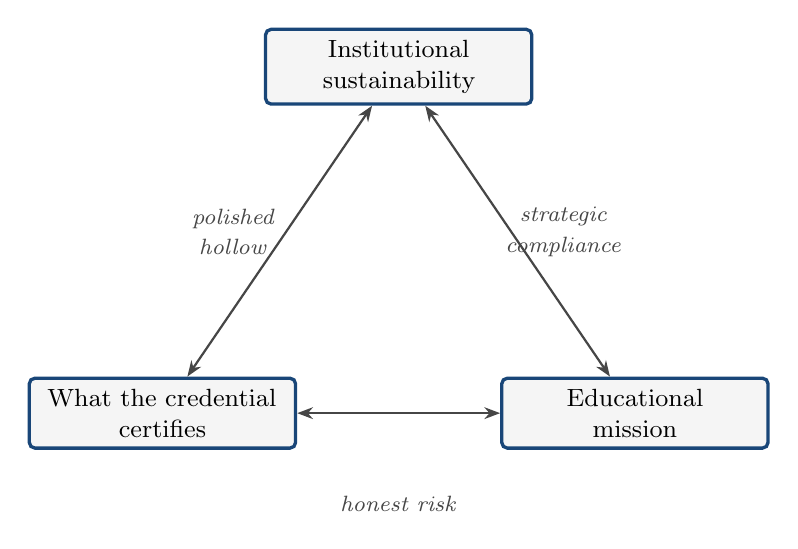
\begin{tikzpicture}
\node[emphasis-node, minimum width=3.3cm, minimum height=0.85cm, align=center, text width=3.1cm]
  (isustain) at (0, 2.9) {Institutional\\sustainability};
\node[emphasis-node, minimum width=3.3cm, minimum height=0.85cm, align=center, text width=3.1cm]
  (icred) at (-3.0, -1.5) {What the credential\\certifies};
\node[emphasis-node, minimum width=3.3cm, minimum height=0.85cm, align=center, text width=3.1cm]
  (imission) at (3.0, -1.5) {Educational\\mission};
\draw[bidir-arrow] (isustain) -- (icred);
\draw[bidir-arrow] (isustain) -- (imission);
\draw[bidir-arrow] (icred) -- (imission);
\node[caption-text, align=center, text width=2.8cm] at (-2.1, 0.8)
  {\footnotesize\textit{polished\\hollow}};
\node[caption-text, align=center, text width=2.8cm] at (2.1, 0.8)
  {\footnotesize\textit{strategic\\compliance}};
\node[caption-text, align=center, text width=2.8cm] at (0, -2.65)
  {\footnotesize\textit{honest risk}};
\end{tikzpicture}
\caption{\textbf{The Institution's Trilemma.} The same tension in inverted form at the institutional scale. Each edge labels the failure mode that arises when the two adjacent goals are kept at the cost of the third. This mirrors the Student's and Instructor's Trilemmas (\cref{fig:honest-a-bind,fig:instructor-trilemma}).}
\label{fig:institution-trilemma}
\end{figure}

Call this the \keyterm[Trilemma!Institution's]{Institution's Trilemma} (\cref{fig:institution-trilemma}). The corners are:

\begin{description}
\item[Institutional sustainability.] Keeping the institution financially viable through enrollment quality and quantity, tuition, donor cultivation, research grant flow, and state appropriations, and keeping the public legitimacy that makes financial viability possible. Public skepticism erodes enrollment; falling enrollment erodes funding; falling funding erodes the institution's ability to make the case for its own value \citep{insidehighered2026presidents}. Administrators cannot work on one face of this without working on the other.

\item[What the credential certifies.] The degree as a meaningful claim about the institution's graduates: what they can do, what they understand, why they are worth hiring or admitting to graduate school. The credential's value depends on both the institution's testimony (what it says its graduates can do) and the underlying evidence (what they can actually do under direct examination). When AI assistance enters student work without being verified, testimony and evidence drift apart.

\item[Educational mission.] The deeper commitment to what students gain by attending. This varies by institutional type (Jesuit formation, liberal arts breadth, research apprenticeship, workforce readiness, professional preparation) but is always present in the institution's self-understanding and almost always present in the language it uses to describe itself publicly. The mission is what an administrator points to when asked why the institution exists beyond its operational and credentialing functions.

What unifies these institution-type-specific articulations is a single claim: that some learning is itself the payoff, not just a means to an end. A coder welcomes AI because for them the drudgery is what they want eliminated and the working program at the end is the payoff. An artist resists AI because for them the drudgery, the patient hours of practice and revision, \emph{is} the payoff and the finished piece is its trace. The educational-mission corner rests on the same distinction at the institutional scale. An institution that has accepted that all of its content can be delivered more efficiently by AI has tacitly accepted that nothing it does is itself the point. An institution that defends its educational mission is asserting the opposite: that some of what students pay for, and some of what graduates carry forward, is the intellectual practice itself, not just its end product.
\end{description}

Each pair of corners can be satisfied at the cost of the third. The failure modes echo the Student's Trilemma deliberately.

\subsection{Three institutional failure modes}
\label{u:subsec:trilemma-failures}

\textit{Sustainability and credential certification without mission.} The institution maintains enrollment and credential reputation by becoming a sophisticated AI-gatekeeping operation. Students complete coursework, get verified through carefully designed oral defenses, receive degrees that mean what they say. But the institution has stopped trying to genuinely educate, in the sense the mission language implies, beyond the credentialing process itself. Call this the \keyterm[polished hollow!institutional]{institutional polished hollow}, a loss of mission: the credential is intact, the public-facing story is intact, but the educational mission has hollowed out from inside. This is the failure mode of an institution that has outsourced the deep work of education to AI while retaining institutional gatekeeping for itself.

\textit{Sustainability and mission without credential certification.} The institution maintains enrollment and stays committed to its educational mission, but lets AI-assisted work into the credential without demanding genuine ownership. Students graduate with degrees they cannot defend. The mission language remains genuine; the financial picture remains stable; the credential loses its meaning. This is the \keyterm[strategic compliance!institutional]{institutional strategic compliance}, a loss of credential integrity: the institution complies with the appearance of its credential function while quietly admitting that the verification was not done. This is the failure mode of an institution that wants to grow and stay true to its mission, but cannot bring itself to enforce the standards its credential implies.

\textit{Credential certification and mission without sustainability.} The institution stays rigorous and mission-driven, refuses to lower standards in response to AI pressure, and runs out of students or money in the process. Call this the \keyterm[honest risk!institutional]{institutional honest risk}, a loss of sustenance: every commitment kept, no commitment surrendered, but the institution cannot keep the doors open. This is the failure mode most visible at the moment among small private tuition-dependent colleges that have closed in the three years before this writing.

AI did not create the Institution's Trilemma any more than it created the Student's. The trilemma describes a structural tension that pre-existed AI and that any responsible institution always navigates. What AI did was sharpen each edge. Each pair of corners is harder to hold together when AI assistance lowers the apparent cost of giving up the third.

Most institutional AI policies published so far do one thing. They forbid passing off AI work as your own. That is worth doing, and it settles less than it appears to. A student can follow such a policy exactly, disclose every use, and still finish a degree without having learned what the degree says they learned. Honesty and understanding are different questions, and only one of them is what the credential certifies. A policy that reaches the first and stops has left the corner it most needed to defend.

\subsection{How the trilemma manifests differently by institutional type}
\label{u:subsec:trilemma-by-type}

The three corners are universal among degree-granting institutions, but the pull strength on each corner differs by institutional type. Four types are worth distinguishing, with the understanding that real institutions often combine features of more than one.

\textit{R1 private research universities.} At institutions like Stanford, Duke, and Tulane, sustainability is cushioned by endowments and tuition-pricing power, though research grant funding is, as of this writing, under direct AI strain: agentic-AI-assisted proposals are overwhelming funding agencies, which respond with submission caps and centralized review that reshape who gets funded \citep{rees2026agentic}. The credential is the brand; protecting it is non-negotiable. Mission is articulated through the dual commitment to research training and undergraduate liberal education. Where these conditions hold, the institutional polished-hollow failure mode is the one to watch: an institution that maintains its credential through sophisticated gatekeeping while quietly admitting that what it offers undergraduates has converged with what AI tutors offer for free.

\textit{Wealthy liberal arts colleges.} At institutions like Williams, Pomona, and Kenyon, the trilemma takes its tightest form. Credential and mission corners are tightly coupled: the case for the institution \emph{is} the case for the human-led residential experience. Sustainability is the threatening corner. With small enrollments and tuition dependence, the institutional honest-risk failure mode is the most visible and the most current. The closures of small private tuition-dependent colleges in the years leading up to this writing follow this pattern \citep{levine2026upheaval}. The case for these institutions in the AI era is not that they teach better content than larger universities, since AI tutors can deliver content well. It is that they teach in a setting where the human-led mentoring relationship is the educational point, not just the delivery mechanism.

\textit{Regional public universities.} At most state-system institutions outside the research-flagship tier, sustainability dominates. The enrollment cliff hits hardest at this institutional type, and federal-plus-state funding cuts compound the pressure. Educational mission is increasingly framed in workforce-alignment terms rather than liberal-education terms, partly in response to state legislatures and partly in response to student-and-parent demand for clear post-graduation outcomes. Credential certification matters operationally (graduates need to perform when they leave) but is rarely the primary strategic conversation. Where enrollment pressure dominates like this, the institutional strategic-compliance failure mode tends to be the primary risk: an institution that maintains enrollment by accepting AI-assisted work without demanding genuine ownership, because the cost of demanding genuine ownership is enrollment the institution cannot afford to lose.

\textit{Community colleges.} The trilemma is flatter here. Public trust in community colleges has remained strong even as trust in higher education broadly has eroded; one common explanation, offered by DeRionne Pollard, who leads the American Association of Community Colleges, is that community colleges are seen as affordable, career-pathway-connected, and engaged with local employer needs \citep{pollard2026community}. Sustainability pressure exists but is less acute. The mission corner is more clearly articulated as access plus workforce alignment than at other institutional types. The credential corner is dominated by a different question (credit transferability to four-year institutions) than at other types. Among the three failure modes the framework names, the one community colleges seem least vulnerable to is the honest-risk pattern; they are more vulnerable to local-mission drift if state policy shifts.

The four types are not comprehensive. Specialized institutions (HBCUs, religious-affiliated colleges, for-profit institutions, fully online providers) face the same trilemma but with type-specific pull strengths on each corner. The framework's value is that the corners stay the same; what changes is the relative pull and the failure mode most likely to materialize.

\subsection{Why the Institution's Trilemma matters for the rest of this Part}
\label{u:subsec:trilemma-stakes}

The institutional policies developed in the rest of this Part (the assessment models, the integrity procedure, the faculty change-management approach, the implementation phases) are tools for holding the three corners of the trilemma together under AI pressure. Without the trilemma frame, these tools can read as a list of operational responses to a list of operational problems. With the trilemma frame, they read as coordinated commitments that protect the institution from each of the three failure modes simultaneously. The trilemma is managed, not solved: no fixed point dissolves the tension. The healthy state is holding all three corners in dynamic balance, the way a three-legged stool needs all three legs and no single leg is the optimum.

This Part also has a more concrete rhetorical purpose\index{department chairs!argument to deans}. Department chairs and program directors increasingly find themselves in conversations with deans, provosts, and boards about whether faculty roles can be replaced by AI tools at substantially lower cost. The Institution's Trilemma supplies the structural answer to that question: the case for human-led education is the case that the educational-mission corner cannot be honored by a system that has hollowed out into pure credentialing. This view is consistent with the OECD's analysis of teaching in the age of AI, which holds that AI amplifies both effective and ineffective educational practice and that the teacher's judgment and human qualities remain central, particularly where the technology has clear limits \citep{schleicher2026quality}. Throughout the rest of this Part, those same operational tools can be read as ammunition for the argument chairs need to make to deans when AI-replacement proposals arrive on the agenda. The argument is not nostalgic and it is not defensive. It is the argument that some of what students pay for, and some of what graduates carry forward, is the very thing that AI-as-replacement is supposed to eliminate.

A budget model can quietly undercut\index{Responsibility Center Management}\index{budget incentives}\index{enrollment pressure} the standards an institution says it wants to keep. Under Responsibility Center Management (RCM) and similar models, a unit's resources rise and fall with its enrollment. A department that allows broader AI use may then pull students from a department that holds a stricter line. The pool of students is roughly fixed, so one unit's gain is another's loss. That leaves the stricter unit financially punished for the very standard the institution endorses. Each unit then has reason to loosen in turn. The result can be a slow drift toward the most permissive policy on offer, and no single department can step out of it alone. The same pressure runs one level down, between instructors: the colleague who is generous with AI may draw students from the one who is not. None of this comes from any unit's bad choice; it comes from how the budget is built. So it can be fixed only where the budget is set. An institution that wants its standards to hold should set the core expectations centrally and stay alert to its own budget incentives, so departments are not left competing on permissiveness. This risk appears among those tracked in the Risk register (\cref{u:sec:risk-register}).

The Northeastern case discussed in the next section can be read through the trilemma frame. It is not just a faculty integrity question. It is an early signal of the institutional polished-hollow pattern: an institution that maintained its credential and sustainability through procedural responses to a violation, but did not address the deeper mission question of what students were paying for.

\section{The institutional problem}
\label{u:sec:problem}%
\index{institutional problem}

\bookepigraph{AI can deliver the facts.\\An education forms the values and judgment to use them.}

A senior at Northeastern University spent the final weeks of her undergraduate degree filing a formal complaint and a tuition refund request against her organizational behavior professor. She had discovered that the professor was using ChatGPT, Perplexity, and an AI presentation generator to produce her lecture materials, with a stray AI prompt instruction visible in the slides. The syllabus for the course prohibited student AI use. The professor later acknowledged the AI assistance. The university declined to refund the tuition.\footnote{\citet{hill2025professors}.}

The case names a pattern. The professor was wearing a \keyterm{competence costume}: AI-polished material that signals more current and confident engagement than the underlying work supports. The student saw it. The institution declined to act on it. The asymmetry is the point. An integrity rule that applies to students but not to those teaching them is structurally fragile.

In the language of Part~\ref{part:student} (\cref{subsec:trilemma-failures}), the Northeastern professor's costume was projected through \emph{strategic compliance}: he understood his own course but hedged on disclosure. \emph{Competence costume} names the outward projection; the taxonomy names the configuration that produces it.

The translation test introduced for students in Part~\ref{part:student} (\cref{sec:compact}) gives institutions a positive standard to adopt symmetrically. Faculty who use AI assistance in course materials should be able to translate those materials into their own language and examples. Students using AI on coursework should be able to do the same. The same diagnostic, applied to both, is a policy the institution can defend in public.

AI creates a gap between polished performance and demonstrated learning. A student may submit fluent prose, working code, or a convincing solution without having developed the underlying competence. This problem is not limited to cheating. It can happen through ordinary over-reliance. A student may believe they understand because the final product looks good.

The institutional response should not be to treat every AI-assisted product with suspicion. The better response is to redesign expectations. Courses should assess both independent understanding and responsible tool use. Students should learn to verify, disclose, and defend AI-assisted work. Faculty should have clear models for small, medium, large, and online courses. Departments should not leave each instructor to invent policy alone.

The goal is a durable approach. AI systems will become stronger. Detection tools will remain imperfect. The safest assessments will be those that make student thinking visible and require students to explain, verify, apply, and revise their work.

Evidence from learning science supports this direction. Practice testing and distributed practice have strong support across learning contexts, and recent AI-tutoring studies suggest that carefully designed systems can help when they preserve active engagement rather than replace it \citep{dunlosky2013improving,kestin2025ai}. At the same time, field evidence warns that unrestricted generative AI can create short-term performance gains without durable learning \citep{bastani2025generative}.

\section{Guiding principles}
\label{u:sec:principles}%
\index{guiding principles}

The following principles should guide institutional policy.

\begin{enumerate}
  \item \textbf{Learning remains the center.} AI may support learning, but it should not replace the intellectual work students are meant to practice.
  \item \textbf{Independent competence must be preserved.} Every course should identify what students must be able to do without AI or with tightly bounded support.
  \item \textbf{AI literacy is a legitimate educational goal.} Students should learn how to use AI critically, productively, and ethically within their disciplines.
  \item \textbf{Verification is required.} AI output should be treated as provisional until checked against evidence, data, sources, methods, or disciplinary standards.
  \item \textbf{Disclosure should be normal, brief, and useful.} Students should know how to describe what AI contributed and what they verified.
  \item \textbf{Assessment should reveal thinking.} Courses should gather evidence of reasoning, process, revision, judgment, and transfer, not only polished final products.
  \item \textbf{Privacy and equity must be protected.} Students should not be required to use tools that compromise data, create avoidable costs, or disadvantage students by language background, disability, access, or prior exposure.
  \item \textbf{Faculty judgment remains human.} AI may help instructors prepare feedback and materials, but instructors remain responsible for grades, academic-integrity judgments, student evaluation, and the accuracy and integrity of the materials they put before students.
\end{enumerate}

These principles align with emerging international guidance that treats AI literacy, human oversight, ethics, privacy, and responsible educational design as central institutional responsibilities \citep{miao2023guidance,miao2024aia,miao2024aib,europeancommission2022ethical,oecd2026digital}.

\chapter{The Framework and Vocabulary}
\label{u:ch:the-framework-and-vocabulary}%

\section{The CAT framework}
\label{u:sec:cat}%
\index{CAT framework}

University policy should distinguish three kinds of learning evidence: Core Competence, AI-assisted Practice, and Trustworthiness. The acronym CAT gives faculty and students a shared language.

\begin{description}
  \item[Core Competence.] What students must understand and be able to do without AI or with tightly bounded assistance.
  \item[AI-assisted Practice.] What students can do when they use AI responsibly as a permitted tool for learning, revision, analysis, coding, feedback, or exploration, without losing control of the work. In institutional policy this includes AI acting as tutor, critic, simulator, editor, coding aid, or research assistant.
  \item[Trustworthiness.] How well students verify, disclose, critique, and take ownership of AI-assisted work.
\end{description}

The distinction matters because these abilities can diverge. A student may produce strong AI-assisted work while having weak independent understanding. Another student may understand the material well but use AI carelessly. Good policy should not collapse these into one score.

Institutional guidance should therefore encourage courses to state which assignments measure Core Competence, which assignments develop AI-assisted Practice, and which assignments evaluate Trustworthiness. The student-facing development of the framework appears in Part~\ref{part:student} (especially~\cref{sec:cat}); the instructor-facing development appears in Part~\ref{part:instructor} (especially~\cref{i:sec:cat-framework}). Graduate programs adopting the framework directly should consult Appendices~\ref{app:gmip} and~\ref{app:mae}.

A single assessment can serve more than one of these. A closed-book exam measures Core Competence; an AI-permitted assignment develops AI-assisted Practice; a project that students present and then answer questions about does both at once, since the artifact reflects AI-assisted Practice while the live questioning tests Core Competence and Trustworthiness together. The categories name what an assessment measures, not a rule that each measure only one thing.

\subsection{Alignment with UNESCO learning outcomes}
\label{u:subsec:unesco-outcomes}

UNESCO's guidance \citep{miao2023guidance} proposes four broad categories of learning outcomes that universities should consider as they revise curricula for the AI era: \emph{values} that ensure human-centred design and use of technology; \emph{foundational knowledge and skills} (literacy, numeracy, basic scientific literacy) that remain prerequisites even when AI can perform specific tasks better than humans; \emph{higher-order thinking skills} that ground critical evaluation of AI output and human-AI collaboration; and \emph{vocational skills} required to work with AI systems in domains where AI is automating task units. The CAT framework above is consistent with all four. Core Competence corresponds to foundational knowledge and skills; Trustworthiness corresponds to values and to the critical-evaluation dimension of higher-order thinking; AI-assisted Practice corresponds to vocational skills and to the human-AI-collaboration dimension.

Together with the student-framework crosswalk (\cref{tab:cat-unesco}) and the teacher-framework crosswalk (\cref{tab:instructor-unesco}) established earlier in this volume, the institutional framework here translates cleanly onto UNESCO's structure for accreditation reporting, curriculum-revision proposals, and international-collaboration framing. National-policy environments outside UNESCO alignment can perform analogous mappings against their own framework documents \citep{usde2023artificial}; the CAT structure is intended to translate cleanly onto most national or regional frameworks rather than to compete with them. As universities revise curricula in the years ahead, this UNESCO categorization may prove a useful framework-independent reference point.

\subsection{Accreditation and assurance of learning}
\label{u:subsec:accreditation}%
\index{accreditation}

The framework's distinction between Core Competence and AI-assisted Practice connects directly to accreditation, which is where assessment policy acquires institutional force. Both institutional accreditors, which review the university as a whole, and programmatic accreditors, which review specific degrees, ask the same underlying question: can the institution show that students actually achieve the learning outcomes it claims? Engineering and computing programs answer to ABET, business programs to AACSB, and many health, education, and other programs to their own disciplinary bodies, but the logic is shared across all of them.

AI sharpens this question rather than changing it. Where a stated outcome requires a competence students must hold independently, the institution must be able to show that the outcome was assessed independently of AI, not inferred from work that AI could have produced. The Minimum independent-competence requirement (\cref{u:sec:min-competence}) is the mechanism that supplies this evidence, and the CAT distinction lets a program report cleanly on which outcomes are assessed as independent competence and which are assessed as responsible AI-assisted practice. A program that maps its outcomes onto CAT can show an accreditor not only what it teaches but how it knows students learned it under current conditions.

The practical implication for departments is to treat AI-aware assessment design and accreditation reporting as a single activity rather than two. An assessment plan that already separates independent competence from AI-assisted practice produces the evidence an accreditor expects, and the UNESCO crosswalks described above (\cref{u:subsec:unesco-outcomes}) give institutions in those policy environments a ready translation for the reporting itself.

\section{Shared vocabulary}
\label{u:sec:vocabulary}%
\index{glossary!Part III}%
\index{shared vocabulary}

A common vocabulary reduces confusion across courses. The following terms should be used consistently in university policy. The vocabulary appears here at the start of the Part, rather than in an end glossary, because policy writing quotes its definitions up front.

\begin{description}
  \item[Core Competence.] What students must understand and be able to do without AI or with tightly bounded assistance.
  \item[AI-assisted Practice.] What students can do when they use AI responsibly as a permitted tool for learning, revision, analysis, coding, feedback, or exploration, without losing control of the work.
  \item[Trustworthiness.] How well students verify, disclose, critique, and take ownership of AI-assisted work.
  \item[No-AI work.] Work completed without AI assistance, except for accommodations or tools explicitly approved by the instructor.
  \item[Bounded-AI work.] Work completed with limited, specified AI assistance, such as a single approved tool, a restricted prompt type, or a fixed time window.
  \item[Open-AI work.] Work in which students may use AI broadly, subject to disclosure, verification, and course rules.
  \item[AI-assisted work.] Student work improved with AI support but written, verified, and owned by the student.
  \item[AI-generated output.] Text, code, images, explanations, summaries, solutions, data analyses, or other content produced by an AI system.
  \item[Assessment validity.] The degree to which an assessment measures the competence it claims to measure. Distinct from reliability (consistency of measurement) and fairness (procedural justice in the assessment process).
  \item[Institution's Trilemma.] The three-way pull among institutional sustainability, what the credential certifies, and the educational mission. Keeping any two at the cost of the third produces the institutional polished hollow (a loss of mission), institutional strategic compliance (a loss of credential integrity), or institutional honest risk (a loss of sustenance).
  \item[Competence costume.] AI-polished material that signals more current and confident engagement than the underlying work supports.
  \item[Disclosure.] A factual statement of which tools were used, what they contributed, and how the student verified the result.
  \item[Verification.] The process of checking AI output against course materials, sources, data, code tests, experiments, professional standards, or independent reasoning.
  \item[Process evidence.] Artifacts that show how work was produced, such as plans, drafts, prompt logs, version histories, verification notes, source checks, lab notebooks, or code tests.
  \item[Oral defense.] A live explanation in which students answer questions about their work, reasoning, sources, methods, or AI use.
  \item[Random audit.] A routine assessment check in which a student is asked to explain or verify submitted work. It is not, by itself, an accusation.
\end{description}

\section{Course-level AI-use categories}
\label{u:sec:categories}%
\index{course-level AI-use categories}

Every assignment should state what kind of AI use is allowed. The following four categories are simple enough for students and flexible enough for departments.

These are the same four categories developed in Parts~\ref{part:student} and~\ref{part:instructor}, restated here as shared institutional vocabulary so that this Part can stand on its own; readers who have met them already can skim the definitions.

The boundaries between categories are not always sharp. A student who asks AI to explain an approach and then to help draft from that explanation has moved from tutor to collaborator within one session. The categories name the dominant role AI plays in producing the submitted work. Each assignment should state which role is permitted, and where a task genuinely mixes roles, the instructor should say so rather than force an artificial split.

\subsection{\texorpdfstring{\NAI{}: No AI}{NAI: No AI}}
\label{u:subsec:red}

AI use is not allowed. These assignments measure independent competence. Examples include closed-book exams, in-class writing, oral explanations, live coding checks, foundational calculations, language practice, and lab practicals.

NAI assignments should not dominate every course. They serve a specific purpose: they show what students can do without external scaffolding.

\subsection{\texorpdfstring{\AIT{}: AI as Tutor}{AIT: AI as Tutor}}
\label{u:subsec:yellow}

AI may be used for explanation, practice, review, hints, and study support, but not to produce submitted work. A student might ask AI to explain a concept, generate practice questions, or quiz them before an exam. The submitted response should still be the student's own unaided work.

\subsection{\texorpdfstring{\AIC{}: AI as Collaborator}{AIC: AI as Collaborator}}
\label{u:subsec:green}

AI may help with brainstorming, drafting, revising, debugging, outlining, critique, source search, comparison, or testing. Students must disclose use and verify important claims. AIC assignments are useful when the course goal includes revision, professional practice, coding, research, modeling, or design.

\subsection{\texorpdfstring{\AIS{}: AI as Object of Study}{AIS: AI as Object of Study}}
\label{u:subsec:blue}

Students analyze AI output directly. They may identify hallucinations, critique bias, compare tools, repair flawed reasoning, evaluate generated code, examine source quality, or test how AI performs in a discipline. AIS assignments teach students to examine AI rather than merely use it.

\section{Assessment models by course size}
\label{u:sec:models}%
\index{assessment models}

Class size changes what assessment can reasonably do. The same principles apply across courses, but the implementation must differ.

\subsection{Oral-Defense Model}
\label{u:subsec:oral-defense}

The Oral-Defense Model is best for small classes of any level: seminars, honors courses, capstones, writing workshops, advanced labs, research courses, and many graduate courses. The model is class-size-driven; it works wherever instructors can speak directly with each student about their work.

Students may use AI more extensively when they can be asked to defend what they submitted. A defense may be a board proof, source-analysis conversation, code walk-through, lab-method explanation, design critique, writing conference, or project presentation.

A course using this model should include at least one live explanation of AI-assisted work. The purpose is not to intimidate students. It is to confirm ownership and deepen learning. The operational treatment of this model, including recommended structure, a worked example, suggested weighting, and equity considerations, appears in Part~\ref{part:instructor} (\cref{i:sec:oral-defense-model}).

\subsection{Evidence-of-Thinking Model}
\label{u:subsec:evidence-thinking}

The Evidence-of-Thinking Model is best for large lectures, service courses, online courses, and multi-section courses. In these settings, individual oral exams for every student may not be feasible.

Large courses should gather repeated, low-cost evidence of thinking. Useful tools include short no-AI quizzes, in-class writing, draft histories, source checks, process logs, AI-use disclosures, homework-to-quiz transfer questions, flawed-output critiques, code tests, lab notebooks, short video explanations, and random oral audits.

The goal is not surveillance. The goal is valid assessment. A polished final product is no longer enough evidence by itself. The operational treatment of this model, including scalable evidence sources, a worked example, suggested weighting, and random oral audits, appears in Part~\ref{part:instructor} (\cref{i:sec:evidence-model}).

\subsection{Hybrid Model}
\label{u:subsec:hybrid}

Many courses are too large for full oral exams but small enough for some live explanation. The Hybrid Model combines scalable process evidence with limited direct questioning. It may use group oral exams, sampled oral audits, TA-led conferences, short instructor meetings, video explanations, and written verification logs.

Hybrid designs are useful for medium-sized writing courses, upper-level STEM courses, lab courses, project-based courses, and professional programs. The operational treatment of this model, including a recommended structure with mapping table, sampling strategy for live audits, a worked example, and suggested weighting, appears in Part~\ref{part:instructor} (\cref{i:sec:hybrid-model}).

\begin{table}[htbp]
  \centering
  \caption{\textbf{Recommended assessment model by course context.} The model follows from how much direct contact with each student the course allows. Where contact is high, as in a seminar, an oral defense verifies understanding directly. Where it is low, as in a large lecture or an online section, the evidence has to be built into the work itself.}
  \label{u:tab:course-models}
  \begin{tabularx}{\textwidth}{>{\raggedright\arraybackslash}X>{\raggedright\arraybackslash}X}
    \toprule
    Course context & Recommended model \\
    \midrule
    Small seminar & Oral-Defense Model \\
    Graduate course & Oral-Defense or Hybrid Model \\
    Honors course & Oral-Defense or Hybrid Model \\
    Medium undergraduate course & Hybrid Model \\
    Large lecture & Evidence-of-Thinking Model \\
    Multi-section course & Evidence-of-Thinking Model with TA calibration \\
    Online course & Evidence-of-Thinking Model with stronger process documentation \\
    Capstone or project course & Hybrid or Oral-Defense Model \\
    \bottomrule
  \end{tabularx}
\end{table}

\Cref{u:tab:course-models} names the primary model for each context, not the only one in play. Most courses combine elements: a small seminar built on oral defense still gathers some written process evidence, and a large lecture using the Evidence-of-Thinking Model can still sample a few oral audits. Read each recommendation as a course's center of gravity, not an exclusive choice.

\chapter{Standards and Requirements}
\label{u:ch:standards-and-requirements}%

\section{Minimum independent-competence requirement}
\label{u:sec:min-competence}%
\index{minimum independent-competence requirement}

Every course should include some meaningful assessment of what students can do independently. The form should fit the discipline.

In STEM courses, this may be a quiz, exam, derivation, lab practical, coding check, or oral explanation. In writing courses, it may be in-class writing, a writing conference, or a revision defense. In humanities courses, it may be close reading, source analysis, or argument reconstruction. In professional programs, it may be a case explanation, simulation, or ethical decision defense.

The institution should not prescribe one method for every course. It should prescribe the principle: some course credit should reflect independent understanding, not only AI-assisted production.

A useful policy sentence is:

\begin{quote}
Every course should identify the core skills, concepts, or judgments students must demonstrate without AI or with tightly bounded assistance. The method of assessment should be appropriate to the discipline, level, enrollment, and learning goals of the course.
\end{quote}

\section{Disclosure standard}
\label{u:sec:disclosure}%
\index{disclosure!standard}

Disclosure should be normal and brief. It should not read like a confession. It should give instructors enough information to understand how AI shaped the work.

Disclosure attaches to AI use that shapes the substance, structure, or analysis of the work, not to routine mechanical help. Spelling correction, grammar checking, and predictive text are treated like the familiar tools they resemble and need not be reported, just as using a calculator or a dictionary is not. The question is not whether software touched the work but whether it did any of the thinking the assignment is meant to develop.

A recommended student disclosure block is:

\begin{quote}
\textbf{Tools used:} Name the tools used, if any.\\
\textbf{Tool role:} Describe what the tools helped with.\\
\textbf{Student role:} Describe what you wrote, revised, checked, or decided.\\
\textbf{Accepted, changed, or rejected:} Describe the AI contributions you used, revised, or set aside.\\
\textbf{Independent verification:} Describe how you checked important claims, sources, data, code, or reasoning.\\
\textbf{What I can explain without AI:} Name the main parts of the work you can now explain on your own.
\end{quote}

A complete entry need not be long. A student who used AI to help debug a script might capture all of this in a few lines. The AI assistant suggested fixes for a sorting bug. The student wrote the original code, applied the fix, and added tests, then kept the fix but renamed the variables. They confirmed the result with a minimal working example, and they can explain the sorting logic and why the bug occurred without AI.

The depth of disclosure should track what the course treats as core. A student may use a tool below the course's core level as a black box without explaining its internals. In a course where nonlinear optimization is a means rather than a learning goal, it is enough to report that an optimizer was used and verified, without accounting for how the optimizer works. Where a tool touches the core competence the course is meant to build, the explanation should reach that level. The same habit of naming the help received applies to substantial non-AI assistance wherever a course's policy already calls for it.

For low-stakes assignments, a one-sentence disclosure may be enough. For substantial AI-assisted projects, instructors may require a process log, prompt excerpts, verification notes, or a short reflective memo.

\section{Privacy, data governance, and tool approval}
\label{u:sec:privacy}%
\index{privacy and data protection}\index{data governance}\index{tool approval}

Students and faculty need clear rules about what may not be uploaded into AI systems. These rules should be plain enough to appear in syllabi and student orientation materials.

Unless a tool has been approved for the specific use, students and faculty should not upload:

\begin{itemize}
  \item private information about students, classmates, patients, clients, research subjects, or employees;
  \item unpublished research data without permission;
  \item restricted exams, answer keys, or secure assessment materials;
  \item confidential institutional documents;
  \item private correspondence, recommendation letters, or evaluations;
  \item copyrighted course materials when sharing is not permitted;
  \item data governed by human-subjects, clinical, contractual, or legal restrictions.
\end{itemize}

The institution should maintain a list of approved tools and approved uses. A tool approved for general brainstorming may not be approved for student records, research data, grading, or protected course materials.

Data governance should also address retention, training use, third-party access, accessibility, cost, procurement, and support. These details should not be left to individual instructors alone.

One more category belongs here, and it is easy to miss: regulation. AI that makes or supports decisions about students may be regulated activity, not merely a matter of institutional policy. Admissions, assessment, and monitoring are the uses that draw attention. Obligations can include bias testing, documented human oversight, and retained records. Some regimes reach across borders. Institutions should confirm where they stand with counsel, and the companion repository maintains a current orientation (\texttt{institutions/regulatory-landscape.md}).

When a course requires students to share their AI conversation threads with the instructor as part of an integrity practice (see Part~\ref{part:instructor} \cref{i:subsec:required-mentor}), those threads become a new category of student work that institutional data governance should address explicitly. The thread is the student's contribution to the assignment, so retention rules should mirror those for other student work. The thread may also contain sensitive information the student shared with the AI (course frustrations, learning struggles, off-topic personal disclosures). The data governance policy should set expectations for how shared threads are handled by faculty and TAs, who has access, how long they are retained, and what happens to them at course end. Departments and institutions adopting the required-mentor-prompt practice should align retention and access protocols with their existing protections for other student work and with applicable privacy law in their jurisdiction (FERPA in the United States; equivalent frameworks elsewhere).

\section{Equity, access, and accessibility}
\label{u:sec:equity}%
\index{equity and access}

AI policy should avoid creating a hidden paywall around learning. If a course requires AI use, students should have access to an approved tool at no additional cost or should be offered an equivalent alternative.

Equity also includes language background, disability, prior exposure, bandwidth, device access, and confidence using new tools. Some students will arrive with extensive AI experience. Others will be learning basic use for the first time. Courses should not mistake unequal access for unequal ability.

Survey evidence puts numbers on that unevenness. Regular AI use was reported by about a third of women against nearly half of men, and by under a third of underrepresented minority students against roughly two fifths of White and Asian students \citep{chirikov2026generative}. The authors are careful about what this shows. Higher use is not better use. The concern is that unequal engagement becomes unequal opportunity to build the literacy and the critical oversight this framework asks of every graduate.

Accessibility can cut in both directions. AI tools may help some students summarize, rephrase, plan, or review material. They may also create barriers if tools are inaccessible, expensive, unstable, or poorly documented. Accommodation decisions should remain human and should follow institutional disability procedures.

The institution should also be careful with AI detectors. Evidence shows that some detectors misclassify writing by non-native English writers as AI-generated, raising concerns about fairness and reliability \citep{liang2023gpt}. For that reason, detection scores should not be treated as primary evidence of misconduct.

\section{Academic integrity procedure}
\label{u:sec:integrity}%
\index{academic integrity!procedure}

Academic integrity should be handled through evidence and due process, not through detector scores alone. A fair procedure should distinguish misunderstanding from deliberate misconduct. Early empirical work on ChatGPT and student writing emphasized that anticipatory course design and explicit policies are more effective than detection-driven enforcement \citep{cotton2024chatting}.

The case against detector-based enforcement is now quantitatively documented. \index{Liang detector study}Liang and colleagues evaluated seven widely used GPT detectors on TOEFL essays written by non-native English speakers \citep{liang2023gpt}. The average false-positive rate was 61.3\%. All seven detectors unanimously misclassified 19.8\% of the essays. At least one detector flagged 97.8\% of them as AI-generated. The mechanism is identifiable: most current detectors rely on text perplexity, a measure of how predictable a sequence of words is to a language model, and non-native writers exhibit lower lexical and syntactic variability that produces lower perplexity that detectors then read as AI-generated. The same study shows that detectors can be bypassed by prompting an AI to use more literary language, with detection rates falling to near zero. Detectors therefore fail in two directions, and both directions disadvantage students who can least afford the error: false positives concentrate on multilingual writers, and false negatives accrue to students with the resources and skill to refine prompts. These rates come from the detector tools available in 2023. Later detectors may lower the false-positive rate. The structural problem will remain. Perplexity-based detection penalizes non-native writers by design, and that will not change without a fundamental change in how detection works.

Beyond accuracy, detector-based enforcement produces what those authors term a presumption of guilt, an institutional posture in which automated systems flag students as suspect and the burden falls on them to prove innocence; the reputational consequences of a flagged accusation may persist even when the accusation is later revoked.

The accuracy concerns translate into harm at the case level. A senior at the University of California Davis whose paper was flagged by Turnitin as AI-generated spent the final months of her senior year defending against the accusation; her grades reportedly began to slide as she fought it.\footnote{\citet{klee2023falsely}.} The arms race that detector reliance creates has produced its own absurdity. Students now use ``humanizer'' tools that adjust AI-generated text to defeat detection, and some students who do not use AI at all subscribe to the same tools to reduce the chance of being falsely flagged. As one professor quoted in recent reporting put it, the better the writer you are, the more AI thinks you're AI.\footnote{\citet{kingkade2026avoid}; the line is attributed in that article to Erin Ramirez of California State University, Monterey Bay.} Detector dependence does not create the integrity problem. It produces a parallel problem of its own.

A recommended process is:

\begin{enumerate}
  \item Review the assignment rules and the student's disclosure.
  \item Examine process evidence, such as drafts, version history, source notes, lab notebooks, code history, or prompt logs.
  \item Compare submitted work with in-class work when relevant.
  \item Invite the student to explain the work in a non-accusatory meeting or written response.
  \item Use a short reassessment or oral explanation when needed.
  \item Document the concern, evidence, student response, and decision.
  \item Use educational remedies for minor first violations when appropriate.
  \item Use formal academic-integrity procedures for serious, deceptive, or repeated misconduct.
\end{enumerate}

The institutional standard should be clear:

\begin{quote}
AI-detector output may be considered, if allowed by institutional policy, but it should not serve as the sole or primary evidence of academic misconduct. Decisions should rest on assignment rules, process evidence, student explanation, and professional judgment.
\end{quote}

\section{Faculty use of AI}
\label{u:sec:faculty-use}%
\index{faculty use of AI}

The framework applies to faculty as well as students, and it applies in full. Faculty may use AI to support teaching, but they remain responsible for professional judgment and they say where AI touched the work students receive. A course that asks students to disclose while the instructor does not has taught them that disclosure is a rule imposed on the assessed, not a habit of the profession.

The Northeastern case discussed in \cref{u:sec:problem} is one of the early reported instances where this responsibility was tested in public. The translation test offers an internal standard faculty can apply to themselves. A faculty member using AI assistance on a piece of course material should be able to translate the material into their own language, with their own examples, in their own structure, before placing it in front of students. If the translation is awkward, the integration is incomplete. A faculty member who cannot make that translation is wearing the competence costume the Northeastern case made visible.

Appropriate uses may include drafting examples, generating practice questions, identifying possible misconceptions, improving assignment wording, drafting feedback for human review, creating case variations, and preparing discussion prompts.

Faculty should not delegate final grades, academic-integrity decisions, accommodation decisions, or sensitive student evaluation to AI. They should not upload protected student work, student records, or confidential materials into unapproved systems.

A concise policy sentence is:

\begin{quote}
Instructors may use AI to assist teaching preparation and feedback drafting, but the instructor remains responsible for all grades, evaluative judgments, academic-integrity decisions, course materials, and protection of student information.
\end{quote}

\section{Required syllabus elements}
\label{u:sec:syllabus}%
\index{syllabus!required elements}

Every syllabus should answer five questions.

\begin{enumerate}
  \item What AI uses are allowed or prohibited in this course?
  \item Which assignments are NAI, AIT, AIC, or AIS?
  \item What must students be able to do without AI?
  \item How should students disclose AI use?
  \item What materials may not be uploaded into AI systems?
\end{enumerate}

Ready-to-adapt statements for each category, a general course statement, and an assignment-label template appear in Part~\ref{part:instructor} (\cref{i:app:syllabus}); a complete fill-in syllabus template appears in \cref{u:app:syllabus-template}.

For large or multi-section courses, syllabi should also explain how the course will check understanding. Examples include short no-AI quizzes, process logs, random oral audits, in-class writing, draft histories, or TA-led conferences.

Courses that adopt the required-mentor-prompt practice (Part~\ref{part:instructor} \cref{i:subsec:required-mentor}) should additionally answer two questions in their syllabus: how the mentor-prompt requirement applies (which assignments, with what scaffolding) and how shared conversation threads will be reviewed, retained, and protected. The institution's general AI data-governance policy (\cref{u:sec:privacy}) should be the floor; course-level commitments may go further but should not undercut institutional protections.

\chapter{Governance and Support}
\label{u:ch:governance-and-support}%

\section{Governance and support}
\label{u:sec:governance-support}%
\index{governance}

A framework needs both an owner and a way to reach students. Two structures separate a policy that lives on paper from one that changes practice: a body that owns the policy, and a support system that helps students and faculty act on it.

\subsection{Governance and oversight}
\label{u:subsec:governance}

Responsibility for AI policy is easy to misplace. The questions it raises, about what a course should certify, how to assess independent competence, and when AI use is honest, are academic and ethical rather than technical. Yet the natural institutional reflex is to route anything involving software to information technology. IT has an essential role in access, security, procurement, and data protection, but those are different questions from how AI changes learning and how to use it well. A policy left to IT tends to answer the questions IT is equipped to answer and to leave the academic ones unowned.

The more durable arrangement is a standing, cross-functional body that owns the policy. It is a committee or task force that includes academic leadership, faculty from more than one discipline (among them some who are skeptical of AI), students, and representation from information technology, the library, and legal counsel. Its remit is to maintain the institution's AI-use policy and shared vocabulary, to review and approve tools for specific uses (\cref{u:sec:privacy}), to monitor the risks in the register (\cref{u:sec:risk-register}), and to review the framework on the regular cycle the outcomes call for (\cref{u:sec:institutional-outcomes}). The policy itself should carry a date and a stated review cadence. An undated policy in a field moving this fast cannot be maintained, and after a year it reads as expired. The exact form should fit the institution. What matters is that the body exists, that it is led from the academic side rather than from IT, and that someone owns the policy rather than each office assuming another will. Such a body rarely starts from nothing; it usually builds on departments that have already developed coherent practice, the bottom-up pattern described in \cref{u:sec:dept-to-institution}.

\subsection{Support beyond the classroom}
\label{u:subsec:support}%
\index{support units}%
\index{library}

Owning the policy is not the same as helping students follow it. Much of the work of learning to use AI well happens outside any single course, in the units students already turn to for help. Coordinating those units rather than leaving each to improvise is what turns a policy into everyday support. The library is the natural hub for the student-facing part. Teaching information and research literacy is already its mandate \citep{acrl2016framework}, and evaluating AI-generated content, judging a tool's limits, and choosing the right tool for a task are direct extensions of that work. Other units carry the pieces closest to their own:

\begin{itemize}
  \item \textbf{The library} curates AI-literacy resources, runs workshops on effective and ethical use, helps students see which tools suit which tasks, and is a natural home for the required AI-literacy module (\cref{u:subsec:ai-literacy-requirement}).
  \item \textbf{Writing centers} help students use AI within the writing process without surrendering authorship, reinforcing the verification and disclosure habits the framework asks for.
  \item \textbf{Tutoring and academic-success centers} teach study strategies that use AI as a tutor rather than a substitute, complementing human tutoring rather than competing with it.
  \item \textbf{Academic advising} helps students understand course-level AI rules and plan for assessments of independent competence.
  \item \textbf{Disability and accessibility services} keep accommodation decisions and approved tools aligned, so that AI neither bypasses an accommodation nor becomes a barrier (\cref{u:sec:equity}).
\end{itemize}

Faculty support remains the work of the teaching center (\cref{u:sec:teaching-center}); the units above are where students meet the framework outside the classroom. With the governance body, they are the structure that turns a written policy into something students experience as help.

\section{Departmental responsibilities}
\label{u:sec:department}%
\index{departmental responsibilities}

Departments should not require every instructor to use the same AI policy. They should require every course to make its policy clear.

At the department level, useful responsibilities include:

\begin{itemize}
  \item adopting shared definitions and assignment categories;
  \item identifying discipline-specific standards for verification;
  \item developing sample assignments and rubrics;
  \item supporting faculty who teach large or multi-section courses;
  \item calibrating TA grading when process evidence is assessed;
  \item reviewing course policies for consistency and fairness;
  \item updating policies as tools and student practices change.
\end{itemize}

Departments should also identify courses where AI literacy is itself a learning outcome. In those courses, students should practice critique, verification, prompt design, error detection, and responsible disclosure.

\section{Teaching-center responsibilities}
\label{u:sec:teaching-center}%
\index{teaching centers}

Teaching centers can turn policy into practice. They should provide templates, examples, workshops, and consultation for faculty, and the need is well documented. In faculty surveys as of 2025, only a small minority report that their institution has provided sufficient training for AI use, and a large majority report a lack of clarity about how AI applies in their own teaching \citep{digitaleducationcouncil2025faculty}.

High-value resources include:

\begin{itemize}
  \item a syllabus-statement bank;
  \item sample NAI, AIT, AIC, and AIS assignments;
  \item discipline-specific verification examples;
  \item rubrics for process evidence and disclosure;
  \item guides for oral defense and random audits;
  \item TA calibration materials;
  \item privacy and data-use checklists;
  \item academic-integrity conversation scripts;
  \item student-facing learning modules.
\end{itemize}

The most useful teaching-center materials are short, editable, and course-ready. Faculty adoption improves when instructors can adapt templates rather than build from scratch.

\chapter{Implementation and Change}
\label{u:ch:implementation-and-change}%

\section{Training plan}
\label{u:sec:training}%
\index{training plan}

An institutional framework should include training for students, faculty, TAs, and academic leaders.

\subsection{Student training}
\label{u:subsec:student-training}

Student orientation should teach the Learning Spiral (\cref{fig:learning-spiral}): frame a question, try to solve, ask for help rather than replacement, work independently, verify, and disclose. Students should also learn what not to upload, how to check sources, and how to prepare for no-AI assessments. Institutions can reduce friction further by providing a recommended baseline AI configuration (a starter set of personal preferences students can adopt during orientation), since most students do not configure their AI accounts without prompting and benefit substantially from doing so.

A short module can be completed in the learning-management system before the first AI-permitted assignment. Departments may add discipline-specific examples.

\subsection{A required AI-literacy outcome}
\label{u:subsec:ai-literacy-requirement}%
\index{AI literacy}

A recurring policy question is whether to create a dedicated course that teaches students to use AI effectively and ethically for learning and research, and whether such a course should be encouraged or required. The strongest case for treating AI literacy as a \emph{required} outcome rather than an optional one rests on equity. Familiarity with AI tools tracks prior advantage. Students from better-resourced backgrounds tend to arrive with more informal exposure, so an optional offering is taken up disproportionately by the students who least need it, and least often by those who would benefit most. That widens the access gap this Part is concerned with rather than narrowing it (\cref{u:sec:equity}). Two further considerations point the same way. Student demand is one: recent surveys report that many students want explicit, structured guidance rather than being left to pick up AI skills on their own. The labor market is the other, as employers increasingly treat AI literacy as a baseline professional skill, tying the requirement to the workforce-readiness part of the institution's mission.

The delivery mechanism is better left to local choice than prescribed centrally. A standalone required course is one option, and several institutions have built broad-audience courses that assume no technical background. Others have embedded AI-literacy outcomes across existing courses, as in the University of Florida's AI-across-the-curriculum model \citep{southworth2023developing}, or folded them into an existing general-education requirement. The approach most consistent with the framework in this book is to make AI literacy a required learning outcome delivered primarily through the course-level categories already described (\cref{u:sec:cat}; the \NAI{}, \AIT{}, \AIC{}, and \AIS{} structure of \cref{u:sec:categories}) together with the student orientation above. A standalone course can be reserved for institutions that prefer it, or offered as an elective for deeper study.

Making this universal need not be expensive. Most universities already require short online onboarding modules on topics such as sexual-misconduct prevention and alcohol safety, often tied to course registration. An AI-literacy module can occupy the same slot and reach every student at low marginal cost. Where institutions prefer a self-paced form, several already offer short AI-literacy micro-credentials in the learning-management system, with video and a completion badge. Treated as the floor rather than the whole, a module of either kind reaches every student, while the course-level categories and discipline-specific instruction develop and assess the depth that a single module cannot provide.

\subsection{Faculty training}
\label{u:subsec:faculty-training}%
\index{faculty development!training}

Faculty training should focus on course design rather than tool novelty. Useful topics include assignment redesign, assessment validity, process-based grading, responsible feedback, privacy, equity, suspected misuse, and discipline-specific AI literacy.

Faculty should leave training with a revised syllabus statement, at least one redesigned assignment, and a plan for assessing independent competence.

\subsection{TA training}
\label{u:subsec:ta-training}

TAs need practical calibration. They should learn how to grade disclosure blocks, process logs, audit-and-repair tasks, and short explanations. They should also know what to do if they suspect misuse.

A strong TA calibration session uses sample submissions. The instructor and TAs grade the same examples, compare judgments, revise the rubric, and document standards before grading the full class.

\subsection{Administrative training}
\label{u:subsec:admin-training}

Administrators and academic-integrity officers need a shared understanding of the institution's AI categories, detector limits, privacy rules, and due-process expectations. This reduces inconsistent handling across departments.

\section{Implementation plan}
\label{u:sec:implementation}%
\index{implementation plan}

The four-phase implementation described below sits within a broader international policy context. UNESCO's guidance on generative AI in education proposes seven steps for regulating GenAI in education systems: endorsing or developing data-protection regulations; adopting whole-of-government AI strategies; solidifying ethics regulations; adjusting copyright laws to address AI-generated content; elaborating regulatory frameworks specific to generative AI; building capacity for proper use among teachers, learners, and researchers; and reflecting on the long-term implications of these tools \citep{miao2023guidance}. National and regional governments are responsible for most of these steps, and the framework in this Part is designed to be compatible with whichever regulatory environment a particular institution operates in. The four-phase plan that follows is the institutional-level operationalization within whatever national regulatory environment applies; the policy structure here is meant to slot into national guidance rather than substitute for it.

A university should adopt AI-assisted learning policy in phases (\cref{fig:implementation-timeline}).

\begin{figure}[H]
\centering
\resizebox{\textwidth}{!}{%
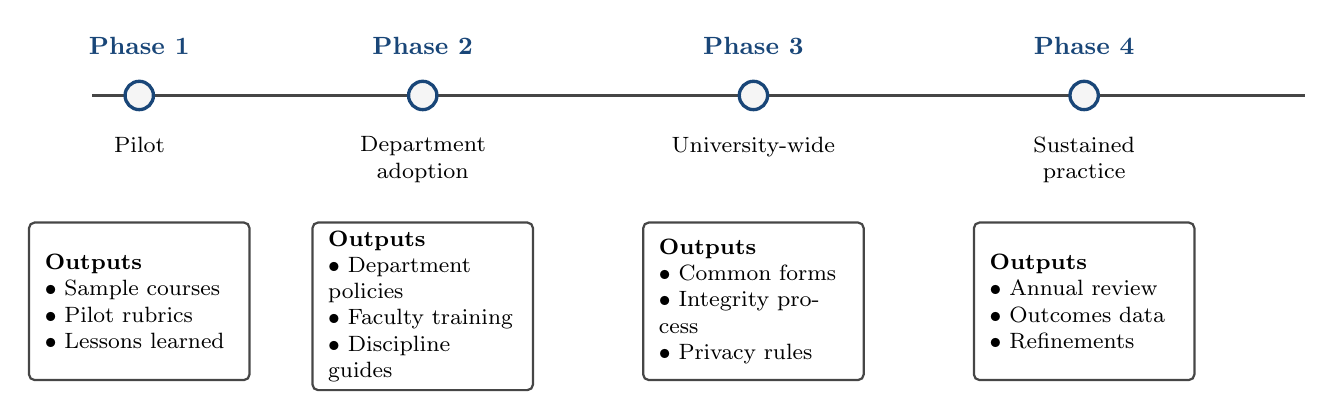
\begin{tikzpicture}[node distance=0.4cm and 0.4cm, every node/.style={font=\small}]
% Timeline base line
\draw[very thick, draw=darkgray] (0, 0) -- (15.4, 0);

% Four phase markers
\foreach \x/\name/\desc in {
  0.6/{Phase 1}/{Pilot},
  4.2/{Phase 2}/{Department\\adoption},
  8.4/{Phase 3}/{University-wide},
  12.6/{Phase 4}/{Sustained\\practice}}
{
  \filldraw[draw=guideblue, fill=lightgray, very thick] (\x, 0) circle (0.18);
  \node[font=\small\bfseries, color=guideblue, above=0.4cm of {(\x, 0)}] {\name};
  \node[font=\footnotesize, align=center, below=0.4cm of {(\x, 0)}, text width=2.6cm] {\desc};
}

% Deliverables under each phase
\node[secondary-node, below=1.6cm of {(0.6, 0)}, minimum width=2.8cm, minimum height=2.0cm, align=left, text width=2.4cm]
  {\footnotesize\textbf{Outputs}\\
   \footnotesize $\bullet$ Sample courses\\
   \footnotesize $\bullet$ Pilot rubrics\\
   \footnotesize $\bullet$ Lessons learned};
\node[secondary-node, below=1.6cm of {(4.2, 0)}, minimum width=2.8cm, minimum height=2.0cm, align=left, text width=2.4cm]
  {\footnotesize\textbf{Outputs}\\
   \footnotesize $\bullet$ Department\\policies\\
   \footnotesize $\bullet$ Faculty training\\
   \footnotesize $\bullet$ Discipline guides};
\node[secondary-node, below=1.6cm of {(8.4, 0)}, minimum width=2.8cm, minimum height=2.0cm, align=left, text width=2.4cm]
  {\footnotesize\textbf{Outputs}\\
   \footnotesize $\bullet$ Common forms\\
   \footnotesize $\bullet$ Integrity process\\
   \footnotesize $\bullet$ Privacy rules};
\node[secondary-node, below=1.6cm of {(12.6, 0)}, minimum width=2.8cm, minimum height=2.0cm, align=left, text width=2.4cm]
  {\footnotesize\textbf{Outputs}\\
   \footnotesize $\bullet$ Annual review\\
   \footnotesize $\bullet$ Outcomes data\\
   \footnotesize $\bullet$ Refinements};
\end{tikzpicture}}%
\caption{\textbf{Four-phase implementation timeline.} Universities adopt the framework progressively rather than at once. Phase~1 builds confidence in a small set of courses; Phase~2 lets departments localize; Phase~3 creates institutional consistency; Phase~4 maintains and refines. Each phase produces concrete outputs that feed the next.}
\label{fig:implementation-timeline}
\end{figure}

\subsection{Phase 1: Pilot}
\label{u:subsec:pilot}

Select a small set of courses across disciplines and sizes. Include at least one large undergraduate course, one writing-intensive course, one STEM course, and one seminar or capstone. Test the shared vocabulary, assignment labels, disclosure form, and assessment models.

Collect feedback from students, instructors, TAs, and academic-integrity staff. Revise the materials before wider adoption.

\subsection{Phase 2: Department adoption}
\label{u:subsec:department-adoption}

Departments adapt the framework to local needs. They identify core competence standards, discipline-specific verification practices, sample assignments, and course-size models. They also decide which courses should include explicit AI literacy outcomes. \Cref{u:app:department-checklist} lists what a department needs in place before it starts.

\subsection{Phase 3: University adoption}
\label{u:subsec:university-adoption}

The university integrates the framework into syllabus guidance, teaching-center resources, student orientation, academic-integrity procedures, and data-governance policy. The policy should remain flexible enough for local course design.

\subsection{Phase 4: Review and revision}
\label{u:subsec:review-revision}

AI policy should be reviewed annually. The review should examine student learning, faculty workload, integrity cases, equity concerns, privacy incidents, and student feedback. Review should be scheduled, not only triggered by problems. Beyond the institutional cycle, instructors should revisit their course-level AI policy each time they teach the course, since both the tools and students' familiarity with them shift from term to term. The goal is not permanent policy language. The goal is stable principles with adaptable implementation.

\subsection{Cost and resource considerations}
\label{u:subsec:cost-considerations}%
\index{stipends}%
\index{implementation plan!cost}

The four-phase plan above describes what to do but not what it costs. Honest implementation discussion has to acknowledge that AI-aware teaching is a real institutional investment. Disclosure-protocol design and faculty workshops in Phase 1 typically require teaching-center staff time and a modest stipend pool for pilot instructors. Process-evidence rubrics in Phase 2 increase per-assignment grading time, which means departments with high enrollment-to-instructor ratios may need to reallocate teaching assistant support or accept somewhat coarser rubrics. Oral assessment, the most future-proof element of the framework, is the most expensive to scale; small classes can absorb it within existing contact hours, while large classes typically cannot without TA support or a hybrid in-class/recorded model. Calibration sessions across instructors are the lowest-cost element on a per-session basis but require persistent scheduling investment that departments often underestimate.

For resource-constrained departments, a useful adoption path is to begin with three low-cash-cost elements that do not require new hiring: explicit per-assignment AI policies; the disclosure-block standard, largely a one-time setup; and a single calibration session per term. These cost little new money, but each costs faculty time, which is neither free nor abundant. The path shifts cost from the budget line to the workload, and a chair or dean should plan for that workload rather than assume it away. What the time and the money buy is the validity of the credential: assessment that still certifies what a graduate can do. The full framework can then be phased in over multiple years as resources allow. The goal of the implementation plan is not to require simultaneous adoption of every element, but to give departments a coherent target state to grow toward.

For institutions in UNESCO-aligned policy environments, the CAT-to-UNESCO crosswalks established earlier in this volume (Tables~\ref{tab:cat-unesco} and~\ref{tab:instructor-unesco}, and the learning-outcomes mapping in \cref{u:subsec:unesco-outcomes}) can be used directly during accreditation reporting, curriculum-revision proposals, and international-collaboration framing. Where the institution's accreditation language references UNESCO student or teacher AI competence frameworks, the crosswalks make the alignment explicit and reduce the translation work for adopting departments. National-policy environments outside UNESCO alignment can perform analogous mappings against their own framework documents; the CAT structure is intended to translate cleanly onto most national or regional frameworks rather than to compete with them \citep{usde2023artificial}.

\section{Faculty change management}
\label{u:sec:change-management}%
\index{faculty development!change management}

The framework laid out in the previous sections describes what an institution should do. It does not describe how a university actually moves from current practice to that target state. The gap between the two is faculty change management, and it is where most well-designed AI policies fail.

The guidance here draws on practical experience with faculty adoption and on the higher-education change-management literature, an established empirical body that predates AI but bears directly on the problem. Analytic reviews of how faculty adopt new teaching practices find that top-down administrator mandates and the dissemination of model curricula are, on their own, largely ineffective, and that durable change instead depends on sustained support, local evidence, and faculty engagement \citep{henderson2011facilitating,borrego2014increasing,kezar2013colleges}. What remains AI-specific, and is still accumulating, is direct evidence on this framework's particular elements. The guidance below is therefore offered as informed practice grounded in that broader literature, rather than as the kind of settled AI-specific finding that anchors much of Parts~\ref{part:student} and~\ref{part:instructor}.

\subsection{The change-management problem}
\label{u:subsec:change-problem}

Faculty are not, in general, opposed to AI policy in principle. Most instructors recognize that AI tools have changed what students bring to class and what assignments measure. The resistance an institution encounters is rarely ideological. It is practical. New disclosure conventions add a small amount of work to every assignment. Process-evidence rubrics take longer to grade. Oral assessments require time many faculty do not have. Calibration sessions across instructors require coordination that departments are not staffed to provide.

A faculty member who is already teaching three courses, advising graduate students, serving on two committees, and writing a tenure file does not need a new burden. The honest framing is that AI-aware teaching is real additional work, at least at first, and institutional change management has to start from that recognition.

A second source of resistance is worth naming. Some faculty believe their existing practice already addresses AI use adequately. They may be right; some courses are naturally AI-resistant by design. They may also be wrong, and the wrong cases tend to surface only when a student fails an oral audit or when a graduate program discovers a thesis chapter cannot be defended. The change-management challenge is to provide enough scaffolding that even faculty who do not see the problem can adopt practices that protect them and their students if it appears.

\subsection{Stages of faculty adoption}
\label{u:subsec:adoption-stages}%
\index{buy-in, faculty}%
\index{faculty development!attendance}

Faculty distribute across at least four broad groups, each requiring a different kind of support. The grouping draws loosely on the diffusion-of-innovations literature, which has consistently identified distinct adopter categories with characteristic motivations and barriers \citep{rogers2003diffusion}. The labels matter less than the recognition that one approach will not reach all groups.

\textit{Skeptics} doubt that AI policy is needed at all in their course. They may believe their existing safeguards (in-person exams, oral components, structured drafts) already prevent the failure modes the policy targets. The most useful intervention is not advocacy but evidence: invite skeptics to participate in calibration sessions where they grade student submissions blind alongside other instructors. The conversations that follow are usually more persuasive than any presentation.

\textit{Pragmatists} will adopt new practices if shown clear benefit and if the marginal workload is manageable. They want concrete templates, sample rubrics, and ready-made assignment redesigns rather than principles. The most useful intervention is shared resources: a department-level library of AI-aware assignments organized by course type, a small set of validated rubrics, and one or two paragraphs of standard syllabus language. Pragmatists are the largest group on most faculties; the framework's adoption depends on them.

\textit{Early adopters} are already running ahead of policy. Some have been redesigning assignments for two years; some have published their experiments. Their needs are different: they want recognition, the chance to influence institutional direction, and protection against being penalized for trying. The most useful intervention is to involve them in policy design and to let them serve as resources for the pragmatist group rather than asking them to attend mandatory training built for skeptics.

\textit{Overwhelmed} faculty\index{contingent faculty!and faculty development}\index{faculty development!faculty paid by the course} want to comply but lack the bandwidth to redesign assignments, learn new tools, or attend additional meetings. They are often contingent faculty, lecturers teaching multiple sections, or faculty in caregiving roles. The most useful intervention is reducing the cost of compliance: providing a pre-made syllabus paragraph, a default rubric, and a single accessible workshop rather than a sequence of trainings. For faculty paid by the course, the artifacts have to carry the whole load, because attendance of any kind is time they are not paid for.

A successful adoption strategy reaches all four groups with calibrated support, not all with the same training.

\subsection{Barriers and how to address them}
\label{u:subsec:barriers}%
\index{faculty development!barriers}

Several specific barriers recur across institutions adopting AI-aware teaching.

\textit{Time cost of process-evidence grading.} Reading a draft history, an annotation, and a verification statement takes longer than reading a final submission. The remedy is sampling rather than universal review. A reasonable practice is to grade the final work for everyone and to read process artifacts for a randomly selected subset, plus any submission that raises a concern. Students should be told sampling is in place; this preserves the deterrent effect without the workload of universal audit.

\textit{Lack of confidence in oral assessment.} Many faculty have not conducted structured oral assessments since their own qualifying exams. They worry about consistency, fairness, and student anxiety. The remedy is training that uses real student work, scripts a small set of standard questions, and provides a simple rubric. Most faculty develop confidence after running three or four oral check-ins; the first one is the hardest.

\textit{Concern about fairness to multilingual writers.} Detector-based enforcement is documented to misclassify non-native English writing as AI-generated \citep{liang2023gpt}. Faculty who teach diverse student populations are right to worry about this. The remedy is to abandon detector-only enforcement entirely (\cref{i:sec:integrity}) and to rely on process evidence and student explanation. Faculty who understand this shift in evidentiary standard tend to become advocates for the framework rather than skeptics of it.

\textit{Workload disparities across course sizes.}\index{workload!disparities across course sizes} A 200-student lecture and a 12-person seminar cannot use the same model. Faculty in large courses sometimes feel the framework is designed for small classes and does not address their reality. The remedy is to make the Evidence-of-Thinking Model (\cref{i:sec:evidence-model}) explicit in change-management materials, with concrete examples drawn from large courses.

\textit{Tenure-track and lecturer differences.}\index{release time}\index{contingent faculty!differentiated support} Tenure-track faculty have research obligations that make additional teaching workload genuinely costly to their careers. Contingent faculty and lecturers carry heavier teaching loads and have less time for redesign. Both groups need accommodation, and an institutional approach that ignores these differences will fall hardest on contingent faculty. The remedy is differentiated support: course-release time for redesign work where possible, shared resources that scale across many sections, and recognition that adoption will not look the same across employment categories.

\subsection{When the standard playbook is not enough}
\label{u:subsec:hard-cases}

The four-category adopter model and the barrier remedies above describe what works for most faculty. Departments should also be honest that a small number of faculty will not move regardless of support level. A tenured professor who refuses to use disclosure standards, declines calibration sessions, or actively grades against process-evidence rubrics in their courses can stall department-wide adoption if their courses are gateway requirements for the major. No graceful technical solution to this problem exists. It is a governance problem and should be handled through department governance rather than through additional faculty-development effort.

What works in these cases is usually some combination of four moves. Make the policy a department-level requirement rather than an instructor-level recommendation, so noncompliance becomes a governance issue rather than a matter of personal style. Have course evaluations and curricular reviews ask about AI-policy implementation. Assign a noncompliant faculty member to courses where the policy footprint is smaller, electives rather than gateways. The fourth move is to accept that uniform adoption may take longer than the four-phase plan suggests. Department chairs should not personalize these situations into individual conflict. The goal is institutional adoption, not unanimous instructor agreement, and a small number of holdouts is compatible with effective department-wide practice as long as gateway courses and qualifying milestones are covered.

Institutions should also recognize that a faculty member who appears to be a persistent skeptic may instead be a thoughtful dissenter whose objection is substantive. A serious objection to a particular framework element (for example, that oral assessment as currently implemented produces a particular fairness concern in their student population) may be evidence that the framework needs adaptation rather than that the dissenter needs persuading. Department leadership should distinguish between these cases before treating dissent as obstruction.

\subsection{What works}
\label{u:subsec:what-works}

Several practices recur across institutions that have made meaningful progress.

\textit{Faculty learning communities} that meet regularly to discuss AI in their courses produce more change than any number of workshops. The conversations expose what individual instructors are trying, what is working, and what is not. They also create peer accountability that pure top-down requirements cannot. Five-to-eight faculty meeting monthly is a typical scale.

\textit{Cross-instructor calibration} builds shared standards more effectively than written rubrics alone. Whether faculty exchange one assignment between sections and grade independently, or several instructors grade the same anonymized submission and then discuss, the comparison reveals hidden assumptions about what counts as AI-assisted Practice and resolves them through conversation. The sessions also surface the assessment-validity problems the framework is designed to address (\cref{fig:polished-vs-learning}); faculty often see the polished-output-versus-demonstrated-learning gap clearly when grading a peer's submission. This kind of calibration is rare in higher education but produces large effects when adopted.

\textit{TA training} oriented toward process evidence rather than detector use. Graduate teaching assistants are often the first line of grading in large undergraduate courses; their habits propagate widely. Training should cover the assignment categories (\cref{fig:assignment-color-tree}), the assessment models (\cref{tab:three-models}), and the verification standards (\cref{fig:verification-disciplines}).

\textit{Leadership modeling} by deans, department chairs, and senior faculty matters more than is usually acknowledged. When a department chair publicly redesigns one of their own courses and discusses what worked and what did not, faculty notice. When senior faculty refuse to engage and continue teaching as before, junior faculty hesitate to invest the time in change.

\subsection{What does not work}
\label{u:subsec:what-doesnt-work}

A short list of patterns that institutions try, and that consistently disappoint, deserves explicit naming.

\textit{Mandatory training without local input.} Centrally designed training that does not reflect what nursing instructors, mathematics instructors, and writing instructors actually face produces compliance without change. Faculty attend the session, sign the attendance sheet, and continue teaching as before.

\textit{One-size-fits-all rubrics.} A rubric designed for first-year writing will not work for a graduate proof course. A rubric designed for upper-division engineering will not work for studio art. The framework is intentionally flexible across disciplines (\cref{fig:verification-disciplines}); change-management materials should preserve that flexibility rather than collapsing it.

\textit{Detector-only enforcement.} Using AI-detection scores as the primary basis for academic-integrity action produces false positives, fairness problems for multilingual writers, and erodes trust in faculty judgment \citep{cotton2024chatting}. The teaching-and-learning approach to academic integrity, well-developed before AI tools became prevalent, is more robust \citep{bertramgallant2017academic}. Institutions that rely on detectors create both injustices and litigation risk.

\textit{Discipline-blind requirements.} Mandates that ignore disciplinary differences place a heavier burden on some faculty than others. A mandate to require draft histories on every assignment is sensible for a writing course and unworkable for a calculus course where the assignment is solving twenty problems. Change-management materials should distinguish requirements that apply universally (disclosure, no-detector-only enforcement) from practices that should be adapted by discipline (specific verification protocols, choice of assessment model).

\subsection{Department leadership}
\label{u:subsec:dept-leadership}

The department chair is the most consequential change agent for AI-aware teaching. A dean's policy memo can require new syllabus language; a chair's example shapes daily practice. Three concrete moves are within most chairs' authority.

\textit{A one-page departmental compact} stating what the department expects of every course (clear AI-use rules in syllabi, a defensible Core Competence assessment, disclosure expectations) and what faculty can expect in return (shared rubric library, calibration meeting time, TA training support). The compact should be brief enough to fit on one page and should be revisited annually. A one-page compact outlasts a fifty-page policy manual, because faculty actually read the compact.

\textit{A calibration meeting protocol} held once a semester, where faculty bring one anonymized submission and the group grades it together. The first such meeting feels awkward; subsequent meetings tend to be the most pedagogically valuable hour of the term. Department chairs who model participation in these meetings make them sustainable.

\textit{A teaching-portfolio question for tenure and promotion review.} Adding ``how does the candidate's teaching address responsible AI use'' as one item among many in a teaching dossier signals that the institution treats this as part of teaching rather than as an extra burden. The signal matters more than the assessment; faculty who know this question will be asked tend to take the work seriously.

\subsection{Faculty support resources}
\label{u:subsec:support-resources}

Institutional resources that support faculty change should be visible, accessible, and curated. A short, well-organized set is more useful than a long list of links.

\textit{Teaching center workshops} on AI-aware assignment design, oral assessment, and process-evidence grading. Workshops should be offered both synchronously (with live discussion) and asynchronously (recorded for those who cannot attend). Department-specific sessions, where the workshop draws examples from the participants' own discipline, are consistently more useful than generic sessions. The harder problem is attendance rather than design. A voluntary workshop competes with everything else on a faculty calendar and usually loses, and the faculty who most need it are the least likely to come. Putting the same material on a departmental meeting agenda reaches people no workshop will, and it keeps the disciplinary framing that makes it useful.

\textit{Discipline-specific examples} curated from the disciplinary overlays in Part~\ref{part:instructor}. Faculty in nursing want to see nursing examples; faculty in philosophy want philosophy examples. A small, well-chosen library of example assignments organized by discipline does more work than a large undifferentiated repository.

\textit{Assignment redesign clinics} where a small group of faculty bring an existing assignment, work through one round of redesign with a facilitator, and leave with a revised draft. The format respects faculty time (one session, one assignment) and produces tangible output (a revised assignment they will use). Clinics scale better than one-on-one consultations.

\textit{Shared rubric libraries} organized by assignment category (\cref{fig:assignment-color-tree}) and by assessment model (\cref{tab:three-models}). Rubrics should be lightly curated for quality but not over-standardized. The goal is to give faculty a starting point they can adapt, not to impose uniformity.

These resources become more useful as they accumulate use. A library that contains five well-tested rubrics is more valuable than a library that contains fifty rubrics of unknown quality. Curation is part of the work.

\section[From department to institution]{From department to institution: how departmental practice can shape institutional policy}
\label{u:sec:dept-to-institution}%
\index{departmental practice, shaping policy}

Most readers of this book will not personally drive university-wide AI policy. They will, however, shape what their own department does, and that departmental practice can become the template for what eventually becomes institutional policy. This short section describes how the bridge from department to institution typically works in STEM and adjacent technical settings, and what departmental faculty can do to make that bridge productive rather than frustrating.

\subsection{The pattern in practice}
\label{u:subsec:dept-to-institution-pattern}

Universities rarely adopt comprehensive AI policy in a single top-down decision. Far more often, one or two departments develop coherent practice first, accumulate concrete examples of what works, and become reference cases when university-wide bodies begin to formulate policy. A mathematics department with six semesters of experience with the Oral-Defense Model, three years of disclosure-block practice across all its courses, and a documented academic-integrity procedure is, in effect, handing the institution a tested case study. Similar trajectories work in computer science, statistics, physics, and other quantitative disciplines.

The reverse also holds. When the faculty senate or the academic-integrity committee finally takes up AI policy, it looks for examples of what is already working. Departments that have done the work first are positioned to shape that conversation; departments that have done nothing become subject to whatever the institution decides without their input. Sector data as of 2025 fit this fragmented picture: a large majority of institutions report experimenting with AI, fewer than half have formal governance in place, and most describe their AI strategy as confined to particular units rather than adopted institution-wide \citep{educause2025landscape}. A 2026 mapping of all fifty US flagship public universities sharpens the picture. Every one placed instructional AI decisions at the course level. Institution-level guidance concentrated instead on data protection, approved tools, and risk management \citep{lafrance2026governing}. The departmental layer this Part is built on is the layer that architecture skips, and departments that build coherent practice are filling a gap the sector has left open.

The pattern is consistent with how academic policy typically evolves. Curriculum innovations, assessment innovations, and integrity-policy innovations almost always begin in a single department and spread through demonstration. AI-aware practice is no exception.

\subsection{The college or school in between}
\label{u:subsec:college-layer}%
\index{release time!college-controlled}%
\index{deans}

Department and university are not the only levels. In most universities a college or school sits between them, led by a dean who coordinates several departments, allocates the resources that determine whether AI-aware practice is feasible, and mediates between departmental practice and university policy. The college level is often where the resource decisions in \cref{u:subsec:cost-considerations} are actually made: teaching-assistant lines, teaching-center support, and course-release time for redesign are typically college-controlled. It is also where neighboring departments that share students and standards can align their practice before a university-wide body takes up the question. Departments building AI-aware practice are usually most effective when they bring the college along early, both to secure resources and to position departmental practice as a college-level reference case rather than an isolated experiment.

\subsection{The layer outside the institution}
\label{u:subsec:beyond-institution}%
\index{disciplinary societies}\index{accreditors}

Department, college, and university do not exhaust the possibilities. A 2026 policy forum in \emph{Science}, drawing on original survey data, reaches the same diagnosis this Part begins from and then places the remedy somewhere else. It argues that assessment reform belongs at the level of the discipline, because each discipline carries its own learning goals, assessment traditions, and ways that AI can support or replace student work. The coordinating work, on this account, is best done not by individual universities but by disciplinary societies, accreditors, and other field-level bodies that can write shared guidance and supply examples for local adaptation \citep{chirikov2026generative}.

A discipline is not a department. The two accounts agree that institution-wide policy fails and that the right grain is disciplinary. They disagree about who holds the pen.

The case for the department is that it is the smallest unit with authority over the things that decide whether any of this happens. A society can publish guidance. It cannot run a course, set a syllabus, assign a teaching assistant, or tell a lecturer how to weight an oral defense. Accreditors can require that a program show evidence of learning, and that pressure is real, but the review cycle runs on years while a course runs on weeks. The department hires, schedules, staffs, and reviews. It decides what a shared syllabus says and whether a redesigned course counts toward a colleague's promotion case. Guidance that arrives without those levers becomes another document.

The two placements need not stay rivals. Field-level bodies are well suited to write what a department has neither the time nor the standing to produce alone: model assignments, worked examples, discipline-specific statements of what independent competence means. Departments are suited to adopt, adapt, and enforce them. The society supplies the text and the department supplies the authority. A department waiting for its society to act will wait, and a society writing for departments that have built nothing is writing into a vacuum.

\subsection{What departmental faculty can do to support the bridge}
\label{u:subsec:dept-to-institution-actions}

Faculty whose primary influence is at the department level can still make their work institutionally legible. The most useful actions are:
\begin{enumerate}
\item Document departmental practice in writing, including what was tried, what was kept, and what was discarded, so that the institutional record can refer to it rather than having to reconstruct it.
\item Participate in any institutional working groups, faculty senate committees, or teaching-center conversations that touch AI policy, even briefly, because departmental experience is the missing input these bodies usually lack.
\item Accept invitations to share departmental practice with other departments, which both helps adjacent departments avoid reinventing the wheel and creates the cross-departmental relationships that institutional policy formation depends on.
\item Name the institutional support that would help departmental practice scale, including the Cost and resource considerations from \cref{u:subsec:cost-considerations}, so that institutional policy can be informed by what departments need rather than only by what institutions can mandate.
\end{enumerate}

\subsection{What departments should ask of their institution}
\label{u:subsec:what-to-ask-institution}

Departments doing AI-aware work need a few things from their institution, and institutions are usually willing to provide them once they know to ask:
\begin{itemize}
\item Clear privacy and data-governance policy for AI tool use (so departments do not each have to negotiate licensing separately).
\item A centrally supported pool of AI-tool licenses that gives equity-of-access guarantees so departments do not depend on student personal accounts.
\item An academic-integrity procedure at university level that is compatible with department-level evidence standards (specifically, that does not require detector-tool output as the basis for misconduct decisions, given the documented unreliability described in \cref{u:sec:integrity}).
\item Recognition in the merit-review process, and in hiring and tenure-and-promotion criteria, of the time faculty spend on AI-aware course redesign.
\item A teaching center that can offer the workshop and consultation services described in \cref{u:sec:teaching-center}.
\end{itemize}
Departments that ask for these clearly, in writing, with reference to the framework principles in this volume, are far more likely to receive them than departments that ask for general support without specifics.

\subsection{The honest limit}
\label{u:subsec:honest-limit}

Some institutional decisions are out of departmental hands. Most universities will not adopt the framework here in its entirety; some will adopt fragments; some will adopt nothing and eventually develop their own framework that overlaps imperfectly with this one. Departments should not wait for institutional adoption to do good work in their own courses. The departmental framework is designed to be useful regardless of what the institution does. The institutional framework that follows is offered as guidance for the institutions that wish to use it, not as a precondition for departmental practice. Even in institutions that adopt nothing centrally, a department running coherent practice is providing real value to its students; that value does not depend on whether the policy environment around the department keeps up.

\chapter{Looking Forward}
\label{u:ch:looking-forward}%

\section{Looking forward}
\label{u:sec:looking-forward}%
\index{looking forward}

A framework written in the present moment will encounter capabilities that did not exist when it was written. The volume should acknowledge this honestly without becoming dated. Some predictions about the next several years will be wrong; the framework's structure is designed to remain useful even when specific implementations need refresh.

\subsection{What is likely to change}
\label{u:subsec:will-change}

Several trends seem stable enough to plan around.

AI capability will continue to improve. Recent work on mathematical reasoning suggests that current limitations on proof construction and on multi-step computational reasoning will narrow over the next several years \citep{ahn2024large}. Code generation, multimodal evaluation, and agentic workflows that operate beyond a single chat are all developing faster than university policy cycles.

Tool ubiquity will increase. AI capabilities are moving from separate applications into operating systems, productivity software, and integrated development environments. The distinction between ``using AI'' and ``using a word processor'' will blur, and assignment policies that try to specify which tools count will become harder to maintain. Disclosure-and-verification standards generalize better than tool-by-tool restrictions.

Detector reliability will decrease. As AI-generated text becomes harder to distinguish from competent human writing, the underlying signal that detection tools rely on will weaken. Detectors are already failing in two directions: they produce documented false positives against multilingual writers \citep{liang2023gpt}, and they produce false negatives against students who refine prompts to evoke more literary language. The first direction will increase as detector vendors tune for false-positive control, and the second will increase as student prompting skill becomes ubiquitous. Institutions that built integrity processes around detectors will face mounting reliability problems on both fronts and will need to migrate to the process-based evidence the framework already emphasizes.

Student baseline familiarity will increase. The undergraduates of 2030 will arrive on campus having used AI tools throughout secondary school. Orientation curricula that explain what AI is will become unnecessary; orientation curricula that teach responsible use, verification habits, and disclosure norms will become more important.

\subsection{What is likely to stay the same}
\label{u:subsec:will-stay}

Other elements appear durable across capability shifts.

The need for independent competence will not disappear. A graduate student who cannot reason without tools is not a researcher; a physician who cannot diagnose without AI is not a physician. The specific topics that count as foundational competence may shift, but the underlying requirement that human expertise must extend beyond tool-mediated procedure remains.

Oral assessment will continue to discriminate well between independent understanding and tool-mediated performance, regardless of tool capability. A student who has not built an underlying argument cannot reconstruct it under questioning, and AI capability does not change that. Oral assessment is expensive but durable.

Process evidence will continue to provide signal. The asymmetry between polishing output and developing judgment (\cref{fig:polished-vs-learning}) does not disappear as AI improves. Polish becomes easier; judgment requires the same effort it always did. The competence costume gets cheaper every year; the competence it imitates does not. Assignments that grade process retain validity longer than assignments that grade only final polish.

Disclosure and verification will become more important, not less. As AI involvement becomes ubiquitous and harder to detect, the burden shifts from external detection to internal disclosure. Verification standards (\cref{fig:verification-disciplines}) and disclosure norms (Appendix~\ref{app:sciwriting}) protect both the integrity of student work and the trustworthiness of the academic record.

\subsection{What this means for the framework}
\label{u:subsec:framework-stability}

The framework's core elements appear stable across the anticipated changes. The CAT distinction (\cref{sec:cat}) will remain useful regardless of capability shifts because it identifies what an academic course is for, not what a tool can do. The four assignment categories (\cref{fig:assignment-color-tree}) describe the role AI plays in an assignment, which is a curricular choice rather than a tool fact. The three assessment models (\cref{tab:three-models}) reflect course size and staffing constraints that change slowly. The verification standard generalizes across disciplines and across tool generations.

What will need refresh is the specific content within those structures. Tool lists will need annual updates. Prompt examples will date quickly; the prompt examples in Part~\ref{part:student} are illustrative rather than canonical. Disclosure templates will evolve as institutional norms develop. Detector references should be removed from policy documents wherever they appear; this volume already takes that position, but many existing institutional policies have not.

The recommendation for departments adopting the framework is to plan annual reviews of implementation specifics (tools, prompts, templates) on a stable foundation of structural commitments (categories, models, verification, disclosure). Annual reviews are part of Phase 4 (\cref{u:subsec:review-revision}); the change-management chapter argues that those reviews are also faculty change-management opportunities.

\subsection{Why this is hard, and where the levers are}
\label{u:subsec:leverage}

Before the book closes, one thing is worth saying plainly. Everything in this book asks students, instructors, and institutions to choose the harder path exactly where the easier one is cheaper and its damage is hidden. The metacognitive gap hides the learning loss, so no one feels the cost of skipping the judgment work. Enrollment pressure and faculty workload reward the shortcut. The framework runs against that gradient, and naming the trilemma does not flatten it.

Two levers change the slope. The first is no-AI assessment. Its value is not only that it is much harder to game. It makes the learning loss visible, and a loss you can measure is a loss an institution can act on. The second is setting integrity standards centrally, decoupled from enrollment incentives, so that no single course or department pays alone for holding the line. Without them, the honest prediction is that the framework is adopted by the conscientious and skipped by the pressured. That would reproduce at scale the very split the trilemma describes: diligent against strategic, resourced against time-poor. With them, the gradient no longer runs against the unit that holds the line. That alignment, not exhortation, is what turns a framework into practice.

\subsection{Modesty about prediction}
\label{u:subsec:modesty}

Specific predictions will be wrong. Some capabilities anticipated above will arrive faster than expected; others will plateau. Some failure modes will be solved; others will appear that no one currently anticipates. The framework is designed to be more durable than any specific tool list, but it is not designed to be permanent. Universities adopting it should expect to revise the implementation details every year and the structural commitments every five years or so.

A useful posture is to treat this volume as a working document rather than a settled answer. Departments that find the framework helpful are encouraged to adapt it, document their adaptations, and share what they learn. The framework improves by use, not by being right in advance.

This returns to where the book began. The camera, the calculator, and the power tool did not remove the practitioner; each moved the work up a level, from execution to judgment. A university adopting this framework is making that move deliberately, deciding while the tools are still new what the higher level of work requires and how to teach it.

\section{Adoption claims and metrics}
\label{u:sec:metrics}%
\index{evaluation metrics}\index{evidence status}

Before adopting a framework, an administrator should know what it rests on. The book states its
evidentiary limits where each claim is made. Gathered in one place, they look like this.

\begin{longtable}{>{\raggedright\arraybackslash}p{0.30\textwidth}>{\raggedright\arraybackslash}p{0.34\textwidth}>{\raggedright\arraybackslash}p{0.26\textwidth}}
  \caption{What the framework rests on.}\label{u:tab:evidence-status}\\
  \toprule
  Claim & What supports it & Status \\
  \midrule
  \endfirsthead
  \toprule
  Claim & What supports it & Status \\
  \midrule
  \endhead
  AI writes fluently and can be confidently wrong, including inventing sources. & Published research on language-model behavior \citep{bender2021dangers,walters2023fabrication}. & Established. \\
  Unrestricted AI use can raise short-term output while weakening durable understanding, and students do not notice the loss. & A field experiment with a control group \citep{bastani2025generative}. & Established. \\
  Detector-based enforcement is unreliable and falls unevenly across students. & Published evaluation of detector performance \citep{liang2023gpt}. & Established. \\
  Careful design can make AI genuinely useful for learning. & A randomized comparison in a physics course \citep{kestin2025ai}. & Established. \\
  Institutional adoption has outrun institutional policy. & Survey of faculty governance \citep{aaup2025artificial}. & Established. \\
  Redesigning assessment around independent competence checks and oral defense removes the advantage of skipping the work. & One course redesigned this way, where students with and without AI reached similar outcomes \citep{kosar2024computer}. & Closest direct evidence. Tests the style of redesign, not this framework. \\
  Departments are the layer where AI policy should be set. & Documented delegation from institution to course across fifty flagship universities \citep{lafrance2026governing}. A \emph{Science} policy forum agrees the layer is skipped and places the remedy outside the institution, with disciplinary societies and accreditors \citep{chirikov2026generative}. & Contested. The gap is documented from both sides. Neither placement is tested. \\
  The four assignment categories make expectations clearer to state and easier to follow. & Reasoning from the rows above. & Untested. \\
  The three assessment models yield more trustworthy evidence of learning. & Partial, through the redesign above. & Untested as a set. \\
  Courses built on this framework produce better learning than courses that are not. & Nothing. No study has asked. & Untested. \\
  \bottomrule
\end{longtable}

The last three rows are the honest ones. They are also the reason for what follows. A department that
runs the framework and measures what happens becomes the study the last row is waiting for.

\subsection{Metrics}

A university should evaluate whether the framework improves learning and fairness. Useful metrics
include:

\begin{itemize}
  \item percentage of syllabi with clear AI-use rules;
  \item percentage of courses identifying independent competence assessments;
  \item student understanding of AI disclosure expectations;
  \item faculty confidence in AI-aware assignment design;
  \item TA grading consistency on process-evidence rubrics;
  \item student performance on no-AI transfer checks;
  \item quality of student verification statements;
  \item number and type of academic-integrity cases;
  \item frequency of detector-only misconduct claims;
  \item student reports of fairness, access, and privacy clarity;
  \item adoption of approved tools rather than unsupported tools;
  \item faculty workload effects.
\end{itemize}

The purpose of measurement is improvement. If students disclose AI use but cannot verify claims, the student training needs revision. If faculty avoid AI assignments because grading process evidence is too burdensome, the institution should provide better rubrics or TA support. If large courses rely mainly on polished take-home work, assessment validity may need attention.

\subsection{A self-study a department can run}
\label{u:subsec:self-study}%
\index{self-study protocol}

Those metrics answer whether a department is improving. With four additions they answer something
larger, which is whether the framework works at all.

Measure before you adopt. A department that starts measuring after the change has nothing to compare
against, and one term of baseline is worth more than three terms of after.

Leave some sections alone at first. Where a course runs several sections, stagger adoption by a term.
The unchanged sections are not a control group in the strict sense, since instructors differ, but the
comparison is far better than none.

Watch the transfer checks most closely. Syllabus counts and faculty confidence are easy to move and
tell you little. How students do without AI, on material they were taught with it, is the measure
that speaks to learning, and the one the literature lacks.

Write down what you find, including the parts that did not work. Departments that publish a plain
account of two years of adoption, with numbers, will settle questions this book can only reason
about. Nothing here requires a grant or an education researcher. It requires a baseline, a
comparison, and the willingness to report a result that was not the one hoped for.

\section{Risk register}
\label{u:sec:risk-register}%
\index{risk register}

Institutional adoption should include a simple risk register.

\begin{longtable}{>{\raggedright\arraybackslash}p{0.24\textwidth}>{\raggedright\arraybackslash}p{0.34\textwidth}>{\raggedright\arraybackslash}p{0.32\textwidth}}
  \caption{Common risks and institutional responses.}\label{u:tab:risk-register}\\
  \toprule
  Risk & Why it matters & Recommended response \\
  \midrule
  \endfirsthead
  \toprule
  Risk & Why it matters & Recommended response \\
  \midrule
  \endhead
  Over-reliance on AI & Habitual first-resort AI use erodes the independent skill the course is meant to build, even when each single use looks harmless. & Require independent competence checks and evidence-of-thinking assignments. \\
  Detector dependence & Detection tools may be unreliable and unfair. & Use process evidence, student explanation, and due process. \\
  Privacy breaches & Students or faculty may upload protected data. & Maintain approved-tool lists and clear no-upload rules. \\
  Unequal access & Paid tools can create academic advantage, and procurement can create it too: license tiers that differ across units, and pilots that expire mid-semester and strand the students inside them. & Provide institutionally supported tools or equivalent alternatives; match tiers across sections, and let no pilot end mid-term. \\
  Faculty workload & Process grading and audits can add burden. & Provide templates, TA calibration, sampling methods, and reusable rubrics. \\
  Core Competence narrowing & Independent competence checks are costly to run, so a department gradually keeps the competences that fit an oral slot or a class period and drops the ones that do not. Outcome metrics stay healthy throughout, because students still perform on what is asked. & At scheduled review, compare the Core Competence definition against the one written at adoption, and record what left the list and why. \\
Policy fragmentation & Students receive conflicting rules across courses. & Use shared vocabulary and assignment categories while preserving local flexibility. \\
  False confidence & Fluent AI output leads students to overestimate what they understand; self-assessment fails to track the deficit. & Include transfer checks, oral explanations, and audit-and-repair tasks. \\
  Underuse of AI literacy & Students may be told what not to do without being taught what to do. & Include explicit student training and AIS assignments. \\
  Budget-model incentives & Under enrollment-linked budgeting such as RCM, units that allow broader AI use may draw students from stricter units, pressuring all units toward leniency. & Set core AI-integrity expectations institutionally so units do not compete on permissiveness; keep integrity standards decoupled from unit-level enrollment incentives. \\
  \bottomrule
\end{longtable}



\section{Model institutional policy statement}
\label{u:sec:model-policy}%
\index{model institutional policy statement}

The following language can be adapted for a university policy page.

\begin{quote}
The university recognizes that artificial intelligence tools are now part of academic, professional, and creative work. Students should learn to use these tools responsibly while continuing to develop the independent knowledge, skills, and judgment that each course requires.

Each course must state how AI may or may not be used. Instructors should identify which assignments prohibit AI, which allow AI for tutoring or study support, which allow AI as a collaborator, and which ask students to analyze AI directly. Students are responsible for following course rules, verifying AI-assisted work, protecting private or restricted information, and disclosing AI use when required.

Instructors remain responsible for grading, feedback, and academic-integrity judgments. AI tools may assist instruction, but they should not replace human evaluation. Suspected misuse should be handled through process evidence, student explanation, and established academic-integrity procedures. AI-detector scores should not be used as the sole or primary evidence of misconduct.
\end{quote}

\section{Evidence base and limits}
\label{u:sec:evidence-limits}

Institutional AI policy is developing faster than the research base. The shared evidence summarized in \cref{sec:evidence-limits} of Part~\ref{part:student} establishes the learning-science foundation that AI-aware policy must preserve. For institutions specifically, two additional findings are stable enough to guide practice: automated text detectors are not reliable enough to serve as the sole basis for misconduct decisions, and AI tools raise privacy, access, and equity concerns that universities must address directly. A 2026 systematic review of institutional generative AI governance reaches compatible conclusions \citep{bacalso2026institutional}. It calls for embedded governance, equity safeguards, sustained faculty development, and continuous monitoring.

A third stable finding worth naming at the institutional level is the \emph{performance-versus-learning gap}. The OECD's 2026 Digital Education Outlook frames the central evidentiary problem as follows: generative AI tools may enhance the apparent quality of student work (its performance at educational tasks) without improving actual learning, the durable knowledge and skill acquisition the work was supposed to demonstrate \citep{oecd2026digital}. Multiple studies converge on this distinction. Institutions that evaluate the success of their AI policies primarily by submitted-artifact quality will systematically miss this gap; institutions that evaluate success by post-AI independent performance, oral-defense outcomes, or transfer-question accuracy will catch it. The implementation plan in this Part is designed to surface the gap rather than mask it; the assessment models and rubrics in Part~\ref{part:instructor} are the operational tools.

Other questions remain unsettled. The best balance between no-AI, bounded-AI, and open-AI assessment will vary by field, level, and class size. AI tools will also change. For that reason, this framework should be adopted as a living policy. It gives institutions a shared starting point, not a final answer.

\section{Reference materials}
\label{u:sec:part3-refs}

The following worksheets, templates, and checklists support institutional adoption of the framework. Each may be adapted for local use; the items are designed to be lifted into faculty-handbook material, syllabus-design guidance, or chair-level operations documents. Global technical references (GMIP, M/A/E framework, scientific writing) appear at the end of the volume.

\subsection{Course classification worksheet}
\label{u:app:course-classification}

Instructors or departments can use this worksheet before the semester begins.

\begin{enumerate}
  \item What are the three to five core abilities students must develop in this course?
  \item Which of those abilities must students demonstrate without AI?
  \item Which assignments are NAI, AIT, AIC, or AIS?
  \item What evidence will show that students understand submitted work?
  \item Is the course best suited to the Oral-Defense Model, Evidence-of-Thinking Model, or Hybrid Model?
  \item What privacy restrictions are most relevant to this course?
  \item What disclosure format will students use?
  \item What student training is needed before the first AI-permitted assignment?
  \item What grading support or TA calibration is needed?
  \item How will the course be evaluated and revised after the term?
\end{enumerate}

\subsection{Syllabus template}
\label{u:app:syllabus-template}

\subsection*{AI use in this course}

This course uses the following AI-use categories.

\begin{description}
  \item[NAI assignments.] AI use is not allowed. These assignments assess what you can do independently.
  \item[AIT assignments.] AI may be used for study support, explanation, practice, and hints, but not to produce submitted work.
  \item[AIC assignments.] AI may be used as a collaborator for brainstorming, revision, debugging, critique, or testing. You must verify the work and disclose your use.
  \item[AIS assignments.] AI is part of the object of study. You may be asked to analyze, critique, compare, or repair AI output.
\end{description}

For any assignment that permits AI, your submission must follow the disclosure instructions given with the assignment. You are responsible for all submitted work. You should not submit AI output that you cannot explain, verify, or defend.

Do not upload private, restricted, copyrighted, confidential, clinical, human-subject, or secure assessment material into AI systems unless the instructor has explicitly approved that use.

\subsection{Disclosure block}
\label{u:app:disclosure-block}

\begin{quote}
\textbf{Tools used:} Name the tools used, if any.\\
\textbf{Tool role:} Describe what the tools helped with.\\
\textbf{Student role:} Describe what you wrote, revised, checked, or decided.\\
\textbf{Accepted, changed, or rejected:} Describe the AI contributions you used, revised, or set aside.\\
\textbf{Independent verification:} Describe how you checked important claims, sources, data, code, or reasoning.\\
\textbf{What I can explain without AI:} Name the main parts of the work you can now explain on your own.
\end{quote}

\subsection{Privacy checklist}
\label{u:app:privacy-checklist}

Before using AI in a course, ask:

\begin{enumerate}
  \item Is the tool approved for this type of use?
  \item Does the task involve student records, grades, private communications, clinical data, research-subject data, or confidential material?
  \item Could student work be stored, reused, or used for training by the vendor?
  \item Are students required to create personal accounts?
  \item Is there a no-cost option or equivalent alternative?
  \item Is the tool accessible to students with disabilities?
  \item Are students told what not to upload?
  \item Has the instructor provided a privacy-safe alternative when needed?
\end{enumerate}

\subsection{Academic-integrity workflow}
\label{u:app:integrity-workflow}

When AI misuse is suspected, instructors should avoid beginning with accusation. A fair workflow is:

\begin{enumerate}
  \item Re-read the assignment's AI-use rule.
  \item Gather available evidence, including process evidence and comparison to other course work.
  \item Invite the student to explain the work.
  \item Ask targeted questions about sources, reasoning, method, code, data, or revision choices.
  \item If needed, assign a short reassessment tied to the submitted work.
  \item Decide whether the issue is misunderstanding, poor documentation, prohibited assistance, or deliberate misrepresentation.
  \item Apply the appropriate educational or formal response under institutional policy.
\end{enumerate}

\subsection{Department adoption checklist}
\label{u:app:department-checklist}

A department is ready for adoption when it has:

\begin{itemize}
  \item approved shared AI-use vocabulary;
  \item provided sample syllabus language;
  \item identified discipline-specific verification practices;
  \item developed examples of NAI, AIT, AIC, and AIS assignments;
  \item stated expectations for independent competence;
  \item provided a disclosure template;
  \item created a process for large-course TA calibration;
  \item clarified privacy and tool-use rules;
  \item aligned academic-integrity procedures with the institutional framework;
  \item scheduled periodic review.
\end{itemize}

\index{departmental adoption kit}\index{policy self-audit}Two companion files carry the list further. The departmental adoption kit (\texttt{institutions/department-adoption-kit.md}) turns it into a day-one toolset for a chair, with a model policy statement, the shared vocabulary, the four assignment categories, and a one-semester rollout. The policy self-audit (\texttt{institutions/policy-self-audit.md}) runs thirty-two checks across six dimensions. It separates what the institution already covers from what the department covers, and from what neither one does.

\subsection{Program evaluation rubric}
\label{u:app:evaluation-rubric}

A university can evaluate implementation using the five-level rubric in \cref{u:tab:implementation-rubric}.

\begin{longtable}{>{\raggedright\arraybackslash}p{0.22\textwidth}>{\raggedright\arraybackslash}p{0.68\textwidth}}
  \caption{Institutional implementation rubric.}\label{u:tab:implementation-rubric}\\
  \toprule
  Level & Description \\
  \midrule
  \endfirsthead
  \toprule
  Level & Description \\
  \midrule
  \endhead
  1. Fragmented & AI policies vary widely, many syllabi are unclear, and faculty have few shared resources. \\
  2. Emerging & Some departments use clear policies, but vocabulary, privacy rules, and assessment models are inconsistent. \\
  3. Functional & Most courses state AI-use rules, and the institution provides basic templates, training, and academic-integrity guidance. \\
  4. Mature & Departments use shared vocabulary, course-size models, disclosure standards, privacy safeguards, and calibrated assessment practices. \\
  5. Exemplary & AI literacy, independent competence, responsible judgment, equity, privacy, and assessment validity are integrated into regular course design and program review. \\
  \bottomrule
\end{longtable}

\subsection{One-page adoption summary}
\label{u:app:one-page-summary}%
\index{adoption summary, one-page}

The institutional framework can be summarized in ten commitments.

\begin{enumerate}
  \item Teach students to use AI without surrendering their own thinking.
  \item Require every course to state its AI-use rules.
  \item Preserve meaningful assessment of independent competence.
  \item Treat AI literacy as an educational outcome.
  \item Require verification of AI-assisted work.
  \item Normalize brief, factual disclosure.
  \item Protect privacy, access, and equity.
  \item Avoid detector-only misconduct decisions.
  \item Support faculty with templates, training, and TA calibration.
  \item Review policies regularly as tools and practices change.
\end{enumerate}

% ============================================================================
% APPENDICES
% ============================================================================

\appendix

% ============================================================================
% APPENDIX A - Graduate Mathematical Intelligence Profile (GMIP)
% ============================================================================

\chapter{Graduate Mathematical Intelligence Profile}
\label{app:ch:graduate-mathematical-intelligence-profile}%
\label{app:gmip}

\bookepigraph{Two transcripts.\\One records what the student can prove.\\The other records what they can responsibly verify.}

This appendix presents the \emph{Graduate Mathematical Intelligence Profile} (GMIP), the source framework from which the CAT framework in this book is generalized. GMIP was developed for graduate mathematics departments that expect students to use AI tools as part of serious mathematical work. It is presented here in technical-reference form for departments and instructors who want to adopt or adapt it directly.

GMIP separates what departments want students to become from what tools can produce on their behalf. It treats graduate mathematical ability as a profile of stable competencies, each of which can be assessed under different tool conditions. The framework is intentionally conservative about claims and grading. It assumes that AI models will continue to improve, and it therefore prioritizes assessments that require mathematical judgment, verification habits, coherent reasoning under questioning, and ethical disclosure of tool use.

\section{Two-transcript design}
\label{app:gmip-transcripts}%
\index{GMIP}\index{GMIP!two-transcript design}\index{Mathematics Transcript}\index{AI-Integrated Transcript}

GMIP organizes evaluation into two linked transcripts (\cref{fig:two-transcripts}).

\begin{description}
\item[Mathematics Transcript.] What the student can do with no assistance or with limited assistance. Primary instruments are no-AI written exams, oral examinations at the blackboard, and short proof or concept tasks under closed-resource conditions.

\item[AI-Integrated Transcript.] What the student can do when using tools responsibly to accelerate and deepen mathematical work. Primary instruments are open-tool homework with process artifacts, AI-critique and error-detection tasks, comparative human--AI problem solving, and AI-assisted research projects.
\end{description}

\begin{figure}[ht]
\centering
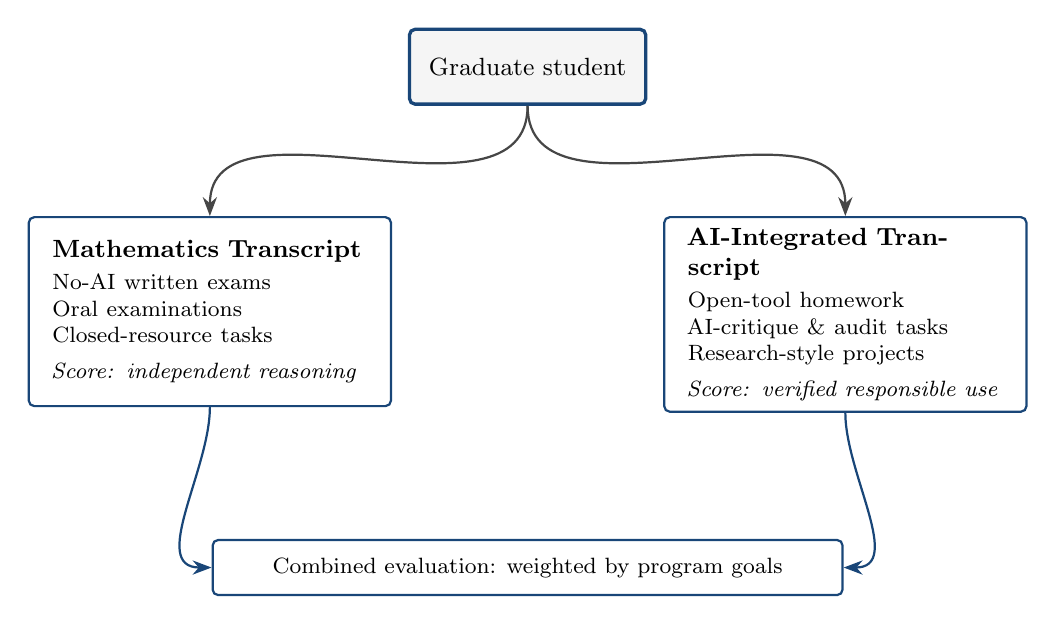
\begin{tikzpicture}[node distance=0.6cm and 1.2cm]
% Student node at top
\node[emphasis-node, minimum width=3cm] (student) {Graduate student};

% Two transcript boxes
\node[framework-node, below left=1.4cm and 0.2cm of student, minimum width=4.6cm, minimum height=2.4cm, align=left, text width=4.0cm] (math)
  {\textbf{Mathematics Transcript}\\[2pt]
   \footnotesize No-AI written exams\\
   \footnotesize Oral examinations\\
   \footnotesize Closed-resource tasks\\[2pt]
   \footnotesize \textit{Score: independent reasoning}};

\node[framework-node, below right=1.4cm and 0.2cm of student, minimum width=4.6cm, minimum height=2.4cm, align=left, text width=4.0cm] (ai)
  {\textbf{AI-Integrated Transcript}\\[2pt]
   \footnotesize Open-tool homework\\
   \footnotesize AI-critique \& audit tasks\\
   \footnotesize Research-style projects\\[2pt]
   \footnotesize \textit{Score: verified responsible use}};

% Arrows from student down to each transcript
\draw[flow-arrow] (student.south) to[out=-90, in=90] (math.north);
\draw[flow-arrow] (student.south) to[out=-90, in=90] (ai.north);

% Combined assessment label below
\node[secondary-node, below=5.5cm of student, minimum width=8cm, minimum height=0.7cm, draw=guideblue] (combined)
  {Combined evaluation: weighted by program goals};

% Arrows from each transcript down to combined
\draw[flow-arrow, draw=guideblue] (math.south) to[out=-90, in=180] (combined.west);
\draw[flow-arrow, draw=guideblue] (ai.south) to[out=-90, in=0] (combined.east);
\end{tikzpicture}
\caption{\textbf{The two-transcript design.} Each graduate student's mathematical record is split into two parallel transcripts. The Mathematics Transcript captures what the student can do independently; the AI-Integrated Transcript captures what the student can do with AI tools used responsibly. Neither alone is sufficient.}
\label{fig:two-transcripts}
\end{figure}

A grade can be computed from these transcripts, but the larger goal is diagnostic: GMIP is designed to tell a student and their advisor what kind of mathematician the student is becoming and what to strengthen next.

\section{Five core design principles}

GMIP rests on five design principles that distinguish it from conventional mathematical assessment.

\begin{enumerate}
\item \textbf{Tool-conditional assessment.} Evaluate the same competency in multiple tool regimes (no-AI, bounded-AI, open-AI). The same student may show strength in one regime and weakness in another, and that pattern is itself diagnostic.

\item \textbf{Evidence-first grading.} Require artifacts that make reasoning inspectable: scratch work, proof sketches, checklists, verification logs. A correct final answer does not establish mathematical understanding if no reasoning evidence is visible.

\item \textbf{Verification over fluency.} Reward students who can detect and repair errors, including errors produced by tools. AI models can generate fluent mathematics that contains subtle flaws. The student who notices and fixes those flaws is demonstrating exactly the skill the discipline values.

\item \textbf{Process integrity.} Require transparent disclosure of tool usage and enforce clear boundaries on what counts as the student's own contribution. The boundaries should be stated in writing, applied consistently across courses, and discussed openly with students.

\item \textbf{Oral grounding.} Reserve a meaningful portion of the grade for live reasoning, where understanding is hardest to outsource. Oral examinations are among the most durable assessments because they probe the present-tense thinking of the student in front of the examiner.
\end{enumerate}

\section{The eight competency domains}

GMIP evaluates graduate mathematical intelligence through eight competency domains (\cref{fig:gmip-domains}). Departments can adopt all eight or start with a subset. Each domain includes characteristic abilities, observable evidence, and suggested assessments.

\begin{figure}[ht]
\centering
\resizebox{\textwidth}{!}{%
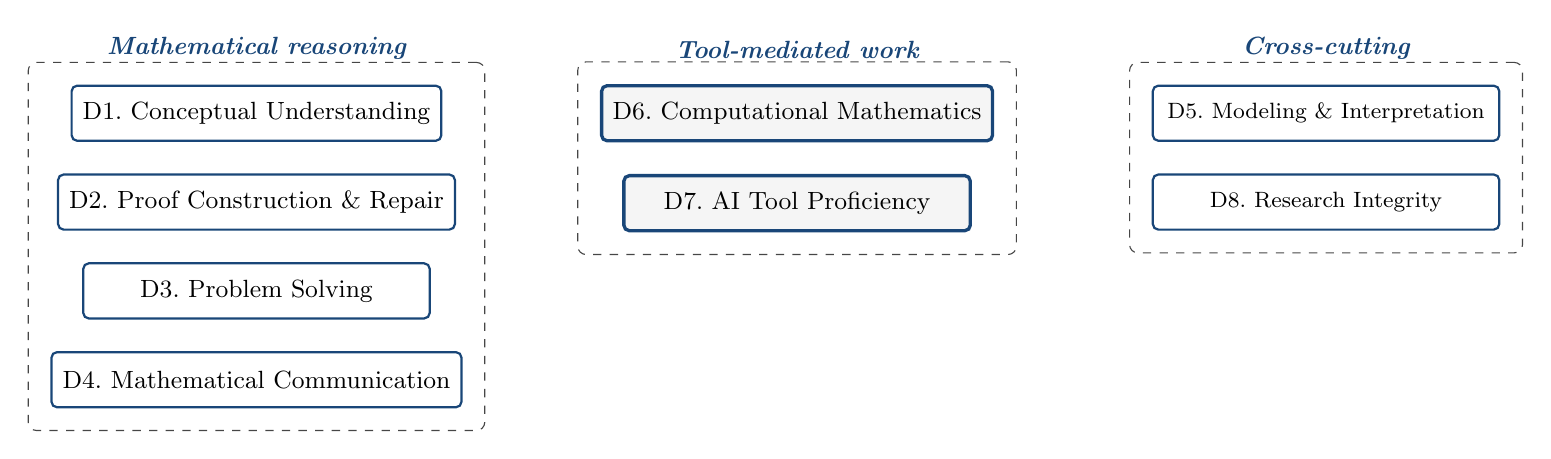
\begin{tikzpicture}[node distance=0.4cm and 0.4cm, every node/.style={font=\footnotesize}]
% Group 1: Pure mathematical reasoning (left column)
\node[framework-node, minimum width=4.4cm, minimum height=0.7cm] (d1) {D1.~Conceptual Understanding};
\node[framework-node, below=of d1, minimum width=4.4cm, minimum height=0.7cm] (d2) {D2.~Proof Construction \& Repair};
\node[framework-node, below=of d2, minimum width=4.4cm, minimum height=0.7cm] (d3) {D3.~Problem Solving};
\node[framework-node, below=of d3, minimum width=4.4cm, minimum height=0.7cm] (d4) {D4.~Mathematical Communication};

\node[font=\small\bfseries\itshape, color=guideblue, above=0.2cm of d1] {Mathematical reasoning};

% Group 2: Tool-mediated work (middle column)
\node[emphasis-node, right=2.0cm of d1, minimum width=4.4cm, minimum height=0.7cm] (d6) {D6.~Computational Mathematics};
\node[emphasis-node, below=of d6, minimum width=4.4cm, minimum height=0.7cm] (d7) {D7.~AI Tool Proficiency};

\node[font=\small\bfseries\itshape, color=guideblue, above=0.2cm of d6] {Tool-mediated work};

% Group 3: Cross-cutting (right column)
\node[secondary-node, right=2.0cm of d6, minimum width=4.4cm, minimum height=0.7cm, draw=guideblue] (d5) {D5.~Modeling \& Interpretation};
\node[secondary-node, below=of d5, minimum width=4.4cm, minimum height=0.7cm, draw=guideblue] (d8) {D8.~Research Integrity};

\node[font=\small\bfseries\itshape, color=guideblue, above=0.2cm of d5] {Cross-cutting};

% Light grouping boxes
\begin{pgfonlayer}{background}
  \node[region-box, fit=(d1)(d4)] {};
  \node[region-box, fit=(d6)(d7)] {};
  \node[region-box, fit=(d5)(d8)] {};
\end{pgfonlayer}
\end{tikzpicture}%
}
\caption{\textbf{The eight competency domains.} Four mathematical reasoning domains (D1--D4) are assessed primarily under no-AI conditions; two tool-mediated domains (D6, D7) are assessed under bounded- or open-AI conditions; two cross-cutting domains (D5, D8) span both. A graduate program that uses GMIP weighs and assesses all eight, though the relative emphasis may vary by area of mathematics.}
\label{fig:gmip-domains}
\end{figure}

\paragraph{D1. Conceptual Understanding and Definitions.}
Students can state precise definitions, explain motivations, give nontrivial examples and counterexamples, and identify what changes when hypotheses change. Typical evidence includes definition recall and reformulation in plain language, minimal counterexample construction under relaxed assumptions, and dependency tracing showing which steps use which hypotheses.

\paragraph{D2. Proof Construction and Proof Repair.}
Students can write complete proofs, choose strategies, and repair broken arguments. They can also certify whether a tool-produced proof is correct. Typical evidence includes an independent proof outline written before tool use, an annotated proof audit that identifies gaps and fixes them with cited lemmas, and error-localization tasks that ask the student to find the first invalid inference in a flawed argument.

\paragraph{D3. Problem Solving and Technique Selection.}
Students can decide what to try next, not just execute a known routine. They can explain why a technique is appropriate and when it fails. Typical evidence includes strategy memos describing a short plan with alternatives and failure modes, timed in-class problems that require branching choices, and post-solution reflection on what generalizes and what does not.

\paragraph{D4. Mathematical Communication.}
Students can communicate with precision and audience awareness, including writing that is readable and honest about uncertainty. Typical evidence includes short expository notes with a guiding narrative, board proofs with clean structure and appropriate signposting, and peer-review work that gives useful mathematical feedback on others' arguments.

\paragraph{D5. Modeling and Interpretation.}
Where the program emphasizes applied or computational mathematics, students can translate between assumptions, mathematical form, and interpretation. They can state what a model proves, what it suggests, and what it cannot justify. Typical evidence includes assumption-to-consequence maps, sensitivity and robustness reasoning, and clear separation between theorem, computation, and interpretation in written work.

\paragraph{D6. Computational Mathematics and Experimentation.}
Students can use computation to explore, test conjectures, and validate intermediate steps. They can reason about numerical error and reproducibility. Typical evidence includes reproducible computational notebooks or scripts, sanity checks on edge cases with alternative implementations, and explicit complexity and stability discussions.

\paragraph{D7. AI Tool Proficiency for Mathematical Work.}
Students can use AI tools to accelerate work while maintaining control over correctness. They can prompt well, constrain outputs, and integrate tool output into rigorous work. Typical evidence includes prompt-and-response logs with rationale, iterative refinement that steers a tool toward a valid proof or counterexample, and tool triangulation that compares results across methods and resolves conflicts.

\paragraph{D8. Research Integrity, Ethics, and Professional Judgment.}
Students disclose tool use honestly, respect attribution norms, and maintain rigorous standards. They avoid laundering tool output as personal work. Typical evidence includes transparent tool-disclosure statements, attribution and citation discipline for external sources, and consistent integrity under questioning, where the student's account of how the work was produced does not change between contexts.

\section{Assessment architecture}

GMIP uses a small number of recurring assessment types. Each type is designed to remain informative even as AI tools improve.

\begin{description}
\item[A. In-class exams in two modes.] Use short, frequent in-class exams in two modes. \emph{No-AI mode}: closed network, no tools, focused on core reasoning and definitions. \emph{Bounded-AI mode}: a controlled tool setting, such as one approved model, limited time, and required disclosure, focused on verification and judgment. Problems should be chosen so that a correct solution depends on one or two key decisions, which makes it possible to grade reasoning quality rather than output volume.

\item[B. Take-home work with strict process.] Allow open tool use on homework and take-home exams, but require process artifacts. A strong default is to grade each submission in two layers: mathematical correctness and exposition, and process integrity and verification. Required artifacts include a short ``plan first'' section written before tool use, a tool log of prompts and outputs with notes on what was accepted or rejected, a verification checklist documenting independent checks, and a brief disclosure statement.

\item[C. Individual oral examinations.] Oral exams are the most future-proof component because they probe live understanding. A recommended structure is a 30 to 60 minute session with two segments: blackboard reasoning on definitions, short proofs, and probing questions that test hypothesis-awareness; and audit-and-repair on a short argument that contains subtle flaws which the student must identify and fix.

\item[D. Research-style performance tasks.] At least once per term, assign a task that resembles real mathematical work: exploring a conjecture, building a small theory, or producing a carefully written note. These tasks reward disciplined verification, good exposition, and honest handling of uncertainty. Specific task templates include a conjecture laboratory (computational exploration leading to a conjecture, a proof attempt, and a failure analysis), a counterexample clinic (generating families of examples that stress-test a statement), and a mini-survey (synthesizing a small literature slice with correct attribution and clean exposition).
\end{description}

\section{Grading scheme}

GMIP supports a grade that is both legible to students and useful to faculty. A simple adoption-friendly scheme is a weighted sum of two scores.

\begin{description}
\item[Mathematical Mastery (MM).] Performance in no-AI and oral components. Emphasis on reasoning without external scaffolding.

\item[AI-Integrated Mathematical Practice (AIMP).] Performance in bounded-AI exams, take-home work, and research-style tasks. Emphasis on verification and responsible tool use.
\end{description}

A typical department-level choice is to weight MM slightly higher than AIMP early in the program and to converge toward parity by the end of the second year. Departments can adjust weights to match program goals. These weights operate above a floor: consistent with the companion framework (Appendix~\ref{app:mae}), a minimum MM standard is required to pass, and AIMP performance cannot compensate for MM below it.

The same five rubric anchors apply to all components and make grades comparable across courses: \emph{correctness} (the mathematics is correct, complete, and appropriately justified); \emph{reasoning visibility} (the work shows the path, not just the destination); \emph{verification discipline} (the student checks claims and catches errors, including tool errors); \emph{communication} (structure, definitions, and reader guidance are strong); and \emph{integrity} (tool use is disclosed and consistent with course rules).

\section{Future-proofing stress tests}
\label{app:gmip-stress}%
\index{outperform test}\index{explanation test}\index{error test}\index{transfer test}%
\index{GMIP!stress tests}

Before adopting a new assessment, GMIP suggests asking whether it still works if tools become much stronger. A recent survey of LLM mathematical reasoning capabilities shows steady improvements on structured tasks alongside persistent weaknesses on proof construction, judgment, and adaptation to new contexts \citep{ahn2024large}. The four stress tests below are designed to remain informative against this moving target.

\begin{description}
\item[Outperform test.] If a model can produce a polished solution, does the task still measure judgment, verification, or understanding? If not, the task may need redesign.

\item[Explanation test.] Can a student defend the work at the board under probing questions? If the assessment cannot accommodate live questioning at all, it should be paired with another that can.

\item[Error test.] Does the assessment include opportunities to detect and repair subtle mistakes? Pure-output assessments lose validity faster than audit-and-repair assessments.

\item[Transfer test.] Does success require adapting ideas to a new but nearby context, not just reproducing patterns? Tasks that ask only for pattern reproduction become weaker as model capabilities grow.
\end{description}

An assessment that passes all four tests is likely to remain informative for some time. An assessment that fails one or more should be reviewed and either redesigned or weighted less heavily.

\section{Operational policy}

\paragraph{Tool disclosure standard.}
Every graded artifact that allows tool use should include a short disclosure block. The disclosure should be factual and brief. It should state the tools used (model and version when known), what the tool contributed (ideas, proof sketches, code, editing), and what the student verified independently. The detailed disclosure block template appears in Part~\ref{part:student} of this book; the same template is appropriate for graduate work.

\paragraph{Minimal integrity boundaries.}
GMIP works best when departments enforce a few bright lines.
\begin{itemize}
\item Students may not submit tool output as a proof without an audit that identifies why each step is valid.
\item If a student cannot explain an argument orally, it does not count as mastery.
\item All external sources, whether human or tool-mediated, must be cited or acknowledged.
\item Instructors should provide a short list of allowed and disallowed tool uses for each assessment type.
\end{itemize}

\paragraph{Calibration and consistency.}
To keep grading consistent across courses, departments can run a short calibration each term: instructors grade a small sample using the shared anchors and discuss discrepancies. The goal is not identical grading, but stable interpretation of what mastery and responsible practice mean. The same calibration practice is recommended for the broader CAT framework in Part~\ref{part:instructor}.

\section{What adopting this requires}
\label{app:gmip-adoption}%
\index{GMIP!adoption cost}\index{two-transcript design!limits}

\paragraph{This is the more ambitious option.}
The main text achieves most of the same separation inside an ordinary grade formula, with no new record and no institutional permission (\cref{i:sec:grade-formula}). GMIP is what a department adopts when it wants the separation to survive outside the course. What follows is what that costs.

\paragraph{The second transcript is a departmental record.}
No registrar issues it, no employer reads it, and no accreditor recognizes it. It is a document the department keeps and can show. A department that wants it to carry weight elsewhere has to negotiate that separately, and should not assume the name transcript does that work for it.

\paragraph{The assessment load is real.}
Oral examination and audit-based grading cost faculty hours that written work does not. Count them before committing. Decide who does the oral work at scale. A large program may be able to run this for part of its requirements rather than all of them.

\paragraph{The framework has not been evaluated.}
GMIP has been developed and reasoned through, not tested against student outcomes. Its design choices follow from the principles above rather than from measured results. A department adopting it is running a pilot, should say so, and should collect enough to know later whether it worked.

\section{Templates}

\paragraph{Template A: Tool disclosure block.}

\begin{quote}
\textbf{Tools used:} (model name and version)\\
\textbf{Tool role:} (what the tool helped with)\\
\textbf{Independent verification:} (how the student checked the result)
\end{quote}

\paragraph{Template B: Verification checklist (short form).}

\begin{itemize}[label=$\square$]
\item I can restate the problem in my own words and identify the main obstacle.
\item I checked each nontrivial inference, or I cited an established result.
\item I tested at least one edge case or limiting case.
\item I produced a second derivation or an alternative argument for one key step.
\item I can explain the solution aloud without reading.
\end{itemize}

\paragraph{Template C: Oral examination question bank outline.}

\begin{itemize}
\item \textit{Definitions and examples.} Core objects of the course and their motivating examples.
\item \textit{Short proofs.} Five-to-ten minute arguments built from standard tools.
\item \textit{Hypothesis stress tests.} Modify assumptions and ask the student to predict what breaks.
\item \textit{Audit-and-repair.} Locate and fix a flaw in a short proof.
\item \textit{Synthesis.} Connect two results from the course in a new way.
\end{itemize}

GMIP is offered as a starting point. Departments are expected to adapt it to their own program structures, comprehensive examination practices, and research training requirements. The companion document in Appendix~\ref{app:mae} provides a more compact assessment-policy formulation that some departments may find easier to adopt directly.

\newpage

% ============================================================================
% APPENDIX B - AI-Integrated Graduate Mathematics Assessment Framework
% ============================================================================

\chapter{AI-Integrated Graduate Mathematics Assessment Framework}
\label{app:ch:ai-integrated-graduate-mathematics-assessment-framework}%
\label{app:mae}

\bookepigraph{Three orthogonal axes.\\A weak score on one cannot be paid off by a strong score on another.}

This appendix presents the \emph{AI-Integrated Graduate Mathematics Assessment Framework}, a department-level policy formulation that complements the GMIP technical reference in Appendix~\ref{app:gmip}. Where GMIP describes a profile of competencies and assessments, this framework provides a more compact policy structure suitable for adoption by a department or graduate program. The two are designed to be used together. The original M/A/E terminology of this framework is preserved here. The Preface explains how M/A/E maps onto the CAT framework used in the main text of this book.

\section{Purpose and rationale}

This framework offers a unified departmental approach to integrating AI into graduate mathematics instruction and assessment. The goal is to ensure that students develop deep mathematical understanding, advanced AI-assisted research skills, and strong ethical and epistemic judgment.

The framework recognizes that AI is now a permanent component of mathematical practice. Assessment must therefore distinguish between human mathematical competence and AI-augmented competence while rewarding responsible and transparent use of AI tools. A department that does not make this distinction risks two failures simultaneously: it cannot reliably assess what its students understand, and it does not prepare them for professional and research environments in which AI tools are routine.

\section{Core principles}

The framework rests on five principles.

\begin{enumerate}
\item \textbf{Mathematical depth.} Students must demonstrate genuine conceptual understanding independent of AI.
\item \textbf{AI literacy.} Students must learn to use AI as a mathematical instrument, not a substitute for reasoning.
\item \textbf{Epistemic responsibility.} Students must verify, critique, and transparently document AI contributions.
\item \textbf{Process-oriented assessment.} Evaluation emphasizes reasoning and methodology, not only final answers.
\item \textbf{Equity and clarity.} Expectations for AI use must be explicit, consistent, and fair across courses.
\end{enumerate}

\section{The M/A/E competency model}

Graduate mathematical proficiency is evaluated along three orthogonal axes.

\begin{description}
\item[M: Mathematical Understanding.] What students can do without AI: definitions, proof construction, conceptual reasoning, problem-solving fluency.
\item[A: AI-Augmented Mathematical Skill.] What students can do with AI as a tool: prompting, verification, integration of AI output with human reasoning, error detection in AI-generated mathematics.
\item[E: Epistemic and Ethical Responsibility.] How students disclose, attribute, verify, and take ownership of AI-assisted work.
\end{description}

Each course should assess all three dimensions using multiple instruments. A student must meet minimum standards in M to pass, regardless of performance in A or E. This minimum-M requirement is what prevents AI proficiency from compensating for weak mathematical foundations.

\section{Assessment structure}

Recommended weighting, adjustable by course type, is as follows.

\begin{center}
\begin{tabular}{lr}
\toprule
\textbf{Component} & \textbf{Weight} \\
\midrule
Mathematical Understanding (M) & 40--50\% \\
AI-Augmented Skill (A) & 30--40\% \\
Epistemic and Ethical Responsibility (E) & 15--25\% \\
\bottomrule
\end{tabular}
\end{center}

Departments may adapt these weights to their program goals, but the underlying principle is non-negotiable: AI proficiency cannot compensate for weak mathematical foundations. A student who excels in A and E but fails to meet the minimum M standard has not met the program's mathematical requirements.

\section{Assessment instruments}

\paragraph{No-AI assessments (M).}
\begin{itemize}
\item In-class written exams without AI tools.
\item Short proof and concept-explanation tasks.
\item Oral examinations at the blackboard.
\end{itemize}

\paragraph{AI-integrated assessments (A).}
\begin{itemize}
\item AI-assisted homework and take-home exams.
\item AI-critique and error-detection tasks.
\item Human--AI comparative problem solving.
\item AI-assisted mini research projects.
\end{itemize}

\paragraph{Epistemic and ethical assessments (E).}
\begin{itemize}
\item AI-usage documentation and prompt logs.
\item Reflective methodological reports.
\item Error analysis and verification tasks.
\item Attribution and reproducibility statements.
\end{itemize}

\section{Oral examination framework}

The oral exam is the keystone assessment in this framework and should include three components.

\begin{enumerate}
\item \textbf{Pure reasoning.} The student proves or explains a mathematical result without AI.
\item \textbf{AI critique.} The student analyzes an AI-generated solution, identifying its strengths and weaknesses.
\item \textbf{Problem reframing.} The student formalizes an ambiguous problem and discusses how AI could assist or mislead in addressing it.
\end{enumerate}

This three-component structure distinguishes deep understanding from surface-level AI reliance. A student who passes the first component but stumbles on the second has demonstrated mathematical knowledge without AI literacy. A student who handles the second smoothly but cannot complete the first has demonstrated tool fluency without mathematical depth. The framework requires both.

\section{Documentation requirements}

For AI-integrated assignments, students must submit the following.

\begin{itemize}
\item Description of AI tools used (name and version).
\item Prompt evolution history.
\item AI-generated outputs that influenced the submission.
\item Independent verification and corrections.
\item Final mathematical reasoning, in the student's own words.
\end{itemize}

This documentation is itself an evaluable artifact. Sloppy or incomplete documentation lowers the E score even when the mathematics is correct. Clean documentation that traces the student's reasoning through tool interactions and back to verified mathematical conclusions is what professional research practice requires.

\section{Grading rubrics}

Departments should adopt explicit rubrics for each competency axis. The framework recommends the following criteria.

\paragraph{Mathematical Understanding (M).}
\begin{itemize}
\item Conceptual clarity.
\item Logical rigor.
\item Proof structure.
\item Independent reasoning.
\end{itemize}

\paragraph{AI-Augmented Skill (A).}
\begin{itemize}
\item Quality of prompts and decomposition.
\item Ability to detect and correct AI errors.
\item Integration of AI output with human reasoning.
\end{itemize}

\paragraph{Epistemic and Ethical Responsibility (E).}
\begin{itemize}
\item Transparency of AI use.
\item Verification rigor.
\item Intellectual honesty.
\item Awareness of AI limitations.
\end{itemize}

\section{Safeguards against AI substitution}
\label{app:mae-safeguards}%
\index{AIGMA!safeguards against AI substitution}

To prevent AI from replacing genuine learning, the framework recommends four institutional safeguards.

\begin{itemize}
\item A minimum M-threshold required to pass courses.
\item A significant proportion of no-AI assessments throughout the program.
\item Oral examinations for all graduate students at appropriate program milestones.
\item Process-based grading rather than output-only grading.
\end{itemize}

The threshold rule is the most important. Without it, students can in principle compensate for weak mathematical understanding through fluent AI use, which defeats the purpose of graduate training. The threshold need not be high to be effective; what matters is that it exists and is enforced consistently.

Although direct empirical evidence on graduate-mathematics adoption of these specific safeguards is not yet available, course-redesign experience in adjacent STEM contexts is broadly consistent with the recommended structure. \citet{kosar2024computer} report a computer-science course redesigned around paper-and-pencil mid-term exams focused on conceptual understanding, oral defenses of submitted code during lab time, and home assignments that could not be directly completed by an AI chatbot. In that setting, student groups with and without GenAI access produced similar learning outcomes. The redesigned course operationalizes three of the four safeguards above (no-AI assessment, oral examination, process-resistant assignment design); its results provide the most direct external evidence available for this style of redesign, though direct evaluation of these specific safeguards in graduate-mathematics settings is still to come. Departments adopting the framework here may find the Kosar redesign a useful operational reference, with appropriate adaptation for graduate-mathematics content and assessment instruments.

\section{Implementation phases}

A department adopting this framework should plan a phased rollout.

\begin{description}
\item[Phase 1: Pilot.] Adopt the framework in selected graduate courses. Test the assessment instruments, calibrate grading among the instructors involved, and collect feedback from students.
\item[Phase 2: Faculty workshops.] Run workshops on AI-integrated assessment for the broader graduate faculty. Use sample student work from Phase 1 as calibration material.
\item[Phase 3: Department-wide adoption.] Roll out the framework across all graduate courses and qualifying examinations. Establish a periodic review cycle, since AI tools and student practices will continue to evolve.
\end{description}

Faculty are encouraged to adapt the framework to local context while preserving its core epistemic commitments. The minimum M-threshold and the requirement for transparent AI disclosure should not be relaxed even as other elements of the framework are localized.

\section{Expected outcomes}

A graduate program that adopts this framework should expect to produce students who possess deep mathematical understanding, who can use AI as a sophisticated research tool rather than a crutch, who demonstrate strong epistemic judgment when AI output is involved, and who uphold ethical standards in AI-assisted mathematics. The framework is not a guarantee of these outcomes; it is a structure that supports them.

The framework is not designed to produce uniformity across departments. Different graduate programs will reasonably weight M, A, and E differently based on their research culture and student goals. The framework provides shared vocabulary and a common assessment architecture; the specifics of weighting, rubric stringency, and assessment frequency are local decisions.

\newpage

% ============================================================================
% APPENDIX C - Best Practices for Ethical AI-Assisted Scientific Writing
% ============================================================================

\chapter{Best Practices for Ethical AI-Assisted Scientific Writing}
\label{app:ch:best-practices-for-ethical-ai-assisted-scientific-writing}%
\label{app:sciwriting}

\bookepigraph{If a reviewer asks, the author should have an answer that does not begin with the tool.}

This appendix gives practical guidance for scientists, including graduate students and faculty researchers, who use AI tools when preparing research manuscripts. The goal is to maintain scientific integrity, ensure transparency, and preserve human accountability while benefiting from AI assistance.

The guidance here applies to manuscript preparation, code development associated with research, literature review, and grant writing. The emphasis is on STEM and computational research where equations, code, and numerical results dominate verification practice. Humanities and qualitative-research writers will find the underlying principles (verification, disclosure, responsibility) transferable but should also consult the discipline-specific guidance for humanities, writing, and creative disciplines in Part~\ref{part:instructor} (\cref{i:sec:discipline-overlays}). It complements the verification and disclosure practices described in Part~\ref{part:student} for student work and the GMIP framework in Appendix~\ref{app:gmip} for graduate-level mathematical work. Researchers preparing manuscripts for journal submission should also consult their target journal's specific AI policy, which may impose requirements beyond those described here. Undergraduates beginning a first mentored research project have an on-ramp to these standards. The repository guide \texttt{students/undergraduate-research.md} adapts them to a summer program, an honors thesis, or a first poster.

\section{Core principles}

\paragraph{Human responsibility is non-negotiable, and shared.}
On a multi-author paper the authors hold it together. Every scientific result, analysis, interpretation, and conclusion must be something the authors can defend without reference to AI assistance. This does not require that each author understand every equation. Research is collaborative, and it was normal long before AI for a statistician to answer for the analysis and a domain expert for the interpretation, with no single author holding the whole in full.

What responsibility requires is narrower and firmer. Every essential part of the work has at least one qualified author who can defend it. An essential part is one the argument turns on: a result other steps depend on, a computation no later step would expose as wrong, an interpretive claim the conclusion rests on. The author who owns such a part understands it, knows its place in the literature, and made or verified the choices behind it. Taken together, the authors understand the whole. Taken singly, each owns a part and can say where their own understanding ends.

What is never acceptable is an essential part that no author can answer for. A result no author understands, however fluently a tool produced it, is not ready to publish. The permission is granted part by part; the floor holds over the whole.

A practical test makes this concrete. If a reviewer asks why an approach was chosen, some author should have a genuine answer rooted in understanding rather than a procedural account of what the tool suggested. For any essential part, the author who owns it should be the one who can answer. If the only available answer is tool-mediated, the work is not ready for submission.

\paragraph{AI systems are tools, not collaborators.}
AI tools may assist with drafting and refining prose, exploring analytical approaches that the author then verifies, code prototyping that the author then tests and validates, and literature searching that the author then reads and evaluates. AI systems can now generate research-level results: they formulate conjectures, find counterexamples, select and revise proof strategies \citep{an2026qed}, and in some cases produce complete formal proofs or disproofs checked mechanically by proof assistants. They are at their best in the hands of an expert who sets the direction, recognizes which of the system's proposals is worth pursuing, and verifies what comes back. What they cannot do is answer for the work. Formal certification establishes that the encoded statement follows from the stated axioms and definitions; it does not establish that the formalization captures the intended problem, or that the result is novel, significant, or worth pursuing. Those judgments take domain expertise; responsibility for the published claims stays with the authors, and no system qualifies for authorship. Disclose and credit the system's contribution in proportion to its actual role, and state how the result was verified and who stands behind it. The coursework category AI as Collaborator (\AIC{}) in Parts~\ref{part:student} and~\ref{part:instructor} names a working role within an assignment; it makes no claim on authorship or responsibility, which is the sense at issue here.

This distinction matters when journals ask whether AI tools should be listed as authors. The professional consensus across publishing bodies is that they should not, because authorship implies responsibility: the standing to answer criticism, disclose uncertainty, authorize correction, and be held accountable for error. Present AI systems cannot undertake those obligations, which is why responsibility stays with the human authors. This reflects what today's systems and today's scholarly institutions can support, not a permanent law of the subject. If systems ever come to hold commitments and answer for them the way a responsible author does, that boundary will need to be redrawn. The paragraphs that follow describe the standard as it stands now.

\paragraph{Transparency proportional to impact.}
The level of AI disclosure should match the level of AI involvement. Minor uses, such as grammar checking and formatting, warrant a brief acknowledgment. Moderate uses, such as drafting text or assisting with code, warrant a clearer description in the acknowledgments. Substantial uses, such as significant drafting, analysis, or exploration, warrant a detailed description in both the acknowledgments and the methods section. Central uses, where the system supplied the conjecture, the counterexample, the strategy, or the proof, warrant specific attribution of that contribution; a generic AI-assisted label understates it, and understatement is a disclosure failure in the other direction.

\paragraph{Confidentiality, and the researcher as reviewer.}
What a researcher puts \emph{into} an AI tool matters as much as what comes out of it. Uploading unpublished work, whether one's own or a colleague's, sensitive or proprietary data, or another person's personal data risks exposing it, because many tools may retain inputs or use them to train future models. Researchers should check a tool's data-retention terms before use and keep anything not already public in institutional or closed environments. The same concern explains why a researcher should not run a manuscript or proposal they are reviewing through an external tool, since doing so exposes a colleague's confidential, unpublished work. Major funders have made this a rule: the National Institutes of Health prohibits generative AI in its peer review process \citep{nih2023peer}, and the European Research Area guidelines advise refraining from substantial AI use in peer review and proposal evaluation, both to protect confidentiality and to avoid the unfair treatment the tools' limitations can produce \citep{europeancommission2026living}.

\paragraph{Responsibility to the shared record.}
Peer review and the published literature run on a reserve of trust. A reviewer can usually treat a manuscript's references and claims as good-faith starting points rather than verifying each one before the review can begin. The literature is usable because most of what enters it was checked by someone. AI strains that trust, and not only through the confidentiality concern above. The volume of AI-assisted writing entering the literature has risen sharply \citep{kobak2025delving}, and the same pressure has reached peer review: reviewers increasingly lean on AI, and in one 2025 episode authors were found to have hidden instructions in their manuscripts, in white text or tiny fonts, directing any AI reviewer to return a positive report \citep{lin2025hidden}. The author's responsibility runs to this shared record, not only to the manuscript in hand. Submitting AI output one has not verified, or attempting to game an AI-assisted reviewer, converts a private convenience into a public cost that every colleague pays in lost trust and added work.

\section{The verification cornerstone}
\label{app:sciwriting-verification}%
\index{scientific writing!verification cornerstone}

The requirement that all AI-assisted content be independently verified is what transforms AI assistance into a contribution the author can defend before peer review and disciplinary critique. Without verification, AI-assisted text is at best a draft and at worst a hazard.

Recent developments make this cornerstone more pressing, not less. AI systems have begun to produce genuine research-level results: in 2026 an internal OpenAI model generated a counterexample disproving the prevailing conjecture for the Erd\H{o}s unit-distance problem, a question in discrete geometry open for roughly eighty years \citep{openai2026unit}. What matters here is why it was accepted. The mathematicians who examined it credited the result not because a model produced it but because the proof could be checked, explained, and seen to change the prior understanding. That standard scales. In one 2026 evaluation, an autonomous system's internal verifier flagged 212 of 700 attempted Erd\H{o}s problems as potentially correct; expert review confirmed 13 as meaningful, most of which rediscovered results already in the literature \citep{feng2026semiautonomous}. Correctness screening and mathematical judgment are different filters. Tao has argued that the amount of AI automation a field can absorb before its output degrades into slop is roughly proportional to how stringently that output is verified \citep{tao2026fireside}, and that AI makes informal mathematics riskier because it can produce arguments that look polished while hiding the weak step \citep{tao2025machine}. The same holds for the individual researcher: one who can verify what AI produces can put it to serious use, while one who cannot is not assisted by it but exposed by it. That verification capacity, built through training and practice, is what separates them.

Verification works better when the AI's output is calibrated to the author's actual technical level and goals. Researchers who configure their AI accounts with persistent preferences specifying their field, current projects, and uncertainty-flagging requirements receive output that is easier to verify. The AI has been told what kind of confidence claims to make and how to mark unfamiliar territory. The student-facing version of this configuration practice is described in \cref{sec:setup} of Part~\ref{part:student} (with the full configuration template at \cref{app:ai-config}); the principles transfer directly to research use, with the technical-work accuracy guard (showing work, flagging claims to verify and naming how to check them) becoming particularly valuable for research-grade writing.

A practical verification workflow has five steps. On collaborative work, the author who owns the relevant part carries them out; ``the author'' below means that person, not necessarily every author.

\begin{enumerate}
\item AI assists with draft content or analysis.
\item The owning author reviews the output critically: does this make sense?
\item The owning author verifies the output technically: is this correct?
\item The owning author confirms meaning: does this say what I intend?
\item Once verified, the content represents the authors' verified work.
\end{enumerate}

Each step is necessary. Reviewing for plausibility (step 2) is not the same as verifying technical correctness (step 3). A passage that reads smoothly and reaches a familiar conclusion can still contain errors that only careful technical inspection will surface. A passage that is technically correct can still misrepresent the author's intended meaning if the author has not examined it for fidelity to the underlying scientific argument.

These tools are also stochastic: the same prompt can return different output on different runs, so anything a researcher intends to report should be checked for reproducibility rather than trusted from a single run.

One further point belongs here, because this cornerstone rests on a condition that will not hold forever: that a human can, in principle, verify what AI produces. Today's journal policies are built on that assumption. They keep a person responsible for every result and offer no category for a result no human can check. The assumption is already under strain. AI systems have begun to produce proofs and constructions at the edge of what any individual can follow, and results may soon arrive that are machine-verified yet too deep for a person to reconstruct. When that becomes common, publishers will need a way to accept such work rather than pretend a human has done the checking, and the responsibility principles here will have to be re-expressed for a setting in which some essential parts are answerable only through other machines. That setting is not yet here. This guidance is written for the one that is, and readers should expect the ground to move.

\section{Disclosure guidelines}

\paragraph{Where to disclose.}
\begin{itemize}
\item Acknowledgments (the primary location for AI disclosure).
\item Cover letter, when AI use was substantial enough to merit editorial attention.
\item Methods section, when AI assisted with analysis or modeling.
\item Data availability or supplementary materials, when AI assisted with code that affects reproducibility.
\end{itemize}

\paragraph{Sample disclosure language.}

\textit{Minimal} (grammar checking, prose refinement only):

\begin{quote}
The authors used \textit{[AI tool]} for grammar checking and prose refinement. All scientific content was developed independently by the authors.
\end{quote}

\textit{Standard} (drafting and revising portions of exposition):

\begin{quote}
During the preparation of this article, the authors used \textit{[AI tool and version]} for drafting and revising portions of the exposition. All scientific results and interpretations were independently verified and are the sole responsibility of the authors.
\end{quote}

\textit{Comprehensive} (substantial AI involvement in drafting, code prototyping, or analysis exploration):

\begin{quote}
This manuscript was prepared with AI assistance using \textit{[tool and version]}. Initial drafts of \textit{[sections]} were generated with AI assistance and substantially revised by the authors. Code was prototyped with AI assistance and independently tested. All scientific results were developed by the authors and independently verified. The authors take full responsibility for all content.
\end{quote}

The right disclosure level is the one that accurately represents what AI contributed to the work. Under-disclosure is unethical; over-disclosure can imply more AI involvement than actually occurred and may misrepresent the author's contribution in the other direction.

\paragraph{What counts as substantial, and sharing the record.}
The line between minor and substantial use is worth drawing explicitly: basic editorial support is not substantial, whereas using AI as a method, to run or interpret an analysis, to conduct a literature review, or to formulate hypotheses is, and belongs in the methods section \citep{europeancommission2026living}. Where it is feasible and not precluded by confidentiality, making the prompts and resulting outputs available, in line with open-science and FAIR practice, lets others judge how AI shaped the work and supports reproducibility \citep{helmy2025ten}.

\paragraph{Fairness considerations in detector-based screening.}
A growing number of journals use AI-text detectors during submission screening. These tools have documented limitations that disproportionately affect non-native-English writers. In an analysis of ICLR 2023 papers, those whose first authors were from non-English-native countries showed systematically lower text perplexity than papers by English-native first authors \citep{liang2023gpt}, and the same study quantified the resulting false-positive rates against non-native writers; the figures and the perplexity mechanism behind them are laid out in Part~\ref{part:institutional} (\cref{u:sec:integrity}). Authors writing in English as a second language should expect higher false-positive rates from journal screening tools and should be prepared to provide process evidence (drafts, revision history, or prompt logs) if questioned. The detailed-disclosure standards in this appendix support exactly that kind of evidence-based response. The broader implication is that the research-publishing community should treat detector output as one signal among several rather than as a basis for editorial decisions. Authors who can document their writing process protect themselves against detector-based misclassification.

\section{Common pitfalls}

\paragraph{Citation hallucination.}
AI tools sometimes suggest citations that do not exist or that exist but do not support the claim being made. Empirical work documents substantial fabrication rates in AI-generated bibliographies, often in the range of tens of percent depending on the model version and topic specificity, with errors common even in citations that point to real papers \citep{walters2023fabrication}. The risk is high enough that researchers should treat every AI-suggested citation as unverified until checked. The remedy is straightforward: verify that every cited source exists, read every cited paper, and never cite an unexamined source. This is not new advice for scholarly work; AI simply makes it more important by increasing the volume of plausible-looking but incorrect citations a researcher may encounter. The failure is not limited to invented references. A citation can be perfectly real and correctly formatted and still be paired with an AI-written summary that misstates what the paper says, so the standard is reading the source, not confirming that it exists. A citation is a claim, not a decoration. Verify it.

\paragraph{Accepting unverified analysis.}
AI presents analysis confidently. The temptation to accept it without verification is real, especially when the analysis appears to confirm a hypothesis the researcher already favors. This pattern is documented in the educational research literature on AI use in learning, where it has been characterized as metacognitive laziness: individuals who use generative AI to complete cognitive tasks tend to disengage from monitoring whether the task has actually been completed correctly \citep{fan2025beware}. The empirical work focuses on student learning, but the cognitive mechanism applies to research writing as well; confident output exerts a pull toward acceptance even when verification is the explicit norm. Part of that pull is the tool's own tendency toward sycophancy, the habit of shaping answers to match what the user seems to expect, so analysis that flatters a favored hypothesis is what an AI is most likely to return. Knowing the output came from a machine does not blunt the effect. Participants told that identical advice came from an AI rather than from a person trusted it less and were moved by it just as much \citep{cheng2026sycophantic}. The remedy is to work through every step independently, to test code with known inputs, and to refuse to include any analysis the researcher cannot follow on their own.

\paragraph{Meaning drift in prose.}
AI revision can subtly change the meaning of scientific claims. A sentence that originally said a result ``suggests'' a conclusion may be revised to say it ``shows'' or ``proves'' that conclusion, an inflation of certainty that the underlying evidence may not support. The remedy is to review every paragraph after AI revision, check that hedging language matches the author's actual confidence, and rewrite any claim the author does not recognize as their own.

\paragraph{Invisible code errors.}
AI-generated code that runs successfully can still produce incorrect results. Compilation success and execution success are not correctness. The remedy is to test with known inputs whose correct outputs the researcher can verify independently, to check boundary conditions, and to compare results against analytical solutions or established benchmarks where they exist.

\paragraph{One habit behind all four.}
These pitfalls look different, but they share a structure: a fluent surface concealing a gap between what the text claims and what the author has actually checked. They share a single remedy as well. Citation hallucination, unverified analysis, meaning drift, and silent code errors are all closed by the same act, the author opening the source, redoing the step, and running the test before the claim leaves their hands. The discipline takes no special tools and no unusual talent, only the willingness to treat verification as part of the cost of using the tool, which is the cornerstone this appendix began with.

\paragraph{The right comparison.}
It is easy to ask whether AI hallucinates, mangles prose, or invents references, and to stop there. The sharper question is comparative: whether it does so more than the human baseline it is measured against, since human authors also miscite, overstate, and err. Rigorous head-to-head evidence on that question is still thin. The standard in this appendix does not wait on it: the author verifies AI-assisted content because the author is accountable for it, whatever the comparative rates turn out to be.

\section{Pre-submission checklist}
\label{app:sciwriting-checklist}%
\index{scientific writing!pre-submission checklist}

The following checklist, completed before manuscript submission, encodes the standards in this appendix.

\begin{itemize}[label=$\square$]
\item I understand every equation and analysis in this paper.
\item I can defend every claim without reference to AI.
\item I have verified all AI-assisted content independently.
\item I have read all cited papers.
\item I have tested all code and can reproduce key results.
\item My disclosure accurately reflects AI use in this work.
\item I have checked the target journal's AI policy and complied with its specific requirements.
\end{itemize}

A manuscript that passes this checklist is not necessarily ready for submission, but a manuscript that fails any item is not ready. The failures should be addressed before any further submission preparation.

\section{Verification standards by AI contribution type}

The following table summarizes what verification looks like for each common type of AI contribution to a research manuscript.

\begin{center}
\begin{tabular}{p{0.27\textwidth}p{0.30\textwidth}p{0.33\textwidth}}
\toprule
\textbf{AI contribution} & \textbf{Verification standard} & \textbf{What the author must do} \\
\midrule
Prose drafting & Read critically & Ensure the text says what the author means; rewrite anything that drifts in meaning or certainty. \\
Analytical approach & Work through independently & Verify every step of the analysis on the author's own; do not include analysis the author cannot reconstruct. \\
Code generation & Test extensively & Validate correctness through known-input testing, boundary checks, and benchmark comparisons; do not assume execution implies correctness. \\
Citation suggestions & Read the sources & Confirm each cited source exists and supports the claim; treat unverified citations as unsuitable for inclusion. \\
Numerical results & Reproduce independently & Check against known values, analytical solutions, or independent reimplementation. \\
\bottomrule
\end{tabular}
\end{center}

\section{Summary}

AI-assisted scientific writing is ethically sound when four conditions hold. The researcher's intellectual contribution is genuine: AI assists, the researcher creates. Verification is thorough: every AI contribution is independently checked. Disclosure is proportional: transparency matches AI involvement. Responsibility is the researcher's: the researcher can defend everything in the manuscript without reference to AI.

These four conditions are easier to satisfy when the researcher has already developed strong verification habits in graduate training. The framework in Appendices~\ref{app:gmip} and~\ref{app:mae} is one path to those habits. Researchers whose graduate training predates the AI era can develop the same habits through deliberate practice and through the verification workflow described above.

The standards in this appendix are general. Specific journals, funding agencies, and professional societies may impose additional requirements. Researchers should treat this appendix as a baseline rather than a ceiling.

\newpage

% ============================================================================
% APPENDIX D - Math-Specific Quick Reference
% ============================================================================

\chapter{Math-Specific Quick Reference}
\label{app:ch:math-specific-quick-reference}%
\label{app:math-qr}

\bookepigraph{In mathematics, the question is rarely whether the answer is right.\\It is whether the student understands why.}

This appendix is a one-stop reference for using the framework in mathematics courses. It consolidates the practical patterns scattered across Parts~\ref{part:student} and~\ref{part:instructor}: student-side AI study habits for proof-based and computational mathematics, instructor-side category mixes and assessment artifacts for typical math course types, and a few fast design rules for instructors under time pressure. The student-side material is in second person; the instructor-side material is in third-person summary.

\section{Student use in mathematics}
\label{app:math-student-use}%
\index{mathematics!quick reference}

The student-side principle is simple. AI should support mathematical thinking, not replace it. In the language of the book, students should preserve Core Competence, use AI for AI-assisted Practice, and show Trustworthiness through verification, disclosure, and explainability.

\paragraph{Proof-based mathematics.}
Proof-based courses include discrete mathematics, transition-to-proof, linear algebra with proofs, abstract algebra, real analysis, topology, and most graduate theory courses. In these courses, the main danger is accepting a polished proof that the student cannot reconstruct, defend, or adapt under questioning.

A compact proof-based workflow is:

\begin{enumerate}
\item State the theorem and rewrite the relevant definitions from memory.
\item Sketch a plan before consulting AI.
\item Use AI only for hints, audits, or comparison of approaches, not for full proofs.
\item Rebuild the proof independently in your own words, ideally from memory or at the board.
\item Check whether the argument survives a small variation of the statement.
\end{enumerate}

Recommended habits as you work through the spiral: try the problem first, even briefly; ask AI for a hint, a simpler analogous problem, or an audit of a proof attempt rather than a complete proof; verify every major step by checking where each hypothesis is used; use AI to generate examples, non-examples, and borderline cases for definitions, especially in analysis and algebra where understanding often depends on seeing what fails when a hypothesis is dropped.

\paragraph{Computational and applied mathematics.}
Computational and applied courses include calculus, differential equations, numerical analysis, optimization, modeling, scientific computing, statistics, and data-oriented math courses. In these courses, the main danger is accepting output that looks plausible because the algebra works or the code runs, even when the method, assumptions, or interpretation are wrong.

A compact computational workflow is:

\begin{enumerate}
\item Write down the model, formula, or plan first.
\item Use AI for hints, diagnostics, or method comparison.
\item Solve or code independently.
\item Run verification checks on cases where the answer is known or constrained, using the verification kit in \cref{subsec:stem-verification}.
\item Be prepared to explain the method, not just the output.
\end{enumerate}

Recommended habits: identify variables, assumptions, equations, or algorithmic goals before asking AI for help; use AI to suggest solution strategies, debug code by diagnostic questions, or generate test cases; verify quantitative work with the math verification kit (special case, limiting case, units, known formula, independent route); test edge cases and reproducibility for code; ask AI to explain why a method is appropriate, what it assumes, and when it can fail.

\paragraph{Strong AI prompt patterns for mathematics.}
The strongest AI prompts in mathematics preserve the student's active role. \Cref{tab:math-prompts} lists patterns that work across course types.

\begin{table}[ht]
\centering
\caption{\textbf{Strong AI prompt patterns for mathematical work.} The pattern is consistent across goals: ask AI to help you do the thinking, not to replace it.}
\label{tab:math-prompts}
\begin{tabularx}{\textwidth}{X X}
\toprule
\textbf{Goal} & \textbf{Strong prompt pattern} \\
\midrule
Start a proof & Give me one hint about the main idea, but do not prove it. \\
\addlinespace
Check a proof & Audit my proof attempt and identify the first step that needs more justification. \\
\addlinespace
Learn a definition & Give me an example, a non-example, and a borderline case of this definition. \\
\addlinespace
Debug code & Ask me diagnostic questions until I find the bug. \\
\addlinespace
Prepare for oral defense & Ask me to explain each step of this argument until you find what I do not understand. \\
\addlinespace
Verify a method & What assumptions does this method use, and how would I test whether they hold here? \\
\bottomrule
\end{tabularx}
\end{table}

\section{Instructor use in mathematics}
\label{app:math-instructor-use}

For instructors, the main design problem is to separate what students must demonstrate independently from what they may do responsibly with AI assistance. The NAI, AIT, AIC, and AIS assignment categories from \cref{i:sec:assignment-categories} and the Oral-Defense, Evidence-of-Thinking, and Hybrid assessment models already provide that structure.

\paragraph{Typical course patterns.}
\Cref{tab:math-course-types} gives practical default mixes for common mathematics course types. These are starting points, not rigid prescriptions.

\begin{table}[ht]
\centering
\caption{\textbf{Default AI-policy mixes by mathematics course type.} The mixes are starting points; individual courses should adjust to local conditions.}
\label{tab:math-course-types}
\begin{tabularx}{\textwidth}{X X X}
\toprule
\textbf{Course type} & \textbf{Typical category mix} & \textbf{Strong assessment artifacts} \\
\midrule
Introductory procedural (Calculus I, College Algebra) & Mostly NAI and AIT, selective AIC for study support or critique tasks. & Short no-AI quizzes, homework-to-quiz transfer checks, brief explanation of one step, AI-generated error critique, formula or concept checks. \\
\addlinespace
Intermediate proof transition (Discrete Math, Intro to Proof) & Balanced NAI and AIT with selective AIC and AIS. & In-class proof sketches, definition recall, proof audit-and-repair tasks, short oral explanations, annotated correction of flawed AI proofs. \\
\addlinespace
Upper-division proof (Real Analysis, Abstract Algebra, Topology) & Mixed NAI, AIC, and AIS; AIT remains useful for study support. & Board proofs, oral defense of homework, plan-use-verify submissions, proof comparison tasks, hypothesis-stress tests, AI-proof audit tasks. \\
\addlinespace
Computational or numerical (Numerical Analysis, Scientific Computing) & Balanced AIC with meaningful NAI and AIS components. & Code test reports, reproducible notebooks, boundary-case checks, short no-AI conceptual quizzes, model comparison memos, critique of AI-generated code. \\
\addlinespace
Applied modeling (ODE/PDE modeling, mathematical biology, operations research) & AIC and AIS with targeted NAI checks on core concepts. & Assumption-to-model notes, verification of outputs against benchmarks, sensitivity checks, short oral or video defense, process logs, AI-assisted model critique. \\
\addlinespace
Graduate proof-intensive seminar or core course & Substantial AIC and AIS with NAI oral or written competence checks. & Blackboard examinations, oral defense, proof repair, comparative AI/human solution analysis, disclosure blocks, verification notes, mini research projects. \\
\bottomrule
\end{tabularx}
\end{table}

\paragraph{Assessment artifacts that work especially well in mathematics.}
The strongest mathematics assessments make reasoning visible rather than grading only final polish. Across course types, the following artifacts are especially effective:

\begin{itemize}
\item \emph{First-attempt plans}: a 2--3 line proof idea, setup, or strategy written before AI use.
\item \emph{Homework-to-quiz checks}: AI-allowed homework paired with a short no-AI in-class question on the same underlying idea.
\item \emph{Audit-and-repair tasks}: students critique and repair flawed AI-generated proofs, derivations, or code.
\item \emph{Verification notes}: short statements showing how a solution, derivation, or computation was checked.
\item \emph{Oral defenses}: brief conversations in which students explain a proof, method, or design choice in their own words.
\item \emph{Transfer questions}: nearby variants of a problem that reveal whether students learned the structure rather than memorized a polished answer.
\end{itemize}

\paragraph{Fast design rules for mathematics instructors.}
When redesign time is limited, three moves usually provide the largest benefit. The same three appear in the implementation workflow in \cref{i:sec:workflow}; they are repeated here for the math reader.

\begin{enumerate}
\item Label each assignment clearly as NAI, AIT, AIC, or AIS.
\item Add at least one meaningful independent-competence check to each unit.
\item Require one small process artifact when AI is allowed: a plan, one representative AI exchange, and a verification note are often enough.
\end{enumerate}

For small proof-based classes, the Oral-Defense Model is often the most robust design because it allows substantial AI use while preserving standards of proof and explanation. For large service courses, the Evidence-of-Thinking Model is usually more feasible: homework-to-quiz checks, random oral audits, brief process logs, and AI-critique items scale better than full oral examinations.

In mathematics, AI is most helpful when it acts as a tutor, critic, or diagnostic partner rather than a substitute author. Students should use it to get unstuck, test understanding, generate examples, audit arguments, and debug computations. Instructors should design assessments that preserve independent competence while making verification, process, and judgment visible.

\newpage

\chapter{Disclosure of AI Assistance in Preparing This Book}
\label{app:disclosure}

This book was prepared with the assistance of generative AI tools, used in the manner that the book recommends for student and faculty academic work. AI tools supported drafting, revision, structural critique, and verification, with the author retaining authorship and responsibility throughout. All arguments, recommendations, citations, and editorial choices are the author's. The work was developed under the same AI-as-Collaborator (AIC) practices described in this book: AI may assist scholarly work, but the human author verifies the content and takes responsibility for it.

I owe the reader a brief note on what that meant in practice.

There were nights when a paragraph I had drafted felt clumsier than the one the AI returned. The polished version made me sound a little more confident than I felt about that paragraph's argument, a little more current than I am with the AI literature, and a little more sure-footed than the underlying thinking yet was. The temptation to let the polished version stand was real, and not only once.

Resisting the temptation was the work. Where I have used AI assistance, I have tried to use it in the way I recommend students and colleagues use it: as a way to clarify thinking that was already mine, not as a substitute for thinking I had not yet done. The book's awkward sentences, the places where the argument moves haltingly, and the moments where I have chosen to sound like myself rather than like a more articulate version of myself are choices.

The author drafted the original arguments and the framework's conceptual architecture; AI tools assisted with prose refinement, organizational checks, bibliography verification, and the production of figures and dialogues. Every claim, every citation, every example, and every recommendation was reviewed by the author against its source. Errors that remain are the author's. The author also thanks Anthropic for the development of the Claude models used during preparation; the relationship is that of a tool user, not a sponsorship.

% OVERFULL-BENIGN (S-alpha 2026-07-13): the ~123pt overfull logged for this paragraph region shows

% no visible intrusion (page render checked) and contains no unbreakable token; classification

% corrected from the 2026-07-13 diagnostic, which guessed a texttt cause. Do not chase.

A note on this disclosure. This book argues that AI-assisted scholarly work should be transparent about the role AI played. The statement here is intended as one model of what such transparency looks like in practice. It offers enough detail for a reader to understand what AI did and what the author did, without the lengthy methodological exposition that would belong in a separate paper. Readers who want a fuller account of AI-assisted writing standards should consult Appendix~\ref{app:sciwriting}.

% ============================================================================

% ============================================================================

\newpage

% ============================================================================
% BIBLIOGRAPHY (single shared bibliography)
% ============================================================================

% All 89 bibliography entries are cited inline in the manuscript (verified 2026-07-10).

\backmatter
\bibliographystyle{plainnat}
\bibliography{LearningWithAI}

\cleardoublepage
\printindex

\end{document}
